\documentclass[doctor,openright,twoside]{sjtuthesis}

\makeatletter
\newcommand\publisher[1]{\def\sjtu@value@publisher{#1}}
\renewcommand\maketitle{%
  \pdfbookmark[0]{\sjtu@titlepage}{titlepage}
  \makechinesetitle
}

\ifsjtu@english

%% labels in excercise, solution, and answer 
\def\sjtu@label@exercise{Exercise}
\def\sjtu@label@solution{Solution}
\def\sjtu@label@answerT{Answer}

\else

%% 练习,解答,答的标签
\def\sjtu@label@exercise{练习}
\def\sjtu@label@solution{解答}
\def\sjtu@label@answerT{答}

\fi

\makeatother

\title{深度易经}
\englishtitle{Deepin Bible}
\author{深度操作系统爱好者}
\keywords{深度\quad Linux \quad Deepin\quad 操作指南}
\publisher{尚未出版}
\submitdate{2019年02月10日}


\usepackage[export]{adjustbox}
\usepackage{etoc}
\usepackage{bookmark}

% 参考https://stackoverflow.com/questions/29696172/how-to-hold-figure-position-with-figure-caption-in-pdf-output-of-knitr
% http://cs.brown.edu/about/system/managed/latex/doc/float.pdf
\usepackage{float}
\newcommand\setdefaultfigure{\floatplacement{figure}{htp}}
\newcommand\setholdfigure{\floatplacement{figure}{H}}
\setdefaultfigure

% 为表格隔行涂色
\usepackage{colortbl}
\definecolor{Gray}{gray}{0.9}
\definecolor{LightCyan}{rgb}{0.88,1,1}

\newcolumntype{L}[1]{>{\raggedright\arraybackslash}m{#1}}
\newcolumntype{C}[1]{>{\centering\arraybackslash}m{#1}}
\newcolumntype{R}[1]{>{\raggedleft\arraybackslash}m{#1}}

% 参考 ctexbook.cls 及
% http://www.latextemplates.com/template/the-legrand-orange-book
% https://tex.stackexchange.com/questions/48900/two-independent-tocs
\definecolor{ocre}{RGB}{243,102,25} % Define the orange color used for highlighting throughout the book

%----------------------------------------------------------------------------------------
%	为兼容 bookdown 引言模块添加的部分
%----------------------------------------------------------------------------------------
% 添加引言块
\def\VA#1#2{\addvspace{12pt}\raggedleft #1\rightskip3em\par #2\rightskip3em}
\renewenvironment{quote}
  {\list{}{\rightmargin\leftmargin}%
    \item\relax}
  {\endlist}

%----------------------------------------------------------------------------------------
%	书籍每一部分的设计,包括名言、解说和本部分目录
%----------------------------------------------------------------------------------------

\makeatletter

\newif\ifusepartquote
\usepartquotetrue
\newcommand{\thepartquote}{}
\newcommand{\thepartquoteauthor}{}
\newcommand{\partquote}[2]{\ifusepartquote\renewcommand{\thepartquote}{#1}\renewcommand{\thepartquoteauthor}{#2}\fi}

\newif\ifusepartintro
\usepartintrotrue
\newcommand{\thepartintro}{}
\newcommand{\partintro}[1]{\ifusepartintro\renewcommand{\thepartintro}{#1}\fi}
\newlength\ocreypos
\setlength\ocreypos{.35\paperheight}
% numbered part in the table of contents
\def\@part[#1]#2{%
  \ifnum \c@secnumdepth >-2\relax
    \ifodd \CTEX@part@numbering
      \CTEX@ifnametrue
      \refstepcounter{part}%
    \else
      \CTEX@ifnamefalse
      \CTEX@makeanchor{part*}%
    \fi
  \else
    \CTEX@ifnamefalse
    \CTEX@makeanchor{part*}%
  \fi
  \CTEX@addtocline{part}{#1}%
  \partmark{#1}%
  {\interlinepenalty \@M
   \normalfont \CTEX@part@format
   \ifnum \c@secnumdepth >-2\relax \ifodd \CTEX@part@numbering
     \CTEX@partname \CTEX@part@aftername
   \fi \fi}%
\markboth{}{}%
{\thispagestyle{empty}%
\begin{tikzpicture}[remember picture,overlay]%
\node at (current page.north west){\begin{tikzpicture}[remember picture,overlay]%	
\fill[ocre!20](0cm,0cm) rectangle (\paperwidth,-\paperheight);
\node[anchor=north] at (8cm,-3.75cm){\color{ocre!40}\fontsize{88}{40}\sffamily\bfseries\CTEX@partname};
\node[anchor=south east] at (\paperwidth-2cm,-\ocreypos+0.5cm){\color{ocre!40}\fontsize{44}{20}\sffamily\bfseries\CTEX@part@titleformat{#2}};
\fill[ocre!40](0cm,-\ocreypos) rectangle (\paperwidth,-\ocreypos-0.1cm);
\node[anchor=north west] at (2cm,-\ocreypos-0.5cm){\ifusepartquote\parbox[t][][t]{\paperwidth-4cm}{\begin{quote}
\quad\quad`` \thepartquote ''

\VA{------ \quad\thepartquoteauthor}{}
\end{quote}}\fi};
\node[anchor=south west] at (2cm,-\paperheight+2cm){\ifusepartintro\parbox[t][][t]{\paperwidth/2-2.5cm}{\thepartintro}\fi};
\node[anchor=south east] at (\paperwidth-2cm,-\paperheight+2cm){\parbox[t][][t]{\paperwidth/2-2.5cm}{
\etocsettocstyle{\renewcommand\contentsname{\null}}{}
\etocsetnexttocdepth{0} % 目录层次到章
\localtableofcontents
}};
\end{tikzpicture}};
\end{tikzpicture}}%
\@endpart}
\makeatother

%----------------------------------------------------------------------------------------
%	书籍每一部分的设计,包括名言、解说和本部分目录
%----------------------------------------------------------------------------------------

% 加入封面
\usepackage{wallpaper}

\usepackage{booktabs}
\usepackage{longtable}
\usepackage{framed,color}
\definecolor{shadecolor}{RGB}{248,248,248}

\makeatletter
\newenvironment{kframe}{%
\medskip{}
\setlength{\fboxsep}{.8em}
 \def\at@end@of@kframe{}%
 \ifinner\ifhmode%
  \def\at@end@of@kframe{\end{minipage}}%
  \begin{minipage}{\columnwidth}%
 \fi\fi%
 \def\FrameCommand##1{\hskip\@totalleftmargin \hskip-\fboxsep
 \colorbox{shadecolor}{##1}\hskip-\fboxsep
     % There is no \\@totalrightmargin, so:
     \hskip-\linewidth \hskip-\@totalleftmargin \hskip\columnwidth}%
 \MakeFramed {\advance\hsize-\width
   \@totalleftmargin\z@ \linewidth\hsize
   \@setminipage}}%
 {\par\unskip\endMakeFramed%
 \at@end@of@kframe}
\makeatother
\newenvironment{Shaded}{\begin{kframe}}{\end{kframe}}

\makeatletter
\@ifundefined{Shaded}{
}{\renewenvironment{Shaded}{\begin{kframe}}{\end{kframe}}}
\makeatother
\addbibresource{bib/book.bib}
\addbibresource{bib/packages.bib}

\providecommand{\tightlist}{%
    \setlength{\itemsep}{0pt}\setlength{\parskip}{0pt}}



\usepackage{listings}
\lstset{mathescape=false}
% https://github.com/jgm/pandoc/issues/4716
% lstinline 对数学模式存在 bug,等修复后可以改为如下方式
\newcommand{\passthrough}[1]{#1}
% \newcommand{\passthrough}[1]{\lstset{mathescape=false}#1\lstset{mathescape=true}}

% https://tex.stackexchange.com/questions/30845/how-to-redefine-lstinline-to-automatically-highlight-or-draw-frames-around-all/30851
% https://www.spinics.net/lists/perfbook/msg00036.html
% another renewcommand/lstinline


% 感谢 AlexaraWu 的指导 https://github.com/sjtug/SJTUThesis/issues/343
% 兼容 Bookdown 定理等框架
% 重新定义定理环境
\usepackage{amsthm}
\makeatletter
\theoremstyle{plain}
  \newtheorem{theorem}{\sjtu@label@thm~}[chapter]
  \newtheorem{lemma}[theorem]{\sjtu@label@lem~}
  \newtheorem{proposition}[theorem]{\sjtu@label@prop~}
  \newtheorem{corollary}[theorem]{\sjtu@label@cor~}
\theoremstyle{definition}
  \newtheorem{definition}{\sjtu@label@defn~}[chapter]
  \newtheorem{exercise}{\sjtu@label@exercise}[chapter]
  \newtheorem{conjecture}{\sjtu@label@conj~}[chapter]
  \newtheorem{example}{\sjtu@label@exmp~}[chapter]
\theoremstyle{remark}
  \newtheorem{remark}{\sjtu@label@rem~}
  \newtheorem*{solution}{\bfseries{\sjtu@label@solution}}
\makeatother

\makeatletter
% Boxed/framed environments
\newtheoremstyle{ocrenumbox}% % Theorem style name
{0pt}% Space above
{0pt}% Space below
{\normalfont}% % Body font
{}% Indent amount
{\small\bf\sffamily\color{ocre}}% % Theorem head font
{\;}% Punctuation after theorem head
{0.25em}% Space after theorem head
{\small\sffamily\color{ocre}\thmname{#1}\nobreakspace\thmnumber{\@ifnotempty{#1}{}\@upn{#2}}% Theorem text (e.g. Theorem 2.1)
\thmnote{\nobreakspace\the\thm@notefont\sffamily\bfseries\color{black}---\nobreakspace#3.}} % Optional theorem note


% Defines the theorem text style for each type of theorem to one of the three styles above
\theoremstyle{ocrenumbox}
  \newtheorem{questionT}{}[chapter]
\theoremstyle{plain}
  \newtheorem*{answerT}{\sjtu@label@answerT}
\makeatother

%----------------------------------------------------------------------------------------
%	DEFINITION OF COLORED BOXES
%----------------------------------------------------------------------------------------

\RequirePackage[framemethod=default]{mdframed} % Required for question boxes

% Question box	  
\newmdenv[skipabove=7pt,
skipbelow=7pt,
rightline=false,
leftline=true,
topline=false,
bottomline=false,
backgroundcolor=ocre!10,
linecolor=ocre,
innerleftmargin=5pt,
innerrightmargin=5pt,
innertopmargin=5pt,
innerbottommargin=5pt,
leftmargin=0cm,
rightmargin=0cm,
linewidth=4pt]{qBox}	

% Creates an environment for each type of theorem and assigns it a theorem text style from the "Theorem Styles" section above and a colored box from above
% https://tex.stackexchange.com/questions/195774/how-to-right-align-any-line-or-word-in-a-paragraph-in-any-documentclass
% 实现不管是否换行都居右,建议所有的 \hfill 换成 \hspace*{\fill}
\newenvironment{question}{\begin{qBox}\begin{questionT}}{\end{questionT}\end{qBox}}	
\newenvironment{answer}{\begin{answerT}}{\hspace*{\fill}{\color{ocre}\ensuremath{\blacksquare}}\end{answerT}}%


% https://tex.stackexchange.com/questions/154570/itemize-environment-within-a-tabular-environment/154577
% 添加各类消息框
\newenvironment{rmdblock}[1]
  {
  \begin{table}[!htpb]
  \begin{tabular}{|cc|}
  \hline \quad \quad \quad &
  \begin{minipage}{.88\textwidth}
  \begin{itemize}
  \renewcommand{\labelitemi}{
    \raisebox{-.7\height}[0pt][0pt]{
      {\setkeys{Gin}{width=3em,keepaspectratio}\includegraphics{images/bookdown/#1}}
    }
  }
  \setlength{\fboxsep}{1em}
  \begin{kframe}
  \item
  }
  {
  \end{kframe}
  \end{itemize}
  \end{minipage}
  \\
  \hline
  \end{tabular}
  \end{table}
  }
\newenvironment{rmdnote}
  {\begin{rmdblock}{note}}
  {\end{rmdblock}}
\newenvironment{rmdcaution}
  {\begin{rmdblock}{caution}}
  {\end{rmdblock}}
\newenvironment{rmdimportant}
  {\begin{rmdblock}{important}}
  {\end{rmdblock}}
\newenvironment{rmdtip}
  {\begin{rmdblock}{tip}}
  {\end{rmdblock}}
\newenvironment{rmdwarning}
  {\begin{rmdblock}{warning}}
  {\end{rmdblock}}

% 解决 URL 过长问题
% https://stackoverflow.com/questions/2640111/url-latex-linebreak
% https://tex.stackexchange.com/questions/3033/forcing-linebreaks-in-url/10401
\Urlmuskip = 0mu plus 1mu
\expandafter\def\expandafter\UrlBreaks\expandafter{\UrlBreaks% save the current one
  \do\a\do\b\do\c\do\d\do\e\do\f\do\g\do\h\do\i\do\j%
  \do\k\do\l\do\m\do\n\do\o\do\p\do\q\do\r\do\s\do\t%
  \do\u\do\v\do\w\do\x\do\y\do\z\do\A\do\B\do\C\do\D%
  \do\E\do\F\do\G\do\H\do\I\do\J\do\K\do\L\do\M\do\N%
  \do\O\do\P\do\Q\do\R\do\S\do\T\do\U\do\V\do\W\do\X%
  \do\Y\do\Z\do\*\do\_\do\~\do\'\do\"\do\-}%

% 增加每章作者
\newcommand\writeby[1]{\rightline{------ #1}}

% 解决双引号不一致的问题。
\newcommand\cqh{“}
\newcommand\cqt{”}

\makeatletter
% 实现附录按甲乙丙丁、子丑寅卯排序,但是仅限于二十二个以内。否则,报错。
% https://tex.stackexchange.com/questions/219711/definition-with-roman-counter-value
\newcommand\tiangani{甲}
\newcommand\tianganii{乙}
\newcommand\tianganiii{丙}
\newcommand\tianganiv{丁}
\newcommand\tianganv{戊}
\newcommand\tianganvi{己}
\newcommand\tianganvii{庚}
\newcommand\tianganviii{辛}
\newcommand\tianganix{壬}
\newcommand\tianganx{癸}
\newcommand\tianganxi{子}
\newcommand\tianganxii{丑}
\newcommand\tianganxiii{寅}
\newcommand\tianganxiv{卯}
\newcommand\tianganxv{辰}
\newcommand\tianganxvi{巳}
\newcommand\tianganxvii{午}
\newcommand\tianganxviii{未}
\newcommand\tianganxix{申}
\newcommand\tianganxx{酉}
\newcommand\tianganxxi{戌}
\newcommand\tianganxxii{亥}
\newcommand*\Tiangan[1]{\csname tiangan\romannumeral\value{#1}\endcsname}
\ifsjtu@english
\else
% https://latex.org/forum/viewtopic.php?t=2674
\let\oldappendix\appendix
\renewcommand\appendix{%
  \oldappendix
  \renewcommand{\CTEX@prechapter}{附录}
  \renewcommand{\CTEX@thechapter}{\Tiangan{chapter}}
  \renewcommand{\thechapter}{\Tiangan{chapter}}
}
\fi
\makeatother

% 增加索引功能
% https://tex.stackexchange.com/questions/144494/index-will-not-show-up-in-table-of-contents
% https://mirror.hmc.edu/ctan/macros/latex/contrib/imakeidx/imakeidx.pdf
% https://tex.stackexchange.com/questions/238321/indexing-numbers-of-different-types
\usepackage[texindy]{imakeidx}
% 采用中英文合并排序的方式
% https://tex.stackexchange.com/questions/147578/how-to-make-index-with-alphabetic-order
% https://tex.stackexchange.com/questions/199211/differences-between-xindy-and-makeindex
\makeindex[title=索引,columns=2,intoc=true,columnseprule=true]
% 下面用于解决页眉丢失问题。
% \usepackage{tocbibind} % 该功能导致页面混乱,最后删除。
% https://tex.stackexchange.com/questions/356094/index-and-fancyhydr
\indexsetup{
  othercode={%
    \thispagestyle{main}%
  }
}


\makeatletter
% 授权声明
\renewcommand\makeDeclareAuthorization{%
%----------------------------------------------------------------------------------------
%	COPYRIGHT PAGE
%----------------------------------------------------------------------------------------

\newpage

\thispagestyle{empty}

\noindent 版权 \copyright\ 2018 \sjtu@value@author\\ % Copyright notice

\noindent \textsc{\sjtu@value@publisher}\\ % Publisher

\noindent \textsc{\url{https://github.com/bubifengyun/deepin-bible}}\\ % URL

\noindent 版权采用 Creative Commons Attribution-NonCommercial 3.0 Unported License,内容见http://creativecommons.org/licenses/by-nc/3.0。共享版权,商业用途请联系我们。如果您采用六角丛书的价格发布图书,可以不用联系我们。\\ % License information

\noindent \textit{\sjtu@value@publisher 于 \sjtu@value@submitdate} % Printing/edition date
~\vfill
}

% “绘制”中文标题页
\renewcommand\makechinesetitle{%
  \cleardoublepage
  \thispagestyle{empty}
  \begin{center}
  \vskip\stretch{12}
  {\heiti\zihao{1}\sjtu@value@englishtitle}
  \vskip 20pt
  {\heiti\zihao{1}\sjtu@value@chinesetitle}
  \vskip 20pt
  {\fangsong\zihao{4}{\sjtu@value@author \quad\quad 编著}}
  \vskip\stretch{30}
  {\heiti\zihao{4}{\sjtu@value@publisher}}
  \end{center}

  ~\vfill
}

% Setting Package listings/lstlistings
\lstset{
  escapeinside={\%*}{*)}% 支持LaTeX代码入框 https://en.wikibooks.org/wiki/LaTeX/Source_Code_Listings
}

\graphicspath{{images/}}

\AtBeginDocument{
  \hypersetup{
    urlcolor=blue,
    linkcolor=blue,
    citecolor=blue,
  }
}
% fancyhdr页眉页脚设置
%% 研究生学位论文页眉页脚设置
  \if@twoside
  %% 双面打印页眉页脚
    \fancypagestyle{front}{%
      \fancyhf{}
      \fancyhead[LO,RE]{\small\kaishu\sjtu@value@chinesetitle}
      \fancyhead[LE,RO]{\nouppercase{\sjtu@fancyhead\leftmark}}
      \fancyfoot[C]{\small ---~{\bfseries\thepage}~---}
      \renewcommand{\headheight}{32pt}
    }
    %% 正文部分,奇数页页眉为书名章名,偶数页页眉为章名节名
    \fancypagestyle{main}{%
      \fancyhf{}
      \fancyhead[LO]{\small\kaishu\sjtu@value@chinesetitle}
      \fancyhead[RO,LE]{\nouppercase{\sjtu@fancyhead\leftmark}}
      \fancyhead[RE]{\nouppercase{\sjtu@fancyhead\rightmark}}
      \fancyfoot[C]{\small ---~{\bfseries\thepage}~---}
      \renewcommand{\headheight}{32pt}
    }
  \else
  %% 单面打印页眉页脚
    \fancypagestyle{front}{%
      \fancyhf{}
      \fancyhead[L]{\small\kaishu\sjtu@value@chinesetitle}
      \fancyhead[R]{\nouppercase{\sjtu@fancyhead\leftmark}}
      \fancyfoot[C]{\small ---~{\bfseries\thepage}~---}
      \renewcommand{\headheight}{32pt}
    }
    \fancypagestyle{main}{%
      \fancyhf{}
      \fancyhead[L]{\small\kaishu\sjtu@value@chinesetitle}
      \fancyhead[R]{\nouppercase{\sjtu@fancyhead\leftmark}}
      \fancyfoot[C]{\small ---~{\bfseries\thepage}~---}
      \renewcommand{\headheight}{32pt}
    }
  \fi

\makeatother

\let\BeginKnitrBlock\begin \let\EndKnitrBlock\end
\begin{document}

  \cleardoublepage
  \thispagestyle{empty}
  \pdfbookmark[0]{封~~~~面}{cover-image}
  \begin{center}
    \ThisTileWallPaper{\paperwidth}{\paperheight}{images/cover.jpg}
  \end{center}
  \cleardoublepage


% https://tex.stackexchange.com/questions/30312/shrink-figure-only-when-necessary
% https://stackoverflow.com/questions/1565988/making-a-small-modification-to-a-latex-environment
% https://tex.stackexchange.com/questions/116670/duplicating-environments
% 修复 Markdown 图片格式过大的问题。
% 需要\usepackage[export]{adjustbox}
\let\oldincludegraphics\includegraphics
\renewcommand\includegraphics[2][]{%
\begin{adjustbox}{max size={\textwidth}{\textheight}}
\centering
\oldincludegraphics[#1]{#2}
\end{adjustbox}
}

\maketitle
\makeDeclareAuthorization

\frontmatter
\pagestyle{main}

\chapter{前言}

为什么要写这本书呢?起源于去武汉参观辛亥革命博物馆。深深的被孙中山的\textbf{``敢为天下先''}所感动。另外也要感谢深度科技公司的
\href{https://bbs.deepin.org/home.php?mod=space\&uid=48640}{jingle}
提供的帮助和支持,内心总是感觉深度科技就是敢为天下先的代表,俺也不能自甘落后,于是下决心写本书。

另外感谢深度公司还给资助了二百来块钱,太感谢啦,写在\href{https://gitee.com/bubifengyun/viewwuhan}{这里}的稿费。还有很多默默支持的小伙伴,在此一并表示感谢。

另外还要说一个中国早就存在的二大爷精神。虽然60多年过去了,你二大爷还是你二大爷。它代表了一种个性要强不怕输敢于拼搏的精神。也用于纪念我逝去的二大爷。写这本书,也表达对他的敬意和怀念。

本书的封面,是我的好友王一凡帮助设计的,特别表示感谢。相信大家一看到这两个动物就会明白所代表的啥意思。不再过多解释。

本书结构如下。 打算模仿《Linux
Bible》,采取深入浅出的方式,先介绍一些简单的使用方法,然后后面进行深入。

\begin{itemize}
\tightlist
\item
  第一部分 Linux 及 Deepin 入门常识
\item
  第二部分 用户相关
\item
  第三部分
\item
  第四部分
\item
  第五部分
\item
  附录及其他

  \begin{itemize}
  \tightlist
  \item
    本书模板制作说明
  \item
    常见问题
  \end{itemize}
\end{itemize}

其中,第一部分主要介绍 Linux 及 Deepin 的哲学以及相关的知识。
第二部分,第三部分,

文件名采用如下方式, \passthrough{\lstinline!xxx-name.Rmd!}。其中
\passthrough{\lstinline!xxx!} 表示从 \passthrough{\lstinline!000!} 到
\passthrough{\lstinline!999!},第一位表示第几部分,后两位如果为
\passthrough{\lstinline!00!}
表示该部分的简介,如果是其他数字则表示章节。\passthrough{\lstinline!name!}
是对应章节的名字。一章一个文件。

本书的代码规范。

\begin{itemize}
\tightlist
\item
  文件和目录用斜体表示,也就是用 \passthrough{\lstinline!*!} 括起来。
\end{itemize}

% 目录、插图目录、表格目录
\tableofcontents
\listoffigures
\addcontentsline{toc}{chapter}{\listfigurename}     % 将插图目录加入全文目录
\listoftables
\addcontentsline{toc}{chapter}{\listtablename}      % 将表格目录加入全文目录
\listofalgorithms
\addcontentsline{toc}{chapter}{\listalgorithmname}  % 将算法目录加入全文目录

\chapter{致谢}

首先感谢 bookdown
的开发者,谢益辉和他的小伙伴们,提供了这么好的一个做笔记的模板。另外,本书籍模板获得第一届bookdown大奖赛的\href{https://community.rstudio.com/t/announcing-winners-of-the-1st-bookdown-contest/16394}{三等奖},可作为一些技术资料的书籍制作模板。

当然也要感谢《Linux Bible》的作者,以及为 Linux 做出贡献的那些人。

也有深度科技公司,谢谢他们给提供了这么好的一个操作系统。

也要谢谢各位支持我的好友、网友和亲人。给了我很大的动力,让我开启这个活动。能不能坚持下去,相信自己。

当然最主要的是家人的支持。前些日子,深度副总王勇辞职,提到自己深夜加班,家人来公司找的事情,深有同感。写点文字还是很费时间的,在休息时间不能很好的陪陪家人,很容易带来家庭矛盾,而且很需要家人来理解,做好家人的工作。如果写的不好,对别人不说愧疚不愧疚,至少对家人是一种很大的不负责任。

如果您也想感谢这份模板的话,可以捐款支持本人工作。有钱的捧个钱场,没钱的扫扫红包,也算帮忙。谢谢。

\begin{figure}[!htp]
  \centering
  
\includegraphics[width=.4\linewidth-1cm]{images/zhifubaohongbao.png}
  \hspace{1cm}
  
\includegraphics[width=.4\linewidth-1cm]{images/zhifubaozhifu.png}
  \label{fig:zhifubao}
\end{figure}

\begin{longtable}[]{@{}cccccccc@{}}
\caption{捐款名录}\tabularnewline
\toprule
\begin{minipage}[b]{0.11\columnwidth}\centering
\textbf{捐款人}\strut
\end{minipage} & \begin{minipage}[b]{0.09\columnwidth}\centering
\textbf{金额}\strut
\end{minipage} & \begin{minipage}[b]{0.09\columnwidth}\centering
\textbf{日期}\strut
\end{minipage} & \begin{minipage}[b]{0.09\columnwidth}\centering
\textbf{备注}\strut
\end{minipage} & \begin{minipage}[b]{0.11\columnwidth}\centering
\textbf{捐款人}\strut
\end{minipage} & \begin{minipage}[b]{0.09\columnwidth}\centering
\textbf{金额}\strut
\end{minipage} & \begin{minipage}[b]{0.09\columnwidth}\centering
\textbf{日期}\strut
\end{minipage} & \begin{minipage}[b]{0.10\columnwidth}\centering
\textbf{备注}\strut
\end{minipage}\tabularnewline
\midrule
\endfirsthead
\toprule
\begin{minipage}[b]{0.11\columnwidth}\centering
\textbf{捐款人}\strut
\end{minipage} & \begin{minipage}[b]{0.09\columnwidth}\centering
\textbf{金额}\strut
\end{minipage} & \begin{minipage}[b]{0.09\columnwidth}\centering
\textbf{日期}\strut
\end{minipage} & \begin{minipage}[b]{0.09\columnwidth}\centering
\textbf{备注}\strut
\end{minipage} & \begin{minipage}[b]{0.11\columnwidth}\centering
\textbf{捐款人}\strut
\end{minipage} & \begin{minipage}[b]{0.09\columnwidth}\centering
\textbf{金额}\strut
\end{minipage} & \begin{minipage}[b]{0.09\columnwidth}\centering
\textbf{日期}\strut
\end{minipage} & \begin{minipage}[b]{0.10\columnwidth}\centering
\textbf{备注}\strut
\end{minipage}\tabularnewline
\midrule
\endhead
\begin{minipage}[t]{0.11\columnwidth}\centering
*小定\strut
\end{minipage} & \begin{minipage}[t]{0.09\columnwidth}\centering
6.66\strut
\end{minipage} & \begin{minipage}[t]{0.09\columnwidth}\centering
20181007\strut
\end{minipage} & \begin{minipage}[t]{0.09\columnwidth}\centering
\strut
\end{minipage} & \begin{minipage}[t]{0.11\columnwidth}\centering
*小定\strut
\end{minipage} & \begin{minipage}[t]{0.09\columnwidth}\centering
6.66\strut
\end{minipage} & \begin{minipage}[t]{0.09\columnwidth}\centering
20181007\strut
\end{minipage} & \begin{minipage}[t]{0.10\columnwidth}\centering
\strut
\end{minipage}\tabularnewline
\bottomrule
\end{longtable}

\hypertarget{author}{%
\chapter{作者简介}\label{author}}

这将是一群深度操作系统爱好者的杰作!!!

我一直致力于寻找合作者,但是我感觉现在有点迷茫。这边进度实在是慢,常常一个月写不了多少内容,可能一个月就几百字,都写不到一页内容。经常停下来。我只是想告诉别人,这个事业还在继续中。我却找不到一点点进步的身影。

现在(2017-10-29)写作进行的很困难,主要是零碎的时间很难用于整理大篇大篇的文字。还有其他繁重的任务要做,似乎不太容易写。我觉得可以分析一下困难,研究一下对策。不要再让这本书半途而废了。现在遇到的问题,负责带教,挤占了较多的时间,一时半会,他们也帮不上忙。还有两个网站的内容在整理,不可荒废。包括驾校也要报名。结婚的事情,还有一大堆。也就是有这么几件事,婚前准备,两个网站的维护,驾校考试,带教学习,完成本书第一版草稿,基本就是这么个优先级顺序,当然时刻伴随着要上班这个无法逃脱的事情。鉴于此,我认为接下来可以这样安排。婚前准备虽然优先级高,但是实际占场时间不多,如果可以快速下决定,花不了太长时间的。两个网站的维护,基本上要浪费掉很多晚上的时间。可以每天抽出两个小时的时间,弄一弄。驾校的事情,周末可以去试试,也可以在工作间隙去练练。带教学习,也是很耗费时间的,每次可能要一到两个小时,一周也就两到三次。可以跟网站维护交叉进行。完成本书第一版草稿,更是要耗费几年时间的任务。另外带教学习的就是本书,可以充分利用这个带教的事情,毕竟有徒弟可以帮着写写画画的。制定这么一个时间表,有时间里面把婚前准备的事情给结束掉,避免多次设想,带来的巨大时间浪费。每周抽出两到三天晚上带教,可以做好任务安排,每完成一章课程,作业就是帮我整理本草稿。剩下的两到三天去编写网站代码,做好维护,且不再增加新的网站或者其他任务了。驾校的事情,暂且缓一缓,找个时间去把科目一考了。

终于领结婚证了(2017-11-03),我现在觉得写作特别耗费时间,需要\cqh 庙算\cqt 一下,好好规划一下,要写哪些内容。
github 的一些功能是非常值得充分利用的,比如
issue,这样可以充分利用零碎时间。半夜我坐在一个孤独的房间,又不看书,怎么可能写好这个笔记。必须边学习边做笔记,也就是写到
issue 上。不要手机整天微信、支付宝了。

(2018-12-04)工作尚可。妻子怀孕,也不能多陪伴,心有内疚。感觉很多事情一团糟,停下来,重整行装再出发。期待明天更美好吧。(2019-01-06)儿子出生,忙着带孩子,期间很忙,告诉自己,一定要坚持下来。

当前贡献者:黄煌、贺鹏飞、董春柏、邱鹏飞、高洪亮,还有参考网页的一些好友,抱歉没来得及写在这里,以后慢慢添加,在此表示感谢。

\mainmatter
\pagestyle{main}

\partquote{合抱之木,生于毫末;九层之台,起于垒土;千里之行,始于足下。}{老 \quad 子}

\partintro{
\quad\quad “话说天下大势,分久必合,合久必分”。
对于操作系统而言,Linux 有着类似的境地。
GNU/Linux 操作系统发行版众多而杂乱,有些发行版之间相互不兼容对方的软件,安装方法也不尽相同,有点军阀割据的感觉,给初学者带来了不少麻烦。

\quad\quad 但是,万变不离其宗,总有那么一些核心的东西是不变的,有人说这就是 Linux 哲学。
如同“分久必合”能够成功预言一样,那是因为大家骨子里的文化都是一致的,在变化中文化依旧能够保持一致,这样才可以再次“合”。
出于对深度 Deepin 操作系统理念的认同,我深信在某个地方存在着一个极强的凝聚力。我以为就是“敢为天下先”,“天道酬勤”,“愚公移山”,“世上本没有路,走的人多了,大家就都往这里走了。”

\quad\quad 本部分主要介绍 Linux 常识和 Linux 哲学,以及深度操作系统的理念和潜在用户。
}

\hypertarget{part:intro}{%
\part{Linux 及 Deepin 入门}\label{part:intro}}

\hypertarget{chap:linux-intro}{%
\chapter{GNU/Linux 操作系统简介}\label{chap:linux-intro}}

通过阅读本章,你将会了解到以下几项内容。

\begin{itemize}
\tightlist
\item
  GNU/Linux 使用范围。
\item
  GNU/Linux 发展简史以及 GPL 协议。
\item
  Unix 哲学简介
\item
  如何学习 GNU/Linux。
\end{itemize}

\hypertarget{gnulinux-}{%
\section{GNU/Linux 使用范围}\label{gnulinux-}}

有人说, GNU/Linux\index{Linux}
作为服务器操作系统,在市场上占有绝对优势,在超级计算机前 500
名中更是占有垄断地位。好吧,这些都不是我们关心的事情。我们关心的是
GNU/Linux 好用不,适合我不。

\textbf{如果你是程序员。}你可以用它方便的写代码,并很容易调试。有功能异常强大的终端,供你跟整个世界沟通。方便你写文档,比如\href{https://shimo.im/}{石墨文档}等软件。对于公司办公需要的内部邮件系统,以及内部聊天系统,可能不是很好用,但都有相关的替代软件,比如雷鸟邮件、飞鸽等。

\textbf{如果你是办公室文员。}那办公呢,搜狗拼音输入法,赫然在列,金山的
WPS 办公套件也是能满足你基本需求的。那 QQ
呢,这个也是必须有的,能不能告诉你,在深度 Linux
已经实现视频聊天了呢。当然还有很多特殊的办公软件在 GNU/Linux
下没有可用的版本。比如 photo shop, autoCAD 等。根据具体情况来采纳吧。

\textbf{如果你只是在家里使用。}比如趣味性,听听音乐,看看电影,这些都是可以办得到的。那打游戏呢?很不幸的告诉你,Linux
操作系统下能玩的游戏真心不多,但是各位游戏大佬也在逐步把部分游戏移植到
GNU/Linux 系统下,比如 steam 下的很多游戏开始支持 GNU/Linux 系统了。

\textbf{如果你是求职者。}当然为了更好的找工作,提高技术能力,期待更好的薪水,技多不压身,不妨来学学
GNU/Linux,甚至可以考考某些证书,绝对\cqh 技多不压身\cqt 。

另外 GNU/Linux 桌面操作系统,稳定性不是很高,但也没有 Windows
下全家桶系列乱弹窗的软件。如果你对桌面清洁有特殊爱好,且 GNU/Linux
能满足你日常工作生活需要,不妨来试试它吧。

\hypertarget{gnulinux-}{%
\section{GNU/Linux 是什么}\label{gnulinux-}}

什么?其实他就是一个电脑操作系统啦。那操作系统是啥,那我也不知道啦,这个你可以百度一下,简单的说就是方便你操作电脑的一个软件系统。关于
Linux 有啥发展历史,以及跟 GPL
协议有啥关系。这些网上都有铺天盖地的介绍,本书就不介绍啦。不过还是要介绍两个人,一位是
GNU 的老大\href{http://www.stallman.org/}{Richard Stallman},一位是
Linux 的老大
\href{https://en.wikipedia.org/wiki/Linus_Torvalds}{Linus}。

\hypertarget{richard-stallman}{%
\subsection{Richard Stallman}\label{richard-stallman}}

本节摘自\href{https://baike.baidu.com/item/\%E7\%90\%86\%E6\%9F\%A5\%E5\%BE\%B7\%C2\%B7\%E9\%A9\%AC\%E4\%BF\%AE\%C2\%B7\%E6\%96\%AF\%E6\%89\%98\%E6\%9B\%BC?fromtitle=Richard+Stallman\&fromid=9336362}{百度百科},有改动。

\textbf{个人经历}

理查德·马修·斯托曼(Richard Matthew Stallman,
RMS)1953年出生于美国纽约曼哈顿地区,1971年进入哈佛大学学习,同年受聘于麻省理工学院人工智能实验室(AI
Laboratory),成为一名职业黑客。
在AI实验室工作期间,斯托曼开发了多种今后影响深远的软件,其中最著名的就是Emacs。斯托曼在AI是一名典型的黑客,是整个黑客文化的一份子。

然而进入八十年代后,黑客社群在软件工业商业化的强大压力下日渐土崩瓦解,甚至连AI实验室的许多黑客也组成了Symbolic公司,试图以专利软件来取代实验室中黑客文化的产物--免费可自由流通的软件。

\begin{figure}[!htp]
  \centering
  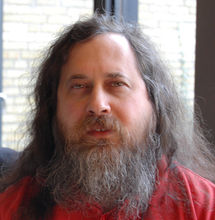
\includegraphics[height=4cm]{images/richardstallman.jpg}
  \hspace{1cm}
  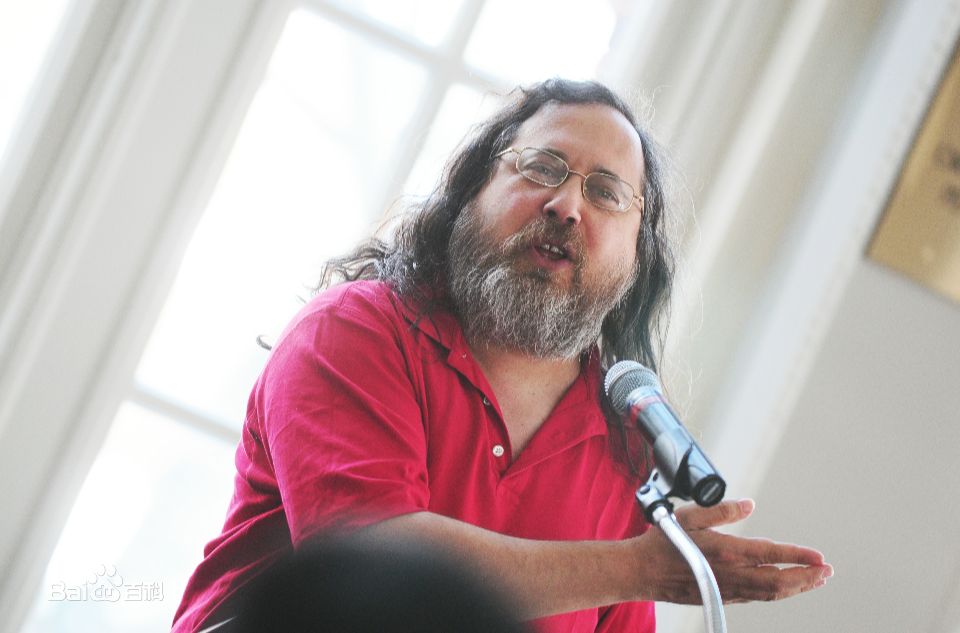
\includegraphics[height=4cm]{images/richardstallman.png}
  \label{fig:rms}
  \caption{Richard Stallman/理查德·马修·斯托曼}
\end{figure}

斯托曼对此感到气愤与无奈。在对Symbolic进行了一段时间的抗争后,他于1985年发表了著名的GNU宣言(GNU
Manifesto),正式宣布要开始进行一项宏伟的计划:创造一套完全自由免费,兼容于Unix的操作系统GNU(GNU's
Not Unix!)。之后他又建立了自由软件基金会来协助该计划。

他于1989年与一群律师起草了广为使用的GNU通用公共协议证书(GNU General
Public License, GNU
GPL),创造性地提出了\cqh 反版权\cqt (或\cqh 版权属左\cqt ,或\cqh 开权\cqt ,copyleft)的概念。
同时,GNU计划中除了最关键的Hurd操作系统内核之外,其他绝大多数软件已经完成。

1991年芬兰大学生Linus
Torvalds在GPL条例下发布他自己创作的Linux操作系统内核,至此GNU计划正式完成,操作系统被命名为GNU/Linux(或简称Linux)。

斯托曼是一名坚定的自由软件运动倡导者与其他提倡开放源代码的人不同,斯托曼并不是从软件质量的角度而是从道德的角度来看待自由软件。他认为使用专利软件是非常不道德的事,只有附带了源代码的程序才是符合其道德标准的。对此许多人表示异议,并也因此有了自由软件运动与开源软件运动之分。

\textbf{GNU}

斯托曼做了一个与Unix兼容的操作系统。这样容易被移植,而且Unix用户可以方便地转移过来。这个系统的名字就叫GNU,这个名字的确定就是遵循黑客传统,是一个递归的缩略词:\cqh GNU
IS NOT UNIX。\cqt 

但一个操作系统并不仅仅意味着一个内核(管理磁盘,内存分配等),而且仅能运行其他程序也是不够的。一个完整的操作系统,还需要有指令处理器、汇编程序、编译器、解释程序、调试器、文本编辑器、邮件软件等等,这样才能形成一个完整的系统。斯托曼决定尽可能采用已有的自由软件,比如一开始他将Tex作为主要的文本格式标识符,几年后他又用X
Window系统作为GNU的窗口系统。

1984年1月,斯托曼已启动了GNU计划,他担心MIT会要求产品的所有权,会给产品强加入他们的销售条件,最终又会成为专有软件,因而他辞去了MIT工作。辞职后,他为买不起电脑而发愁时,发现自己原来在人工智能实验室的办公室,还没有分给其他人用时,他就每天晚上溜进去工作。

GNU工程启动后,斯托曼听说有一个自由大学编译器套件(VUCK)。他去询问能否用入GNU。答复是嘲弄式的,说对大学是自由的,但对软件本身不行。于是,他决定为GNU编写的第一个软件就是一个多语言、多平台的编译器。他想利用Pastel编译器的源代码,但最终放弃。他从头编写了新的编译器,名为GCC(the
GNU Compiler Collection)。

1984年9月,斯托曼开始开发字处理器GNU
Emacs,1985年初,它开始可以工作。这使它可以在Unix系统上进行文本编辑。此时,许多人想使用Emacs,因此一个现实的问题是:如何传播它?

当然,他将其放到了MIT计算机的匿名服务器上。但那时互联网还未普及,人们很难通过FTP获得拷贝,而且失业的斯托曼也需要收入。于是,他宣布任何人都可以用150美元的价格获得全部程序。当然,所支付的费用是远低于当时的专有软件的价格的,并且用户可以得到软件的源代码。这样,自由软件的分销商业模式就此诞生。如今,整个基于Linux的GNU系统都是如此。

\hypertarget{linus-torvalds}{%
\subsection{Linus Torvalds}\label{linus-torvalds}}

本节摘自\href{https://baike.baidu.com/item/\%E6\%9E\%97\%E7\%BA\%B3\%E6\%96\%AF\%C2\%B7\%E6\%89\%98\%E7\%93\%A6\%E5\%85\%B9/2122821?fr=aladdin\&fromid=400810\&fromtitle=linus}{百度百科},有改动。

\textbf{个人经历}

林纳斯·本纳第克特·托瓦兹(Linus Benedict
Torvalds),1969年12月28日出生于芬兰赫尔辛基市。父亲尼尔斯·托瓦兹(Nils
Torvalds)是一名活跃的共产主义者及电台记者,曾当选芬兰共产党中央委员会委员。托瓦兹家族属于在芬兰占6\%的少数民族芬兰瑞典人。他毕业于赫尔辛基大学计算机系,1997年至2003年在美国加州硅谷任职于全美达公司(Transmeta
Corporation),现受聘于开放源代码开发实验(OSDL:Open Source Development
Labs,
Inc),全力开发Linux内核。与妻子托芙(Tove,芬兰前女子空手道冠军)育有三个女孩。

与很多其他黑客不同,托瓦兹行事低调,一般很少评论商业竞争对手(例如微软)产品的好坏,但坚持开放源代码信念,并对微软等对手的FUD战略大为不满。

\begin{figure}[!htp]
  \centering
  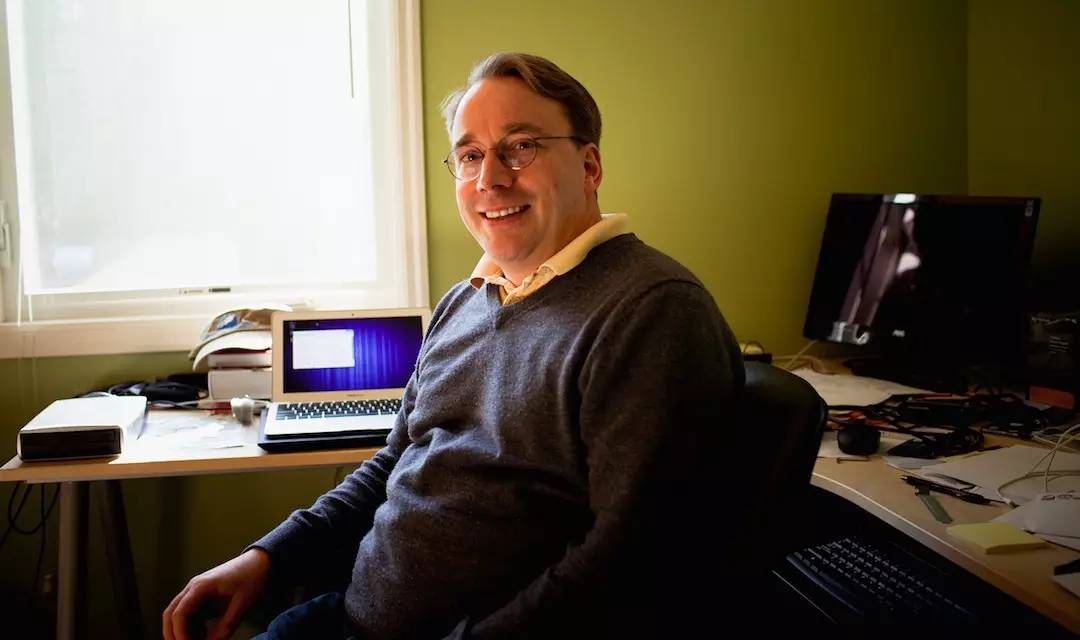
\includegraphics[height=4cm]{images/linus.jpg}
  \hspace{1cm}
  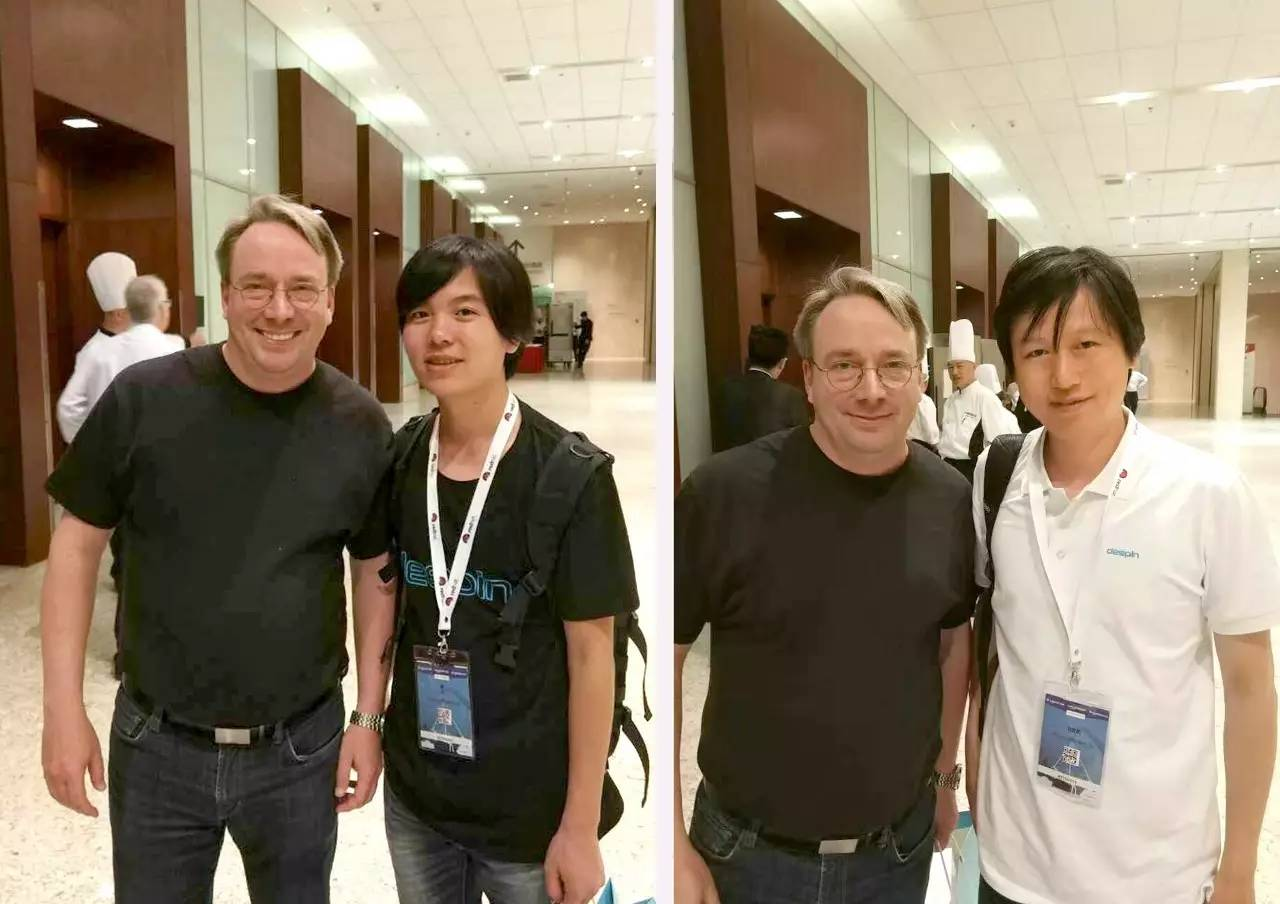
\includegraphics[height=4cm]{images/deepin-linus.jpeg}
  \label{fig:linus}
  \caption{Linus Benedict Torvalds/林纳斯·本纳第克特·托瓦兹}
\end{figure}

例如,在一封回应微软资深副总裁Craig
Mundie有关开放源代码运动的评论(Mundie批评开放源代码运动破坏了知识产权)的电子邮件中,托瓦兹写道:\cqh 我不知道Mundie是否听说过艾萨克·牛顿(Isaac
Newton)爵士?他不仅因为创立了经典物理学(以及他和苹果的故事)而出名,也还因为说过这样一句话而闻名于世:我之所以能够看得更远,是因为我站在巨人肩膀上的缘故。\cqt 托瓦兹又说道:\cqh 我宁愿听牛顿的也不愿听Mundie的。他(牛顿)虽然死了快300年了,却也没有让房间这样得臭气熏天。\cqt 

现年49岁的林纳斯目前受聘于开放源代码开发实验室(OSDL,Open Source
Development
Labs),全身心的开发Linux内核。尽管这位年轻人看上去毫不起眼,比如林纳斯曾在他的自传《乐者为王》(Just
for
Fun)中自嘲:\cqh 我是一个长相丑陋的孩子,凡是见过我小时候照片的人,都会觉得我的相貌酷似河狸。再想象一下我不修边幅的衣着,以及一个托瓦兹家族祖祖辈辈遗传下来的大鼻子,这样,在你脑海中我的模样就形成了。\cqt 但这丝毫也影响不了林纳斯对整个商业社会的巨大价值---Linux代表着网络时代新形式的开放知识产权形态,这将从根基上颠覆以Windows为代表的封闭式软件产权的传统商业模式。更重要的是,这样的颠覆早已悄悄的出现在了商业社会的各个角落。

\textbf{Linux}

颠覆世界的\cqh 自由主义教皇\cqt 林纳斯。

\cqh 有些人生来就具有统率百万人的领袖风范;另一些人则是为写出颠覆世界的软件而生。唯一一个能同时做到这两者的人,就是托瓦兹。\cqt 美国《时代》周刊对\cqh Linux之父\cqt 林纳斯·托瓦兹(Linus
Torvalds)给出了极高的评价。甚至,在《时代》周刊根据读者投票评选出的二十世纪100位最重要人物中,林纳斯居然排到了第15位,而从20世纪的最后几年就开始霸占全球首富称号的盖茨不过才是第17位。

林纳斯的出名和\cqh 重要\cqt 来得并没什么先兆,尽管这个1969年出生在芬兰赫尔辛基的天才在年少时就已经颇具黑客神韵---对于电脑的着迷使他很早就能够驱使电脑做事情,对一切细节也都能控制自如。但当林纳斯在1991年就读于赫尔辛基大学期间刚刚开始对Unix产生浓厚兴趣,尝试着在Minix(Unix的变种)上做一些开发工作的时候,他从来也没想过会构建出一个新操作系统的内核来。

Linux的诞生显得充满了偶然。林纳斯经常要用他的终端仿真器(Terminal
Emulator)去访问大学主机上的新闻组和邮件,为了方便读写和下载文件,他自己编写了磁盘驱动程序和文件系统,这些在后来成为了Linux第一个内核的雏形。当时,他年仅21岁。

在自由软件之父理查德·斯托曼(Richard
Stallman)某些精神的感召下,林纳斯很快以Linux的名字把这款类Unix的操作系统加入到了自由软件基金(FSF)的GNU计划中,并通过GPL的通用性授权,允许用户销售、拷贝并且改动程序,但你必须将同样的自由传递下去,而且必须免费公开你修改后的代码。这说明,Linux并不是被刻意创造的,它完全是日积月累的结果,是经验、创意和一小段一小段代码的集合体。

无疑,正是林纳斯的这一举措带给了Linux和他自己巨大的成功和极高的声誉。短短几年间,在Linux身边已经聚集了成千上万的狂热分子,大家不计得失的为Linux增补、修改,并随之将开源运动的自由主义精神传扬下去,人们几乎像看待神明一样对林纳斯顶礼膜拜。

然而,在1996年底,林纳斯突然离开赫尔辛基,只身奔赴美国硅谷,成为Transmeta公司的一员,直到2003年才离开。其中的原因曾经扑朔迷离,但现在看来,那只不过是林纳斯对于自身价值的一种现实性追求。虽然当时许多人都怀疑这会给发展中的Linux造成致命伤害,不过Linux在随后几年内的发展证明,这样的担心是多余的。

林纳斯说,Linux所取得的许多成功其实可以归结为他的缺点所致。\cqh 我很懒散,我喜欢授权给其他人。\cqt 就连Linux的企鹅形象标识也是林纳斯的妻子,曾获芬兰空手道冠军的托芙(Tove)想到的,因为林纳斯曾经在澳大利亚被一只企鹅咬过。\cqh 黑客们,不,程序员们,把在Linux和其它开放源代码项目上的工作,放在比睡觉、锻炼身体、娱乐和聚会更优先的地位。因为他们乐于成为一个全球协作努力活动的一部分---Linux是世界上最大的协作项目。\cqt 

\hypertarget{unix-}{%
\section{Unix 哲学}\label{unix-}}

参考:

\begin{itemize}
\tightlist
\item
  \url{http://s3.eurecom.fr/~balzarot/softdev/material/0_2_unix_philosophy.pdf}
\end{itemize}

因为 Linux 是类 Unix 操作系统,这里摘抄一些 Unix
哲学相关的内容,方便大家对 Linux 有个浅显的认识。

\hypertarget{unix-}{%
\subsection{Unix 哲学核心}\label{unix-}}

英语原文,

\begin{quote}
This is the UNIX philosophy:

\begin{itemize}
\tightlist
\item
  Write programs that do \textbf{one thing} and do \textbf{it well}.
\item
  Write programs to \textbf{work together}.
\item
  Write programs to handle \textbf{text streams}, because that is a
  universal interface.
\end{itemize}

\VA{--- Doug McIlroy}{}
\end{quote}

汉语译文,

\begin{quote}
这是UNIX哲学:

\begin{itemize}
\tightlist
\item
  程序,应当只做\textbf{一件事},且要\textbf{做好}。
\item
  程序,应当能够\textbf{协作}。
\item
  程序,应当能够处理\textbf{文本流},因为文本流是通用接口。
\end{itemize}

\VA{--- Doug McIlroy}{}
\end{quote}

我觉得这种哲学思想都快适合做其他事情了,分而治之,统筹协调,打好基础。对于打算从事
Unix 编程的,还可以继续深入学习,这里就不多介绍了。

\hypertarget{unix-}{%
\subsection{Unix 哲学下的用户}\label{unix-}}

Unix
相信用户,并赋予其极多选择极大权力,但也要求用户必须花足够多的时间来学习。

但是,\cqh 只要是个人,就会犯错误的\cqt ,这种 Unix
绝对信任也有极大的危害。网上仅仅 \passthrough{\lstinline!rm -rf ./!}
误删就害死了不少人。而且要花费非常多的时间来学习一门操作系统,也是一个极大的弊端。正是这种种缺陷,催生了各种发行版,后面\ref{chap:linux-intro:distro}节再说。

\hypertarget{unix-}{%
\subsection{Unix 哲学的对手}\label{unix-}}

以当前桌面领域普及最广的 Windows\index{Windows} 系统为对照,看看 Windows
和 Unix 的区别。

Unix 是以科学家和程序员为用户群体的,但是类 Unix 的 Linux
的用户群体也开始包含普通吃瓜群众了。而 Windows
是以所有人,当然包括那些普通群众,而且最主要的就是普通群众,为用户群体的。基于不同的目标用户,Unix
要提供各种可能性,让目标用户,\cqh 来玩坏自己,实现各种功能,尽情的发挥自己的聪明才智\cqt ,相当于给用户提供了大量积木块;Windows
则要提供傻瓜式服务,防备着你玩坏了,对你各种猜测,引导你去完成特定的任务,以免犯错,相当于给用户提供了一个个成品玩具。用参考文章的一句话来说\cqh Unix
的使用依赖用户的聪明才智,Windows
则隐藏这些技巧于操作系统和软件内部\cqt 。

下面来分析一下,这两者的优缺点。

\begin{itemize}
\tightlist
\item
  Windows
  的优点,降低用户的学习时间成本;缺点,倡导傻瓜式用户,限制用户的灵活发挥。
\item
  Unix 的优点,提供更多的可能性;缺点,增大用户的学习时间成本。
\end{itemize}

当然,随着 GNU/Linux 发行版的活跃发布,Unix
哲学的一些缺点也在被慢慢修正。也许,未来的 GNU/Linux
发行版既能提供易操作的成品玩具,也附带大量灵活的积木零件,综合两者的优势,更方便也更灵活更高效。

\hypertarget{chap:linux-intro:distro}{%
\section{GNU/Linux 发行版的出现}\label{chap:linux-intro:distro}}

如果完全从 Unix
哲学起步,用源代码一步步编译为可用软件,对广大普通用户来说就太难了,GNU/Linux
也将举步维艰。以 Linux 为内核,外加 GNU
的一些软件和服务,添上图形界面等,满足用户的基本需求,这样发行版的出现,能够很好的解决上述难题,也就流行开来了。GNU/Linux
发行版的出现,也是对 Unix 哲学的一种实践补充。所以各发行版的目标和口号和
Unix
哲学还是有一定的区别,比如深度公司的口号\cqh 免除新手痛苦、节约老手时间\cqt ,就不会说,\cqh 单一高效\cqt 。

发行版的历史就不说了,当前常见的发行版有这两大类,Red Hat 系列和 Debian
系列,当然还有 slackware 以及其他有特殊目的的发行版等等,这里略过他们。

\hypertarget{red-hat-}{%
\subsection{Red Hat 系}\label{red-hat-}}

Red Hat 系列发行版是一个非常流行的 GNU/Linux 发行版,属于 Red Hat
公司,代码开源,通过售卖服务以及培训等收费,起步非常早。采用非常好用的
rpm
软件包管理器,系统非常稳定,安装简单,有图形化操作界面。该公司对近期比较热门的领域,比如云计算等也有涉猎。旗下主要有企业稳定版的
Red Hat Enterprise Linux 和功能实验版 Fedora
两类操作系统。另外有社区企业版 centos 发行版是完全复制 Red Hat
Enterprise Linux 源码,并剔除 Red Hat
公司标志后编译成的发行版,稳定可靠,也值得了解一下。

\hypertarget{debian-}{%
\subsection{Debian 系}\label{debian-}}

\href{https://baike.baidu.com/item/Debian}{Debian} 也是一个早期的
GNU/Linux 发行版,有非常好用的软件包管理器,软件包为 deb
格式,系统稳定性非常高。有众多的发行版基于或者追根溯源到
Debian,比如本书介绍的对象 Deepin 深度操作系统,以及比较著名的
Ubuntu,国际排名非常靠前的 Linux Mint,网络安全必备的 Kali
Linux,老旧电脑挚爱的 Lubuntu 等发行版。本书介绍的很多技术均适用于
Debian 系列的发行版。

\hypertarget{-linux-}{%
\section{如何提高自己的 Linux 技术}\label{-linux-}}

参考网页:

\begin{itemize}
\tightlist
\item
  \url{https://www.tecmint.com/free-online-linux-learning-guide-for-beginners/}
\item
  \url{https://www.cnblogs.com/evilqliang/p/6247496.html}
\item
  \url{https://blog.csdn.net/erlian1992/article/details/54586156}
\end{itemize}

最好的办法就是\textbf{直接上手!}古人云\cqh 临渊羡鱼,不如退而结网\cqt 。下载一个
Linux 发行版,安装在自己的电脑上,平常多用,偶尔折腾一下,就差不多了。

\hypertarget{-gnulinux-}{%
\subsection{首先安装 GNU/Linux 操作系统}\label{-gnulinux-}}

当然这里肯定首先推荐 \href{https://www.deepin.org/}{Deepin}
深度操作系统,比较符合中国人的操作习惯。另外也可选择
\href{https://www.ubuntu.com/global}{Ubuntu}
的一些分支版本,其中\href{https://www.ubuntukylin.com/}{优麒麟}就是做得比较好的一个发行版。
如果电脑配置不够高,或者比较老旧,也可用选择轻量版的
\href{https://lubuntu.net/}{Lubuntu}。电脑配置比较高的,也可用试着在虚拟机,比如
\href{https://www.virtualbox.org/}{VirtualBox}
虚拟机内安装上述这些操作系统。

\subsection{平常多用}

GNU/Linux
的部分发行版在某些情况下,已经能够满足我们的日常工作生活需要。在平常使用不需要太折腾的前提下,我们完全可以多用、经常用。

欧阳修《卖油翁》提到\cqh 无他,惟手熟尔。\cqt  Linux
技术也是\cqh 学而时习之,不亦说乎\cqt 的事情,用多了,自然知道咋回事啦。就像\cqh 熟读唐诗三百首,不会作诗也会诌\cqt 。使用熟练后,我们就会发现
Linux 也是可以提高办公效率的好工具。

\subsection{多问多记}

很喜欢毛泽东的读书方法\cqh 不动笔墨不看书\cqt ,遇到问题及时去查资料,然后记录下来,很有助于技术水平的提高。笔者曾在某公司实习,不得已整天跟
vim
打交道,刚入门也是效率低下,后来在身边好友帮助下以及网上搜索资料,慢慢写\href{https://my.oschina.net/bubifengyun/blog/163516}{博客},也开始有点爱上
vim 了,半年下来,vim
码字母也能贼溜了。学习就是一个慢慢积累的过程,谁也不能一口吃成大胖子。曾经有一位日本人说\cqh 赵先生,中国有五千年历史呢,咱们不急,慢慢来\cqt 。慢慢来不等于不来,我们需要时刻督促自己不停的学习,\cqh 活到老学到老\cqt 。

\subsection{定个计划}

当你有一定认识后,你就会自觉不自觉的制定计划了,也会掌握更多的学习方法,这里我就不废话了。上面参考网页都是一些不错的经验介绍,希望对您有所帮助。

\section{总结}

本文首先根据用户角色,介绍了 GNU/Linux
操作系统的用途范围。通过介绍斯托曼和林纳斯两人的经历,附带讲解了 GNU 和
Linux 的发展历史,以及 GPL 协议的一些内容。接着介绍了 Unix
哲学相关的内容,最后对如何学习 GNU/Linux 提出了一些个人观点。

\hypertarget{chap:linux-desktop-intro}{%
\chapter{Linux 桌面系统简介}\label{chap:linux-desktop-intro}}

通过阅读本章,你将会了解到以下几项内容。

\begin{itemize}
\tightlist
\item
  从 Live CD/DVD 运行系统
\item
  X Window 系统
\item
  新秀 Wayland 的评价
\item
  常见的桌面环境(Desktop Environments)简介
\end{itemize}

随着技术的发展,电脑桌面操作系统也在不断的完善,虽然不能说是夕阳产业,但也在趋向一个完美的天花板。个人认为很多在
windows 和苹果桌面操作系统下的软件和操作体验,在 Linux
桌面这边一定会慢慢实现并赶上来的。未来软件会趋同,会跨平台。目前为止,
Linux 桌面系统下已经有足够多的软件满足一般的日常生活需求了。

\hypertarget{-live-cddvd-}{%
\section{运行 Live CD/DVD 试用系统}\label{-live-cddvd-}}

本文一直强调\cqh 能动手的就不要光动口\cqt ,意思就是最好安装 GNU/Linux
操作系统。如果您不喜欢安装,也可用在不安装的前提下试用该系统。下面介绍如何试用系统。当然下载安装镜像还是不可避免的。

\subsection{下载深度系统}

下载深度操作系统系统最新版本的镜像文件(以便您能够体验到最新特性),下载地址:\url{https://www.deepin.org/download/}
如图\ref{fig:livecd}所示,

\begin{figure}

\includegraphics{linux-desktop-live} \caption[如果只是试用请选择 Live 系统]{如果只是试用请选择 Live 系统}\label{fig:livecd}
\end{figure}

如果您只是想试用系统,可以选择下载\textbf{Live 系统}。

\emph{注意:为了更加专注系统的发展,deepin
15.4版本将不再提供32位官方iso镜像,如需获取和技术支持,请发送邮件到
\href{mailto:support@deepin.org}{\nolinkurl{support@deepin.org}}。}

\hypertarget{u}{%
\subsection{把系统写到U盘里}\label{u}}

安装说明: \url{https://www.deepin.org/installation/}

现在流行 U 盘安装,当然也可用光盘安装。下面只介绍 U
盘启动器的制作,到\href{https://www.deepin.org/original/deepin-boot-maker/}{这里}下载系统启动盘制作工具。
根据自己操作系统情况请选择对应版本。另外也可用选择其他的制作软件,比如
Ultraiso
软件,网上搜索\cqh 使用UltraISO(软碟通)制作U盘启动盘完整教程\cqt ,可以找到相当多的资料,这里从略。

\subsection{开始试用}

试用版有一些功能受限,但是可以感受一下。不过还是强烈建议安装正常版本的软件。

参考:

\begin{itemize}
\tightlist
\item
  \url{https://bbs.deepin.org/forum.php?mod=viewthread\&tid=157091}
\item
  \url{http://wiki.deepin.org/wiki/\%E4\%BD\%93\%E9\%AA\%8C\%E5\%AE\%89\%E8\%A3\%85}
\end{itemize}

\hypertarget{x-window-}{%
\section{X Window 系统简介}\label{x-window-}}

当前主要的linux桌面发行版基本都是采用X Window 系统来提供桌面服务。

X
Window是一种以位图方式显示的软件窗口系统,最初是1984年麻省理工学院的研究成果,之后变成UNIX、类UNIX、以及OpenVMS等操作系统所一致适用的标准化软件工具包及显示架构的运作协议。

X
Window通过软件工具及架构协议来建立操作系统所用的图形用户界面,此后则逐渐扩展适用到各形各色的其他操作系统上,几乎所有的操作系统都能支持与使用X
Window,GNOME和KDE也都是以X Window为基础建构成的。

X
Window向用户提供基本的窗口功能支持,而显示窗口的内容、模式等可由用户自行定制,在用户定制与管理X
Window系统时,需要使用窗口管理程序,窗口管理程序包括AfterStep、Enlightenment、Fvwm、MWM和TWM
Window Maker等,供习惯不同的用户选用。
可以定制的窗口环境在给用户带来了个性化与灵活性的同时,要求用户有相对比较高的使用水平,不过这种机制带来的好处也是明显的,它不象Microsoft
Window那样将窗口元件的风格、桌面、操作方式等千篇一律地规定死,只可以换一下墙纸、图标、调整字体大小等等,在X
Window系统中可以有多种桌面环境的选择。

\subsection{基本部件}

X系统由三个相关的部分组成:服务端(Server)、客户端(Client)和通讯通道 (communication
channel)。

\textbf{服务端(Server)}

Server是控制显示器和输入设备(键盘和鼠标)的软件。Server可以创建视窗,在视窗中绘图和文字,回应Client程序的\cqh 需求\cqt (requests),但它不会自己完成,只有在Client程序提出需求后才完成动作。

每一套显示设备只对应惟一的Server,而Server一般由系统供应商提供,通常无法被用户修改。对操作系统而言,Server只是一个普通的用户程序而已,因此很容易更换新版本,甚至更换成第三方提供的原始程序。

\textbf{客户端(Client)}

Client是使用系统视窗功能的一些应用程序。在X下的应用程序称做Client,原因是它是Server的客户,要求Server回应它的请求完成特定动作。

Client无法直接影响视窗行为或显示效果,它们只能送一个请求(request)给Server,由Server来完成这些的请求。典型的请求通常是\cqh 在某个视窗中写`Hello
World'的字符串\cqt ,或者从A到B划一条直线。

Client的功能大致可分为两部分:向Server发出\cqh 需求\cqt 只是它的一部分功能,其他的功能是为用户执行程序而准备的。例如输入文字信息、作图、计算等等。通常,Client程序的这一部分是和X独立的,它对于X几乎不需要知道什么。通常,应用程序(特别是只大型的标准绘图软件、统计软件等)对许多输出设备具有输出的能力,而在X视窗中的显示只是Client程序许多输出中的一种,所以,Client程序中和X相关的部分只占整个程序中很小的一部分。

用户可以通过不同的途径使用Client程序:通过系统提供的程序使用;通过第三方的软件使用;或者用户为了某种特殊应用而自己编写的Client程序来使用。

\textbf{通讯通道 (Communication channel)}

Client藉著它送 ``需求'' 给Server,而Server藉著它回送状态 (status)
及一些其它的资讯 (information)。

只要 Client 和 Server
都知道如何使用通道,通道的本身并不是很重要,在系统或网路上支援通讯型态的需求是内建於系统基本的X视窗函数馆(library),所有和通讯型态有关的事都从函数馆独立出来,Client和Server之间的通讯只要藉著使用这函数馆(在标准X版为xlib)。

\textbf{Server和Client之间的通信}

Server和Client通信的方式大致有两类,对应于X系统的两种基本操作模式。

第一类,Server和Client在同一台机器上执行,它们可以共同使用机器上任何可用的通信方式做互动式信息处理。在这种模式下,X可以同其他传统的视窗系统一样高效工作。

第二类,Client在一台机器上运行,而显示器和Server则在另一台机器上运行。因此两者的信息交换就必须通过彼此都遵守的网络协议进行,最常用的协议为TCP/IP。这种通信方式一般被称为网络透明性,这也几乎是X独一无二的特性。

\subsection{用户接口}

X的设计目标之一就是能创建许多不同形式的用户接口。其他的是视窗系统提供具体的交互方式,而X只提供一般的架构,让系统创建者建造所需的交互风格。这种特性使得开发者可以在X的基础上建造全新的接口,并且可以在任何时刻根据自己的需要选用适当的接口。

一般来说,用户接口可以分为两部分。管理接口也就是视窗管理器,是命令的最高层,它负责在屏幕上创建或重建视窗,改变视窗的大小、位置,或者将视窗改变成图示等。

应用接口确定了用户和应用程序之间的交互风格,即用户如何利用视窗系统的设备程序来控制应用程序并传递输入行为。例如,如何用鼠标来选定一个选项。

\subsection{用户界面}

X刻意不去规范应用程序在用户界面上的具体细节设计,这些包括按钮、菜单和窗口的标题栏等等,这些都由窗口管理器(window
manager)、GUI构件工具包、桌面环境(desktop
environment)或者应用程序指定的GUI(如POS)等等的用户软件来提供,然而因为架构设计上保留了高度的弹性发挥空间,致使多年来X在\cqh 基础、典型、一般性\cqt 的用户界面上,也都有数目惊人的多样性选择。

在X的系统架构中,窗口管理器用于控制窗口程序的位置和外观,其界面类似Microsoft的Windows或者Macintosh(例如:KDE的KWin或者GNOME的Metacity),不过在控制机制上却截然不同(如:X提供的基本窗口管理器twm)。窗口管理器可能只是个框架(如:twm),但也可能提供了全套的桌面环境功能(如:Enlightenment)。

虽然不同的X用户界面可以有很大的差异,然而绝大多数的用户在使用X时,多是用已经打包的桌面环境,这种桌面环境不仅包含窗口管理器,还具备各种应用程序以及风格一致的界面,目前最流行的桌面环境是GNOME和KDE,二者已普遍应用于Linux操作系统上,而UNIX所用的标准桌面环境多是通用桌面环境CDE,然而有些UNIX也开始采用GNOME。

此外,X桌面环境及组件虽然很多,但同时也需要保持兼容性与互通性,这些由freedesktop
org积极与努力地维持各种不同X桌面环境的兼容性,使竞争态势下仍不失X的兼容本色。

\subsection{优缺点}

\textbf{优点}

(1)任务分工明确

客户端可以在远程电脑上执行计算任务,而X
Server仅负责复杂的图形显示,充分发挥X Server在显示上的优势。

只有X
Server服务端与硬件打交道,所有的客户端都与硬件无关,这让不同的平台上的移植变得很容易。
客户端可以在不同的电脑上运行,从巨型机到个人电脑,从而充分发挥网络计算的优越性。

X系统只负责显示图形,并不限制显示和操作的风格,因此不同的X
Window的风格并不相同,用户可以根据自己的喜好进行选择。 由于X
Window系统只提供了最基本的系统调用,而具体的视窗都有很多共性,因此要开发X应用程序,应该首先使用开发工具包,而没有必要直接使用最基本的X
Window 的系统调用,以简化编写程序的工作量。

(2)独立于操作系统

X不是内置于操作系统,它只是比用户层次稍高一些。在系统中也是一个相对独立的元件。这样做有如下优点:

\begin{itemize}
\tightlist
\item
  易于安装和改版,甚至去除。这种工作不需要重启系统,也不会对其他应用程序造成干扰。
\item
  第三方很容易支持并加强它的功能。
\item
  X不会制定操作系统,只是一个标准,这也是第三方开发软件的原动力。
\item
  为了开发者。在Server上进行工作时,如果程序异常中断,只会影响到视窗系统,不会造成机器的损坏或操作系统内核的破坏。
\end{itemize}

\textbf{缺点}

(1)稳定性不强

在PC世界里,需要第三方硬件驱动的非主流的个人计算机软件往往不能支持那些专为Microsoft
Windows出品的设备。X
Window也不例外,它的实现往往缺少较新(或者非常旧)的高效的显卡驱动。 X
Window的C/S体系(C/S架构)设计在应用程序和显示硬件之间多加了一层软件,导致绘图效率下降,所以引起了一些批评。
X也被批评提供了过多的对硬件的直接访问,从而影响了系统的稳定性。

(2)不规范的用户界面

X刻意不去规范用户界面和程序之间大多数的通信,导致出现了许多非常不同的界面,同时造成程序之间协同的困难;而客户机之间的互操作规范ICCCM以难以正确实现而闻名。后来的标准化尝试,也于事无补。长久以来这已经成为用户和程序员的噩梦。
直到最近,X也没有好地解决显示与打印机所打印的内容一致性(所见即所得)的解决方案。

(3)网络通信能力弱

X不能像VNC那样把客户端的通信从一个服务端卸下然后再附加到另一个上,但现在正在为X增加此功能的工作,另外还要实现通过VNC实现X
Server的显示。 X
Server和远端客户机之间的网络通信使用明文的缺陷,让攻击者使用封包截取程序就能够截获和阅读它。这一缺陷一般可以通过在SSH通信上使用X来解决。
设备中立和客户端与服务端的分离还带来了一定性能开销。

参考:

\begin{itemize}
\tightlist
\item
  \url{https://baike.baidu.com/item/X\%20Window/7249336?fr=aladdin}
\end{itemize}

\hypertarget{-wayland}{%
\section{王勇谈 Wayland}\label{-wayland}}

本篇大部分为转载,有改动。

Wayland是一个简单的\cqh 显示服务器\cqt (Display Server),与X
Window属于同一级的事物,而不是仅仅作为X Window下X Server的替代(注:X
Window下分X Server和X Client)。也就是说,Wayland不仅仅是要完全取代X
Window,而且它将颠覆Linux桌面上X Client/X
Server的概念,以后将没有所谓的\cqh X Client\cqt 了,而是\cqh Wayland
Client\cqt 。更确切的说,Wayland只是一个协议(Protocol),就像X
Window当前的协议------X11一样,它只定义了如何与内核通讯、如何与Client通讯,具体的策略,依然是交给开发者自己。所以Wayland依然是贯彻\cqh 提供机制,而非策略\cqt 的Unix程序。

Wayland相对于古老的X11来说最大的提升是,Gtk/Qt
这些图形库进行图形绘制时,不用像X11那样发送绘制消息到XServer来进行绘制,而是由Client自己进行图形绘制,Wayland只用担任图层混合器的作用。这样不但减少了X
Client和X
Server之间不必要的通讯,而且因为由Client自己进行渲染,所以很多画面撕裂和闪屏的现象从原理上就避免了。

大家可以看一下下面的两张架构图,图\ref{fig:xw-x}和图\ref{fig:xw-w},来理解两者的差别:

\begin{figure}
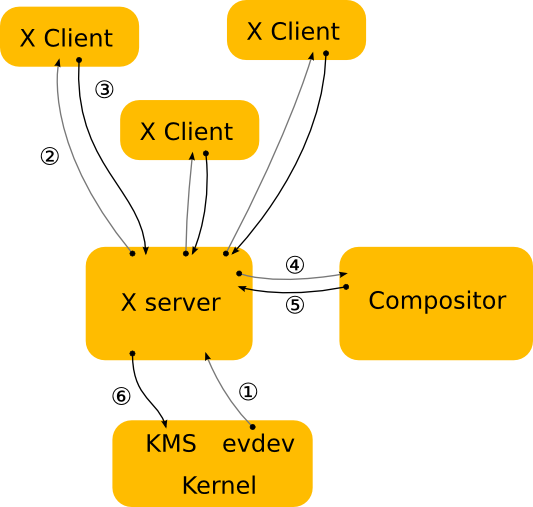
\includegraphics{X-architecture} \caption[X 架构图]{X 架构图}\label{fig:xw-x}
\end{figure}

\begin{figure}
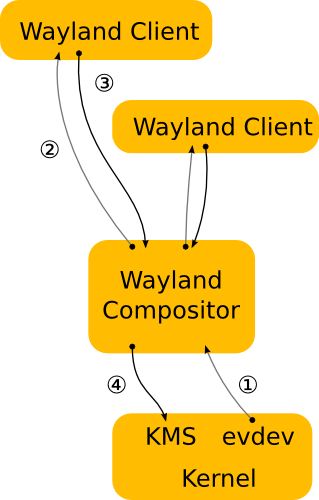
\includegraphics{Wayland-architecture} \caption[Wayland 架构图]{Wayland 架构图}\label{fig:xw-w}
\end{figure}

Wayland
因为要彻底从技术架构上颠覆Linux几十年X11的渲染方式,不论从架构设计还是代码实现上都会非常复杂,不但要开发协议本身,还需要开发适合Wayland的混合器和窗口管理器,最后导致Wayland
1.0稳定版一再跳票。

而Ubuntu在独立开发Unity桌面环境的同时,也仿造了Wayland的架构开发了自己的Mir显示服务器,除了等不及Wayland稳定之外,更重要的是Ubuntu要为了它的下一步宏伟计划 ``Ubuntu
Touch''
,按照Mark的设想,Mir不仅仅要像Wayland那样从原理上提升Linux图形渲染效率,而且Mir还得担负起手机和电脑融合的使命,可以让Ubuntu
Touch的手机在插上显示器底座时,手机的应用通过Mir的支持,可以直接在外接显示器上显示手机应用窗口,最终达到\cqh 当你手机放到底座时就是电脑,拿走就是手机\cqt 的设想。

不论Wayland还是Mir,虽然底层架构都非常先进,但是为了兼容现有的X11程序,它们分别开发了
XWayland 和 XMir 用于在新的显示服务器协议上支持现有的大多数 X11
程序(主要是Gtk2/Qt3/Qt4开发的大多数应用)。

具有讽刺意味的是,Wayland和Mir本来就是要解决 X11
那种不适合现代PC场景繁琐的通讯协议,甚至很多开发者为了技术的洁癖都在大力安利
Wayland/Mir ,但是最后 XWayland 和 XMir 本身的兼容实现却比 X11
的实现更加\cqh 恶心\cqt 和繁琐,包括Mir的开发者最后都放弃 XMir 的开发。

正是因为Wayland/Mir这样的技术无法彻底解决和大部分原本就基于X11协议而开发的应用的兼容性问题,最后导致基于Wayland/Mir开发的桌面系统从 \cqt 解决渲染性能问题\cqh  转变到 \cqh 无法运行很多现有Linux应用\cqt  这一个更加让用户难以接受的结果。这也是后面基于Mir开发的新版Unity难产的重要原因。

参考:

\begin{itemize}
\tightlist
\item
  \url{https://www.jianshu.com/u/E6EbkP}
\item
  \url{https://www.jianshu.com/p/86dd6e34ce91}
\item
  \url{https://baike.baidu.com/item/Wayland/7429696?fr=aladdin}
\end{itemize}

\section{常见的桌面环境}

桌面环境是为了方便用户操作电脑的一系列工具的集合。常常包括以下几个或者全部的组件。

\begin{itemize}
\tightlist
\item
  窗口管理器(Window manager)
\item
  面板(Panels)
\item
  菜单(Menus)
\item
  小工具(Widgets)
\item
  文件管理器(File Manager)
\item
  浏览器(Browser)
\item
  办公套件(Office Suite)
\item
  文本编辑器(Text Editor)
\item
  终端(Terminal)
\item
  显示管理器(Display Manager)
\end{itemize}

Linux 桌面环境有很多种,比如
Cinnamon,Unity,GNOME,KDE,XFCE,LXDE,MATE,Enlightenment,Pantheon
,以及后面详细介绍的深度桌面 DDE(Deepin Desktop Environment)等。

\hypertarget{cinnamon}{%
\subsection{Cinnamon}\label{cinnamon}}

\begin{figure}

\includegraphics{de-Cinnamon} \caption[Cinnamon 桌面环境样图]{Cinnamon 桌面环境样图}\label{fig:de-Cinnamon}
\end{figure}

图\ref{fig:de-Cinnamon},Cinnamon 桌面环境很现代很时尚,界面类似 Win
7,是 Linux Mate 的默认桌面环境,托 Linux Mate的福,也非常流行。

此桌面环境,底部有一个面板,在右下角有一个带有快速启动图标和系统托盘的时尚菜单,有一系列的键盘快捷方式方便操作,视觉效果也很棒。同时也有很好的定制功能,比如更改壁纸,添加和位置面板,添加小程序到面板,也可以添加桌面提供新闻,天气和其他关键信息等。

\begin{itemize}
\tightlist
\item
  内存使用情况:\(\approx\) 175MB
\item
  优点:

  \begin{itemize}
  \tightlist
  \item
    仿Windows的操作习惯。
  \item
    好看、特效多、小部件多
  \item
    键盘快捷键功能强大
  \item
    可定制
  \end{itemize}
\item
  缺点:

  \begin{itemize}
  \tightlist
  \item
    与其他桌面相比太耗内存
  \item
    可定制的功能还不够强大
  \end{itemize}
\end{itemize}

\hypertarget{gnome}{%
\subsection{GNOME}\label{gnome}}

\begin{figure}
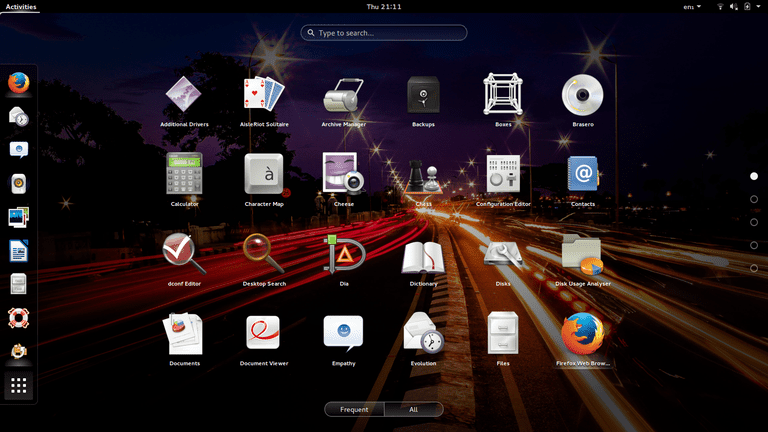
\includegraphics{de-GNOME} \caption[GNOME 桌面环境样图]{GNOME 桌面环境样图}\label{fig:de-GNOME}
\end{figure}

图\ref{fig:de-GNOME},GNOME桌面环境,包括 GNOME2 和
GNOME3,GNU计划的一部分,开放源码运动的一个重要组成部分,是一种让使用者容易操作和设定电脑环境的工具,目标是基于自由软件,为Unix或者类Unix操作系统构造一个功能完善、操作简单以及界面友好的桌面环境,是GNU计划的正式桌面环境。

\begin{itemize}
\tightlist
\item
  内存使用情况:\(\approx\) 250MB
\item
  优点:

  \begin{itemize}
  \tightlist
  \item
    现代的
  \item
    有大量的核心应用程序和开发工具包,使得开发人员易于创建丰富的应用程序。
  \item
    功能强大的键盘快捷键
  \item
    搜索过滤功能强悍
  \end{itemize}
\item
  缺点:

  \begin{itemize}
  \tightlist
  \item
    太耗内存
  \item
    可定制性极差
  \end{itemize}
\end{itemize}

\hypertarget{kde}{%
\subsection{KDE}\label{kde}}

\begin{figure}

\includegraphics{de-KDE} \caption[KDE桌面环境样图]{KDE桌面环境样图}\label{fig:de-KDE}
\end{figure}

图\ref{fig:de-KDE},KDE桌面环境类似 Cinnamon,仿 Win
7。底部有一个面板,菜单,快速启动栏和系统托盘图标。可以在桌面上添加新闻和天气等小部件。默认安装有大量的应用程序。

\begin{itemize}
\tightlist
\item
  内存使用情况:\(\approx\) 300MB
\item
  优点:

  \begin{itemize}
  \tightlist
  \item
    仿Windows的操作习惯
  \item
    提供大量的默认应用程序,包括Web浏览器和邮件客户端。
  \item
    很多小部件
  \item
    可定制能力强
  \end{itemize}
\item
  缺点:

  \begin{itemize}
  \tightlist
  \item
    太耗内存
  \end{itemize}
\end{itemize}

\hypertarget{lxde}{%
\subsection{LXDE}\label{lxde}}

\begin{figure}

\includegraphics{de-LXDE} \caption[LXDE 桌面环境样图]{LXDE 桌面环境样图}\label{fig:de-LXDE}
\end{figure}

图\ref{fig:de-LXDE},LXDE桌面环境非常适合旧计算机。能提供一些非常基础的功能。

\begin{itemize}
\tightlist
\item
  内存使用情况:\(\approx\) 85MB
\item
  优点:

  \begin{itemize}
  \tightlist
  \item
    非常小巧,适合旧电脑和配置较差的计算机
  \item
    强大的定制能力
  \end{itemize}
\item
  缺点:

  \begin{itemize}
  \tightlist
  \item
    默认应用程序较少
  \item
    可用应用程序相比其他桌面环境体验感觉不够好
  \end{itemize}
\end{itemize}

参考:

\begin{itemize}
\tightlist
\item
  \url{https://wiki.deepin.org/wiki/Linux\%E6\%A1\%8C\%E9\%9D\%A2\%E6\%BC\%94\%E8\%BF\%9B}
\item
  \url{https://www.deepin.org/developer-community/architectural-design/}
\item
  \url{https://itsfoss.com/best-linux-desktop-environments/}
\item
  \url{https://www.lifewire.com/best-linux-desktop-environments-4120912}
\item
  \url{https://www.tecmint.com/best-linux-desktop-environments/}
\end{itemize}

\hypertarget{-1}{%
\section{总结}\label{-1}}

本章介绍了如何在不安装系统的情况下,试用 GNU/Linux 系统。然后介绍了 X
Window 系统的概况,同时附带介绍了当前新技术 Wayland
的状况。最后列举了常见的几种桌面环境。

\hypertarget{chap:deepin-intro}{%
\chapter{\texorpdfstring{深度操作系统\index{深度操作系统}简介}{深度操作系统简介}}\label{chap:deepin-intro}}

\emph{本章打算重构,安装操作系统后移,把系统结构转移到这里来。}
通过阅读本章,你将会了解到以下几项内容。

\begin{itemize}
\tightlist
\item
  武汉深之度科技有限公司简介
\item
  深度操作系统的安装
\item
  深度桌面使用
\item
  深度桌面常用软件
\end{itemize}

摘自:\href{https://www.deepin.com/}{深度商业官网}、\href{https://www.deepin.org/}{深度社区官网}及\href{http://wiki.deepin.org/wiki/DEEPIN_\%E6\%A1\%8C\%E9\%9D\%A2\%E7\%B3\%BB\%E7\%BB\%9F\%E5\%AE\%89\%E8\%A3\%85\%E6\%A6\%82\%E8\%BF\%B0}{深度百科}。已获\href{https://bbs.deepin.org/forum.php?mod=viewthread\&tid=39632\&page=10\#pid377474}{许可}。

\section{\texorpdfstring{深度科技简介\index{深度科技}}{深度科技简介}}

\textbf{武汉深之度科技有限公司}

武汉深之度科技有限公司(以下简称深度科技)成立于 2011 年,是专注基于
Linux 的国产操作系统研发与服务的商业公司。

作为国内顶尖的操作系统研发团队,深度科技以提供安全可靠、美观易用的国产操作系统与开源解决方案为目标,拥有操作系统研发、行业定制、国际化、迁移和适配、交互设计、支持服务与培训等多方面专业人才,能够满足不同用户和应用场景对操作系统产品的广泛需求。

\begin{figure}

\includegraphics{about-us_content_logo} \caption[武汉深之度科技有限公司标志]{武汉深之度科技有限公司标志}\label{fig:deepin-inc}
\end{figure}

深度科技作为国产操作系统生态的打造者,不但与各芯片、整机、中间件、数据库等厂商结成了紧密合作关系,还与
360、金山、网易、搜狗等企业联合开发了多款符合中国用户需求的应用软件。深度科技的操作系统产品,已通过了公安部安全操作系统认证、工信部国产操作系统适配认证、入围国管局中央集中采购名录,并在国内党政军、金融、运营商、教育等客户中得到了广泛应用。

截止到 2015 年,深度操作系统下载超过 4000 万次,提供 30
种不同的语言版本,以及遍布六大洲的 70
多个镜像站点的升级服务。在全球开源操作系统排行榜上,深度操作系统长期保持前
20 名,也是排名最高的中国操作系统产品。

未来,深度科技将继续秉承开源和创新精神,以操作系统的自主可控替代为契机,争取在三年内成为中国市场主要操作系统供应商,五年后成为具备国际影响力的主流操作系统厂商。

\textbf{深度操作系统项目}

深度操作系统 是一个致力于为全球用户提供美观易用、安全可靠体验的 Linux
发行版。它不仅仅对最优秀的开源产品进行集成和配置,还基于 Qt
技术开发了深度桌面环境和深度控制中心,并且开发了一系列面向日常使用的深度特色应用如深度商店、深度截图、深度音乐、深度影院等。深度操作系统非常注重易用的体验和美观的设计,对于大多数用户来说,它易于安装和使用,能够很好的代替
Windows 系统进行工作与娱乐。

\begin{figure}
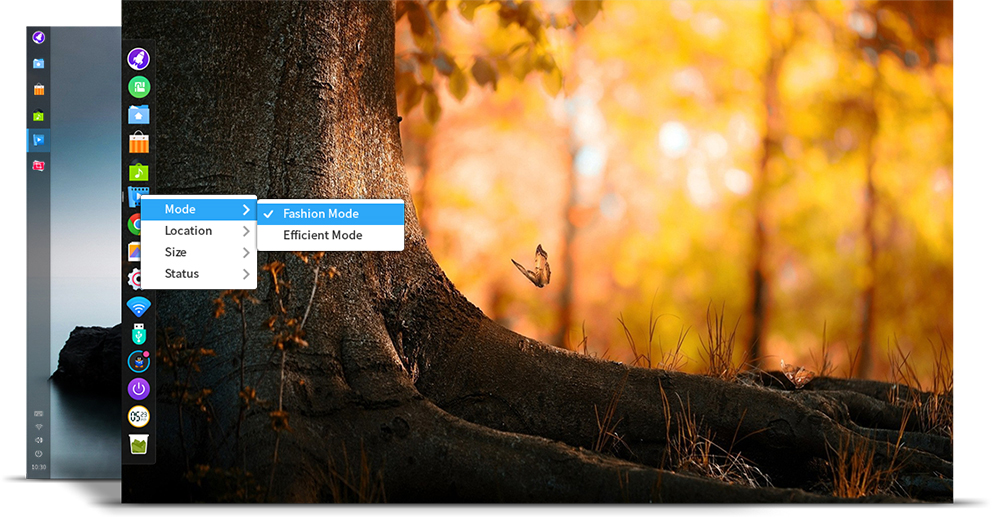
\includegraphics{en_about-us_content_sys} \caption[深度操作系统桌面]{深度操作系统桌面}\label{fig:deepin-os}
\end{figure}

深度操作系统的历史可以追溯到 2004 年,其前身 Hiweed Linux
是中国第一个基于Debian的本地化版本。在 2008 年更名为深度操作系统,2011
年获得商业投资,已经建立起国内少有的拥有员工数十人专注于桌面 Linux
发行版的团队。深度操作系统与Sogou, WPS, Maxthon
等合作伙伴进行了多方位合作,共同打造基于 Linux
系统的生态系统。同时,我们还在努力解决迁移 Windows
平台软件带来的各种兼容性问题,以便用户平滑的过渡到开放安全的 Linux
平台上来。

对个人用户来说,使用深度操作系统不但完全免除了购买费用,而且不会被流行的各种病毒和木马感染。对于政府和企业用户,由于源代码开放可控,绝无后门隐患,安全性也更有保障,大大降低了维护代价和购买防护软件的费用。

近年来,深度操作系统发展迅速,获得全球40多个国家用户的支持,累计下载量数千万次,并成为在Distrowatch
上排名最高的中国 Linux 操作系统发行版。

非常欢迎您尝试深度操作系统作为您工作和生活的伙伴,作为中国鲜少地专注于桌面操作系统的团队,我们相信它将给您带来完全不同的体验!

注:深度论坛网友
\href{https://bbs.deepin.org/forum.php?mod=viewthread\&tid=145309\&page=1\#pid378170}{licardo}
建议,\cqh\textbf{国产操作系统}\cqt 改为\cqh\textbf{国内发行版}\cqt 。深以为然。但是考虑到转帖的别人的文章,就保留不变了,特此说明。

\section{深度操作系统的安装}

\subsection{安装方案}

\textbf{全新安装 DEEPIN 单系统}

所谓安装 deepin
单系统,即计算机上不保留其他操作系统,并且使用单独的分区格式化后安装
deepin。

准备工作:

\begin{itemize}
\tightlist
\item
  如果是全新的电脑,或者硬盘中的文件数据均已备份无需保留,则直接使用光盘或优盘启动电脑进入安装操作即可。
\item
  如果电脑中已有文件数据,则可以在现有系统(如
  Windows)下将文件移动或备份,留出至少一个20G的空白分区;或者使用磁盘工具(推荐分区助手,下载地址)并选择一个剩余空间合适的分区进行大小调整,使磁盘中有20G以上的未分配空间或空白分区。
\end{itemize}

\textbf{与 WINDOWS 共存安装双/多系统}

在计算机上已经安装后 Windows 操作系统的情况下,如果想要保留已有 Windows
系统,则可安装双/多系统,实现 deepin 与 Windows 的共存。

与全新安装一样的,保证磁盘上有20G以上的未分配空间或空白分区即可。

\subsection{安装环境}

请确保您的电脑满足以下的配置要求,如果您的电脑配置低于以下的要求,将无法完美的体验深度操作系统:

\begin{itemize}
\tightlist
\item
  处理器:Intel Pentium IV 2GHz 或更快的处理器
\item
  内存:至少 2G 内存(RAM),4G 以上是达到更好性能的推荐值
\item
  硬盘:至少 10 GB 的空闲空间
\end{itemize}

同时,您还需要一张光盘以及光驱,如果您的电脑无光驱设备,可登录深度科技官方网站下载镜像文件并制作优盘启动盘。

\subsection{启动优盘的制作}

请使用深度科技团队开发的\href{https://www.deepin.org/original/deepin-boot-maker/}{深度启动盘软件制作工具}制作启动优盘,你也可使用压缩软件打开\href{https://www.deepin.org/download/}{深度操作系统镜像}提取。

请根据自己\textbf{操作系统类型}的不同,选择\textbf{对应操作系统的启动盘制作工具}。将优盘插入电脑后,运行深度启动盘制作工具,选择深度操作系统镜像开始制作启动盘,制作期间请不要移除优盘,制作完成请选择重启电脑。

注意:

\begin{itemize}
\tightlist
\item
  制作前请提前转移优盘中重要数据,制作时可能会清除优盘所有数据;
\item
  制作前建议讲优盘格式化为FAT32格式,以提高识别率;
\item
  部分优盘实则为移动硬盘,因此无法识别,请更换为正规优盘;
\item
  优盘容量大小不得小于8G,否则无法成功制作启动盘;
\item
  制作过程中请不要触碰优盘,以免因为写入不全导致制作失败。
\end{itemize}

\subsection{安装过程}

一般情况下电脑默认是从硬盘启动,因此,在使用光盘(优盘)安装系统之前,您需要先进入电脑的BIOS界面将光盘(优盘)设置为第一启动项。

台式机一般为 Delete 键、笔记本一般为 F2 或 F10 或 F12 键,即可进入 BIOS
设置界面。

您只需在享受一杯咖啡的时间,便可完成系统的安装。

1、将深度操作系统光盘(优盘)插入电脑光驱(USB接口)中。

2、启动电脑,将光盘(优盘)设置为第一启动项。

3、进入安装界面,选择需要安装的语言。

\leftline{\begin{minipage}{\linewidth}
\begin{center}

\includegraphics{deepin-installer1.png}
\captionof{figure}{安装界面}
\label{deepin-installer1}
\end{center}
\end{minipage}}

4、进入账户界面,输入系统用户名和密码。

\leftline{\begin{minipage}{\linewidth}
\centering

\includegraphics{deepin-installer2.png}
\captionof{figure}{账户界面}
\label{deepin-installer2}
\end{minipage}}

5、点击\textbf{下一步}。

6、选择文件格式、挂载点、分配空间等。

\leftline{\begin{minipage}{\linewidth}
\begin{center}
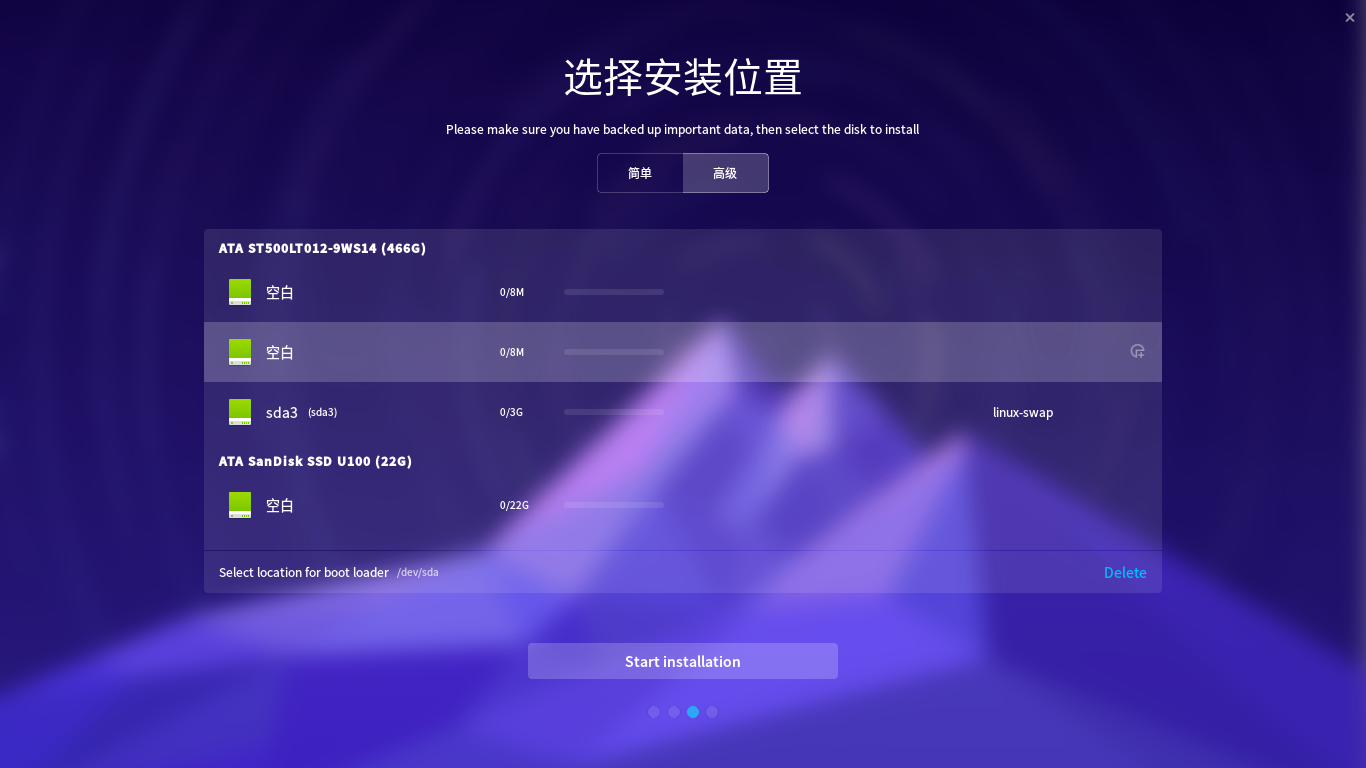
\includegraphics{deepin-installer3.png}
\captionof{figure}{磁盘挂载界面}
\label{deepin-installer3}
\end{center}
\end{minipage}}

\begin{longtable}{|L{1in}|L{1.2in}|L{1.2in}|L{1.9in}|}
\caption{\label{tab:mount}文件挂载说明} \\ \hline
\centerline{\textbf{挂载点}} & \centerline{\textbf{挂载点中文名}} & \centerline{\textbf{文件系统}} & \centerline{\textbf{大小}} \\
\hline
\rowcolor{LightCyan}
/       &   根分区(必选)     &    EXT4(推荐)     &   最少10G \\
/home   &    家目录(推荐) &   EXT4(推荐)     &     最少10G \\
\rowcolor{LightCyan}
swap    &    交换分区(可选)&    不设置         &     4G内存以下分配2G,\newline 4G以上可不分配 \\
\hline
\end{longtable}

7、点击\textbf{安装}。

8、在弹出的确认安装窗口中,点击\textbf{确定}。

9、将开始自动安装深度操作系统。

安装视频见:\url{https://www.bilibili.com/video/av16993752/}

想对安装过程有更多理解,可以阅读附录\ref{install-further-read},或者网上搜索相关教程。

\section{桌面使用}

其实深度系统自带一套学习指南\textbf{深度帮助手册}。可以按下\textbf{Super}键,也即一般电脑上微软标志的那个键,或者苹果电脑上的花键。在搜索里输入\cqh 深度帮助手册\cqt 就能够找到。打开后,可以自学很多知识,本书摘录其中部分内容。

还有另外一套帮助工具,\textbf{欢迎},同上,打开后,可以直接设置相关的选项。

\subsection{开机}

如果你使用过 Windows
操作系统,那么使用深度桌面操作系统也不是难事。这里主要讲社区版深度桌面操作系统。
开机登录后,点击\textbf{Super}键会弹出如下界面。

\leftline{\begin{minipage}{\linewidth}
\begin{center}
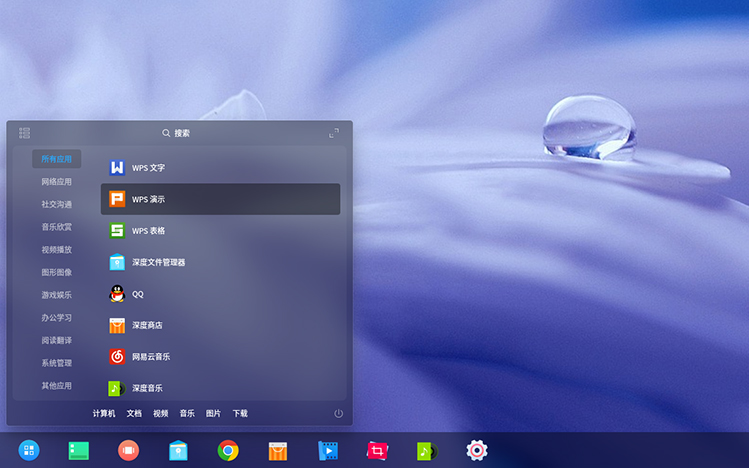
\includegraphics{deepin-desktop-1.jpg}
\captionof{figure}{启动项}
\label{deepin-desktop-1}
\end{center}
\end{minipage}}

你可以对所需要的软件进行搜索。直接点击软件图标,就可以打开软件了。分类放置的软件。在任务栏驻留的软件打开时,还会有动画显示。

\leftline{\begin{minipage}{\linewidth}
\begin{center}
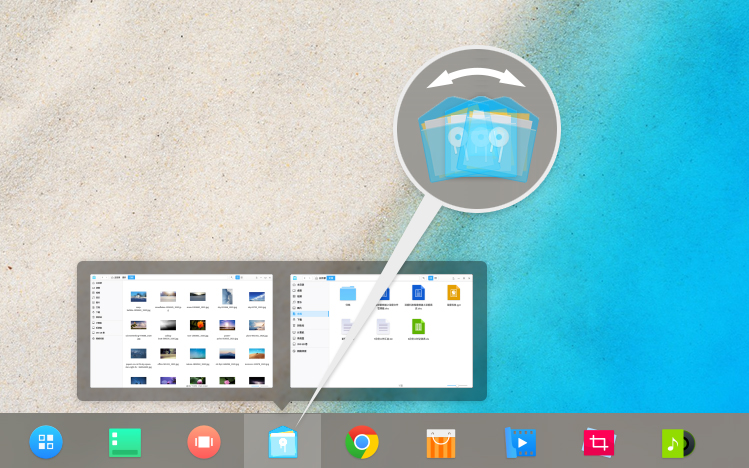
\includegraphics{deepin-desktop-2.jpg}
\captionof{figure}{任务栏打开软件动画}
\label{deepin-desktop-2}
\end{center}
\end{minipage}}

\subsection{关机}

同时按 Ctrl + Alt +
Delete,或者点击右下角关机按钮,就会弹出关机界面,如下图所示。

\leftline{\begin{minipage}{\linewidth}
\begin{center}

\includegraphics{shutdown.png}
\captionof{figure}{关机}
\label{shutdown}
\end{center}
\end{minipage}}

\hypertarget{-}{%
\subsection{控制中心-系统设置}\label{-}}

点击任务栏,或者鼠标滑向桌面右下角几次,会在右侧出现控制中心面板。如下图所示。

\leftline{\begin{minipage}{\linewidth}
\begin{center}
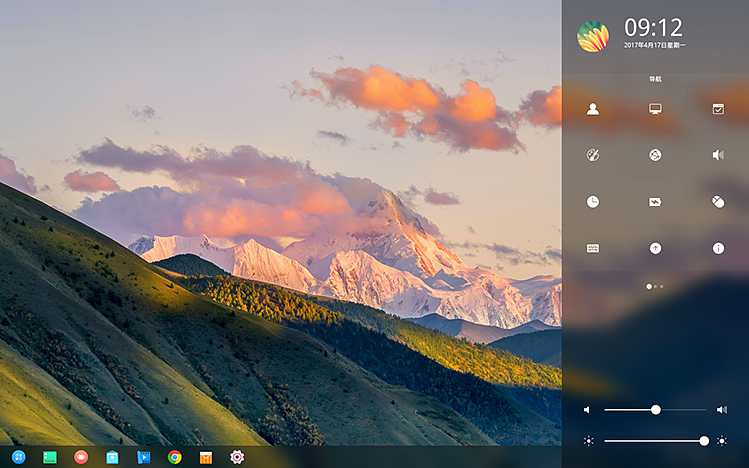
\includegraphics{deepin-desktop-setting-1.jpg}
\captionof{figure}{控制中心}
\label{deepin-desktop-setting}
\end{center}
\end{minipage}}

首页展示快速入口、常用快捷设置等,让操作更加方便和快捷;天气详情、通知中心通过插件展示,今后会开放插件接口,让您可以更多的参与定制。有兴趣的话,可以点开逐步试试。

\subsection{开机自启动}

一些软件需要开机自启动,比如 QQ 还有一些保护眼睛的软件,比如定时休息的
workrave, 减少蓝光的 red-shift。点击
\textbf{Super}键,弹出所有的软件图标,看中要开机自启动的,右击选择开机启动。

\leftline{\begin{minipage}{\linewidth}
\begin{center}
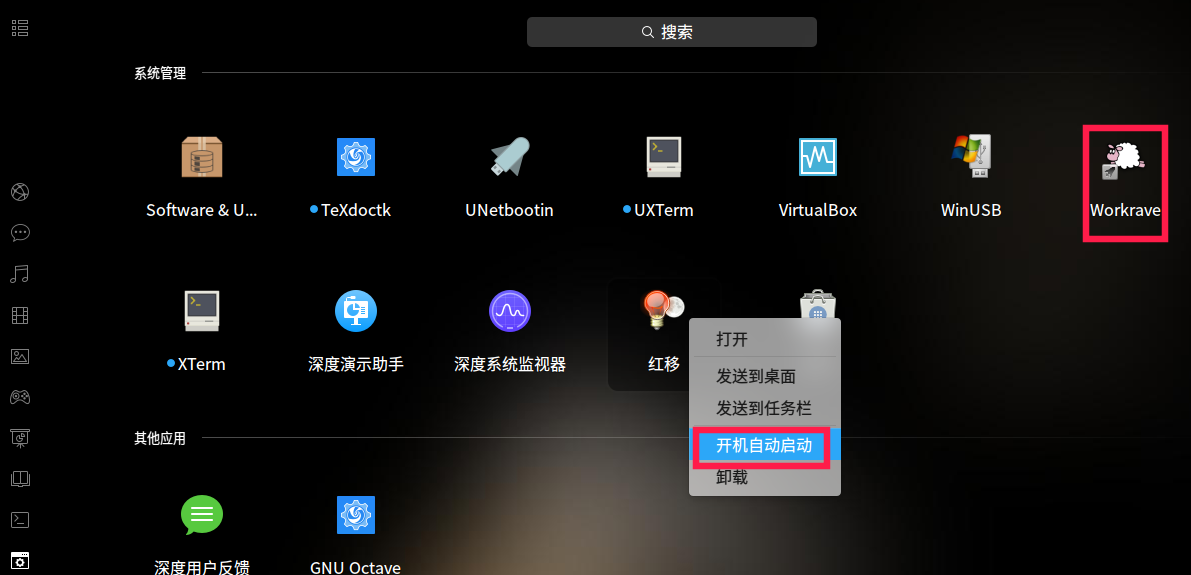
\includegraphics{boot-auto.png}
\captionof{figure}{开机自启动}
\label{boot-auto}
\end{center}
\end{minipage}}

\subsection{常用快捷键}

常用快捷键类似微软 Windows
操作系统,还可以自己定制快捷键。详情请参考\textbf{控制中心} \(->\)
\textbf{键盘和语言} \(->\) \textbf{快捷键}。

\subsection{安装软件}

使用电脑,不可避免的要用到很多软件。深度商店为您解忧愁,方便您查找并安装相关的软件。当然除了深度商店,您还可以使用命令行安装软件,关于命令行安装软件的介绍详见后面章节。

\leftline{\begin{minipage}{\linewidth}
\begin{center}
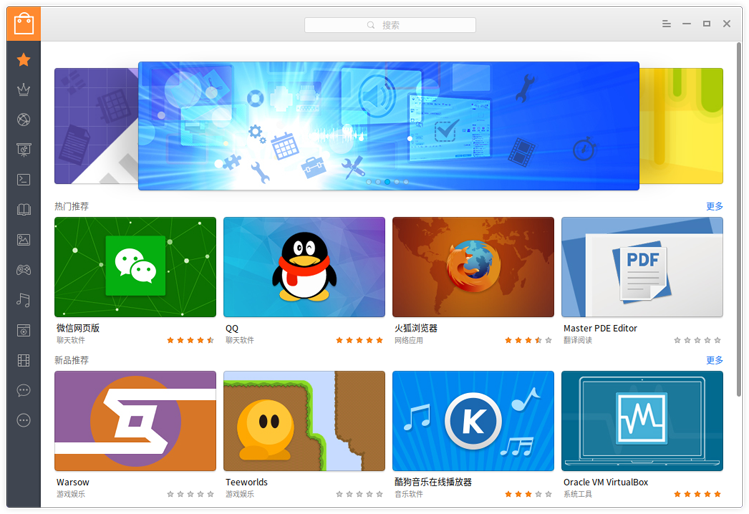
\includegraphics{deepin-store-1.png}
\captionof{figure}{深度商店}
\label{deepin-store}
\end{center}
\end{minipage}}

\subsection{卸载软件}

按 windows
键,弹出的软件,右击选择卸载。或者命令行,这里就不介绍了,在后面详细说明。

\section{深度桌面常用软件}

打开深度商店,会有很多常用软件推荐,另外在官网\href{https://www.deepin.org/original/}{深度原创应用}有深度大量原创好用的软件,在官网\href{https://www.deepin.org/cooperative/}{深度合作应用}等也有几个非常杰出的软件,下面介绍几款。

\subsection{搜狗输入法}

这个是系统默认自带的了,贴它是为了怀念曾经被输入法折磨的岁月。官网有详细介绍:\url{http://pinyin.sogou.com/linux/?r=pinyin}

不过我最希望有讯飞语音输入法,这个如果可以在 Linux
桌面下生存,是最好不过的。不过当前还没有 Linux 版本。

\hypertarget{qq}{%
\subsection{QQ}\label{qq}}

国人挚爱。可以视频。就不废话了。系统默认自带,如果没有,命令行安装。

\begin{lstlisting}[language=bash]
$ sudo apt-get update
$ sudo apt-get install deepin.com.qq.im
\end{lstlisting}

\subsection{深度截图}

深度截图是深度科技团队开发的一款精巧截图应用,它具有智能窗口识别、快捷键支持、图片编辑、延迟截图、智能保存、调节图像分辨率等功能。

\leftline{\begin{minipage}{\linewidth}
\begin{center}
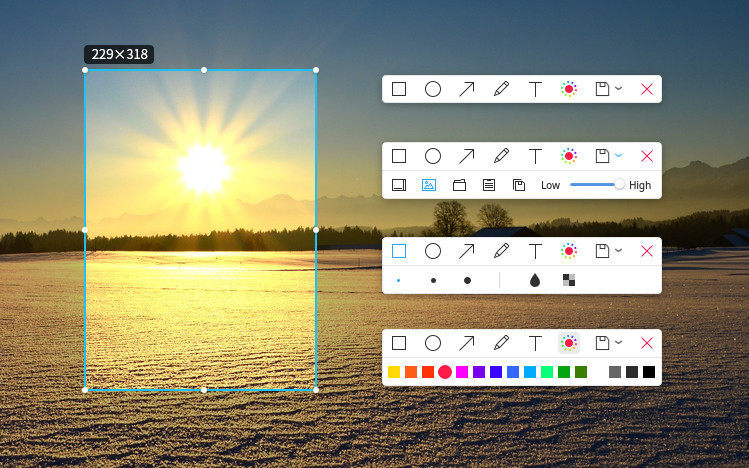
\includegraphics{deepin-screenshot-3.jpg}
\captionof{figure}{深度截图中文版}
\label{deepin-screenshot}
\end{center}
\end{minipage}}

深度截图也是系统默认自带的,如果没有,直接在深度商店搜索下载,也可以采用命令行安装。

\begin{lstlisting}[language=bash]
$ sudo apt-get install deepin-screenshot
\end{lstlisting}

\subsection{网易云音乐}

为了带来更好的音乐体验,实现对音乐高品质的追求,经过网易云音乐与深度科技团队长达半年多的联合开发,大家期待已久的网易云音乐正式登陆Linux平台!

\leftline{\begin{minipage}{\linewidth}
\begin{center}

\includegraphics{netease-cloud-music-3.jpg}
\captionof{figure}{网易云音乐}
\label{netease-cloud-music}
\end{center}
\end{minipage}}

深度操作系统用户可运行深度商店,搜索\cqh 网易云音乐
\cqt 进行安装体验,非深度操作系统用户可前往网易云音乐官网下载Linux客户端安装体验。另外,您也可以命令行安装。

\begin{lstlisting}[language=bash]
$ sudo apt-get install netease-cloud-music
\end{lstlisting}

\subsection{深度系统监视器}

深度系统监视器是深度科技团队打造一款直观易用的系统监视器应用,它可以实时监控处理器状态、内存占用率、网络上传下载速度;还可以管理您的系统进程和应用进程,支持搜索进程和强制结束进程。

\leftline{\begin{minipage}{\linewidth}
\begin{center}
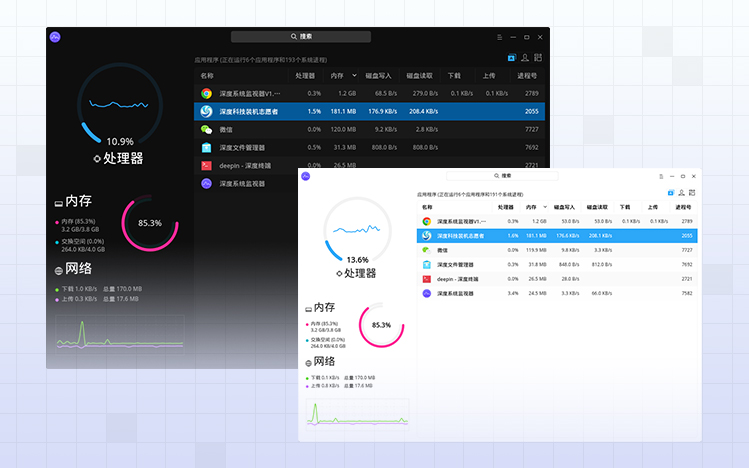
\includegraphics{deepin-system-monitor-2.jpg}
\captionof{figure}{深度系统监视器}
\label{deepin-system-monitor}
\end{center}
\end{minipage}}

系统默认自带,如果没有,可以深度商店搜索下载,也可命令行安装。

\begin{lstlisting}[language=bash]
$ sudo apt-get install deepin-system-monitor -y
\end{lstlisting}

\subsection{深度无线投屏}

深度演示助手是一款用于手机内容分享的演示工具。它支持照片分享功能,分享时可以对照片进行旋转、标记、聚焦等操作。甚至还可以直接将手机屏幕投射到电脑上,视频、游戏都轻松分享。另外还支持幻灯片远程控制,让您在演示幻灯片时无拘无束。

\leftline{\begin{minipage}{\linewidth}
\begin{center}

\includegraphics{deepin-presentation-assistant-1.png}
\captionof{figure}{深度无线投屏}
\label{deepin-presentation-assistant}
\end{center}
\end{minipage}}

系统默认自带,如果没有,可以深度商店搜索下载,也可命令行安装。

\begin{lstlisting}[language=bash]
$ sudo apt-get install deepin-presentation-assistant -y
\end{lstlisting}

\hypertarget{-2}{%
\section{总结}\label{-2}}

本章简要介绍了深度科技公司及深度操作系统的部分内容,并对桌面常用的一些操作和常用的若干软件做了简单描述。如果需要对深度操作系统的框架了解更多,可以阅读官网\href{https://www.deepin.org/developer-community/architectural-design/}{架构设计},或者更进一步阅读\href{https://github.com/linuxdeepin}{源代码}。

\section{附注}

有建议说要转载王勇的文章,有机会试试。

\hypertarget{chap:education-intro}{%
\chapter{教学用的 Linux 软件}\label{chap:education-intro}}

参考网页:

\begin{itemize}
\tightlist
\item
  \url{https://www.linux.com/news/best-linux-tools-teachers-and-students}
\item
  \url{https://linux.cn/article-9722-1.html}
\end{itemize}

\section{引言}

邓公当年曾说``计算机的普及要从娃娃做起。''其实深度操作系统的普及也可以从娃娃抓起。电脑的应用,更多的在于顺手的软件,教育方面也不例外。本章参考网上部分资料,介绍一些方便教学的软件。

\section{笔记}

毛主席的一个读书习惯``不动笔墨不读书'',既然要学习肯定是要做笔记的。GNU/Linux
操作系统下的笔记还是有很多种的,比如\href{http://www.wiz.cn/}{为知笔记}、\href{http://leanote.org/}{leanote}、\href{http://www.qownnotes.org/}{QOwnNotes}、\href{http://basket.kde.org}{BasKet
Note
Pads}、深度官方使用的\href{https://shimo.im/}{石墨文档}等,更多软件可以参考深度商店的\textbf{办公学习}软件列表。当然也有一些便笺软件,比如
Xpad 。读者可以根据自己情况选择需要的软件,下面以 leanote 和 Xpad
为例进行介绍。

\hypertarget{leanote}{%
\subsection{leanote}\label{leanote}}

\passthrough{\lstinline!leanote!} 又称蚂蚁笔记,在深度商店里搜索
\passthrough{\lstinline!leanote!},
如下图\ref{fig:leanote-install}所示,点击安装,等待安装完成,点击打开即可。

\begin{figure}

{\centering 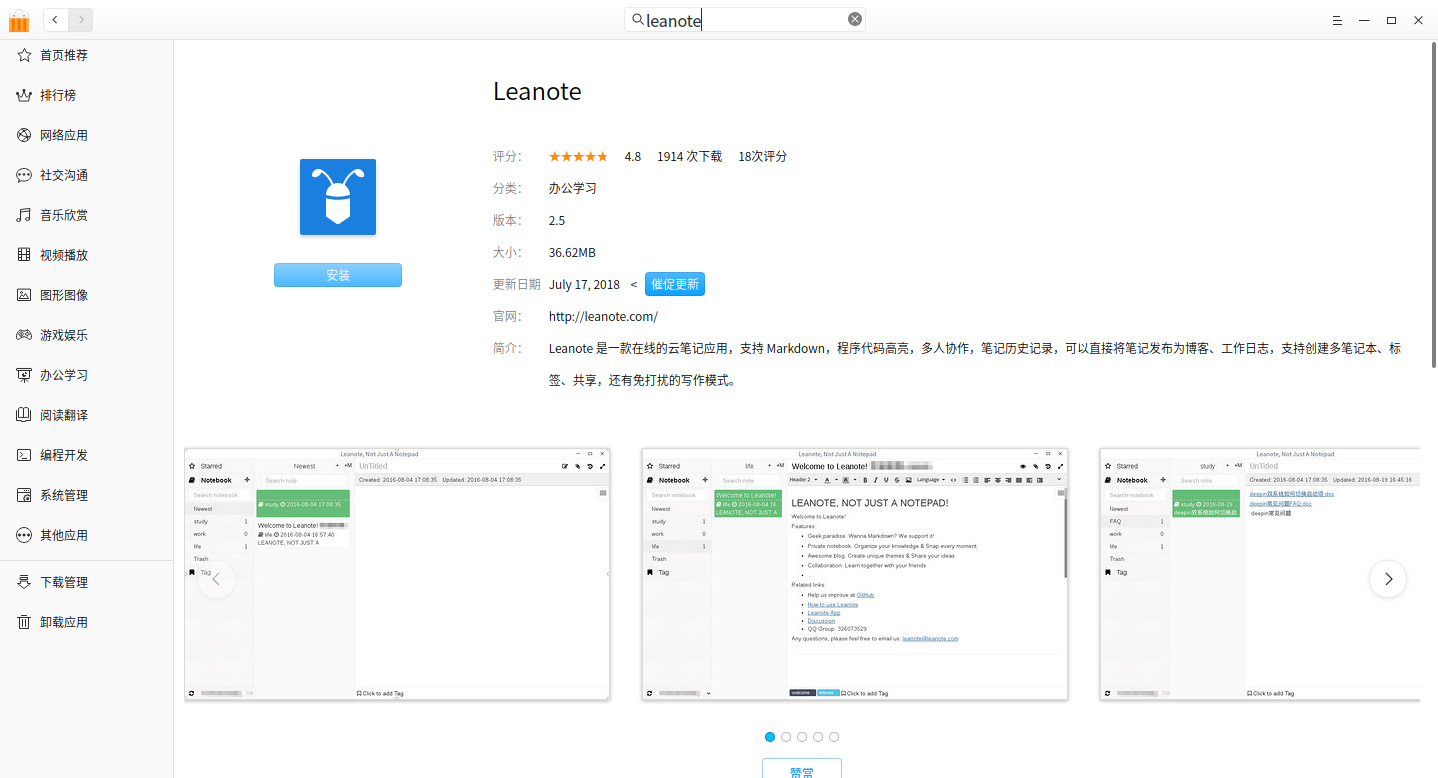
\includegraphics[width=1\linewidth]{images/education-leanote-install} 

}

\caption[leanote 软件安装]{leanote 软件安装}\label{fig:leanote-install}
\end{figure}

安装完成后,注册登录,就可以使用了。本人试用界面如图\ref{fig:leanote-use}。该笔记软件跟其他很多笔记软件类似,可以离线在线使用,甚至自建服务器。能够满足日常需要了。

\begin{figure}

{\centering 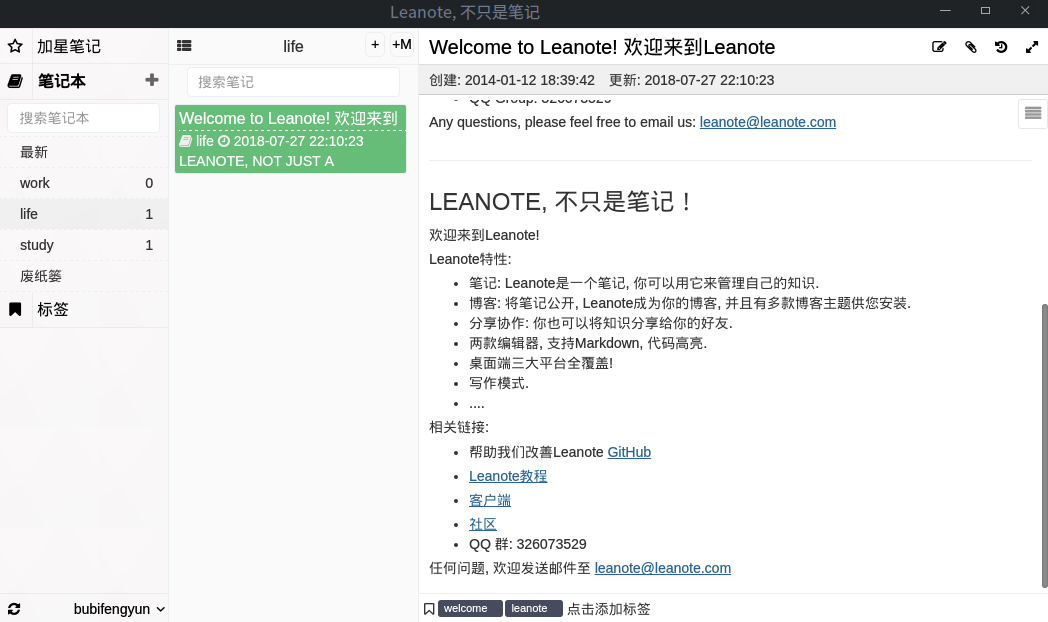
\includegraphics[width=1\linewidth]{images/education-leanote-use} 

}

\caption[leanote 使用界面]{leanote 使用界面}\label{fig:leanote-use}
\end{figure}

\hypertarget{xpad-}{%
\subsection{Xpad 便笺}\label{xpad-}}

在深度商店里搜索
\passthrough{\lstinline!xpad!},找到该软件,点击安装即可。安装成功后,按下
\passthrough{\lstinline!win!}
键或者鼠标点击左下角\textbf{启动器}按钮,弹出软件列表界面。如图\ref{fig:xpad-smallscreen}
或者 图\ref{fig:xpad-fullscreen}所示

\begin{figure}

{\centering 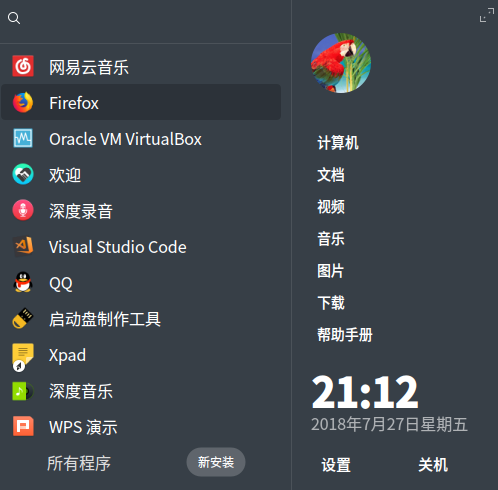
\includegraphics[width=0.618\linewidth]{images/education-xpad-search-smallscreen} 

}

\caption[小号版软件列表]{小号版软件列表}\label{fig:xpad-smallscreen}
\end{figure}

\begin{figure}

{\centering 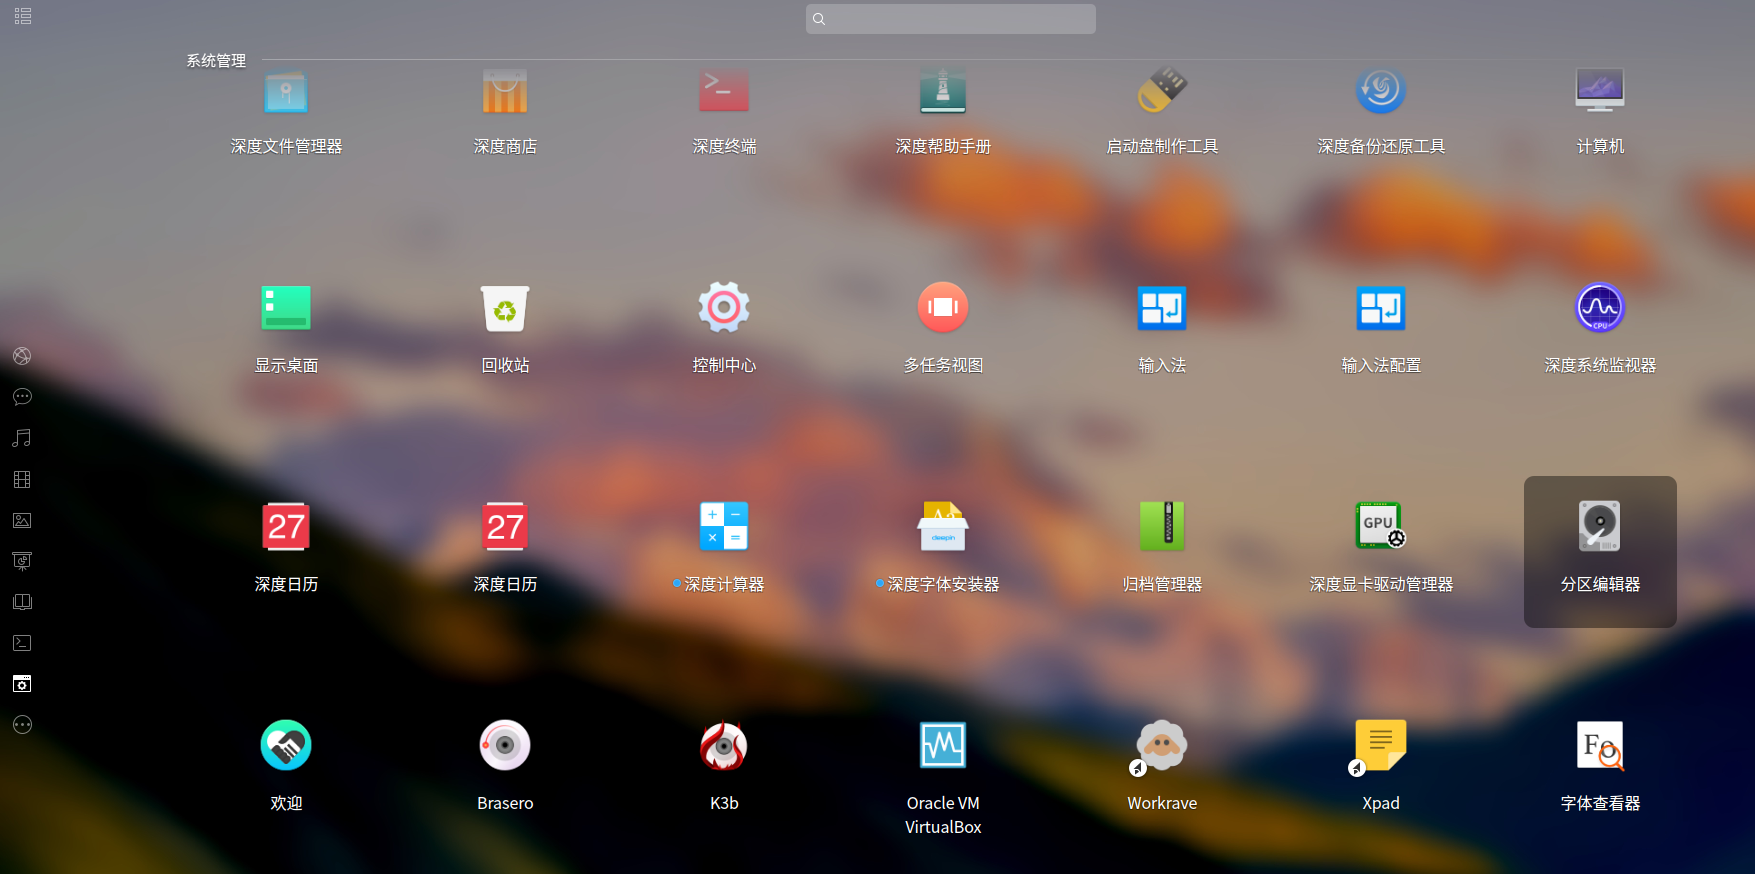
\includegraphics[width=1\linewidth]{images/education-xpad-search-fullscreen} 

}

\caption[全屏版软件列表]{全屏版软件列表}\label{fig:xpad-fullscreen}
\end{figure}

在上述界面中,都有搜索框,可以在搜索框里输入
\passthrough{\lstinline!xpad!}
查找。找到后,点击图标,就会打开类似图\ref{fig:xpad-start}的界面,跟
win7 便签很类似。

\begin{figure}

{\centering 
\includegraphics[width=0.618\linewidth]{images/education-xpad-start} 

}

\caption[Xpad 初始界面]{Xpad 初始界面}\label{fig:xpad-start}
\end{figure}

Xpad
初始界面不一定符合用户习惯,可以自定义配置。在界面上右击,会弹出如图\ref{fig:xpad-rightclick}列表,选择\textbf{Preferences}(首选项),进行配置。

\begin{figure}

{\centering 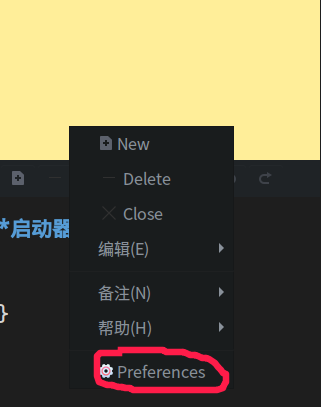
\includegraphics[width=0.618\linewidth]{images/education-xpad-rightclick} 

}

\caption[Xpad 右键列表]{Xpad 右键列表}\label{fig:xpad-rightclick}
\end{figure}

为了方便,对弹出的界面图\ref{fig:xpad-setwin},我做了如下配置,勾选了\textbf{View
\textgreater{}\textgreater{} Show Window Decorations}用于显示窗口,以及
\textbf{Startup \textgreater{}\textgreater{} Start Xpad automatically
after login}开机自启动。

\begin{figure}

{\centering 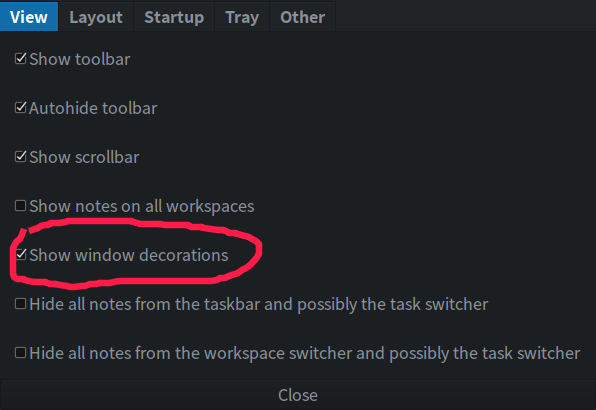
\includegraphics[width=0.618\linewidth]{images/education-xpad-setwin} 

}

\caption[Xpad 配置页面]{Xpad 配置页面}\label{fig:xpad-setwin}
\end{figure}

如果需要删除某个便签,选中按下 \textbf{Shift + Delete} 键即可。

\section{课堂工具}

对于课堂工具,本章主要介绍师生屏幕广播软件,功能类似 Windows 下的
\textbf{红蜘蛛多媒体网络教室软件}以及。

\hypertarget{veyon}{%
\subsection{Veyon}\label{veyon}}

该软件\href{https://github.com/veyon/veyon/}{开源},\href{https://veyon.io/}{官网}能够下载
Window 和 Linux
版本的\href{https://veyon.io/download/}{安装包}。主要功能允许教师查看学生桌面上发生了什么,控制他们的桌面,锁定他们的桌面,对桌面演示,打开或关闭桌面,向学生桌面发送文本消息等等。安装方式如下,

\begin{lstlisting}[language=bash]
$ sudo apt-get install veyon -y
\end{lstlisting}

具体使用方法,请参考\href{https://veyon.io/docs/}{官网文档}或者网上搜索相关资料。

\hypertarget{acontent}{%
\subsection{AContent}\label{acontent}}

AContent 是 \href{https://github.com/atutor?tab=repositories}{aTutor}
的一个加强包,能够创建和管理在线考试和测验,分享教学资料等。

\begin{itemize}
\tightlist
\item
  \href{https://atutor.github.io/acontent/downloads.html}{下载地址}
\item
  \href{https://github.com/atutor/AContent}{github源码}
\end{itemize}

安装方法从略。使用有一定难度,不是太推荐。

\hypertarget{moodle}{%
\subsection{Moodle}\label{moodle}}

比较推荐这个,这是一个网站,需要预先安装服务器,比如 Apache,MySQL
等,为了方便可以使用一键安装软件 XAMPP 等。

\begin{itemize}
\tightlist
\item
  \href{https://moodle.org/}{官网}
\item
  \href{https://github.com/moodle/moodle}{github源码}
\item
  \href{https://baike.baidu.com/item/moodle}{百度百科}
\end{itemize}

其官网有相关说明,需要一定的网页技术知识,这里不赘述了。

\section{文献阅读写作管理工具}

对于学生和部分秉承``活到老学到老''精神的人来说,好的文献阅读工具必不可少。同样一些方便写作的编辑器也是很有市场的。对于
word 文档,比如金山 WPS
旗下产品或者永中等已经很多了,这里就不介绍了。对于程序员``编辑器之神''
vim 和``神之编辑器''emacs
的争论也未曾停息。这里简要介绍几款论文写作的工具。

\textbf{如果有更好的软件,或者使用方法,也请读者不吝赐教,感谢。}

\hypertarget{bookdown}{%
\subsection{bookdown}\label{bookdown}}

参考网页:

\begin{itemize}
\tightlist
\item
  \url{https://bookdown.org/yihui/bookdown/}
\end{itemize}

Bookdown 基于 \href{http://rmarkdown.rstudio.com}{R
Markdown},具有Markdown语法的简单性(您可以在5分钟内学习基础知识;参见附录\ref{chap:rmarkdown}),提供多种输出格式(PDF/HTML/Word/\ldots{})。还添加了多页HTML输出、编号和交叉引用图形/表格/部分/方程、插入部分/附录等特性,支持\href{https://www.gitbook.com}{GitBook样式}便于创建优雅和吸引人的HTML图书页面。

尽管Bookdown包含``书''(book)一词,但不限于生成书籍,也可以生成课程讲义、学习笔记、软件手册、论文,甚至日记等。

另外,班门弄斧一下,本书就是采用
\href{https://github.com/bubifengyun/deepin-bible}{bookdown
模板}编写的,自认为还是有点精美的。另外本人制作了\href{https://github.com/bubifengyun/SJTUThesis-Rmd}{上海交大论文模板},也有好事者\href{https://github.com/pzhaonet/bookdownplus}{赵鹏}移植了若干模板,有兴趣把各高校论文
\LaTeX 模板改为 bookdown 的,可以共同讨论。

\hypertarget{vufind}{%
\subsection{VuFind}\label{vufind}}

参考网页:

\begin{itemize}
\tightlist
\item
  \url{https://www.oschina.net/p/vufind}
\item
  \url{http://vufind.org/}
\end{itemize}

VuFind
是图书馆资源门户系统,主要提供图书馆资源的检索和浏览功能,功能模块包括:

\begin{itemize}
\tightlist
\item
  Catalog Records
\item
  Locally Cached Journals
\item
  Digital Library Items
\item
  Institutional Repository
\item
  Institutional Bibliography
\item
  Other Library Collections and Resources
\end{itemize}

VuFind 是完全模块化的,你可以自由选择模块。全平台支持,当然包括
Linux,二进制文件\href{https://vufind.org/vufind/downloads.html}{官网}提供下载。

\hypertarget{calibre}{%
\subsection{Calibre}\label{calibre}}

参考网页:

\begin{itemize}
\tightlist
\item
  \url{https://calibre-ebook.com/}
\item
  \url{https://calibre-ebook.com/download_linux}
\end{itemize}

Calibre 是电子书管理软件,支持 Amazon、Apple、Bookeen、Ectaco、Endless
Ideas、Google/HTC、Hanlin Song
设备及格式,功能十分强大。通常我都是按照官网提供的方法下载安装

\begin{lstlisting}[language=bash, numbers=none]
$ sudo -v && wget -nv -O- \
https://download.calibre-ebook.com/linux-installer.sh \
| sudo sh /dev/stdin
\end{lstlisting}

\hypertarget{cajviewer}{%
\subsection{CAJViewer}\label{cajviewer}}

参考网页:

\begin{itemize}
\tightlist
\item
  \url{http://cajviewer.cnki.net/introduction.html}
\end{itemize}

``CAJViewer 7.2'' 是光盘国家工程研究中心、清华同方知网(北京)技术有限公司
CAJViewer 系列产品截至 2006 年 11
月为止的最新版本,它充分吸取了当前市场上各种同类主流产品和自身上一版本
CAJViewer 6.0 的优点,经过长时间市场调查和系统设计而成,兼容 CAJ 和 PDF
等文件。

对于高校学生,这个阅读器你懂得。深度提供了相应版本。

\hypertarget{-everything}{%
\subsection{搜索神器 Everything}\label{-everything}}

参考网页:

\begin{itemize}
\tightlist
\item
  \url{http://www.voidtools.com/}
\item
  \url{http://www.voidtools.com/downloads/}
\item
  \url{https://github.com/DoTheEvo/ANGRYsearch}
\end{itemize}

\begin{quote}
Everthing
正是当之无愧的最强文件搜索神器!!它可以在闪电般的瞬间从海量的硬盘中找到你需要的文件!速度快到绝对让你难以置信!首次接触到
Everything
可真让我惊讶和兴奋了许久!!而且它还是一款完全免费的软件,界面简洁高效,体积很小巧,但功能却非常丰富!Everything
文件搜索工具最大的优点是近乎变态的速度。其速度不是快,是快到离谱;用户不是满意,而是震惊。你甚至会愤怒,它凭什么这么快?!

\VA{--- \href{https://www.iplaysoft.com/everything.html}{Everything 用户}}{}
\end{quote}

当然这个 Everything 目前只能用于 Windows
系统。在深度下也有类似的软件,ANGRYsearch。如果感兴趣的不妨试试。\href{https://github.com/DoTheEvo/ANGRYsearch}{源码}有安装说明。

\partquote{竹外桃花三两枝,春江水暖鸭先知}{苏轼}
\partintro{
GNU/Linux 领域也可以说是博大精深,仿佛一江春水,作为初入门庭的小白,暂且从命令行、文件系统、文本处理等方面试试水吧。待轻车熟路后,相信诸位一定能够如龙入海,纵横驰骋在这片快捷高效的领域里。
}

\hypertarget{part:basic}{%
\part{GNU/Linux 基础知识}\label{part:basic}}

\hypertarget{chap:shell}{%
\chapter{shell 用法简介}\label{chap:shell}}

通过阅读本章,你将会了解到以下几项内容。

\begin{itemize}
\tightlist
\item
  了解 Linux Shell
\item
  打开 Shell 终端的方法
\item
  Bash 语法简介
\item
  Bash 自动补全和输入历史
\item
  命令的拼接和拓展
\item
  变量和简写
\item
  如何使用理解帮助文档
\end{itemize}

作为普通人,使用电脑除了窗口图形界面外,还有个叫终端的字符界面。Linux
中通过在终端敲击字符跟电脑交互,这玩意就叫做
shell,并且相比图形界面(Graphic User Interfaces, GUI),通常 shell
功能更加强大。

深度系统默认采用的 shell\index{shell}是
\passthrough{\lstinline!bash!}(Bourne Again Shell),继承兼容于 UNIX
早期的 Bourne shell (作者:Stephen Bourne, 命令名为
\passthrough{\lstinline!sh!}),当然两者还是有那么一点点不同的。曾经有一段时间深度默认
shell 是 \passthrough{\lstinline!zsh!},经群众投票又改回
\passthrough{\lstinline!bash!}了,其实\href{https://bbs.deepin.org/forum.php?mod=viewthread\&tid=30976\&extra=}{那次投票}是我发起的。

除此之外,类 UNIX 系统还有其他的一些 shell,比如
\passthrough{\lstinline!ksh!},\passthrough{\lstinline!csh!},\passthrough{\lstinline!tcsh!},\passthrough{\lstinline!ash!},当然还有非常好用的
\passthrough{\lstinline!zsh!} 等,有兴趣的可以查相关资料。

\hypertarget{-shell-}{%
\section{用 shell 有啥好处?}\label{-shell-}}

为了装吗?不见得。

刚接触 Linux 桌面发行版的时候,按着教材说的,就在学习终端哦。遇到糟糕的
Linux 图形界面卡住了、死机啦,不得不网上搜索解决方案,能不用终端 shell
吗?作为小白,遇到各种各样的问题,查询询问的结果,大神的建议,也多半是在
shell 下解决啊,这叫不得不用。

后来慢慢脱离低级小白,开始喜欢上终端远程连接其他 Linux
电脑,享受这种快捷方便的操作。再后来终端下用 vim
写代码,键盘翻飞,似乎成为了一种享受。

再后来,开始接管一些服务器,开始学习计算机安全知识,似乎更离不开了 shell
了。似乎儿时那种黑客的感觉,只有通过 shell 才可以实现哦。

其实 Windows 下也有 DOS 和 CMD 这类字符操作界面,不过功能弱爆了,
powershell 可能功能强大一些,有兴趣的可以查相关资料,这里不说了。

\hypertarget{shell:intro}{%
\section{深度操作系统下 shell 简介}\label{shell:intro}}

按照《Linux Bible》的说法,有三种方式打开 shell
操作界面,分别叫shell提示符(shell
prompt)\index{shell},终端窗口(Terminal
window),和虚拟控制台(virtual
console)。我感觉深度操作系统就后面两种,第一种说是登录的时候出现的那种字符界面,不太容易遇到,暂且跳过。

深度操作系统登录后,进入桌面,按下
\passthrough{\lstinline!Ctrl + Alt + T!}
(或\passthrough{\lstinline!F4!}或\passthrough{\lstinline!Alt + F2!}打开终端雷神模式,这个版本不同有所变化)会弹出深度终端窗口,这个软件在第三章已经作了介绍。可用于
shell\index{shell} 练习。对于虚拟控制台,可以通过按下
\passthrough{\lstinline!Ctrl + Alt + Fi!} 其中
\passthrough{\lstinline!Fi!} 表示
\passthrough{\lstinline!F1,F2,...,F6!},分别弹出六个虚拟控制台,对于不同的电脑,可能\passthrough{\lstinline!Ctrl + Alt + F1!}
或者\passthrough{\lstinline!Ctrl + Alt + F7!} 打开的是图形界面(GUI)。

下面以深度终端窗口为例来说明。

\textbf{打开深度终端的方式}

\begin{itemize}
\tightlist
\item
  快捷键的方式:按下 \passthrough{\lstinline!Ctrl + Alt + T!} 或者
  \passthrough{\lstinline!F4!} 或
  \passthrough{\lstinline!Alt + F2!},弹出深度终端。
\item
  图形方式:按下 \passthrough{\lstinline!super!}
  键,或者点击左下角的图标,会弹出已安装软件图标,找到深度终端的图标,点击即可。或者在最上面搜索框中搜索终端。
\item
  鼠标右键:在桌面上,右击选择在终端中打开,也可以进入深度终端。
\end{itemize}

打开终端后,右击窗口内部,选择设置,可以对终端的一些外观属性配置。

\textbf{深度终端的显示说明}

在每行命令行开头会如下显示,

\begin{lstlisting}[language=bash]
litianci@litianci-pc:~$ 
\end{lstlisting}

\textbf{解释}

\begin{enumerate}
\def\labelenumi{\arabic{enumi}.}
\tightlist
\item
  \passthrough{\lstinline!litianci@litianci-pc:\~!}
  表示用户名和电脑名,并用\passthrough{\lstinline!@!}隔开,\passthrough{\lstinline!:!}后是当前工作目录\passthrough{\lstinline!~!},\passthrough{\lstinline!~!}是主目录的意思,因为古老的键盘中\passthrough{\lstinline!~!}和\passthrough{\lstinline!Home!}是同一个按键,所以就用
  \passthrough{\lstinline!\~!}代替主目录了。
\item
  \passthrough{\lstinline!$!} 默认表示普通用户,
  \passthrough{\lstinline!#!} 默认表示 root 根用户。
\item
  这个显示说明是可以修改的,见后文 @ref() 小节。
\item
  在 \passthrough{\lstinline!$!} 或者 \passthrough{\lstinline!#!}
  后输入相关的命令字符。
\end{enumerate}

\passthrough{\lstinline!$!} 表示正在用普通用户权限运行后面的命令,而
\passthrough{\lstinline!#!} 则表示正在使用 root
根用户的权限。通常只有涉及重大核心系统功能的地方才需要用到root根用户权限。根据放权的最小权限原则,在普通用户权限可做的事情,建议不要使用
root 根用户权限。

\subsection{牛刀小试}

下面命令行首标志 \passthrough{\lstinline!$!} 和
\passthrough{\lstinline!#!}
区分运行权限,其他显示信息略。输入结果行没有行首标志,每行会有序号方便区分。

\begin{lstlisting}[language=bash]
$ whoami
litianci
$ who -H
名称   线路       时间           备注
litianci tty1         2018-09-20 09:07 (:0)
$ grep litianci /etc/passwd
litianci:x:1000:1000::/home/litianci:/bin/bash
\end{lstlisting}

\textbf{解释}

\begin{enumerate}
\def\labelenumi{\arabic{enumi}.}
\tightlist
\item
  \passthrough{\lstinline!whoami!} 列出当前用户名
\item
  \passthrough{\lstinline!who -H!}
  列出信息更详细,\passthrough{\lstinline!-H!}
  表示显示头部标题列,第二行显示当前登录用户名\passthrough{\lstinline!litianci!},当前登录线路终端\passthrough{\lstinline!tty1!},当前用户登录系统时间\passthrough{\lstinline!2018-09-20 09:07!},以及备注\passthrough{\lstinline!(:0)!},\textbf{该备注啥意思暂时没有找到,是不是图形界面的意思,待后续找资料。}
\item
  第6行,是在\emph{/etc/passwd}文件内查找该用户,在第7行最后\passthrough{\lstinline!/bin/bash!},表示该用户默认的shell类型。实际操作时请把\passthrough{\lstinline!litianci!}换成你的账户名。
\end{enumerate}

\begin{lstlisting}[language=bash]
$ date
2018年 09月 21日 星期五 16:45:08 CST
$ pwd
/home/litianci
$ hostname
litianci-PC
$ hostname -I
192.168.43.45
$ ls
Desktop  Documents  Downloads  Music  Pictures  Videos
\end{lstlisting}

\textbf{解释}

\begin{enumerate}
\def\labelenumi{\arabic{enumi}.}
\tightlist
\item
  \passthrough{\lstinline!date!}
  命令,无选项无参数时,输出当前日期、星期、时间和时区。其中CST表示中国标准时区,也即东八区。不过CST这个简写有\href{https://blog.csdn.net/sjpljr/article/details/70169056}{歧义},代表如下几个时区,

  \begin{itemize}
  \tightlist
  \item
    CST Central Standard Time (USA) UT-6:00
  \item
    CST Central Standard Time (Australia) UT 9:30
  \item
    CST China Standard Time UT 8:00
  \item
    CST Cuba Standard Time UT-4:00
  \end{itemize}
\item
  \passthrough{\lstinline!pwd!} 命令输出当前工作目录。
\item
  \passthrough{\lstinline!hostname!}
  命令,无选项无参数时输出本机名称,如果加选项\passthrough{\lstinline!-I!},则输出本机IP地址。
\item
  \passthrough{\lstinline!ls!}
  命令列出当前目录下所有的可见文件及文件夹。
\end{enumerate}

\subsection{命令语法结构}

为了丰富命令的功能,命令常常带多种选项及参数的,\href{https://www.jb51.net/os/RedHat/518485.html}{这里}区分两个名称,

\begin{itemize}
\tightlist
\item
  \textbf{选项(Options):}是调整命令执行行为的开关,即,选项不同决定了命令的显示结果不同;
\item
  \textbf{参数(Arguments):}是指命令的作用对象。
\end{itemize}

\hypertarget{options}{%
\subsection{选项(Options)}\label{options}}

选项分为长选项和短选项。下面示例中,\passthrough{\lstinline!-l -a -t!}就是短选项,

\begin{lstlisting}[language=bash]
$ ls -l -a -t
$ ls -lat
\end{lstlisting}

\textbf{解释}

\begin{enumerate}
\def\labelenumi{\arabic{enumi}.}
\tightlist
\item
  \passthrough{\lstinline!-l!}(long
  listing),宽列,较长格式列出信息,\passthrough{\lstinline!-a!}(all)列出所有文件(夹),包括隐藏文件(夹),\passthrough{\lstinline!-t!}(time)按时间排序。
\item
  \textbf{短选项}一般使用\passthrough{\lstinline!-!}短横线引导。也有不带\passthrough{\lstinline!-!}的,比如\passthrough{\lstinline!ps aux!},这类叫BSD风格的选项。
\item
  当有多个短选项时,各选项之间使用空格隔开。
\item
  有些短选项可以组合,比如 \passthrough{\lstinline!-l -a -t!}
  可以组合为\passthrough{\lstinline!-lat!}。
\item
  有些短选项需带参数,比如-L
  512M,则不便跟其他短选项组合,但如果位于最后一个也是可以组合的。比如\passthrough{\lstinline!tar cvf deepin-bible.tar \~/deepin-bible!},各选项说明见后面\ref{shell:more-example}节解释。
\end{enumerate}

\begin{lstlisting}[language=bash]
$ ls --hide=Desktop
Documents  Downloads  Music  Pictures  Videos
\end{lstlisting}

\textbf{解释}

\begin{enumerate}
\def\labelenumi{\arabic{enumi}.}
\tightlist
\item
  \passthrough{\lstinline!--hide=Desktop!},不列出 Desktop 这一文件夹。
\item
  \textbf{长选项}一般使用\passthrough{\lstinline!--!}两个短横线引导,而且后接完整英文单词。
\item
  长选项通常不能组合。
\item
  长选项如果需要参数,一般用\passthrough{\lstinline!=!},比如\passthrough{\lstinline!--size=1G!}。不过也有用空格隔开的,比如
  \passthrough{\lstinline!pandoc test.md --to latex!}表示使用\passthrough{\lstinline!pandoc!}命令把\emph{test.md}文件转化为\passthrough{\lstinline!latex!}格式。
\end{enumerate}

以上均为常见格式,具体使用方法,还需查看相关命令的帮助,比如\passthrough{\lstinline!cmd --help!},获得正确用法。

\hypertarget{arguments}{%
\subsection{参数(Arguments)}\label{arguments}}

上面讲述选项有所介绍,通过空格或者等号传入参数,也有直接通过空格缀在命令后面的。比如,

\begin{lstlisting}[language=bash]
$ cd /media/litianci/data/
\end{lstlisting}

跳转到\emph{/media/litianci/data/} 文件夹。

\hypertarget{shell:more-example}{%
\subsection{更多例子}\label{shell:more-example}}

为了方便大家上手,再多介绍几个例子。

\begin{lstlisting}[language=bash]
$ tar cvf deepin-bible.tar ~/deepin-bible
$ uname
$ uname -a
$ date
$ date +'%Y-%m-%d'
2018-09-21
$ date +'%A, %B %d, %Y'
星期五, 九月 21, 2018
$ id
uid=1000(litianci) gid=1000(litianci) 组=1000(litianci),7(lp),24(cdrom),27(sudo)
$ who -aH
名称     线路       时间           空闲  进程号 备注   退出
           系统引导 2018-09-21 15:54
           运行级别 5 2018-09-21 07:54
litianci + tty1         2018-09-21 07:55  旧��       3820 (:0)
登录     tty2         2018-09-21 21:48             21868 id=tty2
\end{lstlisting}

\textbf{解释}

\begin{enumerate}
\def\labelenumi{\arabic{enumi}.}
\tightlist
\item
  第1行命令,\passthrough{\lstinline!c!}(create)表示创建压缩文件,\passthrough{\lstinline!v!}(verbose)表示详细信息,\passthrough{\lstinline!f!}(file)表示创建的文件为\passthrough{\lstinline!deepin-bible.tar!};这是典型的组合命令,而最后一个组合选项\passthrough{\lstinline!f!}带参数\passthrough{\lstinline!deepin-bible.tar!}。\passthrough{\lstinline!\~/deepin-bible!}置于最后,为待压缩文件夹。这样本条命令实现了对文件夹的压缩。
\item
  第2、3行,\passthrough{\lstinline!uname!}命令,显示系统名字,\passthrough{\lstinline!-a!}(all)选项,表示显示系统所有信息。
\item
  第4、5、7行,输出不同格式的日期时间格式。详细说明可以参考\passthrough{\lstinline!date --help!}的说明。有兴趣的可以多试试。注意系统语言对显示结果的影响。
\item
  第9行,\passthrough{\lstinline!id!},常用于核实自己账户编号信息。
\item
  第11行,\passthrough{\lstinline!-a!}表示显示较多信息,具体信息参考\passthrough{\lstinline!who --help!}说明。\passthrough{\lstinline!-H!}已经在前面说明,显示列标题。
\end{enumerate}

由于采用系统默认的中文,深度终端自作聪明的翻译,有些内容乱码。为了方便叙述,后面把终端显示改为英文的,也即在\emph{\textasciitilde{}/.bashrc}文件加上所用语言选项,并执行。

\begin{lstlisting}[language=bash]
$ echo LANG=en_US >> ~/.bashrc
$ source ~/.bashrc
\end{lstlisting}

或者直接修改所有用户的 bash
信息,\passthrough{\lstinline!sudo gedit /etc/profile!},修改最后一行的\passthrough{\lstinline!LC\_ALL=C!}为\passthrough{\lstinline!LC\_ALL=en!}。

回头再看\passthrough{\lstinline!who -aH!}命令,就清爽了。当然需要你对英文有一定理解了。

\begin{lstlisting}[language=bash]
$ who -aH
NAME       LINE         TIME         IDLE          PID COMMENT  EXIT
           system boot  Sep 21 15:54
           run-level 5  Sep 21 07:54
litianci + tty1         Sep 21 07:55  old         3820 (:0)
LOGIN      tty2         Sep 21 22:02             25289 id=tty2
\end{lstlisting}

\subsection{找找命令文件在哪里}

相信大家都听说过\textbf{一切皆文件}的Unix哲学,其实很多命令都是可执行文件,是可以查看这部分命令的文件的。比如\passthrough{\lstinline!bash!}位于\emph{/bin/bash},那么命令\passthrough{\lstinline!bash!}和\passthrough{\lstinline!/bin/bash!}就是相同的。为啥我们可以简写为
\passthrough{\lstinline!bash!}呢?是因为shell有\passthrough{\lstinline!PATH!}(\textbf{路径})这个环境变量。众多已知目录存放在
\passthrough{\lstinline!PATH!} 变量里,shell
遇到这些没有目录路径的命令,在查找其他默认命令集合无果后,就会去\passthrough{\lstinline!PATH!}路径变量里各目录下去找该文件名,从左到右查找,找到后就执行命令,找不到就会报错。那么你电脑上的
\passthrough{\lstinline!PATH!} 是啥呢?

\begin{lstlisting}[language=bash]
$ echo $PATH
/home/litianci/bin:/usr/local/bin:/usr/bin:/bin:/usr/local/games:/usr/games:/sbin:/usr/sbin
\end{lstlisting}

一般命令,都存放在 \emph{/bin},\emph{/usr/bin},或
\emph{/usr/local/bin} 文件夹。一般管理相关的命令放在 \emph{/sbin} 和
\emph{/usr/sbin} 文件夹,也有一些 GNU/Linux
发行版放在非常规文件夹下。这些文件夹以英文冒号
\passthrough{\lstinline!:!} 隔开。最后无冒号。
而最开始的\emph{/home/litianci/bin}文件夹是自己所用的目录。你可以对
\passthrough{\lstinline!PATH!}
修改,添加某些你常用的命令文件夹。配置方法见后面叙述。

不过这里存在安全隐患,如果罪恶黑客侵入你系统,无权修改你系统级别的文件,但是有能力在你的文件夹下创建可执行文件,比如\emph{/home/litianci/bin},跟系统文件夹的命令同名,你以为你用的是系统的命令,并输入密码,却不料执行的是黑客想要的命令。对于系统管理员,建议输入命令的时候,把目录带全,避免这类权限泄露。

下面总结 shell 查找命令位置的优先级别。

\begin{enumerate}
\def\labelenumi{\arabic{enumi}.}
\tightlist
\item
  别名(aliases)。别名就是某命令包含或不包含一系列选项的集合,便于输入。后面@ref()小节详述。
\item
  shell 保留字(Reserved word),构建 shell
  脚本的基础,比如\passthrough{\lstinline!do!},\passthrough{\lstinline!while!}等。见后面@ref()章详述。
\item
  函数(function),shell 中创建的命令集合。
\item
  shell
  内置命令(built-in),这些命令在文件系统中是找不到的,比如\passthrough{\lstinline!cd!}改变工作目录,\passthrough{\lstinline!exit!}退出shell,\passthrough{\lstinline!echo!}输出文本,\passthrough{\lstinline!history!}查看之前命令运行历史,\passthrough{\lstinline!pwd!}显示当前工作目录,还有\passthrough{\lstinline!set!}和\passthrough{\lstinline!type!}等。
\item
  文件系统中可以执行的文件。比如\passthrough{\lstinline!PATH!}变量中那些目录下的文件等。
\end{enumerate}

\textbf{你输入的命令是哪个呢?}

在 bash 内,使用

\begin{lstlisting}[language=bash]
$ type ls
ls 是 `ls --color=auto` 的别名
\end{lstlisting}

可以看到你的命令是哪个命令。为了显示全部同一名称的命令,可以加\passthrough{\lstinline!-a!}选项。

\begin{lstlisting}[language=bash]
$ type -a ls
ls 是 `ls --color=auto` 的别名
ls 是 /bin/ls
$ type -a cd
cd 是 shell 内建
\end{lstlisting}

可以看到有两个\passthrough{\lstinline!ls!}命令。\passthrough{\lstinline!cd!}是内置命令(翻译有差距)。其他shell也可用\passthrough{\lstinline!which!}命令查找当前正在使用的命令是哪一个。
此外还有可以找命令文件位置的\passthrough{\lstinline!which!}和\passthrough{\lstinline!locate!}(深度系统未自带),有兴趣的可以去找找资料。

\section{命令快捷编辑}

\subsection{方便编辑的快捷键}

如果命令不足够快捷,那还不如鼠标点点点呢。提到编辑器,在 Linux
世界就跳不过编辑器之神(vim)和神之编辑器(emacs)的争论。在这里不探讨孰是孰非。而
bash 默认的编辑方式就是这两者之一的 emacs 模式。如果喜欢 vim
的编辑方式,也可用设置为 vim 模式。在
\emph{\textasciitilde{}/.bashrc}文件末尾加上
\passthrough{\lstinline!set -o vi!},下次启动终端的时候,就是 vi
模式了。所谓模式,也是为了方便编辑,提供一些快捷键等。我最喜欢用的快捷键,就是
\passthrough{\lstinline!Ctrl+A!}跳到行头,\passthrough{\lstinline!Ctrl+E!}跳到行尾和\passthrough{\lstinline!Ctrl+L!}清屏了。其他的都是键盘上下左右键切换,懒得记录这些快捷键。不过还是把这些快捷键列在下面吧。

\begin{longtable}[]{@{}lc@{}}
\caption{光标跳转快捷键说明\label{tab:cmd:skip-shortkey}}\tabularnewline
\toprule
\textbf{快捷键} & \textbf{解释}\tabularnewline
\midrule
\endfirsthead
\toprule
\textbf{快捷键} & \textbf{解释}\tabularnewline
\midrule
\endhead
Ctrl+F & 向前一个字符\tabularnewline
Ctrl+B & 后退一个字符\tabularnewline
Alt+F & 向前一个单词\tabularnewline
Alt+B & 向后一个单词\tabularnewline
Ctrl+A & 跳到该行行首\tabularnewline
Ctrl+E & 跳到该行行尾\tabularnewline
Ctrl+L & 清空屏幕内容\tabularnewline
\bottomrule
\end{longtable}

\textbf{注:}清屏,只是把内容放到屏幕上方,并加入了很大一片空白,滚动鼠标还可以看到刚刚输出的内容。

\begin{longtable}[]{@{}lc@{}}
\caption{编辑快捷键说明\label{tab:cmd:edit-shortkey}}\tabularnewline
\toprule
\textbf{快捷键} & \textbf{解释}\tabularnewline
\midrule
\endfirsthead
\toprule
\textbf{快捷键} & \textbf{解释}\tabularnewline
\midrule
\endhead
Ctrl+D & 删除当前字符\tabularnewline
Backspace & 删除前面字符\tabularnewline
Ctrl+T & 前后字符换位\tabularnewline
Alt+T & 前后单词换位\tabularnewline
Alt+U & 当前单词大写\tabularnewline
Alt+L & 当前单词小写\tabularnewline
Alt+C & 选中字符大写\tabularnewline
Ctrl+V & 插入特殊字符\tabularnewline
\bottomrule
\end{longtable}

\textbf{注:}每个快捷键具体动作,还需要多加练习记忆。对于插入特殊字符的,\passthrough{\lstinline!Ctrl+V!}比如插入表格键\passthrough{\lstinline!Table!},则\passthrough{\lstinline!Ctrl+V+Tab!},经测试不是那么回事。

\begin{longtable}[]{@{}ll@{}}
\caption{复制粘贴快捷键说明\label{tab:cmd:xc-shortkey}}\tabularnewline
\toprule
\textbf{快捷键} & \textbf{解释}\tabularnewline
\midrule
\endfirsthead
\toprule
\textbf{快捷键} & \textbf{解释}\tabularnewline
\midrule
\endhead
Ctrl+K & 剪切光标到行尾的全部字符,含光标所在字符\tabularnewline
Ctrl+U & 剪切光标到行首的全部字符,不含光标所在字符\tabularnewline
Ctrl+W & 剪切光标前到当前单词词首的字符,不含光标\tabularnewline
Alt+D & 剪切光标后到当前单词词尾的字符,含光标\tabularnewline
Ctrl+Y & 粘贴到光标前\tabularnewline
Alt+Y & 循环显示刚刚剪切的内容,待你确定粘贴对象\tabularnewline
Ctrl+C & 删除整行\tabularnewline
\bottomrule
\end{longtable}

\subsection{重输之前的命令}

参考网页:

\begin{itemize}
\tightlist
\item
  \url{https://blog.csdn.net/maplesky2017/article/details/78389068}
\item
  \url{https://www.cnblogs.com/5201351/articles/4208509.html}
\end{itemize}

bash
是会记录你已经输入命令的。使用\passthrough{\lstinline!history!}命令,可以查看相关内容。常见用法如下。

\begin{itemize}
\tightlist
\item
  上下键查看以前的命令(包括\passthrough{\lstinline!Ctrl+N!}、\passthrough{\lstinline!Ctrl+P!}快捷键);
\item
  \passthrough{\lstinline!history 8!} 查看最近八条命令记录;
\item
  \passthrough{\lstinline!history!}
  查看最近\passthrough{\lstinline!$HISTSIZE!}条命令记录
\item
  \passthrough{\lstinline"!n"} 调用第n条命令,n是一个正整数;
\item
  \passthrough{\lstinline"!!"} 调用上一条命令;
\item
  \passthrough{\lstinline"!字符串"} 调用最后一以该字符串开头的命令。
\end{itemize}

本人感觉以上命令不太实用。除非你知道刚刚是啥命令,才方便操作。Matlab
软件的命令记录就很好查询。输入部分字符就可以把所有以该字符开头的命令记录一次列出。对于
bash,类似的功能非常鸡肋。在空行内按下快捷键\passthrough{\lstinline!Ctrl+R!},输入部分字符,会查找相关命令记录,符合你需求,回车,就直接运行了。丝毫不给你重新编辑的机会,也无法上下翻阅,难用至极。另外还有快捷键\passthrough{\lstinline!Ctrl+S!}在深度操作系统下,不能用。另外两个\passthrough{\lstinline!Alt+P!},\passthrough{\lstinline!Alt+N!}有心情的可以试试。如果哪位有好的用法,欢迎提供。

默认记录1000条命令,但是事实上记录文件里记录的命令条数可能超过此数值。可以输入如下命令查看,

\begin{lstlisting}[language=bash]
$ echo $HISTSIZE
1000
$ echo $HISTFILE
/home/litianci/.bash_history
\end{lstlisting}

\textbf{解释}

\begin{enumerate}
\def\labelenumi{\arabic{enumi}.}
\tightlist
\item
  第1行命令,查询命令记录条数,显示为1000。变量\passthrough{\lstinline!$HISTSIZE!}用于设置记录条数。
\item
  第3行命令,查看命令记录文件,本机为\emph{/home/litianci/.bash\_history}。
\end{enumerate}

如果我们想修改记录条数,或者记录文件,可以\emph{/etc/profile}修改相应的变量。下面以修改记录条数为200进行讲解。

\begin{lstlisting}[language=bash]
$ sudo sed -i 's/^HISTSIZE=1000/HISTSIZE=200/' /etc/profile
$ source /etc/profile   #使其立即生效
\end{lstlisting}

上方命令使用的是\passthrough{\lstinline!sed!}输入的,您可以以其他方式,在文件\emph{/etc/profile}加上一行\passthrough{\lstinline!HISTSIZE=200!}。并保存退出。

\BeginKnitrBlock{rmdcaution}
对于系统管理员来说,可能保存这些操作记录很危险。你可以设置零记录,或者把记录文件设置为垃圾箱。
\passthrough{\lstinline!HISTSIZE=0!},\passthrough{\lstinline!HISTFILE=/dev/null!}
\EndKnitrBlock{rmdcaution}

\subsection{自动补全}

参考网页:

\begin{itemize}
\tightlist
\item
  \url{https://blog.csdn.net/mycwq/article/details/52420330?utm_source=copy}
\item
  \url{http://www.techug.com/post/10-linux-completion-commands.html}
\end{itemize}

在Linux命令行下,输入字符后,按两次\passthrough{\lstinline!Tab!}键,shell就会列出以这些字符打头的所有可用命令。如果只有一个命令匹配到,按一次\passthrough{\lstinline!Tab!}键就自动将这个命令补全。比如,想更改密码,但只记得这个命令前几个字母是\passthrough{\lstinline!pass!}。这时候,按\passthrough{\lstinline!Tab!}键,\passthrough{\lstinline!shell!}就自动输出
\passthrough{\lstinline!passwd!} 命令,非常方便。

有些发行版,比如\passthrough{\lstinline!centos!}最小化安装,常常只能补全命令名和文件名,则需要安装补全增强软件包\passthrough{\lstinline!bash-completion!}。而一般补全的内容有如下几种。

\begin{itemize}
\tightlist
\item
  命令(Command)别名(alias)和函数名(function)。常规字符输入,敲一两次\passthrough{\lstinline!Tab!}键即可。
\item
  变量(Variable)。如果你输入了美元符号(\$), shell
  会给你补全可能的变量。
\item
  用户名(Username)。如果你输入了波浪符号(\textasciitilde{}), shell
  会给你补全可能的用户名。\passthrough{\lstinline!\~username!}表示该用户的主目录。
\item
  主机名(Hostname)。如果你输入了邮箱符号(@), shell
  会给你补全\emph{/etc/hosts}文件里的主机名。
\end{itemize}

\section{命令连接与扩展}

前面 Unix
哲学讲\cqh 程序,应当能够\textbf{协作}\cqt 。命令\textbf{协作}靠的是元字符(metacharacter)功能。元字符有如下7个:\passthrough{\lstinline!|!},\passthrough{\lstinline!\&!},\passthrough{\lstinline!;!},\passthrough{\lstinline!(!},\passthrough{\lstinline!)!},\passthrough{\lstinline!<!},\passthrough{\lstinline!>!}。

\subsection{匿名管道}

参考网页:

\begin{itemize}
\tightlist
\item
  \url{https://www.cnblogs.com/pengliangcheng/p/5211786.html}
\item
  \url{https://www.xuebuyuan.com/3234708.html}
\item
  \url{https://www.jb51.net/article/120741.htm}
\end{itemize}

管道字符\passthrough{\lstinline!|!},意如其名,类似管道一样将管道入口的数据通过管道传递给管道出口。

管道是为了解决进程间通信问题而存在,它可以让两个进程之间的数据进行传递,将一个进程的输出数据传递给另一个进程作为其输入数据。管道左边是数据给予方,管道右边是数据接收方。

管道仅能处理经由前面一个指令传出的正确输出信息,也就是 standard output
的信息,对于stdandard error
信息没有直接处理能力。然后,传递给下一个命令,作为标准的输入 standard
input。如下图所示,

\begin{figure}
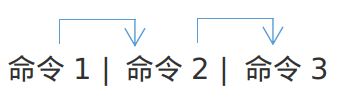
\includegraphics{shell-pipe} \caption[管道输出示意图]{管道输出示意图}\label{fig:shell-pipe}
\end{figure}

\begin{enumerate}
\def\labelenumi{\arabic{enumi}.}
\tightlist
\item
  管道命令只处理前一个命令正确输出,不处理错误输出
\item
  管道命令右边命令,必须能够接收标准输入流命令才行。
\end{enumerate}

\begin{lstlisting}[language=bash]
$ ps aux | grep "ssh"
litianci 11012  0.0  0.0  14660  1124 pts/0    S+   15:39   0:00 grep ssh
\end{lstlisting}

按一般想法,先执行了\passthrough{\lstinline!ps!},得到输出后将输出数据传递给\passthrough{\lstinline!grep!},这时候\passthrough{\lstinline!grep!}还没运行而\passthrough{\lstinline!ps!}已经运行完毕了,为什么还能统计到\passthrough{\lstinline!grep!}进程的信息呢?原因是管道实现的是进程间通信,两个进程之间存在交叉,在运行\passthrough{\lstinline!ps!}进程后开始收集进程信息,grep也已经开始并处于等待接收数据状态,当\passthrough{\lstinline!ps!}收集到任何数据后都将输出放入内存由管道传递给\passthrough{\lstinline!grep!}进行筛选。

管道其本质是数据传递,管道左边的输出数据放入内存,由管道右边的进程读取。假如内存不足以完全存放输出数据,则管道左边的进程将一直等待,直到管道右边取出内存中一部分的数据以让管道左边的进程继续输出,而管道右边的进程在管道左边的进程启动后也立刻启动了,但是它一直处于等待状态,等待接收管道传递来的数据。

也就是说,管道左右两边的进程运行几乎是没有先后顺序的。

上述管道是指匿名管道。使用匿名管道的过程中,可能已经发现管道两边的进程是同属一个进程组的,也就是说管道左方的数据只能传递给管道右方的进程,其他任何进程都没法读取此数据。但除了匿名管道,还有命名管道,命名管道是将一个进程的数据存储到一个管道文件(fifo)中,其他进程可以读取该管道文件来读取其中的数据,也就是说不再限制数据读取方。关于命名管道,请参阅Linux/Unix操作系统内核或编程类的书籍,一般都会有详细的介绍。

再来两个简单例子

\begin{lstlisting}[language=bash]
$ cat /etc/passwd | sort | less
$ gunzip < /usr/share/man/man1/grep.1.gz | nroff -c -man | less
\end{lstlisting}

\textbf{解释}

\begin{enumerate}
\def\labelenumi{\arabic{enumi}.}
\tightlist
\item
  第1行命令,\passthrough{\lstinline!cat!}
  命令显示文件\emph{/etc/passwd}的内容,输出到\passthrough{\lstinline!sort!}命令进行排序,再送给\passthrough{\lstinline!less!}命令显示出来。
\item
  第2行命令,\passthrough{\lstinline!gunzip!}
  命令解压缩\emph{grep.1.gz}文件,送给\passthrough{\lstinline!nroff!}命令调整为适合阅读的格式,传递到\passthrough{\lstinline!less!}命令显示出来。
\end{enumerate}

\hypertarget{sec:redirect}{%
\subsection{重定向}\label{sec:redirect}}

参考网页:

\begin{itemize}
\tightlist
\item
  \url{https://blog.csdn.net/u014536527/article/details/51010678}
\end{itemize}

最常见的标准输入(stdin)、标准输出(stdout)和标准错误输出(stderr)的文件描述符分别是0、1和2,其中0、1、2也可以认为是它们的数字代号。

\begin{longtable}[]{@{}cccc@{}}
\caption{三个特殊的文件}\tabularnewline
\toprule
\textbf{名称} & \textbf{程序} & \textbf{代号} &
\textbf{符号}\tabularnewline
\midrule
\endfirsthead
\toprule
\textbf{名称} & \textbf{程序} & \textbf{代号} &
\textbf{符号}\tabularnewline
\midrule
\endhead
标准输入 & /dev/stdin & 0 &
\textless{}或\textless{}\textless{}\tabularnewline
标准输出 & /dev/stdout & 1 &
\textgreater{}或\textgreater{}\textgreater{}\tabularnewline
标准错误输出 & /dev/stderr & 2 &
2\textgreater{}或2\textgreater{}\textgreater{}\tabularnewline
\bottomrule
\end{longtable}

\passthrough{\lstinline!<!}、\passthrough{\lstinline!>!}、\passthrough{\lstinline!2>!}实现的是覆盖功能,\passthrough{\lstinline!>>!}、\passthrough{\lstinline!2>>!}实现的是追加的功能,但是\passthrough{\lstinline!<<!}不是追加功能,而是表示此处生成文档(here
document),在后面cat和重定向配合的内容里有说明。此外,还有\passthrough{\lstinline!<<<!},它表示此处字符串(here
string),也见下文。

一般\passthrough{\lstinline!-!}都是表示旧工作文件夹;有时候,\passthrough{\lstinline!-!}也表示/dev/stdin,。如:

\begin{lstlisting}[language=bash]
$ cat /etc/fstab | cat -
\end{lstlisting}

脚本中常见\passthrough{\lstinline!2>\&1!}和\passthrough{\lstinline!\&>!}的符号,它们都表示将stdout和stderr都重定向到同一个地方去,即重定向所有输出内容。如最常见的\passthrough{\lstinline!\&> /dev/null!}表示将stdout或stderr丢到/dev/null表示丢弃输出信息,反过来,将/dev/null重定向到某个文件则表示清空文件。

\begin{lstlisting}[language=bash]
$ cat /dev/null > ab.sh
\end{lstlisting}

除此,还有以下几种方法快速清空文件

\begin{lstlisting}[language=bash]
$ > ab.sh
$ : > ab.sh       # 或"true >ab.sh",其实它们都等价于">ab.sh"
$ echo '' > ab.sh
$ truncate -s 0 ab.sh  # truncate命令用于收缩和扩展文件大小
$ dd if=/dev/null of=ab.sh
\end{lstlisting}

最后最重要的一点:在有重定向符号的语句中,命令执行之前已经将文件截断了。所以如果正在编辑一个文件并将编辑的结果重定向回这个文件将出现异常,因为截断后就没有合适的内容用于编辑。一个简单的示例如下:

\begin{lstlisting}[language=bash]
$ head a.log > a.log
\end{lstlisting}

有些时候直接使用\passthrough{\lstinline!>!}覆盖输出是比较危险的。可以使用\passthrough{\lstinline!set -C!}来设置如果输出重定向文件已经存在则不覆盖。使用\passthrough{\lstinline!set +C!}来取消\passthrough{\lstinline!set -C!}的效果。如果在设置了\passthrough{\lstinline!set -C!}时仍然想强制覆盖,可以使用\passthrough{\lstinline!>|!}代替\passthrough{\lstinline!>!}来重定向输出。同理错误输出也有此特性。

\begin{lstlisting}[language=bash]
$ set -C
$ cat flip >ttt.txt
-bash: ttt.txt: cannot overwrite existing file
$ cat flip >| ttt.txt
$ set +C
\end{lstlisting}

接下来讲 \passthrough{\lstinline!<<!} 一篇字符串。类似 PHP 语言的
\passthrough{\lstinline!<<<!}功能

\begin{lstlisting}[language=bash]
$ cat >log1.txt <<EOF 
> this is stdin character first!
> EOF
\end{lstlisting}

\textbf{解释}

\begin{enumerate}
\def\labelenumi{\arabic{enumi}.}
\tightlist
\item
  第1行,\passthrough{\lstinline!<<EOF!}
  表示下面另起一行,开始输入一篇字符,这篇字符直到其中一行为EOF截止。其中EOF可以换成你喜欢的字符串,一般采用大写,最好不要弄出特殊字符来。
\item
  第2行,就是输入的那篇字符。后面还可以输入很多。
\item
  第3行,输入EOF,表示这篇字符结束。
\end{enumerate}

在bash中,\passthrough{\lstinline!<<!}和\passthrough{\lstinline!<<<!}是特殊重定向符号。\passthrough{\lstinline!<<<!}
表示的是其后字符串作为输入数据。

\begin{lstlisting}[language=bash]
$ cat <<< PATH
\end{lstlisting}

等价于

\begin{lstlisting}[language=bash]
$ echo PATH | cat
\end{lstlisting}

一般情况下,重定向要么将信息输入到文件中,要么输出到屏幕上,但是既想输出到屏幕又想输出到文件就比较麻烦。使用tee的双重定向功能可以实现该想法。

\begin{lstlisting}[language=bash]
tee [-a] file
\end{lstlisting}

选项说明:

\begin{itemize}
\tightlist
\item
  -a:默认是将输出覆盖到文件中,使用该选项将变为追加行为。
\item
  file:除了输出到标准输出中,还将输出到file中。如果file为``-'',则表示再输入一次到标准输出中。
\end{itemize}

例如下面的代码,将a开头的文件内容全部保存到b.log,同时把副本交给后面的的cat,使用这个cat又将内容保存到了x.log。其中``-''代表前面的stdin。

\begin{lstlisting}[language=bash]
$ cat a* | tee b.log | cat - >x.log
\end{lstlisting}

还可以直接输出到屏幕:

\begin{lstlisting}[language=bash]
$ cat a* | tee b.log | cat
\end{lstlisting}

tee默认会使用覆盖的方式保存到文件,可以使用-a选项来追加到文件。如:

\begin{lstlisting}[language=bash]
$ cat a* | tee -a b.log | cat
\end{lstlisting}

\subsection{重定向和管道的区别}

\begin{longtable}[]{@{}ll@{}}
\caption{管道命令与重定向区别}\tabularnewline
\toprule
\begin{minipage}[b]{0.55\columnwidth}\raggedright
\textbf{管道(\passthrough{\lstinline!|!})}\strut
\end{minipage} & \begin{minipage}[b]{0.40\columnwidth}\raggedright
\textbf{重定向(\passthrough{\lstinline!>!},\passthrough{\lstinline!<!})}\strut
\end{minipage}\tabularnewline
\midrule
\endfirsthead
\toprule
\begin{minipage}[b]{0.55\columnwidth}\raggedright
\textbf{管道(\passthrough{\lstinline!|!})}\strut
\end{minipage} & \begin{minipage}[b]{0.40\columnwidth}\raggedright
\textbf{重定向(\passthrough{\lstinline!>!},\passthrough{\lstinline!<!})}\strut
\end{minipage}\tabularnewline
\midrule
\endhead
\begin{minipage}[t]{0.55\columnwidth}\raggedright
左边命令应该做到标准输出,右边命令应该接受标准输入\strut
\end{minipage} & \begin{minipage}[t]{0.40\columnwidth}\raggedright
左边的命令应该有标准输出(输入),右边只能是文件\strut
\end{minipage}\tabularnewline
\begin{minipage}[t]{0.55\columnwidth}\raggedright
管道触发两个子进程执行\passthrough{\lstinline!|!}两边的程序\strut
\end{minipage} & \begin{minipage}[t]{0.40\columnwidth}\raggedright
在一个进程内执行\strut
\end{minipage}\tabularnewline
\bottomrule
\end{longtable}

\begin{lstlisting}[language=bash]
$ cat test.sh| grep -n 'echo' #“|”管道两边都必须是shell命令
$ grep -n 'echo' <test.sh #“重定向”符号,右边只能是文件
\end{lstlisting}

下面两个也是等同的。

\begin{lstlisting}[language=bash]
$ (sed -n '1,$p'|grep -n 'echo')<test.sh 
\end{lstlisting}

这个脚本比较有意思了。由于前面是管道,后面需要把test.sh内容重定向到 sed
,然后sed输出通过管道,输入给grep.需要将前面用``()''运算符括起来。在单括号内的命令,可以把它们看作一个象一个命令样。如果不加括号test.sh就是grep
的输入了。

\begin{lstlisting}[language=bash]
$ sed -n '1,$p'<test.sh | grep -n 'echo'
\end{lstlisting}

重定向运算符,在shell命令解析前,首先检查的(一个命令,执行前一定检查好它的输入,输出,也就是0,1,2
设备是否准备好),所以优先级会最高

\begin{lstlisting}[language=bash]
$ sed -n '1,10p'<test.sh | grep -n 'echo' <testsh.sh
\end{lstlisting}

哈哈,这个grep又接受管道输入,又有testsh.sh输入,那是不是2个都接收呢。刚才说了``\textless{}''运算符会优先,管道还没有发送数据前,grep绑定了testsh.sh输入,这样sed命令输出就被抛弃了。这里一定要小心使用

下面是输出重定向例子。

\begin{lstlisting}[language=bash]
$ cat test.sh>test.txt
$ cat test.sh|tee test.txt &>/dev/null
\end{lstlisting}

通过管道实现将结果存入文件,还需要借助命令tee,它会把管道过来标准输入写入文件test.txt
,然后将标准输入复制到标准输出(stdout),所以重定向到/dev/null
不显示输出。``\textgreater{}''输出重定向,往往在命令最右边,接收左边命令的,输出结果,重定向到指定文件。也可以用到命令中间。

\begin{lstlisting}[language=bash]
$ ls test.sh test1.sh testsh.sh 2>err.txt | grep 'test'
\end{lstlisting}

目录下面有:test,testsh文件,test1.sh不存在,因此将ls
命令错误输出输入到err.txt 正确输出,还会通过管道发送到grep命令。

\begin{lstlisting}[language=bash]
$ ls test.sh test1.sh testsh.sh &>err.txt | grep 'test'
\end{lstlisting}

这次打印结果是空,\&代表正确与错误输出
都输入给err.txt,通过管道继续往下面传递数据为空,所以没有什么显示的。
同样``\textgreater{}''输出重定向符,优先级也是先解析,当一个命令有这个字符,它就会与左边命令标准输出绑定。准备好了这些,就等待命令执行输出数据,它就开始接收

从上面例子可以看,重定向与管道在使用时候很多时候可以通用,其实,在shell里面,经常是【条条大路通罗马】的。一般如果是命令间传递参数,还是管道的好,如果处理输出结果需要重定向到文件,还是用重定向输出比较好。

\subsection{顺序执行}

顺序执行,类似C语言的\passthrough{\lstinline!;!}语法。逐条执行命令。

\begin{lstlisting}[language=bash]
$ date ; cat <<< LONGLONGJOB | cat - ; date
2018年 09月 29日 星期六 17:16:12 CST
LONGLONGJOB
2018年 09月 29日 星期六 17:16:12 CST
\end{lstlisting}

\textbf{解释}

\begin{enumerate}
\def\labelenumi{\arabic{enumi}.}
\tightlist
\item
  本命令实现了对程序耗时的计算。而分号\passthrough{\lstinline!;!}的优先级是低于管道的。最终送给\passthrough{\lstinline!cat -!}中\passthrough{\lstinline!cat!}的只有\passthrough{\lstinline!LONGLONGJOB!}。
\end{enumerate}

\subsection{后台命令}

有些命令比较耗时,或者其他原因,我们希望他们运行在后台。就可以用如下方式。

\begin{lstlisting}[language=bash]
$ tar cf test.tar test &
[1] 9355
$ 
[1]+  已完成               tar cf test.tar test
\end{lstlisting}

\textbf{解释}

\begin{enumerate}
\def\labelenumi{\arabic{enumi}.}
\tightlist
\item
  第1行,命令末尾加\passthrough{\lstinline!\&!}即可让程序运行于后台。shell
  会告诉该命令的进程号,示例中为\passthrough{\lstinline!9355!};并且会为他编号。
\item
  第4行,命令运行介绍,shell 会告诉你已经完成了该后台命令。
\item
  在运行过程中,如果你不想让他终止,请不要关闭该 shell。
\end{enumerate}

\subsection{命令扩展}

把命令输出结果作为另外一条命令的参数,也是常用的一项功能,可以用美元符号\passthrough{\lstinline!$!}和斜点(键盘左上角~键)\passthrough{\lstinline!`!},\passthrough{\lstinline!$(command)!}
和 \passthrough{\lstinline!`command`!}。

\begin{lstlisting}[language=bash]
$ vim -p $(find ~ | grep deepin-bible.tex)
\end{lstlisting}

\textbf{解释}

\begin{enumerate}
\def\labelenumi{\arabic{enumi}.}
\tightlist
\item
  \passthrough{\lstinline!find \~!}查找主目录所有文件,\passthrough{\lstinline!grep deepin-bible.tex!}
  从前者找到文件名包含\passthrough{\lstinline!deepin-bible.tex!}的所有文件,vim
  把找到的所有文件打开。
\end{enumerate}

\subsection{简单数值计算}

使用\passthrough{\lstinline!$[math expression]!}的方式计算。

\begin{lstlisting}[language=bash]
$ echo "我今年$[`date +%Y` - 1987]岁了。"
我今年31岁了。
\end{lstlisting}

\textbf{解释}

\begin{enumerate}
\def\labelenumi{\arabic{enumi}.}
\tightlist
\item
  \passthrough{\lstinline!`date +\%Y`!}输出今年年数2018,\passthrough{\lstinline!$[2018 - 1987]!}输出岁数。
\end{enumerate}

\subsection{输出变量值}

一些变量的数值,可以通过\passthrough{\lstinline!$Var!}输出。

\begin{lstlisting}[language=bash]
$ echo $PATH
\end{lstlisting}

\hypertarget{shell-variables}{%
\section{Shell 变量(Variables)}\label{shell-variables}}

参考网页:

\begin{itemize}
\tightlist
\item
  \url{https://blog.csdn.net/apollon_krj/article/details/70148022}
\end{itemize}

变量分为全局变量(环境变量)和局部变量(本地变量)
。环境变量可以在定义它们的shell及其派生出来的任意子进程的shell中使用。局部变量只能在定义它们的函数/脚本中使用。还有一些变量是用户创建的,其他的则是专用的shell变量,比如系统变量\passthrough{\lstinline!$0!}等。

\textbf{全局变量(环境变量)}

环境变量可用于定义shell的运行环境,环境变量可以在配置文件中定义与修改,也可以在命令行中设置,但是命令行中的修改操作在终端重启时就会丢失,因此最好在配置文件中修改(用户家目录的``.bash\_profile``文件或者全局配置``/etc/profile''、``/etc/bashrc''文件或者``/etc/profile.d''文件中定义。)将环境变量放在profile文件中,每次用户登录时这些变量值将被初始化。比如HOME、USER、SHELL、UID等再用户登录之前就已经被/bin/login程序设置好了。

摘自《Linux Bible》

\begin{longtable}[]{@{}cl@{}}
\caption{常见环境变量表}\tabularnewline
\toprule
\begin{minipage}[b]{0.23\columnwidth}\centering
\textbf{变量}\strut
\end{minipage} & \begin{minipage}[b]{0.72\columnwidth}\raggedright
\textbf{解释}\strut
\end{minipage}\tabularnewline
\midrule
\endfirsthead
\toprule
\begin{minipage}[b]{0.23\columnwidth}\centering
\textbf{变量}\strut
\end{minipage} & \begin{minipage}[b]{0.72\columnwidth}\raggedright
\textbf{解释}\strut
\end{minipage}\tabularnewline
\midrule
\endhead
\begin{minipage}[t]{0.23\columnwidth}\centering
\passthrough{\lstinline!BASH!}\strut
\end{minipage} & \begin{minipage}[t]{0.72\columnwidth}\raggedright
bash 命令的全路径地址,通常为 \emph{/bin/bash}。\strut
\end{minipage}\tabularnewline
\begin{minipage}[t]{0.23\columnwidth}\centering
\passthrough{\lstinline!BASH\_VERSION!}\strut
\end{minipage} & \begin{minipage}[t]{0.72\columnwidth}\raggedright
bash 版本号。\strut
\end{minipage}\tabularnewline
\begin{minipage}[t]{0.23\columnwidth}\centering
\passthrough{\lstinline!EUID!}\strut
\end{minipage} & \begin{minipage}[t]{0.72\columnwidth}\raggedright
这是当前用户的有效用户ID号,Shell启动时分配,基于用户在
\emph{/etc/passwd} 的分配。\strut
\end{minipage}\tabularnewline
\begin{minipage}[t]{0.23\columnwidth}\centering
\passthrough{\lstinline!FCEDIT!}\strut
\end{minipage} & \begin{minipage}[t]{0.72\columnwidth}\raggedright
如果设置该变量,表示使用\passthrough{\lstinline!fc!}命令来编辑命令记录(history
commands);否则改用\passthrough{\lstinline!vi!}命令。\strut
\end{minipage}\tabularnewline
\begin{minipage}[t]{0.23\columnwidth}\centering
\passthrough{\lstinline!HISTFILE!}\strut
\end{minipage} & \begin{minipage}[t]{0.72\columnwidth}\raggedright
命令记录文件,通常为 \emph{\$HOME/.bash\_history}。\strut
\end{minipage}\tabularnewline
\begin{minipage}[t]{0.23\columnwidth}\centering
\passthrough{\lstinline!HISTFILESIZE!}\strut
\end{minipage} & \begin{minipage}[t]{0.72\columnwidth}\raggedright
命令记录条数,当超过此数,循环记录,最久的记录被删除。默认值1000。\strut
\end{minipage}\tabularnewline
\begin{minipage}[t]{0.23\columnwidth}\centering
\passthrough{\lstinline!HISTCMD!}\strut
\end{minipage} & \begin{minipage}[t]{0.72\columnwidth}\raggedright
返回当前命令处于命令记录的序号。\strut
\end{minipage}\tabularnewline
\begin{minipage}[t]{0.23\columnwidth}\centering
\passthrough{\lstinline!HOME!}\strut
\end{minipage} & \begin{minipage}[t]{0.72\columnwidth}\raggedright
当前用户的主目录,也就是你登录后,或者输入\passthrough{\lstinline!cd!}回车跳到的文件夹。常用符号\passthrough{\lstinline!~!}表示主目录。\strut
\end{minipage}\tabularnewline
\begin{minipage}[t]{0.23\columnwidth}\centering
\passthrough{\lstinline!HOSTTYPE!}\strut
\end{minipage} & \begin{minipage}[t]{0.72\columnwidth}\raggedright
当前计算机硬件体系,比如 Intel 兼容机,一般是 i386, i486, i586, i686,
或者 i386 等数值。对于AMD 64位机,一般是 x86\_64。\strut
\end{minipage}\tabularnewline
\begin{minipage}[t]{0.23\columnwidth}\centering
\passthrough{\lstinline!MAIL!}\strut
\end{minipage} & \begin{minipage}[t]{0.72\columnwidth}\raggedright
邮箱文件。深度普通用户一般都没有设置该变量,root用户一般为\emph{/var/mail/root}。对于centos
系列一般为 \emph{/var/spool/mail/}\strut
\end{minipage}\tabularnewline
\begin{minipage}[t]{0.23\columnwidth}\centering
\passthrough{\lstinline!OLDPWD!}\strut
\end{minipage} & \begin{minipage}[t]{0.72\columnwidth}\raggedright
前一个工作目录。当你频繁在两个目录切换的时候,当前目录的前一个目录就存储在该变量。通常使用减号\passthrough{\lstinline!-!}表示。使用\passthrough{\lstinline!cd -!}
可以跳转到前一个目录。\strut
\end{minipage}\tabularnewline
\begin{minipage}[t]{0.23\columnwidth}\centering
\passthrough{\lstinline!OSTYPE!}\strut
\end{minipage} & \begin{minipage}[t]{0.72\columnwidth}\raggedright
本机操作系统类型。比如\passthrough{\lstinline!linux!}或\passthrough{\lstinline!linux-gnu!}\strut
\end{minipage}\tabularnewline
\begin{minipage}[t]{0.23\columnwidth}\centering
\passthrough{\lstinline!PATH!}\strut
\end{minipage} & \begin{minipage}[t]{0.72\columnwidth}\raggedright
路径变量。一般为一长串字符,用英文冒号\passthrough{\lstinline!:!}拼接多个文件夹。Windows
系统也有该变量,只不过使用英文分号\passthrough{\lstinline!;!}拼接的。处于上述文件夹下的可执行文件,只需输入本文件名不用输入完整路径,即可被shell找到执行。shell是从前往后找的,重名可执行文件,需要注意执行的是不是自己的文件。不在\passthrough{\lstinline!PATH!}目录集合下的可执行文件,则需要输入绝对路径或者相对路径才可以执行。例如本机的root用户,\passthrough{\lstinline!PATH=/usr/local/sbin:/usr/local/bin:/usr/sbin:/usr/bin:/sbin:/bin!}。\strut
\end{minipage}\tabularnewline
\begin{minipage}[t]{0.23\columnwidth}\centering
\passthrough{\lstinline!PPID!}\strut
\end{minipage} & \begin{minipage}[t]{0.72\columnwidth}\raggedright
当前shell父进程ID号。\strut
\end{minipage}\tabularnewline
\begin{minipage}[t]{0.23\columnwidth}\centering
\passthrough{\lstinline!PROMPT\_COMMAND!}\strut
\end{minipage} & \begin{minipage}[t]{0.72\columnwidth}\raggedright
深度操作系统没有设置该变量。通常该变量为一条命令名称。在命令提示符(shell
prompt)每次出现之前执行。\strut
\end{minipage}\tabularnewline
\begin{minipage}[t]{0.23\columnwidth}\centering
\passthrough{\lstinline!PS1!}\strut
\end{minipage} & \begin{minipage}[t]{0.72\columnwidth}\raggedright
设置命令提示符。有时还会有\passthrough{\lstinline!PS2!},
\passthrough{\lstinline!PS3!}等。\strut
\end{minipage}\tabularnewline
\begin{minipage}[t]{0.23\columnwidth}\centering
\passthrough{\lstinline!PWD!}\strut
\end{minipage} & \begin{minipage}[t]{0.72\columnwidth}\raggedright
当前工作目录。\strut
\end{minipage}\tabularnewline
\begin{minipage}[t]{0.23\columnwidth}\centering
\passthrough{\lstinline!RANDOM!}\strut
\end{minipage} & \begin{minipage}[t]{0.72\columnwidth}\raggedright
返回 0 到 99999 的一个随机数。\strut
\end{minipage}\tabularnewline
\begin{minipage}[t]{0.23\columnwidth}\centering
\passthrough{\lstinline!SECONDS!}\strut
\end{minipage} & \begin{minipage}[t]{0.72\columnwidth}\raggedright
返回当前shell启用了多少秒数。\strut
\end{minipage}\tabularnewline
\begin{minipage}[t]{0.23\columnwidth}\centering
\passthrough{\lstinline!SHLVL!}\strut
\end{minipage} & \begin{minipage}[t]{0.72\columnwidth}\raggedright
这是与当前shell会话相关联的shell级别的数目。当您登录到shell时,\passthrough{\lstinline!SHLVL!}为1。每次你新开
bash,比如使用\passthrough{\lstinline!su!}或者键入\passthrough{\lstinline!bash!},该数字都会加一。\strut
\end{minipage}\tabularnewline
\begin{minipage}[t]{0.23\columnwidth}\centering
\passthrough{\lstinline!TMOUT!}\strut
\end{minipage} & \begin{minipage}[t]{0.72\columnwidth}\raggedright
深度操作系统没有设置该变量。设置一定秒数,如果 shell
在设定时间内没有输入,则退出。对于服务器来说,还是跟安全很相关的一个变量。\strut
\end{minipage}\tabularnewline
\bottomrule
\end{longtable}

可以用\passthrough{\lstinline!echo!}来显示查看全局变量(eg:\passthrough{\lstinline!echo $HOME!})。\passthrough{\lstinline!env!}(或\passthrough{\lstinline!printenv!})、\passthrough{\lstinline!set!}也可以用来查看系统的环境变量,但不是单独查看。而用\passthrough{\lstinline!unset!}临时取消环境变量(eg:\passthrough{\lstinline!unset USER!}),要永久生效还是要写到配置文件中

自定义环境变量(采用export):

\begin{itemize}
\tightlist
\item
  export 变量名=value
\item
  变量名=value;export 变量名
\item
  declare -x 变量名=value
\end{itemize}

这里依旧是临时生效,在shell终端关闭后就消失了,写到配置文件中则永久生效(注意:写到配置文件中后需要运行一遍配置文件的脚本才可生效,否则等重启时生效)

命令行的三种方式测试如下:

关于环境变量PATH与export的更详细的内容,可参考:
Linux环境变量与系统编程学习笔记

2、局部变量(本地变量):

本地变量在用户当前的shell生存期的脚本中使用。在一个函数中将某个变量声明为local,则该变量就是一个局部变量,只在本函数中有效。
定义:

\begin{itemize}
\tightlist
\item
  变量名=value
\item
  变量名='value'
\item
  变量名=''value''
\end{itemize}

shell中变量名的要求:一般遵循字母、数字、下滑线组成,不能以数字开头

\subsection{别名的创建和使用}

为了方便,常会配置一些别名。

\begin{lstlisting}[language=bash]
$ alias l='ls -CF'
$ alias la='ls -A'
$ alias rm='rm -i
$ alias
$ \ls
$ unalias la
$ alias
\end{lstlisting}

\textbf{解释}

\begin{enumerate}
\def\labelenumi{\arabic{enumi}.}
\tightlist
\item
  第1-3行,定义了三个别名。这些别名相当于后面的那个命令。
\item
  第4行,查看当前所有别名。
\item
  第5行,使用\passthrough{\lstinline!\\command!}表示,使用最原始的命令,非别名。
\item
  第6-7行,暂时取消别名\passthrough{\lstinline!la!},然后查看当前所有的别名。这个\passthrough{\lstinline!unalias!}只可以在当前shell取消别名。
\end{enumerate}

\hypertarget{-shell}{%
\subsection{退出 shell}\label{-shell}}

可以使用快捷键\passthrough{\lstinline!Ctrl+D!},或者输入\passthrough{\lstinline!exit!},或者直接点击窗口的关闭按钮。

\hypertarget{-shell-}{%
\section{定制 shell 环境}\label{-shell-}}

bash 的配置文件,一般如下表所示,

\begin{longtable}[]{@{}cl@{}}
\caption{Bash 配置文件说明}\tabularnewline
\toprule
\begin{minipage}[b]{0.20\columnwidth}\centering
\textbf{文件}\strut
\end{minipage} & \begin{minipage}[b]{0.74\columnwidth}\raggedright
\textbf{解释}\strut
\end{minipage}\tabularnewline
\midrule
\endfirsthead
\toprule
\begin{minipage}[b]{0.20\columnwidth}\centering
\textbf{文件}\strut
\end{minipage} & \begin{minipage}[b]{0.74\columnwidth}\raggedright
\textbf{解释}\strut
\end{minipage}\tabularnewline
\midrule
\endhead
\begin{minipage}[t]{0.20\columnwidth}\centering
/etc/profile\strut
\end{minipage} & \begin{minipage}[t]{0.74\columnwidth}\raggedright
影响所有用户,首次登录时执行。通常在此配置\passthrough{\lstinline!PATH!},\passthrough{\lstinline!MAIL!},\passthrough{\lstinline!HISTFILESIZE!}等。最后,该文件会读取\emph{/etc/profile.d}
文件夹下其他 shell 配置文件。\strut
\end{minipage}\tabularnewline
\begin{minipage}[t]{0.20\columnwidth}\centering
/etc/bashrc\strut
\end{minipage} & \begin{minipage}[t]{0.74\columnwidth}\raggedright
影响所有 bash 用户,每次打开 bash 都会执行。通常在此配置提示(prompt)
\passthrough{\lstinline!PS1!}和一些别名。变量设置会被用户自己的
\emph{\passthrough{\lstinline!~!}/.bashrc}覆盖。\strut
\end{minipage}\tabularnewline
\begin{minipage}[t]{0.20\columnwidth}\centering
\textasciitilde{}/.bash\_profile\strut
\end{minipage} & \begin{minipage}[t]{0.74\columnwidth}\raggedright
只影响该用户,首次登录时执行。一般存放环境变量,并会调用\emph{\passthrough{\lstinline!~!}/.bashrc}文件,特别适合放置环境变量。\strut
\end{minipage}\tabularnewline
\begin{minipage}[t]{0.20\columnwidth}\centering
\textasciitilde{}/.bashrc\strut
\end{minipage} & \begin{minipage}[t]{0.74\columnwidth}\raggedright
只影响该用户,每次打开 bash
都会执行。存放一些自己的配置,特别适合放置别名。\strut
\end{minipage}\tabularnewline
\begin{minipage}[t]{0.20\columnwidth}\centering
\textasciitilde{}/.bash\_logout\strut
\end{minipage} & \begin{minipage}[t]{0.74\columnwidth}\raggedright
只影响该用户,每次注销(退出最后一个shell时)执行。通常只有清屏功能。\strut
\end{minipage}\tabularnewline
\bottomrule
\end{longtable}

一般,修改\emph{/etc/profile},\emph{/etc/bashrc}需要root权限,而且影响所有用户。后面三个文件,只影响本用户。

编辑好这些文件,需要执行才可以生效。

\begin{lstlisting}[language=bash]
$ gedit $HOME/.bashrc #编辑文件
$ source $HOME/.bashrc #执行生效
\end{lstlisting}

\hypertarget{prompt}{%
\subsection{配置提示(prompt)}\label{prompt}}

参考网页:

\begin{itemize}
\tightlist
\item
  \url{https://www.cnblogs.com/lienhua34/p/5018119.html}
\item
  \url{http://billie66.github.io/TLCL/book/chap14.html}
\end{itemize}

Linux系统终端提示符,就是在前面\ref{shell:intro}提到的\passthrough{\lstinline!$!}或者\passthrough{\lstinline!#!}之前的文字。是通过环境变量\passthrough{\lstinline!PS1!},\passthrough{\lstinline!PS2!},\passthrough{\lstinline!PS3!},\passthrough{\lstinline!PS4!}配置的。一般都是配置系统环境变量\passthrough{\lstinline!PS1!}(是\cqh prompt
string
one\cqt 的简写)定义。通过命令\passthrough{\lstinline!echo $PS1!}查看当前设置。

\begin{lstlisting}[language=bash]
$ echo $PS1
\[\e]0;\u@\h: \w\a\]${debian_chroot:+($debian_chroot)}\[\033[01;32m\]\u@\h\[\033[00m\]:\[\033[01;34m\]\w\[\033[00m\]$\setminus\$$
\end{lstlisting}

\textbf{1、基本转义字符}

PS1的值由一系列静态文本或\passthrough{\lstinline!\\!}和转义字符序列组成。示例,

\begin{lstlisting}[language=bash]
$ PS1="\u@\H \w$ "
\end{lstlisting}

\begin{longtable}[]{@{}ll@{}}
\caption{Shell 提示符中用到的转义字符}\tabularnewline
\toprule
\begin{minipage}[b]{0.22\columnwidth}\raggedright
\textbf{序列}\strut
\end{minipage} & \begin{minipage}[b]{0.72\columnwidth}\raggedright
\textbf{显示值}\strut
\end{minipage}\tabularnewline
\midrule
\endfirsthead
\toprule
\begin{minipage}[b]{0.22\columnwidth}\raggedright
\textbf{序列}\strut
\end{minipage} & \begin{minipage}[b]{0.72\columnwidth}\raggedright
\textbf{显示值}\strut
\end{minipage}\tabularnewline
\midrule
\endhead
\begin{minipage}[t]{0.22\columnwidth}\raggedright
\passthrough{\lstinline!\\a!}\strut
\end{minipage} & \begin{minipage}[t]{0.72\columnwidth}\raggedright
以 ASCII
格式编码的铃声。当遇到这个转义序列时,计算机会发出嗡嗡的响声。\strut
\end{minipage}\tabularnewline
\begin{minipage}[t]{0.22\columnwidth}\raggedright
\passthrough{\lstinline!\\d!}\strut
\end{minipage} & \begin{minipage}[t]{0.72\columnwidth}\raggedright
以日,月,天格式来表示当前日期。例如,``Mon May 26''\strut
\end{minipage}\tabularnewline
\begin{minipage}[t]{0.22\columnwidth}\raggedright
\passthrough{\lstinline!\\h!}\strut
\end{minipage} & \begin{minipage}[t]{0.72\columnwidth}\raggedright
本地机的主机名,但不带末尾的域名。\strut
\end{minipage}\tabularnewline
\begin{minipage}[t]{0.22\columnwidth}\raggedright
\passthrough{\lstinline!\\H!}\strut
\end{minipage} & \begin{minipage}[t]{0.72\columnwidth}\raggedright
完整的主机名。\strut
\end{minipage}\tabularnewline
\begin{minipage}[t]{0.22\columnwidth}\raggedright
\passthrough{\lstinline!\\j!}\strut
\end{minipage} & \begin{minipage}[t]{0.72\columnwidth}\raggedright
运行在当前 shell 会话中的工作数。\strut
\end{minipage}\tabularnewline
\begin{minipage}[t]{0.22\columnwidth}\raggedright
\passthrough{\lstinline!\\l!}\strut
\end{minipage} & \begin{minipage}[t]{0.72\columnwidth}\raggedright
当前终端设备名。\strut
\end{minipage}\tabularnewline
\begin{minipage}[t]{0.22\columnwidth}\raggedright
\passthrough{\lstinline!\\n!}\strut
\end{minipage} & \begin{minipage}[t]{0.72\columnwidth}\raggedright
一个换行符。\strut
\end{minipage}\tabularnewline
\begin{minipage}[t]{0.22\columnwidth}\raggedright
\passthrough{\lstinline!\\r!}\strut
\end{minipage} & \begin{minipage}[t]{0.72\columnwidth}\raggedright
一个回车符。\strut
\end{minipage}\tabularnewline
\begin{minipage}[t]{0.22\columnwidth}\raggedright
\passthrough{\lstinline!\\s!}\strut
\end{minipage} & \begin{minipage}[t]{0.72\columnwidth}\raggedright
shell 程序名。\strut
\end{minipage}\tabularnewline
\begin{minipage}[t]{0.22\columnwidth}\raggedright
\passthrough{\lstinline!\\t!}\strut
\end{minipage} & \begin{minipage}[t]{0.72\columnwidth}\raggedright
以24小时制,hours:minutes:seconds 的格式表示当前时间。\strut
\end{minipage}\tabularnewline
\begin{minipage}[t]{0.22\columnwidth}\raggedright
\passthrough{\lstinline!\\T!}\strut
\end{minipage} & \begin{minipage}[t]{0.72\columnwidth}\raggedright
以12小时制表示当前时间。\strut
\end{minipage}\tabularnewline
\begin{minipage}[t]{0.22\columnwidth}\raggedright
\passthrough{\lstinline!\\@!}\strut
\end{minipage} & \begin{minipage}[t]{0.72\columnwidth}\raggedright
以12小时制,AM/PM 格式来表示当前时间,例如``10:51 PM''。\strut
\end{minipage}\tabularnewline
\begin{minipage}[t]{0.22\columnwidth}\raggedright
\passthrough{\lstinline!\\A!}\strut
\end{minipage} & \begin{minipage}[t]{0.72\columnwidth}\raggedright
以24小时制,hours:minutes 格式表示当前时间。\strut
\end{minipage}\tabularnewline
\begin{minipage}[t]{0.22\columnwidth}\raggedright
\passthrough{\lstinline!\\u!}\strut
\end{minipage} & \begin{minipage}[t]{0.72\columnwidth}\raggedright
当前用户名。\strut
\end{minipage}\tabularnewline
\begin{minipage}[t]{0.22\columnwidth}\raggedright
\passthrough{\lstinline!\\v!}\strut
\end{minipage} & \begin{minipage}[t]{0.72\columnwidth}\raggedright
shell 程序的版本号,例如4.3。\strut
\end{minipage}\tabularnewline
\begin{minipage}[t]{0.22\columnwidth}\raggedright
\passthrough{\lstinline!\\V!}\strut
\end{minipage} & \begin{minipage}[t]{0.72\columnwidth}\raggedright
shell 程序的版本号,例如4.3.11。\strut
\end{minipage}\tabularnewline
\begin{minipage}[t]{0.22\columnwidth}\raggedright
\passthrough{\lstinline!\\w!}\strut
\end{minipage} & \begin{minipage}[t]{0.72\columnwidth}\raggedright
当前工作目录名。\strut
\end{minipage}\tabularnewline
\begin{minipage}[t]{0.22\columnwidth}\raggedright
\passthrough{\lstinline!\\W!}\strut
\end{minipage} & \begin{minipage}[t]{0.72\columnwidth}\raggedright
当前工作目录名的最后部分。\strut
\end{minipage}\tabularnewline
\begin{minipage}[t]{0.22\columnwidth}\raggedright
\passthrough{\lstinline"\\!"}\strut
\end{minipage} & \begin{minipage}[t]{0.72\columnwidth}\raggedright
当前命令的历史号。\strut
\end{minipage}\tabularnewline
\begin{minipage}[t]{0.22\columnwidth}\raggedright
\passthrough{\lstinline!\\#!}\strut
\end{minipage} & \begin{minipage}[t]{0.72\columnwidth}\raggedright
当前 shell 会话中的命令数。\strut
\end{minipage}\tabularnewline
\begin{minipage}[t]{0.22\columnwidth}\raggedright
\passthrough{\lstinline!\\$!}\strut
\end{minipage} & \begin{minipage}[t]{0.72\columnwidth}\raggedright
这会显示一个\passthrough{\lstinline!$!}字符,除非你拥有超级用户权限。在那种情况下,
它会显示一个\passthrough{\lstinline!#!}字符。\strut
\end{minipage}\tabularnewline
\begin{minipage}[t]{0.22\columnwidth}\raggedright
\passthrough{\lstinline!\\[!}\strut
\end{minipage} & \begin{minipage}[t]{0.72\columnwidth}\raggedright
标志着一系列一个或多个非打印字符的开始。这被用来嵌入非打印的控制字符,这些字符以某种方式来操作终端仿真器,比方说移动光标或者是更改文本颜色。\strut
\end{minipage}\tabularnewline
\begin{minipage}[t]{0.22\columnwidth}\raggedright
\passthrough{\lstinline!\\]!}\strut
\end{minipage} & \begin{minipage}[t]{0.72\columnwidth}\raggedright
标志着非打印字符序列结束。\strut
\end{minipage}\tabularnewline
\bottomrule
\end{longtable}

\textbf{2、字体颜色}

上面能够满足我们的效果了,但是相对于LinuxMint原始的提示符,缺少了颜色,不太美观。下面我们来学习如何添加颜色。大多数终端仿真器程序支持一定的非打印字符序列来控制,比方说字符属性(像颜色,黑体和可怕的闪烁)
和光标位置。

字体颜色是由一个ANSI
转义编码来控制的。该控制编码会嵌入字符流中并发送给终端仿真器。但是,该控制编码不会被``打印''到屏幕上,而是会被终端解释为一个指令。正如我们在上表看到的字符序列,这个\passthrough{\lstinline!\\[!}和\passthrough{\lstinline!\\]!}序列被用来封装这些非打印字符。一个
ANSI
转义编码以一个八进制033(这个编码是由退出按键产生的)开头,其后跟着一个可选的字符属性(0:正常、1:黑体、4:下划线、5:闪烁、7:反向(前景色和背景色反转)),在之后是一个指令。

\begin{longtable}[]{@{}cccc@{}}
\caption{用转义序列来设置文本颜色}\tabularnewline
\toprule
\textbf{序列} & \textbf{文本颜色} & \textbf{序列} &
\textbf{文本颜色}\tabularnewline
\midrule
\endfirsthead
\toprule
\textbf{序列} & \textbf{文本颜色} & \textbf{序列} &
\textbf{文本颜色}\tabularnewline
\midrule
\endhead
\textbackslash{}033{[}0;30m & 黑色 & \textbackslash{}033{[}1;30m &
深灰色\tabularnewline
\textbackslash{}033{[}0;31m & 红色 & \textbackslash{}033{[}1;31m &
浅红色\tabularnewline
\textbackslash{}033{[}0;32m & 绿色 & \textbackslash{}033{[}1;32m &
浅绿色\tabularnewline
\textbackslash{}033{[}0;33m & 棕色 & \textbackslash{}033{[}1;33m &
黄色\tabularnewline
\textbackslash{}033{[}0;34m & 蓝色 & \textbackslash{}033{[}1;34m &
浅蓝色\tabularnewline
\textbackslash{}033{[}0;35m & 粉红 & \textbackslash{}033{[}1;35m &
浅粉色\tabularnewline
\textbackslash{}033{[}0;36m & 青色 & \textbackslash{}033{[}1;36m &
浅青色\tabularnewline
\textbackslash{}033{[}0;37m & 浅灰色 & \textbackslash{}033{[}1;37m &
白色\tabularnewline
\bottomrule
\end{longtable}

例如我们来设置一个同LinuxMint默认的绿色提示符,

\begin{lstlisting}[language=bash]
$ PS1="\[\033[01;32m\]\u@\W$\setminus\$$\[\033[00m\] "
\end{lstlisting}

于是,我们便有了下面的效果。

上面跟设置的提示符格式中的最后那个\passthrough{\lstinline!”\\[\\033[00m\\]”!}是用于将后续的字符颜色还原回原来的颜色。如果没有没有加最后这个转义码,则会出现下面结果(我们自己手工输入的命令也都将是绿色的)。

\textbf{3、背景颜色}

除了字体颜色,我们也可以设置字体的背景颜色。同样是通过转义的控制编码来实现,下表是背景颜色的控制编码。

\begin{longtable}[]{@{}cccc@{}}
\caption{用转义序列来设置背景颜色}\tabularnewline
\toprule
\textbf{序列} & \textbf{文本颜色} & \textbf{序列} &
\textbf{文本颜色}\tabularnewline
\midrule
\endfirsthead
\toprule
\textbf{序列} & \textbf{文本颜色} & \textbf{序列} &
\textbf{文本颜色}\tabularnewline
\midrule
\endhead
\textbackslash{}033{[}0;40m & 黑色 & \textbackslash{}033{[}1;44m &
蓝色\tabularnewline
\textbackslash{}033{[}0;41m & 红色 & \textbackslash{}033{[}1;45m &
粉红\tabularnewline
\textbackslash{}033{[}0;42m & 绿色 & \textbackslash{}033{[}1;46m &
青色\tabularnewline
\textbackslash{}033{[}0;43m & 棕色 & \textbackslash{}033{[}1;47m &
浅灰色\tabularnewline
\bottomrule
\end{longtable}

\textbf{4、移动光标}

转义编码也可以用来定位光标。这些编码通常被用来,每次当提示符出现的时候,会在屏幕的不同位置,比如说上面一个角落,显示一个时钟或者其它一些信息。下表是一系列用来定位光标的转义编码:

\begin{longtable}[]{@{}cl@{}}
\caption{光标移动转义序列}\tabularnewline
\toprule
\textbf{转义编码} & \textbf{行动}\tabularnewline
\midrule
\endfirsthead
\toprule
\textbf{转义编码} & \textbf{行动}\tabularnewline
\midrule
\endhead
\textbackslash{}033{[}l;cH & 把光标移到第 l 行,第 c 列。\tabularnewline
\textbackslash{}033{[}nA & 把光标向上移动 n 行。\tabularnewline
\textbackslash{}033{[}nB & 把光标向下移动 n 行。\tabularnewline
\textbackslash{}033{[}nC & 把光标向前移动 n 个字符。\tabularnewline
\textbackslash{}033{[}nD & 把光标向后移动 n 个字符。\tabularnewline
\textbackslash{}033{[}2J &
清空屏幕,把光标移到左上角(第零行,第零列)。\tabularnewline
\textbackslash{}033{[}K &
清空从光标位置到当前行末的内容。\tabularnewline
\textbackslash{}033{[}s & 存储当前光标位置。\tabularnewline
\textbackslash{}033{[}u & 唤醒之前存储的光标位置。\tabularnewline
\bottomrule
\end{longtable}

有兴趣的可以试着配置一下,建议先备份,在配置到上面提到的配置文件里。

\section{命令帮助}

\url{https://www.cnblogs.com/anliven/p/6030074.html}

Manual Page Chapter List

\begin{enumerate}
\def\labelenumi{\arabic{enumi}.}
\tightlist
\item
  所有用户可以操作的指令或可执行文件
\item
  系统核心调用的函数与工具
\item
  子调用,常用的函数与函数库
\item
  设备,硬件文件说明,通常是/dev/的文件
\item
  文件格式,配置文件或者是某些档案的格式
\item
  游戏相关
\item
  杂项,例如linux文件系统、网络协议、ASCIIcode等说明
\item
  系统管理员可用的命令
\item
  跟kernel有关的文件
\end{enumerate}

\begin{longtable}{|L{1.3in}|L{1.5in}|L{2.5in}|}
\caption{\label{tab:maninfo}命令帮助信息} \\ \hline
\centerline{\textbf{命令}} & \centerline{\textbf{解释}} & \centerline{\textbf{注意点}}\\
\endhead\hline
\rowcolor{LightCyan}
type <command> & 判断是否是内置命令 & 如果是外部命令,会给出简要信息 \\
help <command> & 显示简洁的帮助信息 & 适用内置命令 \\
\rowcolor{LightCyan}
<command> -h/--help & 显示简洁的帮助信息 & 适用外部命令。根据实际情况,使用“-h”或“--help”参数 \\
whatis <command> & 显示命令手册的页眉行 & 等同于man -f命令,可确认有哪些章节存在 \\
\rowcolor{LightCyan}
man <command> & 显示命令手册(manual page) & 包含完整的命令帮助,默认只显示第一章节内容。可在命令手册内查询关键字,方法类似vi/vim,输入“q”退出浏览。\newline
man -a <command> 显示命令手册的所有章节 \newline
man <chapter number> <command> 显示指定章节 \\
info <command> & 显示info文档信息 & 相比man 命令,信息可能更新更详细,但使用方法复杂些,按“q”键退出类似命令:pinfo \\
\rowcolor{LightCyan}
which <command> & 显示命令的完整路径 &   \\ 
whereis <command> & 显示命令的路径、源码和手册等信息 &  \\
\rowcolor{LightCyan}
README & README文件 & 绝大多数程序自带,保存在/usr/share/doc文件夹 \\
\hline
\end{longtable}

\hypertarget{-3}{%
\section{总结}\label{-3}}

本章整理了 shell 的一些基础知识,后面需要继续修改。

\hypertarget{chap:filesystem}{%
\chapter{文件系统}\label{chap:filesystem}}

通过阅读本章,你将会了解到以下几项内容。

\begin{itemize}
\tightlist
\item
  了解文件系统
\item
  查看文件(夹)及属性
\item
  创建文件(夹)
\item
  查看设置文件(夹)权限和归属
\item
  文件(夹)的剪切复制粘贴删除和重命名
\end{itemize}

\section{树形结构}

参考网页:

\begin{itemize}
\tightlist
\item
  \url{https://blog.csdn.net/mzl87/article/details/79673012}
\item
  \url{https://www.cnblogs.com/CoderJYF/p/6092604.html}
\item
  \url{https://blog.csdn.net/fan0220/article/details/53079618}
\end{itemize}

\begin{figure}
\centering
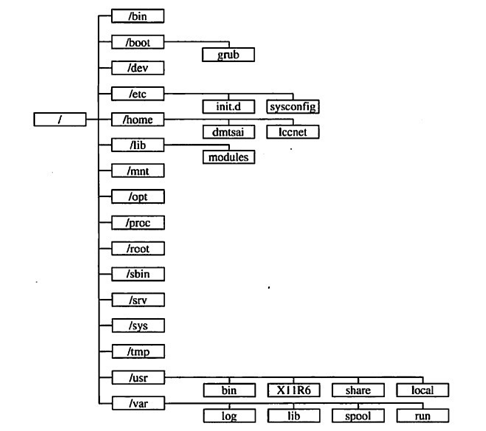
\includegraphics{images/linux-fs-tree.png}
\caption{Linux系统目录结构图}
\end{figure}

常用文件夹说明。

\begin{itemize}
\tightlist
\item
  \passthrough{\lstinline!/!} ------
  根目录,一般根目录下只存放目录,不要存放文件。/etc、/bin、/dev、/lib、/sbin应该和根目录放置在一个分区中。
\item
  \passthrough{\lstinline!/bin!} ------
  存放系统中最常用的二进制可执行文件(二进制文件)。基础系统所需要的那些命令位于此目录,也是最小系统所需要的命令;例如ls、cp、mkdir等命令。功能和/usr/bin类似,这个目录中的文件都是可执行的,普通用户都可以使用命令
\item
  \passthrough{\lstinline!/boot!} ------
  存放Linux内核和系统启动文件,包括Grub、lilo启动程序
\item
  \passthrough{\lstinline!/dev!} ------
  存放所有设备文件,包括硬盘、分区、键盘、鼠标、USB等
\item
  \passthrough{\lstinline!/etc!} ------
  存放系统所有配置文件,例如passwd存放用户账户信息,hostname存放主机名等。/etc/fstab是开机自动挂载一些分区的,在里面写入一些分区信息,就能实现开机挂载分区
\item
  \passthrough{\lstinline!/home!} ------ 用户目录的默认位置
\item
  \passthrough{\lstinline!/initrd!} ------
  存放启动时挂载initrd.img映像文件的目录,以及载入所需设备模块的目录
\item
  \passthrough{\lstinline!/lib!} ------
  存放共享的库文件,包含许多被/bin和/sbin中程序使用的库文件
\item
  \passthrough{\lstinline!/lost+found!} ------
  在ext2或者ext3文件系统中,当系统意外崩溃或者计算机意外关机,而产生一些文件碎片存放在这里。当系统启动的过程中fsck工具会检查这里,并修复已经损坏的文件系统。有时系统发生问题,有很多的文件被移动到这个目录中,可能会用手工的方式来修复或移动到文件的原位置上
\item
  \passthrough{\lstinline!/media!} ------
  即插即用型设备的挂载点自动在这个目录下创建。例如USB自动挂载后会在这个目录下产生一个目录;CDROM/DVD自动挂载后,也会在这个目录中创建一个目录,存放临时读入的文件
\item
  \passthrough{\lstinline!/mnt!} ------
  此目录通常用于作为被挂载的文件系统的挂载点
\item
  \passthrough{\lstinline!/proc!} ------
  存放所有标志为文件的进程,它们是通过进程号或其他的系统动态信息进行标识。例如CPU、硬盘分区、内存信息等存放在这里
\item
  \passthrough{\lstinline!/opt!} ------
  作为可选文件和程序的存放目录。有些软件包也会被安装在这里,也就是自定义软件包;有些用户自己编译的软件包,就可以安装在这个目录中
\item
  \passthrough{\lstinline!/root!} ------ 根用户(超级用户)的主目录
\item
  \passthrough{\lstinline!/sbin!} ------
  大多是涉及系统管理的命令的存放地,也是超级权限用户root的可执行命令存放地。普通用户无权限执行这个目录下的命令,这个目录和/usr/sbin;
  /usr/X11R6/sbin或/usr/local/sbin目录是相似的。注意,凡是目录sbin中包含的都是root权限才能执行的
\item
  \passthrough{\lstinline!/srv!} ------ 存放系统所提供的服务数据
\item
  \passthrough{\lstinline!/sys!} ------
  该目录用于将系统设备组织或层次结构,并向用户提供详细的内核数据信息
\item
  \passthrough{\lstinline!/tmp!} ------
  临时文件目录,有时用户运行程序的时候,会产生临时文件。/var/tmp目录和这个目录相似
\item
  \passthrough{\lstinline!/usr!} ------
  用于存放与系统用户直接有关的文件和目录,如应用程序及支出系统的库文件

  \begin{itemize}
  \tightlist
  \item
    \passthrough{\lstinline!/usr/X11R6!} ------ X Window系统
  \item
    \passthrough{\lstinline!/usr/bin!} ------ 用户管理员的标准命令
  \item
    \passthrough{\lstinline!/usr/include!} ------
    C/C++等开发工具语言环境的标准include文件
  \item
    \passthrough{\lstinline!/usr/lib!} ------ 应用程序及程序报的链接库
  \item
    \passthrough{\lstinline!/usr/local!} ------ 系统管理员安装的应用程序
  \item
    \passthrough{\lstinline!/usr/local/share!} ------
    系统管理员安装的共享文件
  \item
    \passthrough{\lstinline!/usr/sbin!} ------ 用户和管理员的标准命令
  \item
    \passthrough{\lstinline!/usr/share!} ------
    存放使用手册等共享文件的地方
  \item
    \passthrough{\lstinline!/usr/share/dict!} ------ 存放词表的目录
  \item
    \passthrough{\lstinline!/usr/share/man!} ------ 系统使用手册
  \item
    \passthrough{\lstinline!/usr/share/misc!} ------ 一般数据
  \item
    \passthrough{\lstinline!/usr/share/sgml!} ------ SGML数据
  \item
    \passthrough{\lstinline!/usr/share/xml!} ------ XML数据
  \end{itemize}
\item
  \passthrough{\lstinline!/var!} ------
  通常用于存放长度可变的文件,例如日志文件和打印机文件

  \begin{itemize}
  \tightlist
  \item
    \passthrough{\lstinline!/var/cache!} ------ 应用程序缓存目录
  \item
    \passthrough{\lstinline!/var/crash!} ------ 系统错误信息
  \item
    \passthrough{\lstinline!/var/games!} ------ 游戏数据
  \item
    \passthrough{\lstinline!/var/lib!} ------ 各种状态数据
  \item
    \passthrough{\lstinline!/var/lock!} ------ 文件锁定记录
  \item
    \passthrough{\lstinline!/var/log!} ------ 日志记录
  \item
    \passthrough{\lstinline!/var/mail!} ------ 电子邮件
  \item
    \passthrough{\lstinline!/var/opt!} ------
    \passthrough{\lstinline!/opt!}目录的变量数据
  \item
    \passthrough{\lstinline!/var/run!} ------ 进程的标示数据
  \item
    \passthrough{\lstinline!/var/spool!} ------
    存放电子邮件,打印任务等的队列目录
  \item
    \passthrough{\lstinline!/var/tmp!} ------ 临时文件目录
  \end{itemize}
\end{itemize}

\section{文件系统常用命令}

\begin{longtable}[]{@{}ll@{}}
\caption{文件系统常用命令}\tabularnewline
\toprule
\begin{minipage}[b]{0.16\columnwidth}\raggedright
\textbf{命令}\strut
\end{minipage} & \begin{minipage}[b]{0.78\columnwidth}\raggedright
\textbf{解释}\strut
\end{minipage}\tabularnewline
\midrule
\endfirsthead
\toprule
\begin{minipage}[b]{0.16\columnwidth}\raggedright
\textbf{命令}\strut
\end{minipage} & \begin{minipage}[b]{0.78\columnwidth}\raggedright
\textbf{解释}\strut
\end{minipage}\tabularnewline
\midrule
\endhead
\begin{minipage}[t]{0.16\columnwidth}\raggedright
\passthrough{\lstinline!cd!}\strut
\end{minipage} & \begin{minipage}[t]{0.78\columnwidth}\raggedright
改变目录\strut
\end{minipage}\tabularnewline
\begin{minipage}[t]{0.16\columnwidth}\raggedright
\passthrough{\lstinline!pwd!}\strut
\end{minipage} & \begin{minipage}[t]{0.78\columnwidth}\raggedright
显示当前目录\strut
\end{minipage}\tabularnewline
\begin{minipage}[t]{0.16\columnwidth}\raggedright
\passthrough{\lstinline!mkdir!}\strut
\end{minipage} & \begin{minipage}[t]{0.78\columnwidth}\raggedright
创建文件夹\strut
\end{minipage}\tabularnewline
\begin{minipage}[t]{0.16\columnwidth}\raggedright
\passthrough{\lstinline!chmod!}\strut
\end{minipage} & \begin{minipage}[t]{0.78\columnwidth}\raggedright
修改文件(夹)权限\strut
\end{minipage}\tabularnewline
\begin{minipage}[t]{0.16\columnwidth}\raggedright
\passthrough{\lstinline!ls!}\strut
\end{minipage} & \begin{minipage}[t]{0.78\columnwidth}\raggedright
列出文件夹内容\strut
\end{minipage}\tabularnewline
\bottomrule
\end{longtable}

下面给出几个简单例子。

\begin{lstlisting}[language=bash]
$ cd
$ cd ~
$ cd /usr/local/bin
$ cd -
$ cd ..
$ pwd
\end{lstlisting}

\textbf{解释}

\begin{enumerate}
\def\labelenumi{\arabic{enumi}.}
\tightlist
\item
  \passthrough{\lstinline!cd!}
  输入不带参数,默认是回到自己的主目录,也即\passthrough{\lstinline!\~!}目录,第一行第二行效果是一样的。
\item
  \passthrough{\lstinline!cd!}
  输入带一个目录,则跳转到该目录,如果你没有权限,则跳转失败。
\item
  \passthrough{\lstinline!-!}短横线表示上一个目录,也就是旧目录,方便你在两个目录之间切换。
\item
  \passthrough{\lstinline!cd!}
  输入的目录支持相对路径和绝对路径。\passthrough{\lstinline!..!}表示上级目录或者叫父目录,\passthrough{\lstinline!.!}表示当前目录,对于\passthrough{\lstinline!/!}根目录,其父目录就是他本身。
\item
  \passthrough{\lstinline!pwd!}打印当前目录。
\end{enumerate}

\begin{lstlisting}[language=bash]
$ cd
$ mkdir dir1
$ mkdir -p dir2/dir22
$ ls -ld dir1
drwxr-xr-x 2 litianci litianci 4096 10月 31 22:24 dir1
$ chmod o-rx dir1
$ touch dir1
$ ls -ld dir1
drwxr-x--- 2 litianci litianci 4096 10月 31 23:22 dir1
\end{lstlisting}

\textbf{解释}

\begin{enumerate}
\def\labelenumi{\arabic{enumi}.}
\tightlist
\item
  \passthrough{\lstinline!cd!}
  到主目录。使用\passthrough{\lstinline!mkdir!}新建一个文件夹。如果你想创建嵌套的文件夹,或者多层文件夹,可以使用\passthrough{\lstinline!mkdir -p!}选项,这样就可以建立多层文件夹。
\item
  \passthrough{\lstinline!ls -ld dir1!},\passthrough{\lstinline!-d!}选项,表示只显示文件夹本身,\passthrough{\lstinline!-l!}是列出详细信息。\passthrough{\lstinline!drwxr-xr-x!}表示:\passthrough{\lstinline!d!}该文件是个文件夹,\passthrough{\lstinline!rwxr-xr-x!}是该文件夹的权限。见后面详述。\passthrough{\lstinline!2!}表示其内部有2个子文件(夹),从上面的命令可以知道其实\passthrough{\lstinline!dir1!}是一个空文件夹,怎么会有两个子文件(夹)呢,其实是隐藏的\passthrough{\lstinline!..!}和\passthrough{\lstinline!.!}文件夹。你可以使用
  \passthrough{\lstinline!ls -la dir1!}看到这连个文件夹。后面依次为本文件(夹)的用户、用户组、文件大小,修改日期和时间。最后是本文件名称。
\item
  使用\passthrough{\lstinline!chmod!}命令,去除其他用户的读和执行权限(\passthrough{\lstinline!-rx!})
\item
  使用\passthrough{\lstinline!touch!}命令,修改\passthrough{\lstinline!dir1!}的\textbf{修改日期}。
\item
  再次使用\passthrough{\lstinline!ls -ld dir1!}命令,会发现相关的数值发生了变化。
\end{enumerate}

\section{元字符和操作符}

古人云\cqh 物以类聚,人以群分\cqt 。我们操作文件(夹)的时候,可能就需要批量操作。这个时候我们就可以这些文件(夹)\cqh 归类\cqt ,其实就是使用元字符表示某一类文件(夹)。这样操作起来更方便。

如果说元字符是对文件夹\cqh 分类\cqt ,那么操作符就是对\cqh 操作\cqt 按照一定的规则拼接。

\hypertarget{filesystem:metachar}{%
\subsection{元字符}\label{filesystem:metachar}}

常用的元字符有如下三种方式。

\begin{itemize}
\tightlist
\item
  \passthrough{\lstinline!*!}
  匹配任意数目的字符,跟正则表达式的\passthrough{\lstinline!*!}有所区别。
\item
  \passthrough{\lstinline!?!} 匹配一个字符,一个汉字也是作为一个字符。
\item
  \passthrough{\lstinline![...]!}
  匹配\passthrough{\lstinline![]!}内的任意一个字符,支持短横线\passthrough{\lstinline!-!}表示连续的字符。一个汉字也是作为一个字符。
\end{itemize}

看下面例子,

\begin{lstlisting}[language=bash]
$ mkdir test
$ cd test
$ touch huawei huashuo 华为 华硕 深度 深不可测
$ ls h*
huashuo  huawei
$ ls 华*
华硕  华为
$ ls 深*测
深不可测
\end{lstlisting}

\textbf{解释}

\begin{enumerate}
\def\labelenumi{\arabic{enumi}.}
\tightlist
\item
  第1-3行,创建空的文件夹\passthrough{\lstinline!test!},并转到该文件夹,创建了\passthrough{\lstinline!huawei!}等六个文件。
\item
  第4、6、8行,使用元字符\passthrough{\lstinline!*!}表示任意数目的字符,分别显示了匹配相关''分类``的文件。
\end{enumerate}

下面紧接着上面的shell环境,继续例子,

\begin{lstlisting}[language=bash]
$ ls h?????
huawei
$ ls 华?
华硕  华为
$ ls 深?
深度
\end{lstlisting}

\textbf{解释}

\begin{enumerate}
\def\labelenumi{\arabic{enumi}.}
\tightlist
\item
  第1行,可以看出每个\passthrough{\lstinline!?!}代表一个字符。
\item
  第3、5行,可以看出一个汉字算作一个字符。
\end{enumerate}

下面我们看看\passthrough{\lstinline![...]!}相关的例子,

\begin{lstlisting}[language=bash]
$ touch auawei buawei cuawei duawei
$ ls [ah]uawei
auawei  huawei
$ ls [a-dh]uawei
auawei  buawei  cuawei  duawei  huawei
$ ls [a-dh]u*
auawei  buawei  cuawei  duawei  huashuo  huawei
\end{lstlisting}

\textbf{解释}

\begin{enumerate}
\def\labelenumi{\arabic{enumi}.}
\tightlist
\item
  第1行,为了方便演示,我新建了四个文件。
\item
  第2行,\passthrough{\lstinline![ah]uawei!}表示,\passthrough{\lstinline!a!}和\passthrough{\lstinline!h!}任选一个,后面紧挨着\passthrough{\lstinline!uawei!}。匹配的字符见第3行显示结果。
\item
  第4行,我们可以看出短横线\passthrough{\lstinline!-!}的意思,表示一个序列。也支持数字的连续显示,但是只支持个位数,\textbf{是否如此请核实}。
\item
  第6行,其实这些元字符可以配合使用。
\end{enumerate}

\subsection{操作符}

本节内容见第\ref{sec:redirect}小节。本节从略。

\subsection{\texorpdfstring{花括号\texttt{\{\}}}{花括号\{\}}}

第@ref(\url{filesystem:metachar)小节提到的均为归类,前提是筛选,选择已经存在的事物,对已有的事情分类}(\textbf{是否如此请核实})。如果你想创建一个集合,可以选择花括号\passthrough{\lstinline!\{\}!}的方式,列出所有相关的元素。

\begin{lstlisting}[language=bash]
$ touch deepin{1,2,3,4}
$ ls deepin*
deepin1  deepin2  deepin3  deepin4
$ rm ./*
$ touch {deepin,深度}-{5,6,7,8}
$ ls
deepin-5  deepin-6  deepin-7  deepin-8  深度-5  深度-6  深度-7  深度-8
$ rm {deepin,深度}-{5,6,7,8}
$ ls
$ touch {a..e}{1..3}
$ ls
a1  a2  a3  b1  b2  b3  c1  c2  c3  d1  d2  d3  e1  e2  e3
$ rm ./*
$ touch {A..a}
touch: 无法创建'': 没有那个文件或目录
$ ls
'`'   _    ]   A   C   E   G   I   K   M   O   Q   S   U   W   Y
'^'  '['   a   B   D   F   H   J   L   N   P   R   T   V   X   Z
$ rm ./*
$ touch {aa..ac}
$ ls
{aa..ac}
$ rm ./*
$ touch {11..21}
$ ls
11  12  13  14  15  16  17  18  19  20  21
$ rm ./*
$ touch {33..22}
$ touch {z..b}
\end{lstlisting}

\textbf{解释}

\begin{enumerate}
\def\labelenumi{\arabic{enumi}.}
\tightlist
\item
  第1行,创建了\passthrough{\lstinline!deepin!}开头,以后面集合元素结尾的文件。
\item
  第5行,集合拼接在一起,类似于笛卡尔积的形式组合起来。
\item
  第10行,对于单字母支持序列功能,多字母则不支持。对于数字支持序列功能。按照ASCII码排序,从\passthrough{\lstinline!A!}到\passthrough{\lstinline!a!}包含不显示的字符,影响最终的显示。
\item
  最后两行,没有显示结果,有兴趣的读者可以使用\passthrough{\lstinline!ls!}看看结果。
\end{enumerate}

\section{几个常用的目录}

\begin{itemize}
\tightlist
\item
  \passthrough{\lstinline!$HOME!} 主目录
\item
  \passthrough{\lstinline!\~!}
  波浪线,位于键盘左上角第二行开头的那个键(按下的时候需要按\passthrough{\lstinline!shift!}键),也是表示主目录,为了跳转到其他人的主目录,也可用使用\passthrough{\lstinline!\~<username>!}的方式。比如跳转到\passthrough{\lstinline!litianci!}的主目录,\passthrough{\lstinline!cd \~litianci!}
\item
  \passthrough{\lstinline!-!} 或者
  \passthrough{\lstinline!$OLDPWD!},表示上一个目录,这个是短横线,不是减号。如果你在两个目录之间切换的话,\passthrough{\lstinline!cd -!}方便你跳转,如果你还没有切换目录,跳转到旧目录则会报错。\passthrough{\lstinline!-!}还有其他的功能,比如放权当前环境切换到新用户,\passthrough{\lstinline!sudo su -!},这个命令就是不管你现在处于什么目录,切换到\passthrough{\lstinline!root!}根用户,且工作目录为\passthrough{\lstinline!root!}根用户的主目录。
\item
  \passthrough{\lstinline!.!} 或 \passthrough{\lstinline!$PWD!}
  当前工作目录。这两者是否有区别,待查。
\item
  \passthrough{\lstinline!..!}
  上级目录,也即父目录。对于\passthrough{\lstinline!/!}根目录而言,\passthrough{\lstinline!..!}和\passthrough{\lstinline!.!}都表示本级目录。
\end{itemize}

\section{文件(夹)的权限和归属}

Linux
是多用户的系统,为了在一定程度上保护数据隐私,对文件(夹)进行简单的权限控制。这也是你输入命令或者做其他事情的时候会遇到的没有权限问题的根源,甚至部分用户喜欢用\passthrough{\lstinline!root!}根用户操作,也是因为权限控制造成的某些不方便。为了更好的用权,也为了数据的安全,还请能用普通用户的情况下,尽量少用\passthrough{\lstinline!root!}根用户操作。下面对权限进行简要介绍。

对于一个文件(夹)来说,他一定归属于某个用户,且归属于某个用户组。也一定有其他不属于前两者的用户,简称其他用户,有时候也想访问该文件(夹)。那么这个权限就是针对这三类人来设定的。当然,由于某些用户(组)被删除等,造成文件(夹)归属的用户(组)不存在了,这些就是无主文件(夹),这也是存在安全隐患的。在下章内容会讲述通过\passthrough{\lstinline!find!}命令查找此类无主文件(夹)的方法,可以采用相关方法,重新赋予其归属用户(组)或者删除等,这里就不叙述了。

\subsection{权限简介}

参考网页:

\begin{itemize}
\tightlist
\item
  \url{https://blog.csdn.net/zhao12795969/article/details/53448039}
\end{itemize}

针对这三类用户,权限又可以分为读(Read)、写(Write)和执行(eXecute)三类。

\begin{itemize}
\tightlist
\item
  r(Read,读取):对文件而言,具有读取文件内容的权限;对目录来说,具有浏览目录的权限。
\item
  w(Write,写入):对文件而言,具有新增,修改,删除文件内容的权限;对目录来说,具有新建,删除,修改,移动目录内文件的权限。
\item
  x(eXecute,执行):对文件而言,具有执行文件的权限;对目录了来说该用户具有进入目录的权限。
\end{itemize}

\textbf{注意}

\begin{enumerate}
\def\labelenumi{\arabic{enumi}.}
\tightlist
\item
  目录的只读访问不允许使用cd进入目录,必须要有执行的权限才能进入。
\item
  只有执行权限只能进入目录,不能看到目录下的内容,要想看到目录下的文件名和目录名,需要可读权限。
\item
  一个文件能不能被删除,主要看该文件所在的目录对用户是否具有写权限,如果目录对用户没有写权限,则该目录下的所有文件都不能被删除,文件所有者除外。
\item
  目录的w位不设置,即使你拥有目录中某文件的w权限也不能写该文件。
\item
  以上仅限于
  \passthrough{\lstinline!ext3/4!}等文件系统的文件。对于安装\passthrough{\lstinline!windows10!}双系统的电脑,还需要注意是否\passthrough{\lstinline!windows10!}开启电源保护模式,哪怕你是\passthrough{\lstinline!ext4!}格式,依旧为只读,无法更改文件。
\end{enumerate}

每个文件属于一个用户和一个组。命令\passthrough{\lstinline!ls -l!}可以查看用户和组,比如,

\begin{lstlisting}[language=bash]
$ ls -l /bin/bash 
-rwxr-xr-x 1 root root 1111240 5月  13  2018 /bin/bash
\end{lstlisting}

第二行为输出结果,表明 \passthrough{\lstinline!/bin/bash!} 属于 root
用户, root 组。\passthrough{\lstinline!ls -l!} 命令的第一个字段
\passthrough{\lstinline!-rwxr-xr-x!}
包含\passthrough{\lstinline!/bin/bash!}的权限的符号表示。该字段中的首字符(\passthrough{\lstinline!-!})指定该文件的类型,本例中它是一个常规文件。可能的首字符如下:

\begin{itemize}
\tightlist
\item
  \passthrough{\lstinline!-!} 普通文件
\item
  \passthrough{\lstinline!d!} 目录
\item
  \passthrough{\lstinline!l!} 符号链接
\item
  \passthrough{\lstinline!c!} 字符专门设备文件
\item
  \passthrough{\lstinline!b!} 块专门设备文件
\item
  \passthrough{\lstinline!p!} 先进先出
\item
  \passthrough{\lstinline!s!} 套接字
\end{itemize}

首字符后紧接着三个三元组\passthrough{\lstinline!rwx!},\passthrough{\lstinline!r-x!},\passthrough{\lstinline!r-x!},第一个三元字符组代表文件所有者的权限,第二个代表文件的所属组的权限,第三个代表其他用户的权限。但是
root 用户,往往会被跳过这些权限检查(\textbf{待核实})。

\hypertarget{chmod}{%
\subsection{\texorpdfstring{权限更改\texttt{chmod}}{权限更改chmod}}\label{chmod}}

\passthrough{\lstinline!chmod!} 用于更改 \passthrough{\lstinline!rwx!}
权限,带有两个或多个参数:\passthrough{\lstinline!mode!},描述怎样改变权限,后面跟将会受到影响的文件或文件列表:

\begin{lstlisting}[language=bash]
$ chmod +x bashscript
\end{lstlisting}

上例\passthrough{\lstinline!+x!}表示对\passthrough{\lstinline!bashscript!}的三类人员(拥有者、拥有组和其他人)均增加可执行权限。如果我们想要除去一个文件的所有执行权限,

\begin{lstlisting}[language=bash]
$ chmod -x bashscript
\end{lstlisting}

为了更精细的控制权限,比如只修改部分人员权限,需要在\passthrough{\lstinline!+-!}符号前加上这部分人员的代号。\passthrough{\lstinline!a!}表示所有人员,\passthrough{\lstinline!u!}表示拥有者,\passthrough{\lstinline!g!}表示拥有组,\passthrough{\lstinline!o!}表示其他人员。这些代号可以合用。比如下面这行命令表示组和其他人员去除读写权限增加执行权限。

\begin{lstlisting}[language=bash]
$ chmod go-rw+x bashscript
\end{lstlisting}

对于权限,除了\passthrough{\lstinline!+-!}外,还可以使用等号\passthrough{\lstinline!=!},表示只保留这些权限,未涉及的权限全部取消,有例外,见下文。

\begin{lstlisting}[language=bash]
$ chmod =rx bashscript
\end{lstlisting}

\textbf{注意}

使用\passthrough{\lstinline!+-=!}改变权限的时候,最好在前面加上相关人员的代号,比如\passthrough{\lstinline!a!},\passthrough{\lstinline!u!},\passthrough{\lstinline!g!},\passthrough{\lstinline!o!}的组合,否则,可能跟你预期的结果不一样。

\begin{lstlisting}[language=bash]
$ chmod a-rwx bashscript
$ chmod +rwx bashscript # + 不一定跟你期望的一样
$ ls -l bashscript # rwxr-xr-x
$ chmod a-rwx bashscript
$ chmod a+rwx bashscript
$ ls -l bashscript # rwxrwxrwx
$ chmod -rwx bashscript # - 不一定跟你期望的一样
$ ls -l bashscript # ----w--w-
$ chmod a-rwx bashscript
$ ls -l bashscript # ---------
$ chmod =rwx bashscript
$ ls -l bashscript # rwxr-xr-x
\end{lstlisting}

以上是因为存在权限掩码\passthrough{\lstinline!umask!}这个参数,在终端输入\passthrough{\lstinline!umask!}回车,输出本机\passthrough{\lstinline!umask=0022!},怎么是数字呢?这是因为权限也可用用数字表示,关于权限掩码\passthrough{\lstinline!umask!}在后面详述。

数字形式的权限,使用4位八进制数,每一位代表一个权限三元组。例如,在
\passthrough{\lstinline!1777!} 中,\passthrough{\lstinline!777!}
设置本章我们所讨论的\passthrough{\lstinline!owner!}、\passthrough{\lstinline!group!}和\passthrough{\lstinline!other!}标志。\passthrough{\lstinline!1!}
用来设置专门的权限位,稍后再讲。这个图表说明了怎样解释第二到

: 字符形式权限和数字形式权限对照表

\begin{longtable}[]{@{}cccccccc@{}}
\toprule
\textbf{字符} & \textbf{数字} & \textbf{字符} & \textbf{数字} &
\textbf{字符} & \textbf{数字} & \textbf{字符} &
\textbf{数字}\tabularnewline
\midrule
\endhead
\passthrough{\lstinline!rwx!} & 7 & \passthrough{\lstinline!rw-!} & 6 &
\passthrough{\lstinline!r-x!} & 5 & \passthrough{\lstinline!r--!} &
4\tabularnewline
\passthrough{\lstinline!-wx!} & 3 & \passthrough{\lstinline!-w-!} & 2 &
\passthrough{\lstinline!--x!} & 1 & \passthrough{\lstinline!---!} &
0\tabularnewline
\bottomrule
\end{longtable}

采用数字形式的权限管理方法,比如,

\begin{lstlisting}[language=bash]
$ chmod 0755 bashscript
$ ls -l bashscript
-rwxr-xr-x 1 litianci litianci 119 11月 17 22:32 bashscript
\end{lstlisting}

就实现跟字符形式等同的权限设置。

\hypertarget{umask}{%
\subsection{\texorpdfstring{权限掩码\texttt{umask}}{权限掩码umask}}\label{umask}}

当进程创建了新文件时,它指定新文件应该具有的权限。通常,所请求的模式是
0666(每个人可读和可写),它比我们希望的具有更多的权限。幸运的是,不管什么时候创建了新文件,Linux
将参考叫做权限掩码\passthrough{\lstinline!umask!}的东西。系统用\passthrough{\lstinline!umask!}值来将初始指定的权限降低为更合理、更安全的权限。您可以通过在命令行中输入\passthrough{\lstinline!umask!}来查看您当前的\passthrough{\lstinline!umask!}设置,

\begin{lstlisting}[language=bash]
$ umask
0022
\end{lstlisting}

Linux 系统上,\passthrough{\lstinline!umask!} 的缺省值一般为
\passthrough{\lstinline!0022!},它允许其他人读您的新文件(如果他们可以得到它们),但是不能进行修改。为了在缺省的情况下使新文件更安全,您可以改变
\passthrough{\lstinline!umask!} 设置,

\begin{lstlisting}[language=bash]
$ umask 0077
$ touch newfile # 新建一个文件
$ ls -l newfile
-rw------- 1 litianci litianci 0 11月 21 18:39 newfile
\end{lstlisting}

\passthrough{\lstinline!umask!}
将确保组和其他用户对于新创建的文件绝对没有任何权限。参阅上方的《字符形式权限和数字形式权限对照表》,当\passthrough{\lstinline!umask=0077!}时,对应字符形式权限为
\passthrough{\lstinline!---rwxrwx!}。而新建文件的请求权限为\passthrough{\lstinline!0666!}(\passthrough{\lstinline!rw-rw-rw-!}),禁用掉\passthrough{\lstinline!0077!}后,就剩上方显示的\passthrough{\lstinline!rw-------!}权限了。

\hypertarget{suid--sgid}{%
\subsubsection{\texorpdfstring{\texttt{suid} 和
\texttt{sgid}}{suid 和 sgid}}\label{suid--sgid}}

当您最初登录时,将启动一个新的 shell 进程。这个新的 shell 进程(通常是
bash)使用您的用户标识运行,可以访问所有属于您的文件(夹)。您启动的程序继承了您的用户标识,因此它们不能访问任何不允许您访问的文件系统对象。例如,一般用户不能直接修改
\emph{/etc/passwd}
文件,因为\passthrough{\lstinline!write!}标志已经对除\passthrough{\lstinline!root 用户!}以外的每个用户关闭,

\begin{lstlisting}[language=bash]
$ ls -l /etc/passwd
-rw-r--r-- 1 root root 2438 11月 21 15:54 /etc/passwd
\end{lstlisting}

但是,一般用户确实需要在他们需要改变其密码的任何时候,能够修改
\emph{/etc/passwd}(至少间接地)。但是,如果用户不能修改该文件,究竟怎样完成这个工作呢?

幸好,Linux
权限模型有两个专门的位,叫做\passthrough{\lstinline!suid!}和\passthrough{\lstinline!sgid!}。当设置了一个可执行程序的\passthrough{\lstinline!suid!}这一位时,它将代表可执行文件的所有者运行,而不是代表启动程序的人运行。现在回到上面这个问题。查看
\emph{/usr/bin/passwd} 可执行文件,

\begin{lstlisting}[language=bash]
$ ls -l /usr/bin/passwd
-rwsr-xr-x 1 root root 59640 9月  28  2017 /usr/bin/passwd
\end{lstlisting}

您还将注意到,这里有一个 \passthrough{\lstinline!s!}
取替了用户权限三元组中的一个
\passthrough{\lstinline!x!}。这表明,对于这个特殊程序,设置了
\passthrough{\lstinline!suid!} 和可执行位。由于这个原因,当
\passthrough{\lstinline!/usr/bin/passwd!} 运行时,它将代表 root
用户执行(具有完全超级用户访问权),而不是代表运行它的用户运行。又因为
\passthrough{\lstinline!/usr/bin/passwd!} 以 root
用户访问权运行,所以能够修改 \emph{/etc/passwd} 文件,而没有什么问题。

我们看到了 \passthrough{\lstinline!suid!}
怎样工作,\passthrough{\lstinline!sgid!}
以同样的方式工作。它允许程序继承程序的组所有权,而不是当前用户的组所有权。

这里有一些关于 \passthrough{\lstinline!suid!} 和
\passthrough{\lstinline!sgid!} 的其它的但是很重要的信息。

首先,\passthrough{\lstinline!suid!} 和 \passthrough{\lstinline!sgid!}
分别占据与 \passthrough{\lstinline!ls -l!}
清单中用户\passthrough{\lstinline!u!}和用户组\passthrough{\lstinline!g!}的执行\passthrough{\lstinline!x!}位。如果设置了
\passthrough{\lstinline!x!} 位为可执行,则相应的位表示为
\passthrough{\lstinline!s!}(小写)否则为
\passthrough{\lstinline!S!}(大写)。

其次,在许多环境中,\passthrough{\lstinline!suid!} 和
\passthrough{\lstinline!sgid!}
很管用,但是不恰当地使用这些位可能使系统的安全遭到破坏。最好尽可能地少用\passthrough{\lstinline!suid!}程序。\passthrough{\lstinline!/usr/bin/passwd!}
命令是为数不多的必须使用\passthrough{\lstinline!suid!}的命令之一。

设置和除去 \passthrough{\lstinline!suid!} 与
\passthrough{\lstinline!sgid!} 位相当简单。这里,我们设置 suid 位:

\begin{lstlisting}[language=bash]
$ ls -l bashscript 
-rwxr-xr-x 1 litianci litianci 119 11月 17 22:32 bashscript
$ chmod u+s bashscript 
$ ls -l bashscript 
-rwsr-xr-x 1 litianci litianci 119 11月 17 22:32 bashscript
$ chmod u-x bashscript 
$ ls -l bashscript 
-rwSr-xr-x 1 litianci litianci 119 11月 17 22:32 bashscript
$ chmod g+s bashscript 
$ ls -l bashscript 
-rwSr-sr-x 1 litianci litianci 119 11月 17 22:32 bashscript
$ chmod g-s bashscript 
$ ls -l bashscript 
-rwSr-xr-x 1 litianci litianci 119 11月 17 22:32 bashscript
\end{lstlisting}

权限和目到此为止,我们从常规文件的角度来看权限。当从目录的角度看权限时,情况有一点不同。目录使用同样的权限标志,但是它们被解释为表示略微不同的含义。
对于一个目录,如果设置了\passthrough{\lstinline!read!}标志,您可以列出目录的内容;\passthrough{\lstinline!write!}表示您可以在目录中创建文件,\passthrough{\lstinline!execute!}表示您可以进入该目录并访问内部的任何子目录。没有\passthrough{\lstinline!execute!}标志,目录内的文件系统对象是不可访问的。没有\passthrough{\lstinline!read!}标志,目录内的文件系统对象是不可查看的,但是只要有人知道磁盘上对象的完整路径,就仍然可以访问目录内的对象。

如果启用了目录的\passthrough{\lstinline!sgid!}标志,在目录内创建的任何文件系统对象将继承目录的组。当您需要创建一个属于同一组的一组人使用的目录树时,这种特殊的功能很管用。只需要这样做,

\begin{lstlisting}[language=bash]
$ mkdir -p /media/litianci/data/groupspace
$ sudo chgrp mygroup /media/litianci/data/groupspace
$ chmod g+s /media/litianci/data/groupspace
\end{lstlisting}

现在,mygroup 组中的所有用户都可以在
\emph{/media/litianci/data/groupspace}
内创建文件或目录,同样,他们也将自动地分配到 mygroup
的组所有权。根据用户的 \passthrough{\lstinline!umask!}
设置,新文件系统对象对于 mygroup
组的其他成员来说,可以或不可以是可读、可写或可执行的。

\subsubsection{目录和删除}

缺省情况下,Linux
目录以一种不是在所有情况下都很理想的方式表现。一般来说,只要对一个目录有写访问权,任何人都可以重命名或删除该目录中的文件。对于个别用户使用的目录,这种行为是很合理的。

但是,对于很多用户使用的目录来说,尤其是 \emph{/tmp} 和
\emph{/var/tmp},这种行为可能会产生麻烦。因为任何人都可以写这些目录,任何人都可以删除或重命名任何其他人的文件------即使是不属于他们的!显然,当任何其他用户在任何时候都可以输入\passthrough{\lstinline!rm -rf /tmp/*!}并损坏每个人的文件时,很难在
\emph{/tmp} 存放任何有意义的文件。

所幸,Linux 提供了\cqh 粘滞位\cqt (sticky bit)的东西。当给 \emph{/tmp}
设置了粘滞位(用\passthrough{\lstinline!chmod +t!}),唯一能够删除或重命名
\emph{/tmp} 中文件的是该目录的所有者(通常是 root 用户)、文件的所有者或
root 用户。事实上,所有 Linux 分发包都缺省地启用了 \emph{/tmp}
的粘滞位,而您还可以发现粘滞位在其它情况下也很管用。很显然,\cqh 粘滞位\cqt 是属于其他类型人员的权限,跟\passthrough{\lstinline!suid!},\passthrough{\lstinline!sgid!}一样,占据的也是权限三元组的\passthrough{\lstinline!x!}位,小写是设置了执行权限,大写是禁用了执行权限。所不同的是他们分别占据\passthrough{\lstinline!u!},\passthrough{\lstinline!g!},\passthrough{\lstinline!o!}的\passthrough{\lstinline!x!}位。

\begin{lstlisting}[language=bash]
$ ls -dl /tmp
drwxrwxrwt 15 root root 4096 11月 22 10:19 /tmp
$ sudo chmod o-x /tmp
$ ls -dl /tmp
drwxrwxrwT 16 root root 4096 11月 22 10:25 /tmp
\end{lstlisting}

\subsubsection{数字形式权限的第一位数字}

现在我们回过头来看数字权限的第一位数字的意思,这也是一个八进制数字,\passthrough{\lstinline!0-7!},转化为三位的二进制数,从高位到低位,分别表示\passthrough{\lstinline!suid!},\passthrough{\lstinline!sgid!},\passthrough{\lstinline!sticky!}。当设置该权限时为\passthrough{\lstinline!1!},禁用该权限时为\passthrough{\lstinline!0!}。比如,\passthrough{\lstinline!3!}就表示,禁用\passthrough{\lstinline!suid!},启用\passthrough{\lstinline!sgid!},\passthrough{\lstinline!sticky!}。看下面例子。

\begin{lstlisting}[language=bash]
$ chmod 1777 bashscript 
$ ls -l bashscript 
-rwxrwxrwt 1 litianci litianci 119 11月 17 22:32 bashscript
$ chmod 2777 bashscript 
$ ls -l bashscript 
-rwxrwsrwx 1 litianci litianci 119 11月 17 22:32 bashscript
$ chmod 4777 bashscript 
$ ls -l bashscript 
-rwsrwxrwx 1 litianci litianci 119 11月 17 22:32 bashscript
\end{lstlisting}

\subsection{归属}

参考网页:

\begin{itemize}
\tightlist
\item
  \url{https://www.cnblogs.com/DawaTech/p/7249734.html}
\end{itemize}

语法结构如下,

\begin{lstlisting}[language=bash]
chgrp 组名 文件(夹) -R
chown 用户名 文件(夹) -R
\end{lstlisting}

其中\passthrough{\lstinline!chgrp!}表示改变组名;\passthrough{\lstinline!chown!}表示改变用户名;\passthrough{\lstinline!-R!}表示递归目录下所有文件,可略。\textbf{更改所属用户和所属组常常需要根用户权限。}

\hypertarget{chgrp}{%
\subsubsection{\texorpdfstring{修改文件所属组群\texttt{chgrp}}{修改文件所属组群chgrp}}\label{chgrp}}

\passthrough{\lstinline!chgrp!},就是change
group的缩写(我们可以利用这些来记忆命令)。看例子,

\begin{lstlisting}[language=bash]
[litianci]$ sudo groupadd groupa # 增加组 groupa
[litianci]$ sudo groupadd groupb # 增加组 groupb
[litianci]$ sudo useradd -g groupa deepin -m # 新增用户 deepin,默认组 groupa,自带主目录
[litianci]$ sudo su - deepin # 切换到 deepin 用户,- 表示不保存当前任何环境变量
[deepin]$ touch filea fileb # 创建两个文件
[deepin]$ ls -l
-rw-r--r-- 1 deepin groupa    0 11月 21 15:55 filea
-rw-r--r-- 1 deepin groupa    0 11月 21 15:55 fileb
[deepin]$ exit
[litianci]$ sudo chgrp groupb ~deepin/filea # 改变filea所属群组
[litianci]$ sudo ls -l ~deepin/
-rw-r--r-- 1 deepin groupb    0 11月 21 15:55 filea
-rw-r--r-- 1 deepin groupa    0 11月 21 15:55 fileb
\end{lstlisting}

由于新增用户权限的问题,后面使用其他用户(\passthrough{\lstinline!ls -l!})访问文件的属性。执行命令的用户放在每行命令的开头了。

\hypertarget{chown}{%
\subsubsection{\texorpdfstring{修改文件拥有者\texttt{chown}}{修改文件拥有者chown}}\label{chown}}

\passthrough{\lstinline!chown!},即change
owner改变归属用户。\passthrough{\lstinline!chown!}功能很多,不仅仅能更改文件拥有者,还可以修改文件所属组群。如果需要将某一目录下的所有文件都改变其拥有者,可以使用\passthrough{\lstinline!-R!}参数。

语法结构如下,

\begin{lstlisting}[language=bash]
chown [-R] 账号名称      文件/目录
chown [-R] 账号名称:组群  文件/目录
\end{lstlisting}

下面简单示例,

\begin{lstlisting}[language=bash]
$ touch demo
$ ls -l demo
-rw-r--r-- 1 litianci litianci 0 11月 21 16:13 demo
$ sudo chown deepin demo # 修改文件 demo 的拥有者为 deepin
$ ls -l demo
-rw-r--r-- 1 deepin litianci 0 11月 21 16:13 demo
$ sudo chown deepin:groupa demo # 修改 demo 的拥有者为 deepin,拥有组 groupa
-rw-r--r-- 1 deepin groupa 0 11月 21 16:13 demo
\end{lstlisting}

\section{文件(夹)的创建、查看、移动、复制和删除}

有点类似数据库的增删改查(CRUD,Create,Read,Update,Delete),这里只提到了文件(夹)的创建、查看、移动(包括重命名)、复制和删除。修改涉及到文件的权限以及日期等等内容,这里略过不提。

\subsection{文件(夹)的创建}

对于文件夹的创建,常用\passthrough{\lstinline!mkdir!}这个命令。具体方法,前面已经讲解了。对于文件的创建,通常使用\passthrough{\lstinline!touch!}创建文件,通过\passthrough{\lstinline!man touch!}可以看出,一般情况,\passthrough{\lstinline!touch!}只是对访问和更改的时间戳重置为当前时间戳,创建文件只是附带功能。另外一般的编辑器,还有其他文件都有新建保存功能,这样也可用创建文件。这里就不详细介绍了。

\subsection{文件(夹)的查看}

对于文件的内容查看,可以通过各种阅读器或者编辑器等,根据文件的类型做出不同选择。因为Unix哲学奉行\cqh 一切皆文件\cqt ,编辑器是一种比较常见的查看方式,这个见第\ref{chap:vim-find}章。

文件(夹)的查看,通常采用\textbf{深度文件管理器}。对于其属性,可以通过\textbf{深度文件管理器}右击找到属性来查看。当然在命令行下\passthrough{\lstinline!ls!}也是一个非常强大的存在。看下面的例子。

\begin{lstlisting}[language=bash]
$ ls
$ ls -la
$ ls -lR
\end{lstlisting}

\textbf{解释}

\begin{enumerate}
\def\labelenumi{\arabic{enumi}.}
\tightlist
\item
  \passthrough{\lstinline!ls!}的选项\passthrough{\lstinline!-a!}表示把当前包含隐藏文件(夹)在内的所有文件(夹)显示出来。
\item
  \passthrough{\lstinline!-R!}选项是递归显示,可以把各个子文件夹的内容也显示出来。\passthrough{\lstinline!-l!}的显示内容,见上面章节说明。更多内容,可以查看\passthrough{\lstinline!man ls!}。
  \#\#\# 文件(夹)的移动及重命名
\end{enumerate}

文件(夹)的移动和重命名是通过\passthrough{\lstinline!mv!}命令实现的。

\begin{lstlisting}[language=bash]
$ mv litianci deepin
$ mv deepin ~
$ mv test1 test2 test3 ~
$ mv ~/deepin-bible/ ~/test/
$ mv ~/Desktop/* ~/test/
\end{lstlisting}

\textbf{解释}

\begin{enumerate}
\def\labelenumi{\arabic{enumi}.}
\tightlist
\item
  第1行,对文件\passthrough{\lstinline!litianci!}重命名为
  \passthrough{\lstinline!deepin!}。\passthrough{\lstinline!mv!}重命名时,不区分文件夹或文件。
\item
  第2行,把文件
  \passthrough{\lstinline!deepin!}移动到\passthrough{\lstinline!\~!}文件夹。
\item
  第3行,\passthrough{\lstinline!mv!}支持多个文件同时移动到最后面一个文件夹。请注意,\textbf{当多个文件(夹)同时移动时,最后一个必须是文件夹或指向文件夹的链接}。
\item
  第4行,把文件夹\passthrough{\lstinline!deepin-bible!}文件夹,包括文件夹的内容(含隐藏内容),移动到\passthrough{\lstinline!\~/test/!}文件夹。
\item
  第5行,只是把文件夹\passthrough{\lstinline!Desktop!}内的非隐藏内容,移动到\passthrough{\lstinline!\~/test/!}文件夹。
\end{enumerate}

注意,默认的\passthrough{\lstinline!mv!},对于重名冲突是直接覆盖的。如果想不被覆盖,建议在\passthrough{\lstinline!\~/.bashrc!}内加上\passthrough{\lstinline!alias mv='mv -i'!},遇到这类的问题的时候,就会征询你的意见再决定要不要覆盖。

\subsection{文件(夹)的复制}

\begin{lstlisting}[language=bash]
$ cp litianci deepin
$ cp deepin ~
$ cp test1 test2 test3 ~
$ cp -r ~/deepin-bible/ ~/test/
$ cp -ra ~/Desktop/* ~/test/
\end{lstlisting}

\textbf{解释}

\begin{enumerate}
\def\labelenumi{\arabic{enumi}.}
\tightlist
\item
  第1-3行,类似\passthrough{\lstinline!mv!}命令,实现对文件的复制,不含文件夹的复制。
\item
  第4行,对于文件夹的复制,需要带\passthrough{\lstinline!-r!}选项,递归(\passthrough{\lstinline!recursive!})的意思。
\item
  第5行,复制\passthrough{\lstinline!-a!}选项,表示复制后的文件(夹)各时间戳和权限跟原文件(夹)一样。
\end{enumerate}

\subsection{文件(夹)的删除}

\begin{lstlisting}[language=bash]
$ rm deepin
$ rm ./-
$ rm *
$ rmdir /home/joe/nothing/
$ rm -r /home/joe/bigdir/
$ rm -rf /home/joe/hugedir/
$ sudo rm -rf / #千万不要试运行
\end{lstlisting}

\textbf{解释}

\begin{enumerate}
\def\labelenumi{\arabic{enumi}.}
\tightlist
\item
  第1行,普通文件可以直接删除。不支持文件夹直接删除。如果要删除文件夹见第4-6行。
\item
  第2行,对于特殊文件,比如\passthrough{\lstinline!-!},一般写绝对路径。
\item
  第3行,\passthrough{\lstinline!*!}一般代表的都是非隐藏文件(夹)。没有\passthrough{\lstinline!-r!}递归选项,也可用删除当前文件夹下的所有非隐藏内容。
\item
  第4行,删除文件夹的命令\passthrough{\lstinline!rmdir!},删除了\passthrough{\lstinline!nothing!}文件夹及其内容。
\item
  第5-6行,\passthrough{\lstinline!-r!}表示递归,可以使用\passthrough{\lstinline!rm!}删除文件夹。\passthrough{\lstinline!-f!}是强制删除,实际是不用询问直接删除,对于没有权限删除的,依旧无法删除。
\item
  第7行,千万不要试运行。但是有时候为了删除本文件夹下的内容,往往错输。
\end{enumerate}

我的建议是\passthrough{\lstinline!alias rm='trash-put'!},把删除改为放置到回收站。具体做法见附录\ref{chap:faqs}。

\hypertarget{-4}{%
\section{总结}\label{-4}}

本章介绍了Linux操作系统的文件结构,并对文件的权限和归属情况进行了介绍,最后对文件的改动复制等作了简要介绍。

\hypertarget{chap:vim-find}{%
\chapter{文件编辑与查找}\label{chap:vim-find}}

通过阅读本章,你将会了解到以下几项内容。

\begin{itemize}
\tightlist
\item
  字符集和字符编码
\item
  编辑器简介
\item
  文件查找
\end{itemize}

\section{字符集和字符编码}

参考网页:

\begin{itemize}
\tightlist
\item
  \url{https://baike.baidu.com/item/\%E5\%AD\%97\%E7\%AC\%A6\%E9\%9B\%86/946585?fr=aladdin}
\item
  \url{https://www.cnblogs.com/happyday56/p/4135845.html}
\item
  \url{https://linux.cn/article-7959-1.html}
\end{itemize}

提到文本文件,不得不说文件的字符集,对于英文世界,ASCII码足够他们玩耍的了,但是对于中文,我们还需要中文字符集,不然就会显示很多框框或者乱码等。

字符(Character)是各种文字和符号的总称,包括各国家文字、标点符号、图形符号、数字等。字符集(Character
set)是多个字符的集合,字符集种类较多,每个字符集包含的字符个数不同,常见字符集名称:ASCII字符集、GB2312字符集、BIG5字符集、
GB18030字符集、Unicode字符集等。计算机要准确的处理各种字符集文字,需要进行字符编码,以便计算机能够识别和存储各种文字。中文文字数目大,而且还分为简体中文和繁体中文两种不同书写规则的文字,而计算机最初是按英语单字节字符设计的,因此,对中文字符进行编码,是中文信息交流的技术基础。

\hypertarget{ascii}{%
\subsection{ASCII}\label{ascii}}

ASCII(American Standard Code for Information
Interchange,美国信息互换标准编码)是基于罗马字母表的一套电脑编码系统。

\begin{itemize}
\tightlist
\item
  \textbf{特点}
  它主要用于显示现代英语和其他西欧语言。它是现今最通用的单字节编码系统,并等同于国际标准ISO
  646。
\item
  \textbf{包含内容}

  \begin{itemize}
  \tightlist
  \item
    控制字符:回车键、退格、换行键等。
  \item
    可显示字符:英文大小写字符、阿拉伯数字和西文符号。
  \end{itemize}
\item
  \textbf{技术特征}
  7位(bits)表示一个字符,共128字符,字符值从0到127,其中32到126是可打印字符。
\item
  \textbf{扩展字符集}
  7位编码的字符集只能支持128个字符,为了表示更多的欧洲常用字符对ASCII进行了扩展,ASCII扩展字符集使用8位(bits)表示一个字符,共256字符,增加了表格符号、计算符号、希腊字母和特殊的拉丁符号。
\end{itemize}

\hypertarget{gb2312}{%
\subsection{GB2312}\label{gb2312}}

GB2312又称为GB2312-80字符集,全称为《信息交换用汉字编码字符集·基本集》,由原中国国家标准总局发布,1981年5月1日实施,是中国国家标准的简体中文字符集。

它所收录的汉字已经覆盖99.75\%的使用频率,基本满足了汉字的计算机处理需要。在中国大陆和新加坡获广泛使用。

\textbf{包含内容}

GB2312收录简化汉字及一般符号、序号、数字、拉丁字母、日文假名、希腊字母、俄文字母、汉语拼音符号、汉语注音字母,共
7445
个图形字符。其中包括6763个汉字,其中一级汉字3755个,二级汉字3008个;包括拉丁字母、希腊字母、日文平假名及片假名字母、俄语西里尔字母在内的682个全角字符。

\textbf{技术特征}

(1)分区表示:

GB2312中对所收汉字进行了\cqh 分区\cqt 处理,每区含有94个汉字/符号。这种表示方式也称为区位码。
各区包含的字符如下:01-09区为特殊符号;16-55区为一级汉字,按拼音排序;56-87区为二级汉字,按部首/笔画排序;10-15区及88-94区则未有编码。

(2)双字节表示

两个字节中前面的字节为第一字节,后面的字节为第二字节。习惯上称第一字节为\cqh 高字节\cqt  ,而称第二字节为\cqh 低字节\cqt 。
\cqh 高位字节\cqt 使用了0xA1-0xF7(把01-87区的区号加上0xA0),\cqh 低位字节\cqt 使用了0xA1-0xFE(把01-94加上0xA0)。

以GB2312字符集的第一个汉字\cqh 啊\cqt 字为例,它的区号16,位号01,则区位码是1601,在大多数计算机程序中,高字节和低字节分别加0xA0得到程序的汉字处理编码0xB0A1。计算公式是:0xB0=0xA0+16,
0xA1=0xA0+1。

\hypertarget{gbk}{%
\subsection{GBK字符集}\label{gbk}}

GBK编码(Chinese Internal Code
Specification)是中国大陆制订的、等同于UCS的新的中文编码扩展国家标准。gbk编码能够用来同时表示繁体字和简体字,而gb2312只
能表示简体字,gbk是兼容gb2312编码的。GBK工作小组于1995年10月,同年12月完成GBK规范。该编码标准兼容GB2312,共收录汉字
21003个、符号883个,并提供1894个造字码位,简、繁体字融于一库。Windows95/98简体中文版的字库表层编码就采用的是GBK,通过
GBK与UCS之间一一对应的码表与底层字库联系。

\begin{itemize}
\tightlist
\item
  英文名:Chinese Internal Code Specification
\item
  中文名:汉字内码扩展规范1.0版
\item
  双字节编码,GB2312-80的扩充,在码位上和GB2312-80兼容
\item
  范围:8140\textasciitilde{}FEFE(剔除xx7F)共23940个码位。包含21003个汉字,包含了ISO/IEC
  10646-1中的全部中日韩汉字。
\item
  作用:它是GB2312的扩展,加入对繁体字的支持,兼容GB2312。
\item
  位数:使用2个字节表示,可表示21886个字符。
\item
  范围:高字节从81到FE,低字节从40到FE。
\end{itemize}

\hypertarget{big5}{%
\subsection{BIG5}\label{big5}}

大五码或五大码,1984年由台湾财团法人信息工业策进会和五家软件公司宏碁
(Acer)、神通 (MiTAC)、佳佳、零壹 (Zero One)、大众
(FIC)创立,故称大五码。

Big5码的产生,是因为当时台湾不同厂商各自推出不同的编码,如倚天码、IBM
PS55、王安码等,彼此不能兼容;另一方面,台湾政府当时尚未推出官方的汉字编码,而中国大陆的GB2312编码亦未有收录繁体中文字。

Big5字符集共收录13,053个中文字,该字符集在中国台湾使用。耐人寻味的是该字符集重复地收录了两个相同的字:\cqh 兀\cqt (0xA461及0xC94A)、\cqh 嗀\cqt (0xDCD1及0xDDFC)。

\textbf{编码方法}

Big5码使用了双字节储存方法,以两个字节来编码一个字。第一个字节称为\cqh 高位字节\cqt ,第二个字节称为\cqh 低位字节\cqt 。高位字节的编码范围0xA1-0xF9,低位字节的编码范围0x40-0x7E及0xA1-0xFE。

各编码范围对应的字符类型如下:0xA140-0xA3BF为标点符号、希腊字母及特殊符号,另外于0xA259-0xA261,存放了双音节度量衡单位用字:兙兛兞兝兡兣嗧瓩糎;0xA440-0xC67E为常用汉字,先按笔划再按部首排序;0xC940-0xF9D5为次常用汉字,亦是先按笔划再按部首排序。

\textbf{局限性}

尽管Big5码内包含一万多个字符,但是没有考虑社会上流通的人名、地名用字、方言用字、化学及生物科等用字,没有包含日文平假名及片假名字母。

例如台湾视\cqh 着\cqt 为\cqh 著\cqt 的异体字,故没有收录\cqh 着\cqt 字。康熙字典中的一些部首用字(如\cqh 亠\cqt 、\cqh 疒\cqt 、\cqh 辵\cqt 、\cqh 癶\cqt 等)、常见的人名用字(如\cqh 堃\cqt 、\cqh 煊\cqt 、\cqh 栢\cqt 、\cqh 喆\cqt 等)
也没有收录到Big5之中。

\hypertarget{gb18030}{%
\subsection{GB18030}\label{gb18030}}

GB18030的全称是GB18030-2000《信息交换用汉字编码字符集基本集的扩充》,是我国政府于2000年3月17日发布的新的汉字编码国家标准,2001年8月31日后在中国市场上发布的软件必须符合本标准。

该标准解决汉字、日文假名、朝鲜语和中国少数民族文字组成的大字符集计算机编码问题。该标准的字符总编码空间超过150万个编码位,收录了27484个汉字,覆盖中文、日文、朝鲜语和中国少数民族文字。满足中国大陆、香港、台湾、日本和韩国等东亚地区信息交换多文种、大字量、多用途、统一编码格式的要求。并且与Unicode
3.0版本兼容,填补Unicode扩展字符字汇\cqh 统一汉字扩展A\cqt 的内容。并且与以前的国家字符编码标准(GB2312,GB13000.1)兼容。

\textbf{编码方法}

GB18030标准采用单字节、双字节和四字节三种方式对字符编码。单字节部分使用0×00至0×7F码(对应于ASCII码的相应码)。双字节部分,首字节码从0×81至0×FE,尾字节码位分别是0×40至0×7E和0×80至0×FE。四字节部分采用GB/T
11383未采用的0×30到0×39作为对双字节编码扩充的后缀,这样扩充的四字节编码,其范围为0×81308130到0×FE39FE39。其中第一、三个字节编码码位均为0×81至0×FE,第二、四个字节编码码位均为0×30至0×39。

\textbf{包含内容}

双字节部分收录内容主要包括GB13000.1全部CJK汉字20902个、有关标点符号、表意文字描述符13个、增补的汉字和部首/构件80个、双字节编码的欧元符号等。四字节部分收录了上述双字节字符之外的,包括CJK统一汉字扩充A在内的GB
13000.1中的全部字符。

\hypertarget{unicode}{%
\subsection{Unicode字符集}\label{unicode}}

Unicode字符集(简称为UCS),国际标准组织于1984年4月成立ISO/IEC
JTC1/SC2/WG2工作组,针对各国文字、符号进行统一性编码。1991年美国跨国公司成立Unicode
Consortium,并于1991年10月与WG2达成协议,采用同一编码字集。目前Unicode是采用16位编码体系,其字符集内容与
ISO10646的BMP(Basic Multilingual
Plane)相同。Unicode于1992年6月通过DIS(Draf International
Standard),目前版本V2.0于1996公布,内容包含符号6811个,汉字20902个,韩文拼音11172个,造字区6400个,保留
20249个,共计65534个。Unicode编码后的大小是一样的.例如一个英文字母 ``a''
和 一个汉字 ``好'',编码后都是占用的空间大小是一样的,都是两个字节!

Unicode可以用来表示所有语言的字符,而且是定长双字节(也有四字节的)编码,包括英文字母在内。所以可以说它是不兼容iso8859-1编码的,
也不兼容任何编码。不过,相对于iso8859-1编码来说,uniocode编码只是在前面增加了一个0字节,比如字母'a'为``00
61''。

需要说明的是,定长编码便于计算机处理(注意GB2312/GBK不是定长编码),而unicode又可以用来表示所有字符,所以在很多软件内部是使用unicode编码来处理的,比如java。

UNICODE字符集有多个编码方式,分别是UTF-8,UTF-16,UTF-32和UTF-7编码。

\hypertarget{utf-8}{%
\subsubsection{UTF-8}\label{utf-8}}

UTF:UCS Transformation
Format.考虑到unicode编码不兼容iso8859-1编码,而且容易占用更多的空间:因为对于英文字母,unicode也需要两个字节来表
示。所以unicode不便于传输和存储。因此而产生了utf编码,utf编码兼容iso8859-1编码,同时也可以用来表示所有语言的字符,不
过,utf编码是不定长编码,每一个字符的长度从1-6个字节不等。另外,utf编码自带简单的校验功能。一般来讲,英文字母都是用一个字节表示,而汉字
使用三个字节。

注意,虽然说utf是为了使用更少的空间而使用的,但那只是相对于unicode编码来说,如果已经知道是汉字,则使用GB2312/GBK无疑是
最节省的。不过另一方面,值得说明的是,虽然utf编码对汉字使用3个字节,但即使对于汉字网页,utf编码也会比unicode编码节省,因为网页中包
含了很多的英文字符。

UTF8编码后的大小是不一定,例如一个英文字母\passthrough{\lstinline!a!}和一个汉字\passthrough{\lstinline!好!},编码后占用的空间大小就不样了,前者是一个字节,后者是三个字节!编码的方法是从低位到高位。黄色为标志位其它着色为了显示其,编码后的位置。

\hypertarget{utf-16}{%
\subsubsection{UTF-16}\label{utf-16}}

采用2
字节,Unicode中不同部分的字符都同样基于现有的标准。这是为了便于转换。从
0x0000到0x007F是ASCII字符,从0x0080到0x00FF是ISO-8859-1对ASCII的扩展。希腊字母表使用从0x0370到
0x03FF
的代码,斯拉夫语使用从0x0400到0x04FF的代码,美国使用从0x0530到0x058F的代码,希伯来语使用从0x0590到0x05FF的代
码。中国、日本和韩国的象形文字(总称为CJK)占用了从0x3000到0x9FFF的代码;

由于0x00在c语言及操作系统文件名等中有特殊意义,故很多情况下需要UTF-8编码保存文本,去掉这个0x00。举例如下:

\begin{itemize}
\tightlist
\item
  UTF-16: 0x0080 = 0000 0000 1000 0000
\item
  UTF-8: 0xC280 = 1100 0010 1000 0000
\end{itemize}

\hypertarget{utf-32}{%
\subsubsection{UTF-32}\label{utf-32}}

采用4字节。

\hypertarget{utf-7}{%
\subsubsection{UTF-7}\label{utf-7}}

A Mail-Safe Transformation Format of Unicode(RFC1642)。这是一种使用 7 位
ASCII 码对 Unicode 码进行转换的编码。它的设计目的仍然是为了在只能传递 7
为编码的邮件网关中传递信息。 UTF-7
对英语字母、数字和常见符号直接显示,而对其他符号用修正的 Base64
编码。符号 + 和 -
号控制编码过程的开始和暂停。所以乱码中如果夹有英文单词,并且相伴有 +
号和 - 号,这就有可能是 UTF-7 编码。

\begin{itemize}
\tightlist
\item
  作用:为世界650种语言进行统一编码,兼容ISO-8859-1。
\item
  位数:UNICODE字符集有多个编码方式,分别是UTF-8,UTF-16和UTF-32。
\end{itemize}

\subsection{编码的常用命令}

在 Linux 下通常使用 UTF-8 编码。如果你需要对用户姓名排序的话,建议使用
GB18030 编码,以便直接排序。各种编码也是可以相互转换的。

如果我们想查看某个文件的编码方式,可以使用\passthrough{\lstinline!file -i!}命令。

\begin{lstlisting}[language=bash]
$ file -i test.md
test.md: text/plain; charset=utf-8
\end{lstlisting}

这样就可以看到\textbf{test.md}文件的属性普通文本文件\passthrough{\lstinline!text/plain!}以及编码方式为UTF-8,\passthrough{\lstinline!charset=utf-8!}。

一般的编辑器都是支持编码方式转换的,如果你想改变某个文件的编码方式,可以使用\passthrough{\lstinline!iconv!}工具。
iconv 工具的使用方法如下:

\begin{lstlisting}[language=bash]
$ iconv option
$ iconv options -f from-encoding -t to-encoding inputfile(s) -o outputfile 
\end{lstlisting}

在这里,\passthrough{\lstinline!-f!} 或
\passthrough{\lstinline!--from-code!} 表明了输入编码,而
\passthrough{\lstinline!-t!} 或 \passthrough{\lstinline!--to-encoding!}
指定了输出编码。

为了列出所有已有编码的字符集,你可以使用以下命令:

\begin{lstlisting}[language=bash]
$ iconv -l
以下的列表包含所有已知的编码字符集,但这不代表所有的字符名称组合皆可用于
命令行的 "来源" 以及 "目的" 参数。一个编码字符集可以用几个不同的名称
来表示 (即 "别名")。

  437, 500, 500V1, 850, 851, 852, 855, 856, 857, 858, 860, 861, 862, 863, 864,
  865, 866, 866NAV, 869, 874, 904, 1026, 1046, 1047, 8859_1, 8859_2, 8859_3,
  8859_4, 8859_5, 8859_6, 8859_7, 8859_8, 8859_9, 10646-1:1993,
  10646-1:1993/UCS4, ANSI_X3.4-1968, ANSI_X3.4-1986, ANSI_X3.4,
\end{lstlisting}

下面举个小例子。其中\emph{test.md}文件是包含中英文的。

在运行 iconv
命令之后,我们可以像下面这样检查输出文件的内容,和它使用的字符编码。

\begin{lstlisting}[language=bash]
$ file -i test.md
test.md: text/plain; charset=utf-8
$ cat test.md 
: Shell 提示符中用到的转义字符
$ iconv -f utf-8 -t GB18030 test.md -o out.md
$ cat out.md
: Shell ��ʾ�����õ���ת���ַ�
$ file -i out.md
out.md: text/plain; charset=iso-8859-1
\end{lstlisting}

你会发现转换后,电脑没有正确识别出\emph{out.md}文件的编码,如果你使用文本编辑器\passthrough{\lstinline!gedit!}打开\emph{out.md}文件,还是可以正常打开的。

\section{编辑器}

办公常接触的文档,一般是有格式的文件,比如 xls, doc
等,他们常常需要相应的办公软件,比如金山公司的
WPS。本章提到的文字编辑,是指文本文件的编辑。讲到的编辑器有
vim,gedit,nano,vscode等。

本人常用vim写代码,也自嗨的分享了自己的使用\href{https://my.oschina.net/bubifengyun/blog/163516}{经验教训},但是编写书籍的话,我还是喜欢用vscode。各有所长吧。大家可以根据需要搜索相关入门教程。

\section{文件查找}

文件查找用得好,绝对是一件利器。有人推荐\passthrough{\lstinline!locate!}命令,本人感觉不太好用,就不介绍了。下面介绍\passthrough{\lstinline!find!}和\passthrough{\lstinline!grep!}这两个命令,其中\passthrough{\lstinline!find!}负责查找文件的信息,\passthrough{\lstinline!grep!}负责查找文件内的信息。当然提到搜索不得不提正则表达式,适当了解一些正则表达式,对于我们搜索文件还是很有帮助的,且\passthrough{\lstinline!find!},\passthrough{\lstinline!grep!}以及一些编辑器是支持正则表达式搜索的。

\hypertarget{find-}{%
\subsection{\texorpdfstring{\texttt{find}
查找文件}{find 查找文件}}\label{find-}}

参考网页:

\begin{itemize}
\tightlist
\item
  \url{http://www.runoob.com/linux/linux-comm-find.html}
\end{itemize}

Linux
find命令用来在指定目录下查找文件。任何位于参数之前的字符串都将被视为欲查找的目录名。如果使用该命令时,不设置任何参数,则find命令将在当前目录下查找子目录与文件。并且将查找到的子目录和文件全部进行显示。前提是你必须对这个文件(夹)有相关权限。

\begin{lstlisting}[language=bash]
find path -option [ -print ] [ -exec -ok command ] {} \;
\end{lstlisting}

\textbf{解释}

\begin{enumerate}
\def\labelenumi{\arabic{enumi}.}
\tightlist
\item
  \passthrough{\lstinline!find!} 根据下列规则判断目录
  \passthrough{\lstinline!path!} 和表达式
  \passthrough{\lstinline!expression!},在命令列上第一个
  \passthrough{\lstinline!-!} \passthrough{\lstinline!(!}
  \passthrough{\lstinline!)!} \passthrough{\lstinline!,!}
  \passthrough{\lstinline"!"} 之前的部份为目录
  \passthrough{\lstinline!path!},之后的是
  \passthrough{\lstinline!expression!}。如果
  \passthrough{\lstinline!path!} 是空字串则使用目前路径,如果
  \passthrough{\lstinline!expression!} 是空字串则使用
  \passthrough{\lstinline!-print!} 为预设
  \passthrough{\lstinline!expression!}。
\item
  expression 中可使用的选项有二三十个之多,在此只介绍最常用的部份。

  \begin{itemize}
  \tightlist
  \item
    -mount, -xdev :
    只检查和指定目录在同一个文件系统下的文件,避免列出其它文件系统中的文件
  \item
    -amin n : 在过去 n 分钟内被读取过
  \item
    -anewer file : 比文件 file 更晚被读取过的文件
  \item
    -atime n : 在过去n天内被读取过的文件
  \item
    -cmin n : 在过去 n 分钟内被修改过
  \item
    -cnewer file :比文件 file 更新的文件
  \item
    -ctime n : 在过去n天内被修改过的文件
  \item
    -empty : 空的文件-gid n or -group name : gid 是 n 或是 group 名称是
    name
  \item
    -ipath p, -path p : 路径名称符合 p 的文件,ipath 会忽略大小写
  \item
    -name name, -iname name : 文件名称符合 name 的文件。iname
    会忽略大小写
  \item
    -size n : 文件大小 是 n 单位,b 代表 512 位元组的区块,c
    表示字元数,k 表示 kilo bytes,w 是二个位元组。
  \item
    -type c : 文件类型是 c 的文件。其中有如下可选变量。

    \begin{itemize}
    \tightlist
    \item
      d: 目录
    \item
      c: 字型装置文件
    \item
      b: 区块装置文件
    \item
      p: 具名贮列
    \item
      f: 一般文件
    \item
      l: 符号连结()
    \item
      s: socket
    \end{itemize}
  \item
    -pid n : process id 是 n 的文件
  \end{itemize}
\end{enumerate}

下面介绍几个例子。

\subsubsection{根据文件名查找文件}

\begin{lstlisting}[language=bash]
$ find . -name test.md
$ find . -name 'test.md'
$ find . -name "*.Rmd"
$ find . -name "*.rmd"
$ find . -iname "*.rmd"
$ find . -iname '????.rmd'
$ find . -ls
$ find /root -ls
\end{lstlisting}

\textbf{解释}

\begin{enumerate}
\def\labelenumi{\arabic{enumi}.}
\tightlist
\item
  第1、2行,加不加单双引号\passthrough{\lstinline!'!},\passthrough{\lstinline!"!}效果一样的。直接搜索当前目录下,名字是\emph{test.md}的文件。
\item
  第3行,\passthrough{\lstinline!find!}支持星\passthrough{\lstinline!*!}(任意多字符)和英文问号\passthrough{\lstinline!?!}(单个字符)的通配搜索的。注意要用单(双)引号括起来。本行就是查找所有以\passthrough{\lstinline!.Rmd!}结尾的文件。
\item
  第4行,\passthrough{\lstinline!find!}是区分大小写的,本行命令跟上行命令结果是不一样的。
\item
  第5行,\passthrough{\lstinline!-iname!}表示不区分大小写的搜索。
\item
  第6行,是\passthrough{\lstinline!?!}的一个例子,查找所有四个字母后缀不区分大小写\passthrough{\lstinline!.rmd!}的文件。
\item
  第7行,\passthrough{\lstinline!-ls!}选项,搜索结果是类似\passthrough{\lstinline!ls -l!}命令的显示样式。
\item
  第8行,因为你没有权限,会报错。
\end{enumerate}

\subsubsection{根据文件大小、用户名、权限、日期等查找文件}

将目前目录其其下子目录中所有一般文件列出

\begin{lstlisting}[language=bash]
$ find . -type f
$ find ./deepin-bible -size +10M
$ find /mostlybig -size -1M
$ find /bigdata -size +500M -size -5G -exec du -sh {} \;
$ find /home -user litianci -ls
$ sudo find /home -user litianci -or -user joe -ls
$ sudo find /etc -group ntp -ls
$ sudo find /var/spool -not -user root -ls
$ find /bin -perm 755 -ls
$ find /home/chris/ -perm -222 -type d -ls
$ find /myreadonly -perm /222 -type f
$ find . -perm -002 -type f -ls
$ sudo find /etc/ -mmin -10
$ sudo find /bin /usr/bin /sbin /usr/sbin -ctime -3
$ find /var/ftp /var/www -atime +300
\end{lstlisting}

\textbf{解释}

\begin{enumerate}
\def\labelenumi{\arabic{enumi}.}
\tightlist
\item
  第1行,\passthrough{\lstinline!-type f!},查找当前目录下的所有普通文件,\passthrough{\lstinline!f!}代表普通文件的意思,详情见上面说明。
\item
  第2-4行,根据文件大小查找文件,\passthrough{\lstinline!+10M!}是大于10MB的意思,\passthrough{\lstinline!-1M!}是小于5MB的意思。单位大小还支持\passthrough{\lstinline!k,M,G,c,b,w!}。其中M表示MB大小,G表示GB大小,b
  代表 512 位元组的区块,c 表示字元数,k 表示kB,w
  是二个位元组。第2行的意思就是查找大于10MB的文件,读者不难理解第3行命令的意思吧。第4行,是查找大于500MB,小于5G的文件(夹),然后对每个文件执行命令\passthrough{\lstinline!du -sh \{找到的文件(夹)\}!}显示文件大小。方便处理一些过大文件。\passthrough{\lstinline!-exec!}的用法后面讲解。
\item
  第5-8行,根据文件的用户搜索文件。其中用到了联合查找\passthrough{\lstinline!-or!}关键词,表示或的意思。也可以根据组用户查找文件。第8行,查找非root用户的文件。
\item
  第9-12行,根据文件权限搜索文件。前面以及介绍了数字表示权限的方法。第9行,实现对权限的精确匹配。第10-12行,是对符合一定规则权限的文件进行搜索。其中\passthrough{\lstinline!-perm +222!}也即\passthrough{\lstinline!-perm +mode!},已经不推荐使用了,深度操作系统自带bash已经报错了,建议用\passthrough{\lstinline!-perm /222!}。\passthrough{\lstinline!-perm -mode!}表示所有为1的权限都必须匹配才可以,示例中\passthrough{\lstinline!-perm -222!}也即\passthrough{\lstinline!u,g,o!}的写权限都具备才可以。\passthrough{\lstinline!-perm /mode!}表示\passthrough{\lstinline!u,g,o!}只要有一个具备即可。\passthrough{\lstinline!-perm /mode!}对于查找那些非法权限的文件特别有效。
\item
  第13-15,行,是根据文件修改、创建和访问时间搜索文件的。\passthrough{\lstinline!mtime!},\passthrough{\lstinline!ctime!},\passthrough{\lstinline!atime!}的单位是天,\passthrough{\lstinline!mmin!},\passthrough{\lstinline!cmin!},\passthrough{\lstinline!amin!}的单位是分钟。\passthrough{\lstinline!mtime!},\passthrough{\lstinline!mmin!}表示文件内容修改的日期时间,\passthrough{\lstinline!ctime!},\passthrough{\lstinline!cmin!}表示文件权限归属等属性信息修改的日期时间,\passthrough{\lstinline!atime!},\passthrough{\lstinline!amin!}表示文件被访问的时间。上述三个例子,分别查找10分钟之内修改的\passthrough{\lstinline!/etc!}配置文件;3天内是否有黑客更改我系统可执行文件的属性信息;ftp服务器上查找300天以上都没有访问的文件。
\end{enumerate}

使用\passthrough{\lstinline!man find!}可以看到更多例子。

\subsubsection{联合若干条件查找文件}

操作符 (优先级递减;未做任何指定时默认使用 -and):

\begin{lstlisting}[language=bash]
( EXPR )
! EXPR
-not EXPR
EXPR1 -a EXPR2
EXPR1 -and EXPR2
EXPR1 -o EXPR2
EXPR1 -or EXPR2
EXPR1 , EXPR2
\end{lstlisting}

下面举几个例子。

\begin{lstlisting}[language=bash]
$ find /var/all \( -user litianci -o -user xampp \) -ls
$ find /var/all/ -user litianci -not -group litianci -ls
$ find /var/all/ -user litianci -and -size +1M -ls
\end{lstlisting}

\textbf{解释}

\begin{enumerate}
\def\labelenumi{\arabic{enumi}.}
\tightlist
\item
  这些例子不难理解,需要注意的是,与或非的位置,要位于这些条件的外面。括号要用\passthrough{\lstinline!\\!}表示,不然就歧义了。
\end{enumerate}

\subsubsection{找到文件后的动作}

找到文件后只是列出来,有时不太满足我们的需求。强大的\passthrough{\lstinline!find!}给我们提供了找到后就操作的功能。语法如下,

\begin{lstlisting}[language=bash]
$ find [options] -exec command {} \;
$ find [options] -ok command {} \;
\end{lstlisting}

\textbf{解释}

\begin{enumerate}
\def\labelenumi{\arabic{enumi}.}
\tightlist
\item
  \passthrough{\lstinline!find!}命令对匹配的文件执行该参数所给出的shell命令。相应命令的形式为\passthrough{\lstinline!command' \{ \} \\;!},注意\passthrough{\lstinline!\{ \}!}和\passthrough{\lstinline!\\;!}之间的空格。
  \passthrough{\lstinline!-ok!}和\passthrough{\lstinline!-exec!}的作用相同,只不过以一种更为安全的模式来执行该参数所给出的shell命令,在执行每一个命令之前,都会给出提示,让用户来确定是否执行。
\end{enumerate}

下面给出几个例子。

\begin{lstlisting}[language=bash]
$ find deepin-bible/ -iname "*.Rmd"  -exec echo "我找到了{}" \;
$ find /usr/share -size +5M -exec du {} \; | sort -nr
$ sudo find /opt/lampp/ -user litianci -ok mv {} /tmp/litianci/ \;
\end{lstlisting}

\textbf{解释}

\begin{enumerate}
\def\labelenumi{\arabic{enumi}.}
\tightlist
\item
  第1行,找所有的文件,然后换种样式显示出来。
\item
  第2行,搜索\emph{/usr/share}文件夹下所有大于5MB的文件,显示他们的大小,并排序。对于命令\passthrough{\lstinline!du!}和\passthrough{\lstinline!sort -nr!},读者可以试着用前文提到的方法,查找他们的功能。
\item
  第3行,搜\emph{/opt/lampp/}
  下我的文件,每个文件均需我同意,才可以放到\emph{/tmp/litianci/}目录下。大家可以理解\passthrough{\lstinline!\{\}!}就是代表搜索到文件(夹)了吧。
\end{enumerate}

\hypertarget{grep-}{%
\subsection{\texorpdfstring{\texttt{grep}
查找文件内部信息}{grep 查找文件内部信息}}\label{grep-}}

有时候你想找某个文件或者某个目录下的一段话,\passthrough{\lstinline!grep!}就能过来帮忙啦。但是对于中文,还是存在编码问题,\passthrough{\lstinline!grep!}默认文件为\passthrough{\lstinline!utf8!}编码(这句话对吗?需要核实。至少ASCII的,或者其他编码的文件,搜英文字母还是都可以搜得到的)。对于非UTF8文件,建议先转化为UFT8格式的临时文件,再查找。

\begin{lstlisting}[language=bash]
$ cat test.md
: Shell 提示符中用到的转义字符
$ grep 转义字符 test.md
: Shell 提示符中用到的转义字符
$ grep 转义字符 -rn .
grep 转义字符 -rn .
./test.md:1:: Shell 提示符中用到的转义字符
$ grep 转义 -rln .
./test.md
$ grep s test.md
$ grep s -i test.md
: Shell 提示符中用到的转义字符
$ grep s -v test.md
: Shell 提示符中用到的转义字符
$ grep -i --color shell test.md
: Shell 提示符中用到的转义字符
$ grep Shell -rn {test.md,xxx.md}
\end{lstlisting}

\textbf{解释}

\begin{enumerate}
\def\labelenumi{\arabic{enumi}.}
\tightlist
\item
  第1行,用于显示\emph{test.md}文件的内容。
\item
  第3行,在\emph{test.md}文件内搜索\textbf{``转义字符''}。\passthrough{\lstinline!grep!}的命令格式,就是先写待搜索字段,后写搜索的范围,比如某个文件或者文件夹。
\item
  第4行,显示搜索结果,显示含有搜索词的那些行数。
\item
  第5行,\passthrough{\lstinline!grep!}的选项\passthrough{\lstinline!-rn!}分别表示递归以及搜索结果显示文件所在行数。从第6行,我们可以看到,搜索当前目录\passthrough{\lstinline!.!},\emph{./test.md}文件的第1行,包含该搜索词,该行内容紧接着显示出来了。
\item
  第7行,\passthrough{\lstinline!grep!}的选项\passthrough{\lstinline!-l!}表示,只显示包含搜索词的文件,不显示文件夹。
\item
  第9、10行,\passthrough{\lstinline!grep!}搜索是区分大小写的。选项\passthrough{\lstinline!-i!}也即\passthrough{\lstinline!--ignore-case!},是忽略大小写的意思,表示在忽略大小写的情况下搜索。
\item
  第12行,选项\passthrough{\lstinline!-v!},\passthrough{\lstinline!--invert-match!}表示显示不匹配的行数,也即搜索不包含搜索词的那些文件或者行数等。
\item
  第14行,\passthrough{\lstinline!--color!}表示搜索结果中高亮匹配词。
\item
  第16行,\passthrough{\lstinline!\{\}!}表示集合,该语句实现了对集合内所有文件进行内部查找\passthrough{\lstinline!Shell!}的功能。
\end{enumerate}

如果有兴趣,可以使用 \passthrough{\lstinline!grep --help!}
或者其他命令,查看更多\passthrough{\lstinline!grep!}相关的用法。另外还有类似的\passthrough{\lstinline!rgrep!}等命令,这里就不介绍了。

\subsection{其他检索工具}

除了这些命令行工具外,深度系统的深度文件管理器支持在相关的文件夹内搜索对应的文件,一些编辑器,比如某些配置的vim,支持文件及文件夹内搜索词汇,比如
VSCode
也支持。前面介绍的\href{https://github.com/DoTheEvo/ANGRYsearch}{ANGRYsearch},大家也可看看。

\subsection{正则表达式}

说到正则表达式,可能需要一本书来细细的讲,这里从略吧。简要介绍几个常用的内容。正则表达式(regular
expression)描述了一种字符串匹配的模式(pattern),可以用来检查一个串是否含有某种子串、将匹配的子串替换或者从某个串中取出符合某个条件的子串等。

参考网页

\begin{itemize}
\tightlist
\item
  \url{http://www.runoob.com/regexp/regexp-syntax.html}
\item
  \url{https://deerchao.net/tutorials/regex/regex.htm}
\end{itemize}

例如:

\begin{itemize}
\tightlist
\item
  \passthrough{\lstinline!runoo+b!},可以匹配
  \passthrough{\lstinline!runoob!}、\passthrough{\lstinline!runooob!}、\passthrough{\lstinline!runoooooob!}
  等,\passthrough{\lstinline!+!}
  号代表前面的字符必须至少出现一次(1次或多次)。
\item
  \passthrough{\lstinline!runoo*b!},可以匹配
  \passthrough{\lstinline!runob!}、\passthrough{\lstinline!runoob!}、\passthrough{\lstinline!runoooooob!}
  等,\passthrough{\lstinline!*!}
  号代表字符可以不出现,也可以出现一次或者多次(0次、或1次、或多次)。
\item
  \passthrough{\lstinline!colo?r!} 可以匹配
  \passthrough{\lstinline!color!} 或者
  \passthrough{\lstinline!colour!},\passthrough{\lstinline!?!}问号代表前面的字符最多只可以出现一次(0次、或1次)(存疑,难道可以0次?)。
\end{itemize}

构造正则表达式的方法和创建数学表达式的方法一样。也就是用多种元字符与运算符可以将小的表达式结合在一起来创建更大的表达式。正则表达式的组件可以是单个的字符、字符集合、字符范围、字符间的选择或者所有这些组件的任意组合。

正则表达式是由普通字符(例如字符 a 到
z)以及特殊字符(称为``元字符'')组成的文字模式。模式描述在搜索文本时要匹配的一个或多个字符串。正则表达式作为一个模板,将某个字符模式与所搜索的字符串进行匹配。

\subsubsection{普通字符}

普通字符包括没有显式指定为元字符的所有可打印和不可打印字符。这包括所有大写和小写字母、所有数字、所有标点符号和一些其他符号。

\subsubsection{非打印字符}

非打印字符也可以是正则表达式的组成部分。下表列出了表示非打印字符的转义序列:

\begin{longtable}[]{@{}cl@{}}
\caption{非打印字符转义字符}\tabularnewline
\toprule
\begin{minipage}[b]{0.23\columnwidth}\centering
\textbf{变量}\strut
\end{minipage} & \begin{minipage}[b]{0.72\columnwidth}\raggedright
\textbf{解释}\strut
\end{minipage}\tabularnewline
\midrule
\endfirsthead
\toprule
\begin{minipage}[b]{0.23\columnwidth}\centering
\textbf{变量}\strut
\end{minipage} & \begin{minipage}[b]{0.72\columnwidth}\raggedright
\textbf{解释}\strut
\end{minipage}\tabularnewline
\midrule
\endhead
\begin{minipage}[t]{0.23\columnwidth}\centering
\passthrough{\lstinline!\\cx!}\strut
\end{minipage} & \begin{minipage}[t]{0.72\columnwidth}\raggedright
匹配由x指明的控制字符。例如, \passthrough{\lstinline!\\cM!} 匹配一个
Control-M 或回车符。x 的值必须为 A-Z 或 a-z 之一。否则,将 c
视为一个原义的 `c' 字符。\strut
\end{minipage}\tabularnewline
\begin{minipage}[t]{0.23\columnwidth}\centering
\passthrough{\lstinline!\\f!}\strut
\end{minipage} & \begin{minipage}[t]{0.72\columnwidth}\raggedright
匹配一个换页符。等价于 \passthrough{\lstinline!\\x0c!} 和
\passthrough{\lstinline!\\cL!}。\strut
\end{minipage}\tabularnewline
\begin{minipage}[t]{0.23\columnwidth}\centering
\passthrough{\lstinline!\\n!}\strut
\end{minipage} & \begin{minipage}[t]{0.72\columnwidth}\raggedright
匹配一个换行符。等价于 \passthrough{\lstinline!\\x0a!} 和
\passthrough{\lstinline!\\cJ!}。\strut
\end{minipage}\tabularnewline
\begin{minipage}[t]{0.23\columnwidth}\centering
\passthrough{\lstinline!\\r!}\strut
\end{minipage} & \begin{minipage}[t]{0.72\columnwidth}\raggedright
匹配一个回车符。等价于 \passthrough{\lstinline!\\x0d!} 和
\passthrough{\lstinline!\\cM!}。\strut
\end{minipage}\tabularnewline
\begin{minipage}[t]{0.23\columnwidth}\centering
\passthrough{\lstinline!\\s!}\strut
\end{minipage} & \begin{minipage}[t]{0.72\columnwidth}\raggedright
匹配任何空白字符,包括空格、制表符、换页符等等。等价于
\passthrough{\lstinline![ \\f\\n\\r\\t\\v]!}。注意 Unicode
正则表达式会匹配全角空格符。\strut
\end{minipage}\tabularnewline
\begin{minipage}[t]{0.23\columnwidth}\centering
\passthrough{\lstinline!\\S!}\strut
\end{minipage} & \begin{minipage}[t]{0.72\columnwidth}\raggedright
匹配任何非空白字符。等价于
\passthrough{\lstinline![^ \\f\\n\\r\\t\\v]!}。\strut
\end{minipage}\tabularnewline
\begin{minipage}[t]{0.23\columnwidth}\centering
\passthrough{\lstinline!\\t!}\strut
\end{minipage} & \begin{minipage}[t]{0.72\columnwidth}\raggedright
匹配一个制表符。等价于 \passthrough{\lstinline!\\x09!} 和
\passthrough{\lstinline!\\cI!}。\strut
\end{minipage}\tabularnewline
\begin{minipage}[t]{0.23\columnwidth}\centering
\passthrough{\lstinline!\\v!}\strut
\end{minipage} & \begin{minipage}[t]{0.72\columnwidth}\raggedright
匹配一个垂直制表符。等价于 \passthrough{\lstinline!\\x0b!} 和
\passthrough{\lstinline!\\cK!}。\strut
\end{minipage}\tabularnewline
\bottomrule
\end{longtable}

\subsubsection{特殊字符}

所谓特殊字符,就是一些有特殊含义的字符,如上面说的
\passthrough{\lstinline!runoo*b!} 中的
\passthrough{\lstinline!*!},简单的说就是表示任何字符串的意思。如果要查找字符串中的
\passthrough{\lstinline!*!} 符号,则需要对 \passthrough{\lstinline!*!}
进行转义,即在其前加一个 \passthrough{\lstinline!\\: runo\\*ob!} 匹配
\passthrough{\lstinline!runo*ob!}。

许多元字符要求在试图匹配它们时特别对待。若要匹配这些特殊字符,必须首先使字符``转义'',即,将反斜杠字符\passthrough{\lstinline!\\!}
放在它们前面。下表列出了正则表达式中的特殊字符:

\begin{longtable}[]{@{}cl@{}}
\caption{特别字符}\tabularnewline
\toprule
\begin{minipage}[b]{0.23\columnwidth}\centering
\textbf{变量}\strut
\end{minipage} & \begin{minipage}[b]{0.72\columnwidth}\raggedright
\textbf{解释}\strut
\end{minipage}\tabularnewline
\midrule
\endfirsthead
\toprule
\begin{minipage}[b]{0.23\columnwidth}\centering
\textbf{变量}\strut
\end{minipage} & \begin{minipage}[b]{0.72\columnwidth}\raggedright
\textbf{解释}\strut
\end{minipage}\tabularnewline
\midrule
\endhead
\begin{minipage}[t]{0.23\columnwidth}\centering
\passthrough{\lstinline!$!}\strut
\end{minipage} & \begin{minipage}[t]{0.72\columnwidth}\raggedright
匹配输入字符串的结尾位置。如果设置了 RegExp 对象的 Multiline 属性,则
\passthrough{\lstinline!$!} 也匹配 \passthrough{\lstinline!'\\n'!} 或
\passthrough{\lstinline!'\\r'!}。要匹配 \passthrough{\lstinline!$!}
字符本身,请使用 \passthrough{\lstinline!\\$!}。\strut
\end{minipage}\tabularnewline
\begin{minipage}[t]{0.23\columnwidth}\centering
\passthrough{\lstinline!( )!}\strut
\end{minipage} & \begin{minipage}[t]{0.72\columnwidth}\raggedright
标记一个子表达式的开始和结束位置。子表达式可以获取供以后使用。要匹配这些字符,请使用
\passthrough{\lstinline!\\(!}和 \passthrough{\lstinline!\\)!}。\strut
\end{minipage}\tabularnewline
\begin{minipage}[t]{0.23\columnwidth}\centering
\passthrough{\lstinline!*!}\strut
\end{minipage} & \begin{minipage}[t]{0.72\columnwidth}\raggedright
匹配前面的子表达式零次或多次。要匹配 \passthrough{\lstinline!*!}
字符,请使用 \passthrough{\lstinline!\\*!}。\strut
\end{minipage}\tabularnewline
\begin{minipage}[t]{0.23\columnwidth}\centering
\passthrough{\lstinline!+!}\strut
\end{minipage} & \begin{minipage}[t]{0.72\columnwidth}\raggedright
匹配前面的子表达式一次或多次。要匹配 \passthrough{\lstinline!+!}
字符,请使用 \passthrough{\lstinline!\\+!}。\strut
\end{minipage}\tabularnewline
\begin{minipage}[t]{0.23\columnwidth}\centering
\passthrough{\lstinline!.!}\strut
\end{minipage} & \begin{minipage}[t]{0.72\columnwidth}\raggedright
匹配除换行符 \passthrough{\lstinline!\\n!} 之外的任何单字符。要匹配
\passthrough{\lstinline!.!} ,请使用 \passthrough{\lstinline!\\.!}
。\strut
\end{minipage}\tabularnewline
\begin{minipage}[t]{0.23\columnwidth}\centering
\passthrough{\lstinline![!}\strut
\end{minipage} & \begin{minipage}[t]{0.72\columnwidth}\raggedright
标记一个中括号表达式的开始。要匹配 \passthrough{\lstinline![!},请使用
\passthrough{\lstinline!\\[!}。\strut
\end{minipage}\tabularnewline
\begin{minipage}[t]{0.23\columnwidth}\centering
\passthrough{\lstinline!?!}\strut
\end{minipage} & \begin{minipage}[t]{0.72\columnwidth}\raggedright
匹配前面的子表达式零次或一次,或指明一个非贪婪限定符。要匹配
\passthrough{\lstinline!?!} 字符,请使用
\passthrough{\lstinline!\\?!}。\strut
\end{minipage}\tabularnewline
\begin{minipage}[t]{0.23\columnwidth}\centering
\passthrough{\lstinline!\\!}\strut
\end{minipage} & \begin{minipage}[t]{0.72\columnwidth}\raggedright
将下一个字符标记为或特殊字符、或原义字符、或向后引用、或八进制转义符。例如,
\passthrough{\lstinline!'n'!} 匹配字符
\passthrough{\lstinline!'n'!}。\passthrough{\lstinline!'\\n'!}
匹配换行符。序列 \passthrough{\lstinline!'\\\\'!} 匹配
\passthrough{\lstinline!"\\"!},而 \passthrough{\lstinline!'\\('!}
则匹配 \passthrough{\lstinline!"("!}。\strut
\end{minipage}\tabularnewline
\begin{minipage}[t]{0.23\columnwidth}\centering
\passthrough{\lstinline!^!}\strut
\end{minipage} & \begin{minipage}[t]{0.72\columnwidth}\raggedright
匹配输入字符串的开始位置,除非在方括号表达式中使用,此时它表示不接受该字符集合。要匹配
\passthrough{\lstinline!^!}字符本身,请使用
\passthrough{\lstinline!\\^!}。\strut
\end{minipage}\tabularnewline
\begin{minipage}[t]{0.23\columnwidth}\centering
\passthrough{\lstinline!\{!}\strut
\end{minipage} & \begin{minipage}[t]{0.72\columnwidth}\raggedright
标记限定符表达式的开始。要匹配 \passthrough{\lstinline!\{!},请使用
\passthrough{\lstinline!\\\{!}。\strut
\end{minipage}\tabularnewline
\begin{minipage}[t]{0.23\columnwidth}\centering
\passthrough{\lstinline!|!}\strut
\end{minipage} & \begin{minipage}[t]{0.72\columnwidth}\raggedright
指明两项之间的一个选择。要匹配 \passthrough{\lstinline!|!},请使用
\passthrough{\lstinline!\\|!}。\strut
\end{minipage}\tabularnewline
\bottomrule
\end{longtable}

\subsubsection{限定符}

限定符用来指定正则表达式的一个给定组件必须要出现多少次才能满足匹配。有
\passthrough{\lstinline!*!} 或 \passthrough{\lstinline!+!} 或
\passthrough{\lstinline!?!} 或 \passthrough{\lstinline!\{n\}!} 或
\passthrough{\lstinline!\{n,\}!} 或 \passthrough{\lstinline!\{n,m\}!}
共6种。

\begin{longtable}[]{@{}cl@{}}
\caption{正则表达式的限定符}\tabularnewline
\toprule
\begin{minipage}[b]{0.23\columnwidth}\centering
\textbf{变量}\strut
\end{minipage} & \begin{minipage}[b]{0.72\columnwidth}\raggedright
\textbf{解释}\strut
\end{minipage}\tabularnewline
\midrule
\endfirsthead
\toprule
\begin{minipage}[b]{0.23\columnwidth}\centering
\textbf{变量}\strut
\end{minipage} & \begin{minipage}[b]{0.72\columnwidth}\raggedright
\textbf{解释}\strut
\end{minipage}\tabularnewline
\midrule
\endhead
\begin{minipage}[t]{0.23\columnwidth}\centering
\passthrough{\lstinline!*!}\strut
\end{minipage} & \begin{minipage}[t]{0.72\columnwidth}\raggedright
匹配前面的子表达式零次或多次。例如,\passthrough{\lstinline!zo*!} 能匹配
``z'' 以及 \passthrough{\lstinline!"zoo"!}。\passthrough{\lstinline!*!}
等价于\passthrough{\lstinline!\{0,\}!}。\strut
\end{minipage}\tabularnewline
\begin{minipage}[t]{0.23\columnwidth}\centering
\passthrough{\lstinline!+!}\strut
\end{minipage} & \begin{minipage}[t]{0.72\columnwidth}\raggedright
匹配前面的子表达式一次或多次。例如,\passthrough{\lstinline!'zo+'!}
能匹配 \passthrough{\lstinline!"zo"!} 以及
\passthrough{\lstinline!"zoo"!},但不能匹配
\passthrough{\lstinline!"z"!}。+ 等价于
\passthrough{\lstinline!\{1,\}!}。\strut
\end{minipage}\tabularnewline
\begin{minipage}[t]{0.23\columnwidth}\centering
\passthrough{\lstinline!?!}\strut
\end{minipage} & \begin{minipage}[t]{0.72\columnwidth}\raggedright
匹配前面的子表达式零次或一次。例如,\passthrough{\lstinline!"do(es)?"!}
可以匹配 \passthrough{\lstinline!"do"!} 、
\passthrough{\lstinline!"does"!} 中的 \passthrough{\lstinline!"does"!}
、 \passthrough{\lstinline!"doxy"!} 中的 \passthrough{\lstinline!"do"!}
。\passthrough{\lstinline!?!} 等价于
\passthrough{\lstinline!\{0,1\}!}。\strut
\end{minipage}\tabularnewline
\begin{minipage}[t]{0.23\columnwidth}\centering
\passthrough{\lstinline!\{n\}!}\strut
\end{minipage} & \begin{minipage}[t]{0.72\columnwidth}\raggedright
\passthrough{\lstinline!n!} 是一个非负整数。匹配确定的
\passthrough{\lstinline!n!} 次。例如,\passthrough{\lstinline!'o\{2\}'!}
不能匹配 \passthrough{\lstinline!"Bob"!} 中的
\passthrough{\lstinline!'o'!},但是能匹配
\passthrough{\lstinline!"food"!} 中的两个
\passthrough{\lstinline!o!}。\strut
\end{minipage}\tabularnewline
\begin{minipage}[t]{0.23\columnwidth}\centering
\passthrough{\lstinline!\{n,\}!}\strut
\end{minipage} & \begin{minipage}[t]{0.72\columnwidth}\raggedright
\passthrough{\lstinline!n!}
是一个非负整数。至少匹配\passthrough{\lstinline!n!}
次。例如,\passthrough{\lstinline!'o\{2,\}'!} 不能匹配
\passthrough{\lstinline!"Bob"!} 中的
\passthrough{\lstinline!'o'!},但能匹配
\passthrough{\lstinline!"foooood"!} 中的所有
\passthrough{\lstinline!o!}。\passthrough{\lstinline!'o\{1,\}'!} 等价于
\passthrough{\lstinline!'o+'!}。\passthrough{\lstinline!'o\{0,\}'!}
则等价于 \passthrough{\lstinline!'o*'!}。\strut
\end{minipage}\tabularnewline
\begin{minipage}[t]{0.23\columnwidth}\centering
\passthrough{\lstinline!\{n,m\}!}\strut
\end{minipage} & \begin{minipage}[t]{0.72\columnwidth}\raggedright
\passthrough{\lstinline!m!} 和 \passthrough{\lstinline!n!}
均为非负整数,其中\passthrough{\lstinline!n <= m!}。最少匹配
\passthrough{\lstinline!n!} 次且最多匹配 \passthrough{\lstinline!m!}
次。例如,\passthrough{\lstinline!"o\{1,3\}"!} 将匹配
\passthrough{\lstinline!"fooooood"!} 中的前三个
\passthrough{\lstinline!o!}。\passthrough{\lstinline!'o\{0,1\}'!} 等价于
\passthrough{\lstinline!'o?'!}。请注意在逗号和两个数之间不能有空格。\strut
\end{minipage}\tabularnewline
\bottomrule
\end{longtable}

由于章节编号在大的输入文档中会很可能超过九,所以您需要一种方式来处理两位或三位章节编号。限定符给您这种能力。下面的正则表达式匹配编号为任何位数的章节标题:

\passthrough{\lstinline!/Chapter [1-9][0-9]*/!}

请注意,限定符出现在范围表达式之后。因此,它应用于整个范围表达式,在本例中,只指定从
0 到 9 的数字(包括 0 和 9)。

这里不使用 +
限定符,因为在第二个位置或后面的位置不一定需要有一个数字。也不使用 ?
字符,因为使用 ? 会将章节编号限制到只有两位数。您需要至少匹配 Chapter
和空格字符后面的一个数字。

如果您知道章节编号被限制为只有 99
章,可以使用下面的表达式来至少指定一位但至多两位数字。

\passthrough{\lstinline!/Chapter [0-9]\{1,2\}/!}

上面的表达式的缺点是,大于 99
的章节编号仍只匹配开头两位数字。另一个缺点是 Chapter 0
也将匹配。只匹配两位数字的更好的表达式如下:

\passthrough{\lstinline!/Chapter [1-9][0-9]?/!}

或

\passthrough{\lstinline!/Chapter [1-9][0-9]\{0,1\}/!}

\passthrough{\lstinline!*!}、\passthrough{\lstinline!+!}限定符都是贪婪的,因为它们会尽可能多的匹配文字,只有在它们的后面加上一个\passthrough{\lstinline!?!}就可以实现非贪婪或最小匹配。

例如,您可能搜索 HTML 文档,以查找括在 H1
标记内的章节标题。该文本在您的文档中如下:

\passthrough{\lstinline!<H1>Chapter 1 - 介绍正则表达式</H1>!}

贪婪:下面的表达式匹配从开始小于符号 (\textless{}) 到关闭 H1
标记的大于符号 (\textgreater{}) 之间的所有内容。

\passthrough{\lstinline!/<.*>/!}

非贪婪:如果您只需要匹配开始和结束 H1 标签,下面的非贪婪表达式只匹配

。

\passthrough{\lstinline!/<.*?>/!}

如果只想匹配开始的 H1 标签,表达式则是:

\passthrough{\lstinline!/<\\w+?>/!}

通过在 \passthrough{\lstinline!*!}、\passthrough{\lstinline!+!} 或
\passthrough{\lstinline!?!} 限定符之后放置
\passthrough{\lstinline!?!},该表达式从``贪心''表达式转换为``非贪心''表达式或者最小匹配。

\subsubsection{定位符}

定位符使您能够将正则表达式固定到行首或行尾。它们还使您能够创建这样的正则表达式,这些正则表达式出现在一个单词内、在一个单词的开头或者一个单词的结尾。

定位符用来描述字符串或单词的边界,\passthrough{\lstinline!^!} 和
\passthrough{\lstinline!$!}
分别指字符串的开始与结束,\passthrough{\lstinline!\\b!}
描述单词的前或后边界,\passthrough{\lstinline!\\B!} 表示非单词边界。

\begin{longtable}[]{@{}cl@{}}
\caption{正则表达式的定位符}\tabularnewline
\toprule
\begin{minipage}[b]{0.23\columnwidth}\centering
\textbf{变量}\strut
\end{minipage} & \begin{minipage}[b]{0.72\columnwidth}\raggedright
\textbf{解释}\strut
\end{minipage}\tabularnewline
\midrule
\endfirsthead
\toprule
\begin{minipage}[b]{0.23\columnwidth}\centering
\textbf{变量}\strut
\end{minipage} & \begin{minipage}[b]{0.72\columnwidth}\raggedright
\textbf{解释}\strut
\end{minipage}\tabularnewline
\midrule
\endhead
\begin{minipage}[t]{0.23\columnwidth}\centering
\passthrough{\lstinline!^!}\strut
\end{minipage} & \begin{minipage}[t]{0.72\columnwidth}\raggedright
匹配输入字符串开始的位置。如果设置了 RegExp 对象的 Multiline
属性,\passthrough{\lstinline!^!} 还会与 \passthrough{\lstinline!\\n!}
或 \passthrough{\lstinline!\\r!} 之后的位置匹配。\strut
\end{minipage}\tabularnewline
\begin{minipage}[t]{0.23\columnwidth}\centering
\passthrough{\lstinline!$!}\strut
\end{minipage} & \begin{minipage}[t]{0.72\columnwidth}\raggedright
匹配输入字符串结尾的位置。如果设置了 RegExp 对象的 Multiline
属性,\passthrough{\lstinline!$!} 还会与 \passthrough{\lstinline!\\n!}
或 \passthrough{\lstinline!\\r!} 之前的位置匹配。\strut
\end{minipage}\tabularnewline
\begin{minipage}[t]{0.23\columnwidth}\centering
\passthrough{\lstinline!\\b!}\strut
\end{minipage} & \begin{minipage}[t]{0.72\columnwidth}\raggedright
匹配一个单词边界,即字与空格间的位置。\strut
\end{minipage}\tabularnewline
\begin{minipage}[t]{0.23\columnwidth}\centering
\passthrough{\lstinline!\\B!}\strut
\end{minipage} & \begin{minipage}[t]{0.72\columnwidth}\raggedright
非单词边界匹配。\strut
\end{minipage}\tabularnewline
\bottomrule
\end{longtable}

注意:不能将限定符与定位符一起使用。由于在紧靠换行或者单词边界的前面或后面不能有一个以上位置,因此不允许诸如
\passthrough{\lstinline!^*!} 之类的表达式。

若要匹配一行文本开始处的文本,请在正则表达式的开始使用
\passthrough{\lstinline!^!} 字符。不要将 \passthrough{\lstinline!^!}
的这种用法与中括号表达式内的用法混淆。

若要匹配一行文本的结束处的文本,请在正则表达式的结束处使用
\passthrough{\lstinline!$!} 字符。

若要在搜索章节标题时使用定位点,下面的正则表达式匹配一个章节标题,该标题只包含两个尾随数字,并且出现在行首:

\passthrough{\lstinline!/^Chapter [1-9][0-9]\{0,1\}/!}

真正的章节标题不仅出现行的开始处,而且它还是该行中仅有的文本。它即出现在行首又出现在同一行的结尾。下面的表达式能确保指定的匹配只匹配章节而不匹配交叉引用。通过创建只匹配一行文本的开始和结尾的正则表达式,就可做到这一点。

\passthrough{\lstinline!/^Chapter [1-9][0-9]\{0,1\}$/!}

匹配单词边界稍有不同,但向正则表达式添加了很重要的能力。单词边界是单词和空格之间的位置。非单词边界是任何其他位置。下面的表达式匹配单词
Chapter 的开头三个字符,因为这三个字符出现在单词边界后面:

\passthrough{\lstinline!/\\bCha/!}

\passthrough{\lstinline!\\b!}
字符的位置是非常重要的。如果它位于要匹配的字符串的开始,它在单词的开始处查找匹配项。如果它位于字符串的结尾,它在单词的结尾处查找匹配项。例如,下面的表达式匹配单词
Chapter 中的字符串 ter,因为它出现在单词边界的前面:

\passthrough{\lstinline!/ter\\b/!}

下面的表达式匹配 Chapter 中的字符串 apt,但不匹配 aptitude 中的字符串
apt:

\passthrough{\lstinline!/\\Bapt/!}

字符串 apt 出现在单词 Chapter 中的非单词边界处,但出现在单词 aptitude
中的单词边界处。对于 \passthrough{\lstinline!\\B!}
非单词边界运算符,位置并不重要,因为匹配不关心究竟是单词的开头还是结尾。

\subsubsection{选择}

用圆括号将所有选择项括起来,相邻的选择项之间用\textbar{}分隔。但用圆括号会有一个副作用,使相关的匹配会被缓存,此时可用?:放在第一个选项前来消除这种副作用。

其中 \passthrough{\lstinline!?:!} 是非捕获元之一,还有两个非捕获元是
\passthrough{\lstinline!?=!} 和
\passthrough{\lstinline"?!"},这两个还有更多的含义,前者为正向预查,在任何开始匹配圆括号内的正则表达式模式的位置来匹配搜索字符串,后者为负向预查,在任何开始不匹配该正则表达式模式的位置来匹配搜索字符串。

\subsubsection{反向引用}

对一个正则表达式模式或部分模式两边添加圆括号将导致相关匹配存储到一个临时缓冲区中,所捕获的每个子匹配都按照在正则表达式模式中从左到右出现的顺序存储。缓冲区编号从
1 开始,最多可存储 99 个捕获的子表达式。每个缓冲区都可以使用
\passthrough{\lstinline!\\n!}访问,其中 \passthrough{\lstinline!n!}
为一个标识特定缓冲区的一位或两位十进制数。

可以使用非捕获元字符
\passthrough{\lstinline!?:!}、\passthrough{\lstinline!?=!} 或
\passthrough{\lstinline"?!"} 来重写捕获,忽略对相关匹配的保存。

反向引用的最简单的、最有用的应用之一,是提供查找文本中两个相同的相邻单词的匹配项的能力。以下面的句子为例:

\passthrough{\lstinline!Is is the cost of of gasoline going up up?!}

上面的句子很显然有多个重复的单词。如果能设计一种方法定位该句子,而不必查找每个单词的重复出现,那该有多好。下面的正则表达式使用单个子表达式来实现这一点:
实例

查找重复的单词:

\begin{lstlisting}
var str = "Is is the cost of of gasoline going up up";
var patt1 = /\b([a-z]+) \1\b/ig;
document.write(str.match(patt1));
\end{lstlisting}

捕获的表达式,正如 \passthrough{\lstinline![a-z]+!}
指定的,包括一个或多个字母。正则表达式的第二部分是对以前捕获的子匹配项的引用,即,单词的第二个匹配项正好由括号表达式匹配。\passthrough{\lstinline!\\1!}
指定第一个子匹配项。

单词边界元字符确保只检测整个单词。否则,诸如
\passthrough{\lstinline!"is issued"!} 或
\passthrough{\lstinline!"this is"!}之类的词组将不能正确地被此表达式识别。

正则表达式后面的全局标记 \passthrough{\lstinline!g!}
指定将该表达式应用到输入字符串中能够查找到的尽可能多的匹配。

表达式的结尾处的不区分大小写 \passthrough{\lstinline!i!}
标记指定不区分大小写。

多行标记指定换行符的两边可能出现潜在的匹配。

反向引用还可以将通用资源指示符 (URI) 分解为其组件。假定您想将下面的 URI
分解为协议(ftp、http 等等)、域地址和页/路径:

\passthrough{\lstinline!http://www.runoob.com:80/html/html-tutorial.html!}

下面的正则表达式提供该功能:

输出所有匹配的数据:

\begin{lstlisting}
var str = "http://www.runoob.com:80/html/html-tutorial.html";
var patt1 = /(\w+):\/\/([^/:]+)(:\d*)?([^# ]*)/;
arr = str.match(patt1);
for (var i = 0; i < arr.length ; i++) {
    document.write(arr[i]);
    document.write("<br>");
}
\end{lstlisting}

第三行代码 \passthrough{\lstinline!str.match(patt1)!}
返回一个数组,实例中的数组包含 5 个元素,索引 0 对应的是整个字符串,索引
1 对应第一个匹配符(括号内),以此类推。

第一个括号子表达式捕获 Web
地址的协议部分。该子表达式匹配在冒号和两个正斜杠前面的任何单词。

第二个括号子表达式捕获地址的域地址部分。子表达式匹配
\passthrough{\lstinline!:!} 和 \passthrough{\lstinline!/!}
之后的一个或多个字符。

第三个括号子表达式捕获端口号(如果指定了的话)。该子表达式匹配冒号后面的零个或多个数字。只能重复一次该子表达式。

最后,第四个括号子表达式捕获 Web 地址指定的路径和
\passthrough{\lstinline!/!}
或页信息。该子表达式能匹配不包括\passthrough{\lstinline!#!}
或空格字符的任何字符序列。

将正则表达式应用到上面的 URI,各子匹配项包含下面的内容:

\begin{lstlisting}
第一个括号子表达式包含 http
第二个括号子表达式包含 www.runoob.com
第三个括号子表达式包含 :80
第四个括号子表达式包含 /html/html-tutorial.html
\end{lstlisting}

\passthrough{\lstinline!.!} 特殊字符在中括号表达式时 如
\passthrough{\lstinline![.]!} 只会匹配
\passthrough{\lstinline!.!}字符,等价于
\passthrough{\lstinline!\\.!},而非匹配除换行符
\passthrough{\lstinline!\\n!} 外的所有字符。

\begin{lstlisting}
var str = "runoob.com";
var patt1 = /[.]/;
document.write(str.match(patt1));
\end{lstlisting}

\passthrough{\lstinline!^!} 和 \passthrough{\lstinline![^指定字符串]!}
之间的区别:

\passthrough{\lstinline!^!} 指的是匹配字符串开始的位置

\passthrough{\lstinline![^指定字符串]!}
指的是除指定字符串以外的其他字符串

\begin{lstlisting}[language=PHP]
(^[0-9])+     //匹配有一至多个数字的字符串组合
[^[0-9]]+  // 匹配有一至多个不含数字的字符串组合
\end{lstlisting}

\hypertarget{-5}{%
\section{总结}\label{-5}}

本章介绍了字符集编码知识,以及文件的查找文件内的查找命令。

\hypertarget{chap:manager-process}{%
\chapter{进程管理}\label{chap:manager-process}}

通过阅读本章,你将会了解到以下几项内容。

\begin{itemize}
\tightlist
\item
  显示进程
\item
  进程前后台切换
\item
  对进程的生杀予夺
\end{itemize}

\section{何谓进程}

参考网页:

\begin{itemize}
\tightlist
\item
  \url{http://www.cnblogs.com/xiaojiang1025/p/6021049.html}
\item
  \url{https://www.cnblogs.com/vinozly/p/5585683.html}
\item
  \url{https://blog.csdn.net/hq_buddhist/article/details/51233808}
\item
  \url{https://linux.cn/article-8451-1.html}
\end{itemize}

Linux
是一个多用户多任务的操作系统。多用户是指多个用户可以在同一时间使用计算机系统;多任务是指Linux可以同时执行几个任务,它可以在还未执行完一个任务时又执行另一项任务。

进程是指正在执行的程序;是程序正在运行的一个实例。它由程序指令,和从文件、其它程序中读取的数据或系统用户的输入组成。进程的一个比较正式的定义是∶在自身的虚拟地址空间运行的一个单独的程序。进程与程序是有区别的,进程不是程序,虽然它由程序产生。程序只是一个静态的指令集合,不占系统的运行资源;而进程是一个随时都可能发生变化的、动态的、使用系统运行资源的程序。而且一个程序可以启动多个进程。

系统运行时,会为每个进程分配当前唯一的数字标识,PID(Process
ID),其他进程在该进程存活期间是无法抢占该PID的,当然,该进程结束了,系统会回收该PID的。

除了PID号外,进程还会与特定的用户帐户和组帐户相关联。这些账户信息有助于确定进程可以访问的系统资源。例如,进程运行时,root
根用户进程比普通用户进程在访问系统文件和资源方面有更多的权限。

有效管理进程,有助于我们更好的控制电脑。进程的信息一般存储与
\emph{/proc}
文件夹,每个进程将其信息存储在\emph{/proc}的子目录中,以进程 PID
命名。你可以使用
\passthrough{\lstinline!cat!},\passthrough{\lstinline!less!}
以及其他编辑器查看这些文件。

\section{深度系统监视器管理进程}

\begin{figure}
\centering

\includegraphics{images/deepin-system-monitor-1.jpg}
\caption{深度系统监视器}
\end{figure}

深度系统监视器是深度科技团队打造一款直观易用的系统监视器应用,它可以实时监控处理器状态、内存占用率、网络上传下载速度;还可以管理您的系统进程和应用进程,支持搜索进程和强制结束进程。

\textbf{标签显示,快速定位}

通过标签分类的方式显示:应用程序进程、我的进程和所有进程,快速切换自己想要的进程显示;同时应用程序进程名称国际化处理,进程名称一目了然。当需要快速定位到某个进程时,可以快速搜索定位。

\begin{figure}
\centering
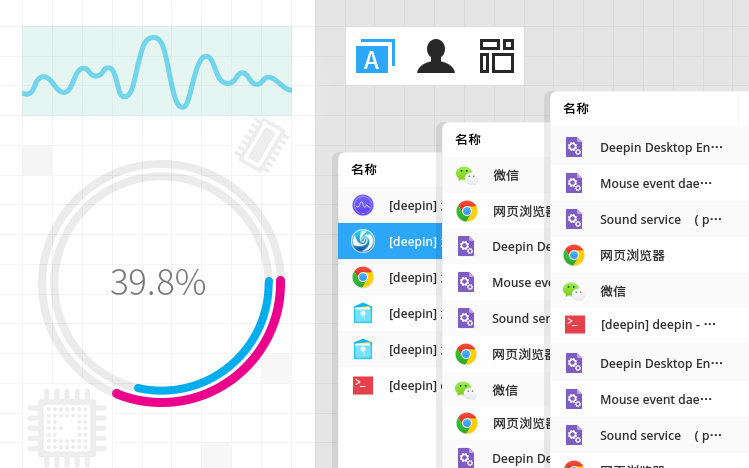
\includegraphics{images/deepin-system-monitor-3.jpg}
\caption{标签显示,快速定位}
\end{figure}

\textbf{列表展示,高效右键}

系统的进程采用列表方式展示,可以自定义处理器、内存、磁盘写入、磁盘读取、下载、上传、进程号是否显示,还可以根据列表排序显示;同时对进程还可以右键菜单快速操作。

\begin{figure}
\centering
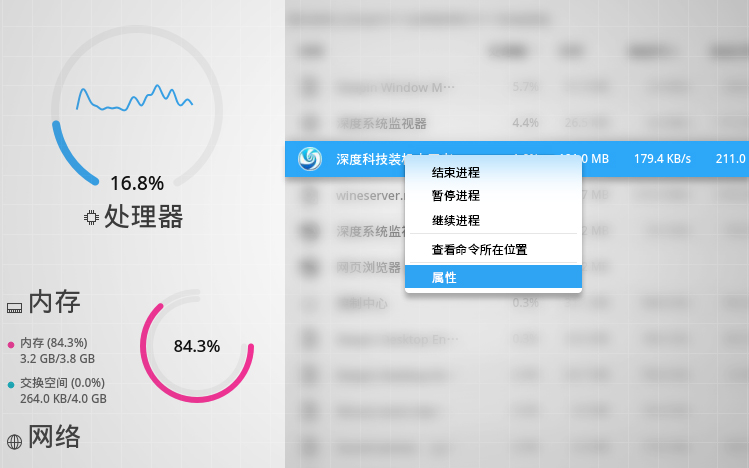
\includegraphics{images/deepin-system-monitor-4.jpg}
\caption{列表展示,高效右键}
\end{figure}

\textbf{捕捉窗口,即点即``杀''}

当在使用系统的过程,不知道进程的ID或者想直接结束某个应用进程,只需点击菜单中强制结束进程选项,自动采用红色透明遮框捕捉窗口,点击即可结束进程。

\begin{figure}
\centering
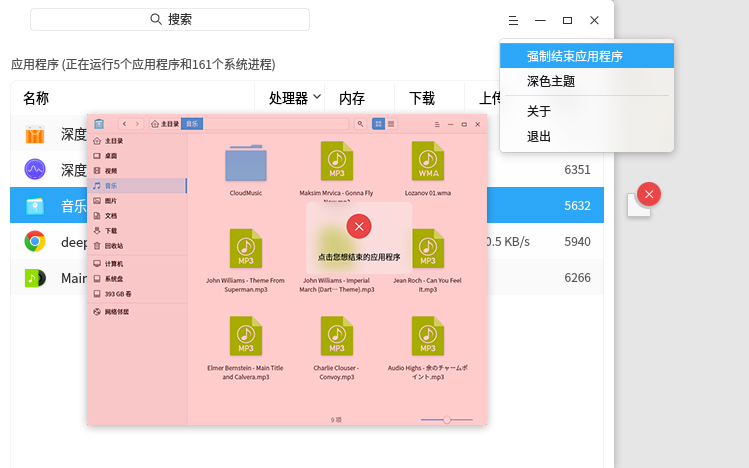
\includegraphics{images/deepin-system-monitor-5.jpg}
\caption{捕捉窗口,即点即``杀''}
\end{figure}

大家可以通过更新系统以获取深度系统监视器V1.0,或者直接在深度商店搜索下载。也可以采用命令行安装。

\begin{lstlisting}[language=bash]
$ sudo apt-get install deepin-system-monitor -y
\end{lstlisting}

\section{命令方式查看进程}

参考网页:

\begin{itemize}
\tightlist
\item
  \url{https://www.cnblogs.com/w10234/p/5642552.html}
\end{itemize}

要对进程进行监测和控制,首先必须要了解当前进程的情况,也就是需要查看当前进程,而\passthrough{\lstinline!ps!}命令(Process
Status)就是最基本同时也是非常强大的进程查看命令。使用该命令,可以确定有哪些进程正在运行和运行的状态、进程是否结束、进程有没有僵尸、哪些进程占用了过多的资源等等。

\passthrough{\lstinline!ps!}
为我们提供了进程的一次性的查看,它所提供的查看结果并不动态连续的;

如果想对进程时间监控并进行操作,应该用 \passthrough{\lstinline!top!}
工具。

如果直接用\passthrough{\lstinline!ps!}命令,会显示所有进程的状态,通常结合\passthrough{\lstinline!grep!}命令查看某进程的状态。\passthrough{\lstinline!grep!}命令已经在前面第\ref{chap:vim-find}章介绍过了。

\hypertarget{ps-}{%
\subsection{ps 命令基本用法}\label{ps-}}

按照\passthrough{\lstinline!man ps!}的说法,

\begin{quote}
This version of ps accepts several kinds of options:

\begin{enumerate}
\def\labelenumi{\arabic{enumi}.}
\tightlist
\item
  UNIX options, which may be grouped and must be preceded by a dash.
\item
  BSD options, which may be grouped and must not be used with a dash.
\item
  GNU long options, which are preceded by two dashes.
\end{enumerate}
\end{quote}

\passthrough{\lstinline!ps!}的选项支持三种方式,

\begin{enumerate}
\def\labelenumi{\arabic{enumi}.}
\tightlist
\item
  UNIX
  风格选项,可以组合且必须以短横线\passthrough{\lstinline!-!}开头,类似第\ref{chap:shell}章介绍的。
\item
  BSD 风格选项,可以组合且不可使用短横线。
\item
  GNU
  长风格选项,也即第\ref{chap:shell}章提到的双短横线\passthrough{\lstinline!--!}开头的选项。
\end{enumerate}

不同风格的选项可以混用,但是部分选项可能会相互冲突,比如\passthrough{\lstinline!ps aux!}跟\passthrough{\lstinline!ps -aux!}并不完全一样,详情请参考\passthrough{\lstinline!man ps!},这里不转载他们的内容了。下面介绍常用的几个例子。下面例子未经上机测试。特殊字符\passthrough{\lstinline!$!},\passthrough{\lstinline!\&!}在代码中由于是\passthrough{\lstinline!mathtype=true!},需要特别关注。

\begin{lstlisting}[language=bash]
$ # To see every process on the system using standard syntax:
$ ps -e
$ ps -ef
$ ps -eF
$ ps -ely
$ # To see every process on the system using BSD syntax:
$ ps ax
$ ps axu
$ # 查找包含php的进程
$ ps aux|grep php
$ # To print a process tree:
$ ps -ejH
$ ps axjf
$ # To get info about threads:
$ ps -eLf
$ ps axms
$ # To get security info:
$ ps -eo euser,ruser,suser,fuser,f,comm,label
$ ps axZ
$ ps -eM
$ # To see every process running as root (real \& effective ID) in user format:
$ ps -U root -u root u
$ # To see every process with a user-defined format:
$ ps -eo pid,tid,class,rtprio,ni,pri,psr,pcpu,stat,wchan:14,comm
$ ps axo stat,euid,ruid,tty,tpgid,sess,pgrp,ppid,pid,pcpu,comm
$ ps -Ao pid,tt,user,fname,tmout,f,wchan
$ # --sort=-rss是输出结果安装 rss从大到小排序,rss前正负号是否倒序。
$ ps -eo pid,user,group,gid,vsz,rss,comm --sort=-rss | less
$ # Print only the process IDs of syslogd:
$ ps -C syslogd -o pid=
$ # Print only the name of PID 42:
$ ps -q 42 -o comm=
\end{lstlisting}

对各个选项的简单解释如下,摘自:\url{https://www.cnblogs.com/w10234/p/5642552.html}

\begin{enumerate}
\def\labelenumi{\arabic{enumi}.}
\tightlist
\item
  \passthrough{\lstinline!ps a!}
  显示现行终端机下的所有程序,包括其他用户的程序。
\item
  \passthrough{\lstinline!ps -A!} 显示所有程序。
\item
  \passthrough{\lstinline!ps c!}
  列出程序时,显示每个程序真正的指令名称,而不包含路径,参数或常驻服务的标示。
\item
  \passthrough{\lstinline!ps -e!} 此参数的效果和指定``A''参数相同。
\item
  \passthrough{\lstinline!ps e!}
  列出程序时,显示每个程序所使用的环境变量。
\item
  \passthrough{\lstinline!ps f!}
  用ASCII字符显示树状结构,表达程序间的相互关系。
\item
  \passthrough{\lstinline!ps -H!} 显示树状结构,表示程序间的相互关系。
\item
  \passthrough{\lstinline!ps -N!}
  显示所有的程序,除了执行ps指令终端机下的程序之外。
\item
  \passthrough{\lstinline!ps s!} 采用程序信号的格式显示程序状况。
\item
  \passthrough{\lstinline!ps S!} 列出程序时,包括已中断的子程序资料。
\item
  \passthrough{\lstinline!ps -t<终端机编号>!} 指定终端机编号,并列出属于该终端机的程序的状况。
\item
  \passthrough{\lstinline!ps u!}  以用户为主的格式来显示程序状况。
\item
  \passthrough{\lstinline!ps x!}  显示所有程序,不以终端机来区分。
\end{enumerate}

\hypertarget{top-}{%
\subsection{top 命令基本用法}\label{top-}}

\passthrough{\lstinline!top!}动态实时的显示当前资源占用情况,如图\ref{fig:top-showing},并允许你对进程操作。如果你需要对所有的进程都能够生杀予夺,可能你需要\passthrough{\lstinline!root!}根权限。

\begin{figure}

{\centering 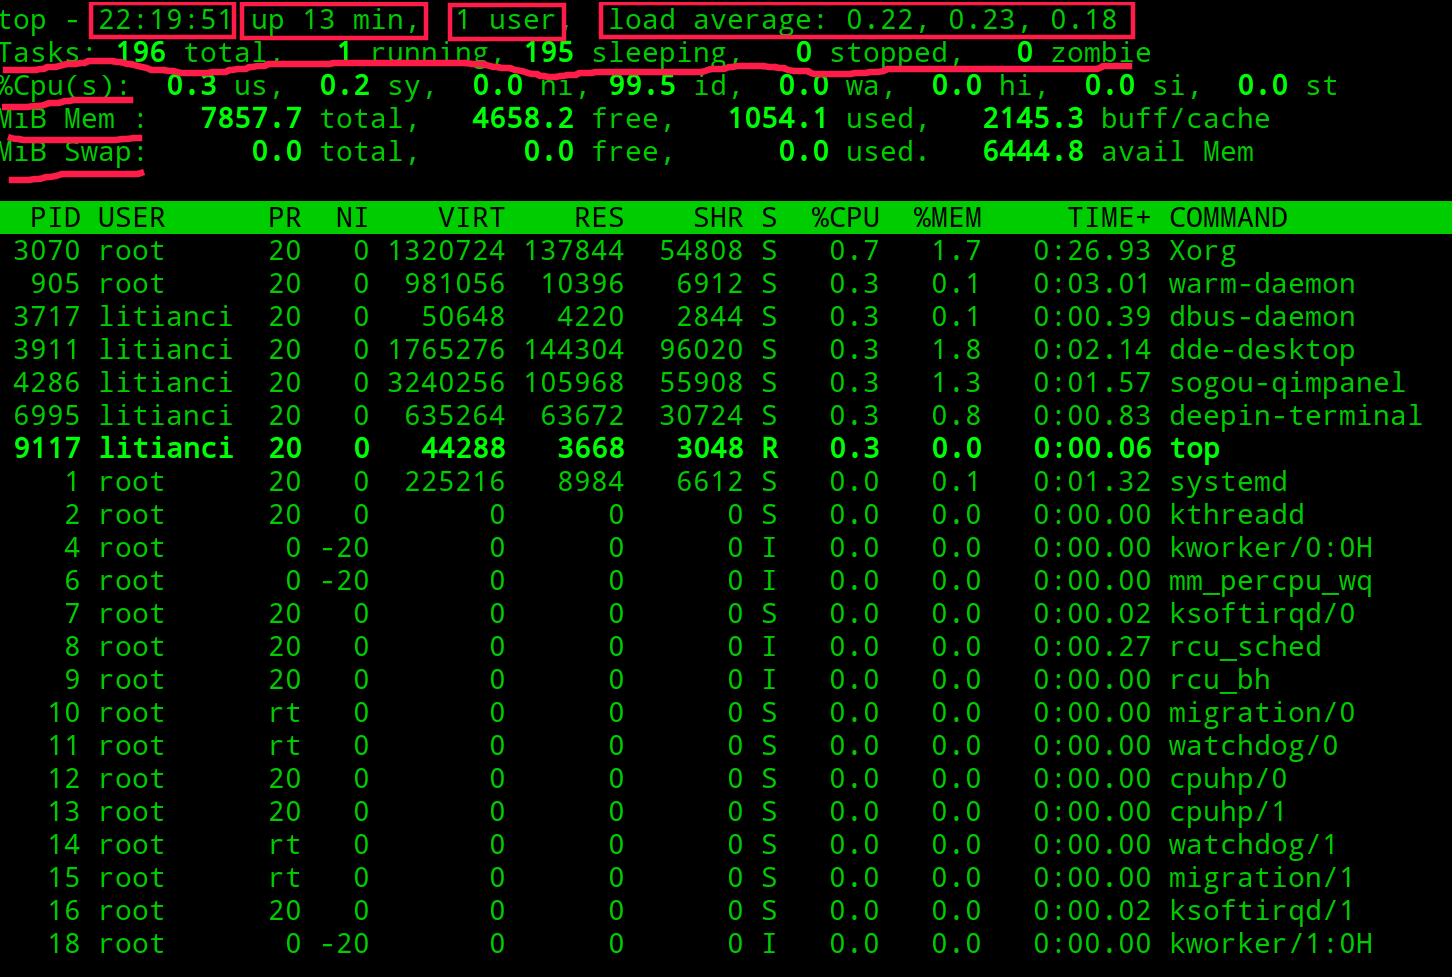
\includegraphics[width=1\linewidth]{images/top-showing} 

}

\caption[top显示界面]{top显示界面}\label{fig:top-showing}
\end{figure}

\textbf{解释}

\begin{enumerate}
\def\labelenumi{\arabic{enumi}.}
\tightlist
\item
  图中红色矩形框圈出的,表示当前时间\passthrough{\lstinline!22:19:51!},已经开机运行了多长时间\passthrough{\lstinline!13min!}(分钟),当前有\passthrough{\lstinline!1!}个用户,当前CPU负载。
\item
  图中手划线的分别表示进程统计信息\passthrough{\lstinline!Tasks!}、CPU及Ni等的信息\passthrough{\lstinline!\%Cpu(s)!}、内存占用情况(单位:MiB)\passthrough{\lstinline!MiB Mem!}、交换空间占用情况(单位:MiB)\passthrough{\lstinline!MiB Swap!}。对于MiB以及MB单位的区别,
\item
  按下\passthrough{\lstinline!h!}键,会弹出帮助信息。如图\ref{fig:top-help}所示。按下\passthrough{\lstinline!q!}或者\passthrough{\lstinline!esc!}键,返回到top命令界面。想看更多信息,可以\passthrough{\lstinline!man top!}或者必应百度一下。
\item
  按下\passthrough{\lstinline!M!}或\passthrough{\lstinline!P!},分别表示安装内存和CPU排序,数字\passthrough{\lstinline!1!}显示更多CPU,\passthrough{\lstinline!R!}表示正倒序切换。
\item
  按下\passthrough{\lstinline!u!},紧接着输入用户名回车,查看特定用户的进程。直接回车查看所有用户的进程。
\end{enumerate}

\begin{figure}

{\centering 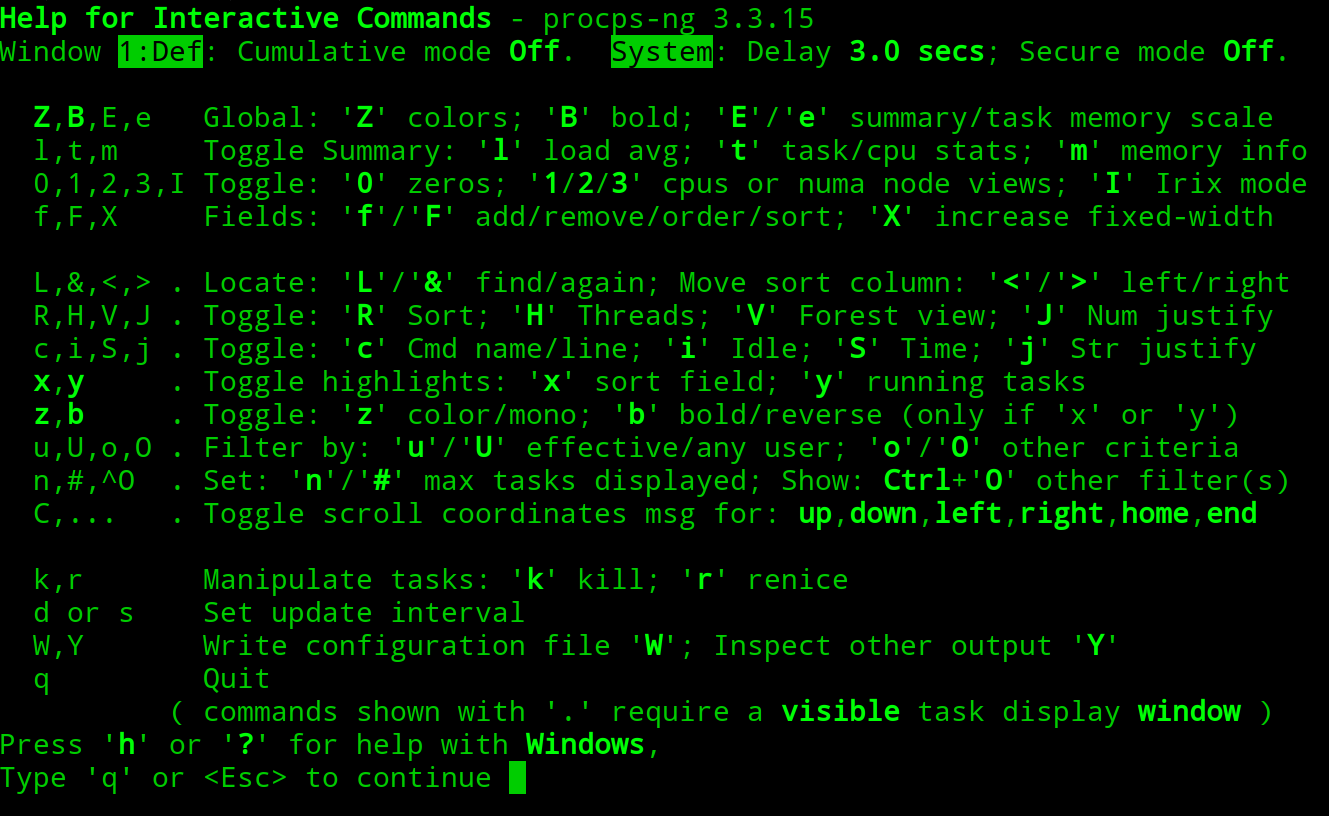
\includegraphics[width=1\linewidth]{images/top-help} 

}

\caption[top显示界面]{top显示界面}\label{fig:top-help}
\end{figure}

\BeginKnitrBlock{rmdtip}
众所周知,在计算机中是采用二进制,在电脑世界里,以2的次方数为``批量''处理Byte会方便一些,整齐一些。每1024Byte为1KB,每1024KB为1MB,每1024MB为1GB,每1024GB为1TB,而在国际单位制中TB、GB、MB、KB是``1000进制''的数,为此国际电工协会(IEC)拟定了``KiB''、``MiB''、``GiB''的二进制单位,专用来标示``1024进位''的数据大小;而硬盘厂商在计算容量方面是以每1000为一进制的,每1000字节为1KB,每1000KB为1MB,每1000MB为1GB,每1000GB为1TB

参考网页:
\url{https://blog.csdn.net/u012256258/article/details/52565500}
\EndKnitrBlock{rmdtip}

\textbf{调整进程}

通常我们使用\passthrough{\lstinline!top!}是电脑太卡了,想要看看哪些进程占用CPU或者内存过多。上面提到的按键\passthrough{\lstinline!M!}和\passthrough{\lstinline!P!}分别实现内存和CPU占用的排序,就非常有用,按\passthrough{\lstinline!R!}实现正倒序的切换。非常方便。接下来就需要对相关进程\cqh 动手\cqt 啦。

\begin{enumerate}
\def\labelenumi{\arabic{enumi}.}
\tightlist
\item
  降低权重,减小优先级。其实就是图\ref{fig:top-showing}中\passthrough{\lstinline!NI!}和\passthrough{\lstinline!PR!}那两栏。关于优先级的内容,详情见下文。在\passthrough{\lstinline!top!}下可以按\passthrough{\lstinline!r!}(表示renice调整好感值)键,接着输入你想提高好感(\passthrough{\lstinline!NI!})的进程PID,回车后再给他一个好感值。一般情况,对于普通用户只能提高进程的好感值,无权降低。好感值(\passthrough{\lstinline!NI!})越高,占用资源的权限就越低,详细内容后面再说。
\item
  干掉进程。当你知道某个进程PID,就可以按下\passthrough{\lstinline!k!}(表示kill干掉键,接着输入该PID,最后输入\passthrough{\lstinline!kill!}命令的选项值,比如\passthrough{\lstinline!15!}清屏或者绝情些用\passthrough{\lstinline!9!}。
\end{enumerate}

\section{进程的分类}

当你使用Putty远程连接服务器时,只有一个终端,你想后台跑一个程序,但是在此同时还想干其他事情,怎么办呢?那就用上后台程序啦。

在 Linux 中主要有两种类型的进程:

\begin{itemize}
\tightlist
\item
  前台进程(也称为交互式进程) -
  这些进程由终端会话初始化和控制。换句话说,需要有一个连接到系统中的用户来启动这样的进程;它们不是作为系统功能/服务的一部分自动启动。
\item
  后台进程(也称为非交互式/自动进程) -
  这些进程没有连接到终端;它们不需要任何用户输入。
\end{itemize}

什么是守护进程

这是后台进程的特殊类型,它们在系统启动时启动,并作为服务一直运行;它们不会死亡。它们自发地作为系统任务启动(作为服务运行)。但是,它们能被用户通过
init 进程控制。

\subsection{怎么生成后台进程呢?}

我感觉我的理解可能有误,比如我知道\passthrough{\lstinline!evince!}
PDF阅读器不锁定文件的修改,当你修改了PDF文件,可以从\passthrough{\lstinline!evince!}上直接看到变化。这对于编写本书反复编译太有帮助了。但是编译本书要运行\passthrough{\lstinline!make!}命令,我习惯只打开一个终端,我就可以让\passthrough{\lstinline!evince!}程序运行于后台。有这么几种方法,

\begin{itemize}
\tightlist
\item
  在命令行末尾加\passthrough{\lstinline!\&!}。
\item
  使用\passthrough{\lstinline!at!}命令(没有例子)。
\end{itemize}

\begin{lstlisting}[language=bash]
$ evince _book/deepin-bible.pdf &
[1] 19589
\end{lstlisting}

\textbf{解释}

\begin{enumerate}
\def\labelenumi{\arabic{enumi}.}
\tightlist
\item
  \passthrough{\lstinline![1]!}表示,后台进程序号。\passthrough{\lstinline!19589!}是进程号PID。
\end{enumerate}

如果想查看当前有多少后台进程。使用命令\passthrough{\lstinline!jobs!}

\begin{lstlisting}[language=bash]
$ jobs
[1]   运行中               evince _book/deepin-bible.pdf &
[2]-  已停止               man top
[3]+  已停止               vim ~/test.md
\end{lstlisting}

\textbf{解释}

\begin{enumerate}
\def\labelenumi{\arabic{enumi}.}
\tightlist
\item
  使用\passthrough{\lstinline!jobs!}会弹出当前正在运行的后台程序。还会显示他们的状态,比如运行中、已停止等。
\item
  \passthrough{\lstinline![3]+!},的\passthrough{\lstinline!+!},\passthrough{\lstinline!-!}号,表示最新和次新加入后台的进程。就是最后两个加入后台的进程。但是这个貌似不是非常准确。\passthrough{\lstinline!man top!}不是最新加入后台的进程,但是却被标注为最新加入的。好在这个不怎么影响,后面再去找资料核实。
\end{enumerate}

有时还需要把这些后台再拉回前台来,\passthrough{\lstinline!fg!}表示foreground的意思,就可以派上用场了。先看看\passthrough{\lstinline!fg!}的用法。貌似,不带\passthrough{\lstinline!\%!}也不影响结果。需要核实。

\begin{lstlisting}[language=bash]
$ fg % # 把最新的进程,也就是带`+`的进程放到前台。
$ fg %n # n表示`jobs`命令中[n]
$ fg %string # string 表示命令,比如 `vim`,前提是不混淆。
$ fg %?string # ?string表示 string 在任意位置。
$ fg %-- # 倒数第二个已停止的进程拉回前台。
\end{lstlisting}

当然,我试过\passthrough{\lstinline!fg n!}直接输入\passthrough{\lstinline!jobs!}命令出来的那些后台序号\passthrough{\lstinline![n]!},可以直接把他们拉回前台。另外还有\passthrough{\lstinline!bg!}命令,用于唤醒已停止的后台命令。

\hypertarget{killing-and-renicing}{%
\section{进程的终结与调整优先级(Killing and
Renicing)}\label{killing-and-renicing}}

有些进程太耗资源,我们需要关闭它,可以使用\passthrough{\lstinline!kill!}和\passthrough{\lstinline!killall!}命令,分别是通过进程号PID终结某个进程和通过进程名称终结某类进程。在终结进程的时候,还需要传递系统信号。具体用法可以通过\passthrough{\lstinline!man kill!}等查看。先来常用的几个例子吧,

\begin{lstlisting}[language=bash]
$ kill -l # 列出所有可用信号,见下面信号表
$ kill 999 # 使用默认系统信号杀死PID=999的进程
$ kill -15 999 # 默认系统信号也就是15号
$ kill -SIGKILL 999 # 默认系统信号常量为 SIGKILL,跟上面一致。
$ kill -9 999 # 对于顽固分子,电脑卡住的,往往用 -9 KILL 信号
$ killall -9 workrave # killall 使用的信号类似 kill,只不过用的是命令名称进行终结
\end{lstlisting}

参考网页:

\begin{itemize}
\tightlist
\item
  \url{http://www.cnblogs.com/taobataoma/archive/2007/08/30/875743.html}
\end{itemize}

\begin{longtable}[]{@{}ccl@{}}
\caption{信号对应的数值及意义}\tabularnewline
\toprule
\begin{minipage}[b]{0.10\columnwidth}\centering
\textbf{信号}\strut
\end{minipage} & \begin{minipage}[b]{0.12\columnwidth}\centering
\textbf{数值}\strut
\end{minipage} & \begin{minipage}[b]{0.70\columnwidth}\raggedright
\textbf{意义}\strut
\end{minipage}\tabularnewline
\midrule
\endfirsthead
\toprule
\begin{minipage}[b]{0.10\columnwidth}\centering
\textbf{信号}\strut
\end{minipage} & \begin{minipage}[b]{0.12\columnwidth}\centering
\textbf{数值}\strut
\end{minipage} & \begin{minipage}[b]{0.70\columnwidth}\raggedright
\textbf{意义}\strut
\end{minipage}\tabularnewline
\midrule
\endhead
\begin{minipage}[t]{0.10\columnwidth}\centering
SIGHUP\strut
\end{minipage} & \begin{minipage}[t]{0.12\columnwidth}\centering
1\strut
\end{minipage} & \begin{minipage}[t]{0.70\columnwidth}\raggedright
Hang-up detected on controlling terminal or death of controlling
process.\strut
\end{minipage}\tabularnewline
\begin{minipage}[t]{0.10\columnwidth}\centering
SIGINT\strut
\end{minipage} & \begin{minipage}[t]{0.12\columnwidth}\centering
2\strut
\end{minipage} & \begin{minipage}[t]{0.70\columnwidth}\raggedright
Interrupt from keyboard.\strut
\end{minipage}\tabularnewline
\begin{minipage}[t]{0.10\columnwidth}\centering
SIGQUIT\strut
\end{minipage} & \begin{minipage}[t]{0.12\columnwidth}\centering
3\strut
\end{minipage} & \begin{minipage}[t]{0.70\columnwidth}\raggedright
Quit from keyboard.\strut
\end{minipage}\tabularnewline
\begin{minipage}[t]{0.10\columnwidth}\centering
SIGABRT\strut
\end{minipage} & \begin{minipage}[t]{0.12\columnwidth}\centering
6\strut
\end{minipage} & \begin{minipage}[t]{0.70\columnwidth}\raggedright
Abort signal from abort(3).\strut
\end{minipage}\tabularnewline
\begin{minipage}[t]{0.10\columnwidth}\centering
SIGKILL\strut
\end{minipage} & \begin{minipage}[t]{0.12\columnwidth}\centering
9\strut
\end{minipage} & \begin{minipage}[t]{0.70\columnwidth}\raggedright
Kill signal.\strut
\end{minipage}\tabularnewline
\begin{minipage}[t]{0.10\columnwidth}\centering
SIGTERM\strut
\end{minipage} & \begin{minipage}[t]{0.12\columnwidth}\centering
15\strut
\end{minipage} & \begin{minipage}[t]{0.70\columnwidth}\raggedright
Termination signal.\strut
\end{minipage}\tabularnewline
\begin{minipage}[t]{0.10\columnwidth}\centering
SIGCONT\strut
\end{minipage} & \begin{minipage}[t]{0.12\columnwidth}\centering
19,18,25\strut
\end{minipage} & \begin{minipage}[t]{0.70\columnwidth}\raggedright
Continue if stopped.\strut
\end{minipage}\tabularnewline
\begin{minipage}[t]{0.10\columnwidth}\centering
SIGSTOP\strut
\end{minipage} & \begin{minipage}[t]{0.12\columnwidth}\centering
17,19,23\strut
\end{minipage} & \begin{minipage}[t]{0.70\columnwidth}\raggedright
Stop process.\strut
\end{minipage}\tabularnewline
\bottomrule
\end{longtable}

参考网页:

\begin{itemize}
\tightlist
\item
  \url{https://blog.csdn.net/longdel/article/details/7317511}
\end{itemize}

用\passthrough{\lstinline!top!}或者\passthrough{\lstinline!ps!}命令会输出\passthrough{\lstinline!PRI/PR!}、\passthrough{\lstinline!NI!}、\passthrough{\lstinline!\%ni/\%nice!}这三种指标值,这些到底是什么东西?先给出大概的解释如下:

\begin{itemize}
\tightlist
\item
  \passthrough{\lstinline!PRI!}
  :进程优先权,代表这个进程可被执行的优先级,其值越小,优先级就越高,越早被执行。
\item
  \passthrough{\lstinline!NI!}
  :进程\passthrough{\lstinline!nice!}值,代表这个进程的优先值。
\item
  \passthrough{\lstinline!\%nice!} :改变过优先级的进程占用CPU的百分比。
\end{itemize}

\passthrough{\lstinline!PRI!}是比较好理解的,即进程的优先级,或者通俗点说就是程序被CPU执行的先后顺序,此值越小进程的优先级别越高。那\passthrough{\lstinline!NI!}呢?就是我们所要说的\passthrough{\lstinline!nice!}值了,其表示进程可被执行的优先级的修正数值。如前面所说,\passthrough{\lstinline!PRI!}值越小越快被执行,那么加入\passthrough{\lstinline!nice!}值后,将会使得\passthrough{\lstinline!PRI!}变为:\passthrough{\lstinline!PRI(new)=PRI(old)+nice!}。由此看出,\passthrough{\lstinline!PRI!}是根据\passthrough{\lstinline!nice!}排序的,规则是\passthrough{\lstinline!nice!}越小\passthrough{\lstinline!PRI!}越前(小,优先权更大),即其优先级会变高,则其越快被执行。如果\passthrough{\lstinline!nice!}相同则进程\passthrough{\lstinline!uid!}是root的优先权更大。

在LINUX系统中,\passthrough{\lstinline!nice!}值的范围从\passthrough{\lstinline!-20!}到\passthrough{\lstinline!+19!}(不同系统的值范围是不一样的),正值表示低优先级,负值表示高优先级,值为零则表示不会调整该进程的优先级。具有最高优先级的程序,其\passthrough{\lstinline!nice!}值最低,所以在LINUX系统中,值\passthrough{\lstinline!-20!}使得一项任务变得非常重要;与之相反,如果任务的\passthrough{\lstinline!nice!}为\passthrough{\lstinline!+19!},则表示它是一个高尚的、无私的任务,允许所有其他任务比自己享有宝贵的CPU时间的更大使用份额,这也就是\passthrough{\lstinline!nice!}的名称的来意。

进程在创建时被赋予不同的优先级值,而如前面所说,\passthrough{\lstinline!nice!}的值是表示进程优先级值可被修正数据值,因此,每个进程都在其计划执行时被赋予一个\passthrough{\lstinline!nice!}值,这样系统就可以根据系统的资源以及具体进程的各类资源消耗情况,主动干预进程的优先级值。在通常情况下,子进程会继承父进程的\passthrough{\lstinline!nice!}值,比如在系统启动的过程中,\passthrough{\lstinline!init!}进程会被赋予\passthrough{\lstinline!0!},其他所有进程继承了这个\passthrough{\lstinline!nice!}值(因为其他进程都是\passthrough{\lstinline!init!}的子进程)。

对\passthrough{\lstinline!nice!}值一个形象比喻,假设在一个CPU轮转中,有2个\passthrough{\lstinline!runnable!}的进程A和B,如果他们的\passthrough{\lstinline!nice!}值都为0,假设内核会给他们每人分配\passthrough{\lstinline!1k!}个cpu时间片。但是假设进程A的为0,但是B的值为\passthrough{\lstinline!-10!},那么此时CPU可能分别给A和B分配\passthrough{\lstinline!1k!}和\passthrough{\lstinline!1.5k!}的时间片。故可以形象的理解为,\passthrough{\lstinline!nice!}的值影响了内核分配给进程的cpu时间片的多少,时间片越多的进程,其优先级越高,其优先级值(\passthrough{\lstinline!PRI!})越低。\passthrough{\lstinline!\%nice!},就是改变过优先级的进程的占用CPU的百分比,如上例中就是\passthrough{\lstinline!0.5k/2.5k=1/5=20\%!}。

由此可见,进程\passthrough{\lstinline!nice!}值和进程优先级不是一个概念,但是进程\passthrough{\lstinline!nice!}值会影响到进程的优先级变化。

进程的nice值是可以被修改的,修改命令分别是\passthrough{\lstinline!nice!}和\passthrough{\lstinline!renice!}。

\begin{enumerate}
\def\labelenumi{\arabic{enumi}.}
\tightlist
\item
  \passthrough{\lstinline!nice!}命令就是设置一个要执行command进程的\passthrough{\lstinline!nice!}值,其命令格式是
  \passthrough{\lstinline!nice –n adjustment command command\_option!}。如果这里不指定\passthrough{\lstinline!adjustment!},则默认为\passthrough{\lstinline!10!},非root用户,\passthrough{\lstinline!adjustment!}不可为负值。
\item
  \passthrough{\lstinline!renice!}命令就是设置一个已经在运行的进程的\passthrough{\lstinline!nice!}值,假设一运行进程本来\passthrough{\lstinline!nice!}值为\passthrough{\lstinline!0!},\passthrough{\lstinline!renice!}为\passthrough{\lstinline!3!}后,则这个运行进程的\passthrough{\lstinline!nice!}值就为\passthrough{\lstinline!3!}了。
\item
  如果用户设置的\passthrough{\lstinline!nice!}值超过了\passthrough{\lstinline!nice!}的边界值(LINUX为\passthrough{\lstinline!-20!}到\passthrough{\lstinline!+19!}),系统就取\passthrough{\lstinline!nice!}的边界值作为进程的\passthrough{\lstinline!nice!}值。
\item
  对非root用户,只能将其底下的进程的\passthrough{\lstinline!nice!}值变大而不能变小。若想变小,得要有相应的权限。
\end{enumerate}

\begin{lstlisting}[language=bash]
$ nice
0
$ nice -n 3 ls -l bashscript
-rwsrwxrwx 1 litianci litianci 119 11月 17 22:32 bashscript
$ nice -n -2 ls -l bashscript
nice: 无法设置优先级: 权限不够
-rwsrwxrwx 1 litianci litianci 119 11月 17 22:32 bashscript
$ sudo nice -n -2 ls -l bashscript
-rwsrwxrwx 1 litianci litianci 119 11月 17 22:32 bashscript
\end{lstlisting}

同样,\passthrough{\lstinline!renice!}与\passthrough{\lstinline!nice!}命令类似,但是需要输入已经运行的进程号PID。

\begin{lstlisting}[language=bash]
$ evince _book/deepin-bible.pdf & # 启动一个后台程序,显示了进程号
[1] 26159
$ renice -n 5 26159 # renice 该进程
26159 (process ID) old priority 0, new priority 5
\end{lstlisting}

\hypertarget{cgroups}{%
\section{\texorpdfstring{通过\texttt{cgroups}限制进程}{通过cgroups限制进程}}\label{cgroups}}

参考网页:

\begin{itemize}
\tightlist
\item
  \url{http://www.cnblogs.com/lisperl/archive/2012/04/17/2453838.html}
\end{itemize}

\hypertarget{cgroups}{%
\subsection{\texorpdfstring{\texttt{cgroups}是什么?}{cgroups是什么?}}\label{cgroups}}

\passthrough{\lstinline!cgroups!}是control
groups的缩写,是Linux内核提供的一种可以限制、记录、隔离进程组(process
groups)所使用的物理资源(如:cpu,memory,IO等等)的机制。最初由google的工程师提出,后来被整合进Linux内核。cgroups也是LXC为实现虚拟化所使用的资源管理手段,可以说没有cgroups就没有LXC。

\hypertarget{cgroups}{%
\subsection{\texorpdfstring{\texttt{cgroups}可以做什么?}{cgroups可以做什么?}}\label{cgroups}}

\passthrough{\lstinline!cgroups!}最初的目标是为资源管理提供的一个统一的框架,既整合现有的cpuset等子系统,也为未来开发新的子系统提供接口。现在的\passthrough{\lstinline!cgroups!}适用于多种应用场景,从单个进程的资源控制,到实现操作系统层次的虚拟化(OS
Level Virtualization)。

\passthrough{\lstinline!cgroups!}提供了以下功能:

\begin{enumerate}
\def\labelenumi{\arabic{enumi}.}
\tightlist
\item
  限制进程组可以使用的资源数量(Resource limiting
  )。比如:memory子系统可以为进程组设定一个memory使用上限,一旦进程组使用的内存达到限额再申请内存,就会出发OOM(out
  of memory)。
\item
  进程组的优先级控制(Prioritization
  )。比如:可以使用cpu子系统为某个进程组分配特定cpu share。
\item
  记录进程组使用的资源数量(Accounting
  )。比如:可以使用cpuacct子系统记录某个进程组使用的cpu时间
\item
  进程组隔离(Isolation)。比如:使用ns子系统可以使不同的进程组使用不同的namespace,以达到隔离的目的,不同的进程组有各自的进程、网络、文件系统挂载空间。
\item
  进程组控制(Control)。比如:使用freezer子系统可以将进程组挂起和恢复。
\end{enumerate}

\hypertarget{cgroups}{%
\subsection{\texorpdfstring{\texttt{cgroups}相关概念及其关系}{cgroups相关概念及其关系}}\label{cgroups}}

\textbf{相关概念:}

\begin{enumerate}
\def\labelenumi{\arabic{enumi}.}
\tightlist
\item
  任务(task)。在\passthrough{\lstinline!cgroups!}中,任务就是系统的一个进程。
\item
  控制族群(control
  group)。控制族群就是一组按照某种标准划分的进程。\passthrough{\lstinline!cgroups!}中的资源控制都是以控制族群为单位实现。一个进程可以加入到某个控制族群,也从一个进程组迁移到另一个控制族群。一个进程组的进程可以使用\passthrough{\lstinline!cgroups!}以控制族群为单位分配的资源,同时受到\passthrough{\lstinline!cgroups!}以控制族群为单位设定的限制。
\item
  层级(hierarchy)。控制族群可以组织成hierarchical的形式,即一颗控制族群树。控制族群树上的子节点控制族群是父节点控制族群的孩子,继承父控制族群的特定的属性。
\item
  子系统(subsytem)。一个子系统就是一个资源控制器,比如cpu子系统就是控制cpu时间分配的一个控制器。子系统必须附加(attach)到一个层级上才能起作用,一个子系统附加到某个层级以后,这个层级上的所有控制族群都受到这个子系统的控制。
\end{enumerate}

\textbf{相互关系:}

\begin{enumerate}
\def\labelenumi{\arabic{enumi}.}
\tightlist
\item
  每次在系统中创建新层级时,该系统中的所有任务都是那个层级的默认
  \passthrough{\lstinline!cgroup!}(我们称之为
  \passthrough{\lstinline!root cgroup!}
  ,此\passthrough{\lstinline!cgroup!}在创建层级时自动创建,后面在该层级中创建的\passthrough{\lstinline!cgroup!}都是此\passthrough{\lstinline!cgroup!}的后代)的初始成员。
\item
  一个子系统最多只能附加到一个层级。
\item
  一个层级可以附加多个子系统
\item
  一个任务可以是多个\passthrough{\lstinline!cgroup!}的成员,但是这些\passthrough{\lstinline!cgroup!}必须在不同的层级。
\item
  系统中的进程(任务)创建子进程(任务)时,该子任务自动成为其父进程所在
  \passthrough{\lstinline!cgroup!}
  的成员。然后可根据需要将该子任务移动到不同的
  \passthrough{\lstinline!cgroup!}
  中,但开始时它总是继承其父任务的\passthrough{\lstinline!cgroup!}。
\end{enumerate}

\hypertarget{cgroups}{%
\subsection{\texorpdfstring{\texttt{cgroups}子系统介绍}{cgroups子系统介绍}}\label{cgroups}}

\begin{itemize}
\tightlist
\item
  \passthrough{\lstinline!blkio!} --
  这个子系统为块设备设定输入/输出限制,比如物理设备(磁盘,固态硬盘,USB
  等等)。
\item
  \passthrough{\lstinline!cpu!} -- 这个子系统使用调度程序提供对 CPU 的
  \passthrough{\lstinline!cgroup!} 任务访问。
\item
  \passthrough{\lstinline!cpuacct!} -- 这个子系统自动生成
  \passthrough{\lstinline!cgroup!} 中任务所使用的 CPU 报告。
\item
  \passthrough{\lstinline!cpuset!} -- 这个子系统为
  \passthrough{\lstinline!cgroup!} 中的任务分配独立
  CPU(在多核系统)和内存节点。
\item
  \passthrough{\lstinline!devices!} -- 这个子系统可允许或者拒绝
  \passthrough{\lstinline!cgroup!} 中的任务访问设备。
\item
  \passthrough{\lstinline!freezer!} -- 这个子系统挂起或者恢复
  \passthrough{\lstinline!cgroup!} 中的任务。
\item
  \passthrough{\lstinline!memory!} -- 这个子系统设定
  \passthrough{\lstinline!cgroup!}
  中任务使用的内存限制,并自动生成由那些任务使用的内存资源报告。
\item
  \passthrough{\lstinline!net\_cls!} --
  这个子系统使用等级识别符(classid)标记网络数据包,可允许 Linux
  流量控制程序(tc)识别从具体 cgroup 中生成的数据包。
\item
  \passthrough{\lstinline!ns!} -- 名称空间子系统。
\end{itemize}

关于\passthrough{\lstinline!cgroups!}的更多介绍,请参考相关书籍。

\section{进程的状态}

参考网页:

\begin{itemize}
\tightlist
\item
  \url{https://blog.csdn.net/shenwansangz/article/details/51981459}
\end{itemize}

Linux是一个多用户,多任务的系统,可以同时运行多个用户的多个程序,就必然会产生很多的进程,而每个进程会有不同的状态。

\hypertarget{linuxr-task_running}{%
\subsection{Linux进程状态:R
(TASK\_RUNNING),可执行状态。}\label{linuxr-task_running}}

只有在该状态的进程才可能在CPU上运行。而同一时刻可能有多个进程处于可执行状态,这些进程的task\_struct结构(进程控制块)被放入对应CPU的可执行队列中(一个进程最多只能出现在一个CPU的可执行队列中)。进程调度器的任务就是从各个CPU的可执行队列中分别选择一个进程在该CPU上运行。

很多操作系统教科书将正在CPU上执行的进程定义为RUNNING状态、而将可执行但是尚未被调度执行的进程定义为READY状态,这两种状态在linux下统一为
TASK\_RUNNING状态。

\hypertarget{linuxs-task_interruptible}{%
\subsection{Linux进程状态:S
(TASK\_INTERRUPTIBLE),可中断的睡眠状态。}\label{linuxs-task_interruptible}}

处于这个状态的进程因为等待某某事件的发生(比如等待socket连接、等待信号量),而被挂起。这些进程的task\_struct结构被放入对应事件的等待队列中。当这些事件发生时(由外部中断触发、或由其他进程触发),对应的等待队列中的一个或多个进程将被唤醒。

通过\passthrough{\lstinline!ps!}命令我们会看到,一般情况下,进程列表中的绝大多数进程都处于TASK\_INTERRUPTIBLE状态(除非机器的负载很高)。毕竟CPU就这么一两个,进程动辄几十上百个,如果不是绝大多数进程都在睡眠,CPU又怎么响应得过来。

\hypertarget{linuxd-task_uninterruptible}{%
\subsection{Linux进程状态:D
(TASK\_UNINTERRUPTIBLE),不可中断的睡眠状态。}\label{linuxd-task_uninterruptible}}

与TASK\_INTERRUPTIBLE状态类似,进程处于睡眠状态,但是此刻进程是不可中断的。不可中断,指的并不是CPU不响应外部硬件的中断,而是指进程不响应异步信号。

绝大多数情况下,进程处在睡眠状态时,总是应该能够响应异步信号的。否则你将惊奇的发现,\passthrough{\lstinline!kill -9!}竟然杀不死一个正在睡眠的进程了!于是我们也很好理解,为什么\passthrough{\lstinline!ps!}命令看到的进程几乎不会出现TASK\_UNINTERRUPTIBLE状态,而总是TASK\_INTERRUPTIBLE状态。

而TASK\_UNINTERRUPTIBLE状态存在的意义就在于,内核的某些处理流程是不能被打断的。如果响应异步信号,程序的执行流程中就会被插入一段用于处理异步信号的流程(这个插入的流程可能只存在于内核态,也可能延伸到用户态),于是原有的流程就被中断了。(参见《linux内核异步中断浅析》)

在进程对某些硬件进行操作时(比如进程调用read系统调用对某个设备文件进行读操作,而read系统调用最终执行到对应设备驱动的代码,并与对应的物理设备进行交互),可能需要使用TASK\_UNINTERRUPTIBLE状态对进程进行保护,以避免进程与设备交互的过程被打断,造成设备陷入不可控的状态。这种情况下的TASK\_UNINTERRUPTIBLE状态总是非常短暂的,通过\passthrough{\lstinline!ps!}命令基本上不可能捕捉到。

\hypertarget{linuxt-task_stopped-or-task_traced}{%
\subsection{Linux进程状态:T (TASK\_STOPPED or
TASK\_TRACED),暂停状态或跟踪状态。}\label{linuxt-task_stopped-or-task_traced}}

向进程发送一个SIGSTOP信号,它就会因响应该信号而进入TASK\_STOPPED状态(除非该进程本身处于TASK\_UNINTERRUPTIBLE状态而不响应信号)。(SIGSTOP与SIGKILL信号一样,是非常强制的。不允许用户进程通过signal系列的系统调用重新设置对应的信号处理函数。)

向进程发送一个SIGCONT信号,可以让其从TASK\_STOPPED状态恢复到TASK\_RUNNING状态。

当进程正在被跟踪时,它处于TASK\_TRACED这个特殊的状态。``正在被跟踪''指的是进程暂停下来,等待跟踪它的进程对它进行操作。比如在gdb中对被跟踪的进程下一个断点,进程在断点处停下来的时候就处于TASK\_TRACED状态。而在其他时候,被跟踪的进程还是处于前面提到的那些状态。

对于进程本身来说,TASK\_STOPPED和TASK\_TRACED状态很类似,都是表示进程暂停下来。而TASK\_TRACED状态相当于在TASK\_STOPPED之上多了一层保护,处于TASK\_TRACED状态的进程不能响应SIGCONT信号而被唤醒。只能等到调试进程通过ptrace系统调用执行PTRACE\_CONT、PTRACE\_DETACH等操作(通过ptrace系统调用的参数指定操作),或调试进程退出,被调试的进程才能恢复TASK\_RUNNING状态。

\hypertarget{linuxz-task_dead---exit_zombie}{%
\subsection{Linux进程状态:Z (TASK\_DEAD -
EXIT\_ZOMBIE),退出状态,进程成为僵尸进程。}\label{linuxz-task_dead---exit_zombie}}

进程在退出的过程中,处于TASK\_DEAD状态。

在这个退出过程中,进程占有的所有资源将被回收,除了task\_struct结构(以及少数资源)以外。于是进程就只剩下task\_struct这么个空壳,故称为僵尸。

之所以保留task\_struct,是因为task\_struct里面保存了进程的退出码、以及一些统计信息。而其父进程很可能会关心这些信息。比如在shell中,\$?变量就保存了最后一个退出的前台进程的退出码,而这个退出码往往被作为if语句的判断条件。

当然,内核也可以将这些信息保存在别的地方,而将task\_struct结构释放掉,以节省一些空间。但是使用task\_struct结构更为方便,因为在内核中已经建立了从pid到task\_struct查找关系,还有进程间的父子关系。释放掉task\_struct,则需要建立一些新的数据结构,以便让父进程找到它的子进程的退出信息。

父进程可以通过wait系列的系统调用(如wait4、waitid)来等待某个或某些子进程的退出,并获取它的退出信息。然后wait系列的系统调用会顺便将子进程的尸体(task\_struct)也释放掉。

子进程在退出的过程中,内核会给其父进程发送一个信号,通知父进程来``收尸''。这个信号默认是SIGCHLD,但是在通过clone系统调用创建子进程时,可以设置这个信号。

只要父进程不退出,这个僵尸状态的子进程就一直存在。那么如果父进程退出了呢,谁又来给子进程``收尸''?
当进程退出的时候,会将它的所有子进程都托管给别的进程(使之成为别的进程的子进程)。托管给谁呢?可能是退出进程所在进程组的下一个进程(如果存在的话),或者是1号进程。所以每个进程、每时每刻都有父进程存在。除非它是1号进程。

1号进程,pid为1的进程,又称init进程。
linux系统启动后,第一个被创建的用户态进程就是init进程。它有两项使命:

\begin{enumerate}
\def\labelenumi{\arabic{enumi}.}
\tightlist
\item
  执行系统初始化脚本,创建一系列的进程(它们都是init进程的子孙);
\item
  在一个死循环中等待其子进程的退出事件,并调用waitid系统调用来完成``收尸''工作;
\end{enumerate}

init进程不会被暂停、也不会被杀死(这是由内核来保证的)。它在等待子进程退出的过程中处于TASK\_INTERRUPTIBLE状态,``收尸''过程中则处于TASK\_RUNNING状态。

\hypertarget{linuxx-task_dead---exit_dead}{%
\subsection{Linux进程状态:X (TASK\_DEAD -
EXIT\_DEAD),退出状态,进程即将被销毁。}\label{linuxx-task_dead---exit_dead}}

而进程在退出过程中也可能不会保留它的task\_struct。比如这个进程是多线程程序中被detach过的进程(进程?线程?参见《linux线程浅析》)。或者父进程通过设置SIGCHLD信号的handler为SIG\_IGN,显式的忽略了SIGCHLD信号。(这是posix的规定,尽管子进程的退出信号可以被设置为SIGCHLD以外的其他信号。)

此时,进程将被置于EXIT\_DEAD退出状态,这意味着接下来的代码立即就会将该进程彻底释放。所以EXIT\_DEAD状态是非常短暂的,几乎不可能通过ps命令捕捉到。

\subsection{进程的初始状态}

进程是通过fork系列的系统调用(fork、clone、vfork)来创建的,内核(或内核模块)也可以通过kernel\_thread函数创建内核进程。这些创建子进程的函数本质上都完成了相同的功能------将调用进程复制一份,得到子进程。(可以通过选项参数来决定各种资源是共享、还是私有。)

那么既然调用进程处于TASK\_RUNNING状态(否则,它若不是正在运行,又怎么进行调用?),则子进程默认也处于TASK\_RUNNING状态。

另外,在系统调用调用clone和内核函数kernel\_thread也接受CLONE\_STOPPED选项,从而将子进程的初始状态置为
TASK\_STOPPED。

\subsection{进程状态变迁}

进程自创建以后,状态可能发生一系列的变化,直到进程退出。而尽管进程状态有好几种,但是进程状态的变迁却只有两个方向------从TASK\_RUNNING状态变为非TASK\_RUNNING状态、或者从非TASK\_RUNNING状态变为TASK\_RUNNING状态。

也就是说,如果给一个TASK\_INTERRUPTIBLE状态的进程发送SIGKILL信号,这个进程将先被唤醒(进入TASK\_RUNNING状态),然后再响应SIGKILL信号而退出(变为TASK\_DEAD状态)。并不会从TASK\_INTERRUPTIBLE状态直接退出。

进程从非TASK\_RUNNING状态变为TASK\_RUNNING状态,是由别的进程(也可能是中断处理程序)执行唤醒操作来实现的。执行唤醒的进程设置被唤醒进程的状态为TASK\_RUNNING,然后将其task\_struct结构加入到某个CPU的可执行队列中。于是被唤醒的进程将有机会被调度执行。

而进程从TASK\_RUNNING状态变为非TASK\_RUNNING状态,则有两种途径:

\begin{enumerate}
\def\labelenumi{\arabic{enumi}.}
\tightlist
\item
  响应信号而进入TASK\_STOPED状态、或TASK\_DEAD状态;
\item
  执行系统调用主动进入TASK\_INTERRUPTIBLE状态(如nanosleep系统调用)、或TASK\_DEAD状态(如exit系统调用);或由于执行系统调用需要的资源得不到满足,而进入TASK\_INTERRUPTIBLE状态或TASK\_UNINTERRUPTIBLE状态(如select系统调用)。
\end{enumerate}

显然,这两种情况都只能发生在进程正在CPU上执行的情况下。

\hypertarget{-6}{%
\section{总结}\label{-6}}

本章简要介绍了进程概念,如何查看进程,并对进程进行操作控制。本书不会太详细的介绍某个命令,如果需要深入了解,请用\passthrough{\lstinline!man <command>!}查找,或者网上搜索相关资料。

\hypertarget{chap:simple-bash-scripts}{%
\chapter{简单bash脚本}\label{chap:simple-bash-scripts}}

通过阅读本章,你将会了解到以下几项内容。

\begin{itemize}
\tightlist
\item
  理解脚本的概念
\item
  bash进行判断和简单数学计算
\item
  bash 的流程结构
\item
  实现把UC视频缓存变为普通视频文件的脚本
\end{itemize}

\hypertarget{-shell-}{%
\section{何谓 shell 脚本}\label{-shell-}}

我认为就是最初的程序员一条条命令写得太累了,能不能把每行命令都放在一个文本文件里,让shell自己来读取呢,这样脚本就诞生了。囊括了命令、函数、变量等内容,实现一条命令完成众多工作的功能,可以复杂到启动系统,也可用简单到只有一条命令,类似
Windows 下的批处理文件。

\subsection{执行和调试}

由于 shell
脚本都是文本,可以用任意编辑器打开,可当做\passthrough{\lstinline!bash!}或\passthrough{\lstinline!zsh!}等
shell 的参数来逐行直接执行,比如我们新建一个文本文件,内写上,
\passthrough{\lstinline!uname -a!},保存为\passthrough{\lstinline!myscript!}。可以通过如下方式执行,
\lstset{mathescape=true}

\begin{lstlisting}[language=bash]
$\$$ echo 'uname -a' > myscript
$\$$ bash myscript 
Linux litianci-PC 4.15.0-29deepin-generic $\#$31 SMP Fri Jul 27 07:12:08 UTC 2018 x86_64 GNU/Linux
\end{lstlisting}

\lstset{mathescape=false}

\textbf{解释}

\begin{enumerate}
\def\labelenumi{\arabic{enumi}.}
\tightlist
\item
  第1行,创建\passthrough{\lstinline!myscript!}文件。
\item
  第2行,执行该脚本文件
\item
  第3行,输出结果。
\end{enumerate}

另外,也可用给脚本加上可执行权限,直接运行。通常在脚本第一行\passthrough{\lstinline"#!/bin/bash"}告诉
shell 使用 \passthrough{\lstinline!/bin/bash!}
执行该脚本。对于使用\passthrough{\lstinline!Python!}或者\passthrough{\lstinline!R!}语言等执行的脚本,相应的把\passthrough{\lstinline!/bin/bash!}换成相应的脚本解释器\passthrough{\lstinline!Python!}或者\passthrough{\lstinline!RScript!}等。

在 shell 脚本中,使用 \passthrough{\lstinline!#!} 表示单行注释,也就是从
\passthrough{\lstinline!#!}
到行尾的内容为注释内容。当然,有些\passthrough{\lstinline!#!}属于字符串的内容或者其他语法格式,不表示单行注释。如果你使用\passthrough{\lstinline!vim!}等编辑器打开脚本的时候,会发现注释的颜色是跟其他部分不一样的。通常在脚本第二行开始该脚本的功能注释,也可以添加作者、编辑信息等,然后另起一行注释该脚本的名称。空一行,开始脚本正文内容。如下面所示,

\begin{lstlisting}[language=bash]
#!/bin/bash
# 本脚本实现 UC 浏览器视频缓存内容转换为一个完整的 MP4 文件
# ucvideo

if [! -e $2]
    echo "请按照如下格式调用该脚本"
fi
\end{lstlisting}

写完脚本,保存后,一般使用\passthrough{\lstinline!chmod u+x ucvideo!}的方式,给该脚本添加可执行权限。这样,可以像普通命令那样直接调用该脚本了。

\begin{lstlisting}[language=bash]
$ ./ucvideo
\end{lstlisting}

当然,跟其他程序类似,脚本不可避免的要调试纠错,下面几种方法可能有用,

\begin{itemize}
\tightlist
\item
  注释掉某些内容,方法就是在行首加\passthrough{\lstinline!#!};
\item
  使用
  \passthrough{\lstinline!echo!}输出相关参数信息或者其他需要显示的内容。
\item
  使用\passthrough{\lstinline!bash -x myscript!},会输出每行命令及执行结果,对于循环或者分支判断语句,可以告诉你具体执行了那些内容。
\end{itemize}

当然,最主要的还是要做到代码整洁,及时给自己的代码注释,避免后面自己都忘记咋回事了。

\hypertarget{shell-}{%
\subsection{shell 变量}\label{shell-}}

为了存储一些输出结果,或者一些参数等,需要用到变量存储,方便脚本书写。对于内容偏大的临时结果,也可用使用文件存储。通常采用如下方式,

\begin{lstlisting}[language=bash]
NAME=value
\end{lstlisting}

变量名\passthrough{\lstinline!NAME!}类似C语言的变量名规则,只可数字字母下划线,数字不可开头,区分大小写,中文不能出现在变量名中。对于变量值\passthrough{\lstinline!value!}则没有太多要求。通常是字符串、数字等,可以包含中文。比如,

\begin{lstlisting}[language=bash]
HOME="中国"
e=2.7
\end{lstlisting}

对于命令的输出结果,通常采用\passthrough{\lstinline!$(command)!}和\passthrough{\lstinline!`command`!}的方式实现。比如,

\begin{lstlisting}[language=bash]
MACHINE=`uname -n`
TODAY=$(date)
\end{lstlisting}

如果想获取变量的数值,可以使用\passthrough{\lstinline!$NAME!}的方法。

\begin{lstlisting}[language=bash]
echo $MACHINE
\end{lstlisting}

第\ref{chap:shell}章,简要介绍了\passthrough{\lstinline!$!},\passthrough{\lstinline!`!},\passthrough{\lstinline!*!},\passthrough{\lstinline"!"}等特殊字符。在脚本中有时需要他们的特殊功能,有时候需要他们保持原样,该怎么做呢,通常使用双引号\passthrough{\lstinline!""!},单引号\passthrough{\lstinline!''!},以及反斜杠\passthrough{\lstinline!\\!},看下面例子。

\begin{lstlisting}[language=bash]
$ echo $HOME
/home/litianci
$ echo "$HOME , today is `date`"
/home/litianci,today is 2018年 11月 16日 星期五 21:25:46 CST
$ echo '$HOME , today is `date`'
$HOME , today is `date`
$ echo \$HOME \`date\`
$HOME `date`
\end{lstlisting}

特殊字符可以使用\passthrough{\lstinline!\\!}转义为本来样子,直接输出即可。如果作为字符串,使用单引号\passthrough{\lstinline!'!}则保持原样不变,使用双引号\passthrough{\lstinline!"!}则实现转义。这在其他语言中也有类似做法。

\subsection{特殊变量}

作为脚本,作为命令来用时,不可避免的要传入参数,在脚本中,通常使用\passthrough{\lstinline!$0,$1,...,$n!}的方式来获取这些参数值。其中
\passthrough{\lstinline!$0!},表示本脚本;\passthrough{\lstinline!$n!},表示第\passthrough{\lstinline!n!}个输入参数。不管是\passthrough{\lstinline!bash myscript!}还是\passthrough{\lstinline!./myscript!}方式执行脚本,上述\passthrough{\lstinline!$n!}(\(n!=0\))都是一样的。另外\passthrough{\lstinline!$#!}表示共有多少个参数,\passthrough{\lstinline!$@!}保存着正行的输入。\passthrough{\lstinline!$?!}显示上一个命令的返回状态,一般返回\passthrough{\lstinline!0!}表示正常,其他数值表示异常或错误。看下面例子,脚本\passthrough{\lstinline!myscript!}的内容为。
\lstset{mathescape=true}

\begin{lstlisting}[language=bash]
#!/bin/bash
# 测试这些特使变量
# myscript

echo "第一个参数为: $\$$1, 第二个参数为 $\$$2."
echo "共有 $\$$$\#$ 个参数"
echo "这些参数是 $\$$@"
echo "该脚本名称为: $\$$0."
\end{lstlisting}

\lstset{mathescape=false}

分别执行\passthrough{\lstinline!bash myscript first second!}和\passthrough{\lstinline!./myscript first second!},结果如下,

\begin{lstlisting}[language=bash]
$ bash myscript first second
第一个参数为: first, 第二个参数为 second.
共有 2 个参数
这些参数是 first second
该脚本名称为: myscript.
$ chmod u+x myscript # 设置文件执行属性
$ ./myscript first second
第一个参数为: first, 第二个参数为 second.
共有 2 个参数
这些参数是 first second
该脚本名称为: ./myscript.
$ echo $?
0
\end{lstlisting}

\subsection{执行时输入参数}

\passthrough{\lstinline!$n!}(\passthrough{\lstinline!n>0!})一般都是执行前输入的参数,有时候还需要在执行中跟用户交互,那就用到\passthrough{\lstinline!read!}命令了。新建脚本\passthrough{\lstinline!readscript!}内容如下,

\begin{lstlisting}[language=bash]
#!/bin/bash
# 测试交互信息
# readscript

read -p "你叫啥名字,几岁啦?(两个答案请用空格隔开)" name age
echo "我知道啦,你叫 $name, $age 岁了。"
\end{lstlisting}

执行该脚本,

\begin{lstlisting}[language=bash]
$ bash readscript 
你叫啥名字,几岁啦?(两个答案请用空格隔开)深度易经 3
我知道啦,你叫 深度易经, 3 岁了。
\end{lstlisting}

关于\passthrough{\lstinline!read!}命令的更多内容,比如输入密码,或者其他信息,请\passthrough{\lstinline!read --help!}查看。

\subsection{其他需求的参数}

有些脚本,输入的参数可能有默认值,使用\passthrough{\lstinline!var1=$\{var2:-defaultvalue\}!}的方式,意思是变量\passthrough{\lstinline!var2!}如果存在赋值给\passthrough{\lstinline!var1!},否则,把\passthrough{\lstinline!defaultvalue!}赋值给\passthrough{\lstinline!var1!}。

\begin{lstlisting}[language=bash]
$ Birthday="2018-11-11"
$ Birthday=${Birthday:-`date`}
$ echo $Birthday
2018-11-11
$ Birthday=${DefaultDate:-`date`}
$ echo $Birthday
echo $Birthday 
2018年 11月 19日 星期一 21:48:35 CST
$ Name=${Name:-'尚未设置'}
$ echo $Name
尚未设置
\end{lstlisting}

有时,我们需要对参数再处理,比如对于路径的不同取舍,对某些合并参数等的提取,可能使用其他正则表达式截取部分字符串更合适,不过
Shell 还是提供了一些简单的截取功能。

\begin{itemize}
\tightlist
\item
  \passthrough{\lstinline!$\{var#pattern\}!}:从头删除满足匹配模式\passthrough{\lstinline!pattern!}的最短子字符串。
\item
  \passthrough{\lstinline!$\{var##pattern\}!}:从头删除满足匹配模式\passthrough{\lstinline!pattern!}的最长子字符串。
\item
  \passthrough{\lstinline!$\{var\%pattern\}!}:从尾删除满足匹配模式\passthrough{\lstinline!pattern!}的最短子字符串。
\item
  \passthrough{\lstinline!$\{var\%\%pattern\}!}:从尾删除满足匹配模式\passthrough{\lstinline!pattern!}的最长子字符串。
\end{itemize}

\lstset{mathescape=true}

\begin{lstlisting}[language=bash]
$\$$ readme=/home/litianci/deepin-bible/Readme.md
$\$$ file=$\$${readme$\#$$\#$*/}
$\$$ echo $\$$file 
Readme.md
$\$$ dir=$\$${readme%/*}
$\$$ echo $\$$dir
/home/litianci/deepin-bible
$\$$ stringchar="--folder=ucvideo"
$\$$ option=$\$${stringchar%=*}
$\$$ echo $\$$option
--folder
$\$$ value=$\$${stringchar$\#$*=}
$\$$ echo $\$$value
ucvideo
\end{lstlisting}

\lstset{mathescape=false}

\subsection{简单计算}

bash
认为所有的输入都是字符串或者文本,如果你想让bash理解为数字,貌似只可以整数,就得声明,比如使用\passthrough{\lstinline!let!},\passthrough{\lstinline!expr!},\passthrough{\lstinline!bc!}等方式。

\begin{lstlisting}[language=bash]
Total=1024
let div=$Total/8 # let表达式中间不可以有空格,所有参数必须为整数
div=`echo "$Total / 8" | bc` # bc对空格不敏感,可以有小数,但是结果还是取整
div=`echo "$Total       /       9.8      " | bc`
div=`echo "$Total/9.8" | bc`
div=`expr $Total / 8` # expr 必须有空格,所有参数必须为整数
echo $RANDOM # random 生成随机数
\end{lstlisting}

同时使用\passthrough{\lstinline!((statement))!}也可用实现简单的数学语句,

\begin{lstlisting}[language=bash]
i=0
((i++))
echo $i
echo $((i++))
echo $((++i))
((i=i+10))
echo $i
\end{lstlisting}

其中\passthrough{\lstinline!i++!}跟\passthrough{\lstinline!++i!}实现\passthrough{\lstinline!i!}数值加一,这两者区别类似C语言的规定,\passthrough{\lstinline!i++!}是先使用后递增一,\passthrough{\lstinline!++i!}是先递增一再使用。

\hypertarget{shell-}{%
\section{shell 脚本的三大结构}\label{shell-}}

学过编程语言的,应当多多少少都知道结构化编程语言的三大结构:\href{https://en.wikipedia.org/wiki/Structured_programming}{顺序、分支和循环}。shell
脚本支持这三种结构的。顺序执行就是逐行执行的命令,这里略过,下面介绍分支结构的语法。

\subsection{分支结构的语法}

\hypertarget{if-then-}{%
\subsubsection{\texorpdfstring{\texttt{if\ then}
语句}{if then 语句}}\label{if-then-}}

语法结构如下,

\begin{lstlisting}[language=bash]
if [ condition1 ] ; then
    statement1
elif [ condition2 ] ; then
    statement2
else
    statement3
fi
\end{lstlisting}

\textbf{解释}

\begin{enumerate}
\def\labelenumi{\arabic{enumi}.}
\tightlist
\item
  \passthrough{\lstinline![ condition1 ]!}这里是测试语句,用于测试条件是否满足,满足则执行\passthrough{\lstinline!statement1!}语句。
\item
  \passthrough{\lstinline!elif!}
  是\passthrough{\lstinline!else if!}的意思,用于多个测试条件。
\item
  其中\passthrough{\lstinline!elif!}和\passthrough{\lstinline!else!}部分可以不要。
\item
  \passthrough{\lstinline!fi!}其实是\passthrough{\lstinline!if!}的倒序写法。后面的\passthrough{\lstinline!case!}的结尾语句\passthrough{\lstinline!esac!}是同样的处理方式。
\end{enumerate}

\begin{lstlisting}[language=bash]
touch emptyfile
if [ ! -s dsffyfile ] ; then
    echo "emptyfile 是一个空文件"
fi
\end{lstlisting}

\textbf{解释}

\begin{enumerate}
\def\labelenumi{\arabic{enumi}.}
\tightlist
\item
  \passthrough{\lstinline"[ ! -s emptyfile ]"}中\passthrough{\lstinline!-s!}判断一个文件存在且非空是为真,\passthrough{\lstinline"!"}是逻辑运算取反的意思。
\item
  测试条件,需要注意\passthrough{\lstinline![]!}以及各个选项、运算符、参数均用空格\passthrough{\lstinline!!}隔开。
\item
  关于测试条件的更多信息,可以使用\passthrough{\lstinline!help test!}命令查看。
\end{enumerate}

\begin{longtable}[]{@{}cl@{}}
\caption{常见测试语句含义(\passthrough{\lstinline!help test!}截取)}\tabularnewline
\toprule
\begin{minipage}[b]{0.20\columnwidth}\centering
\textbf{测试语句}\strut
\end{minipage} & \begin{minipage}[b]{0.74\columnwidth}\raggedright
\textbf{解释}\strut
\end{minipage}\tabularnewline
\midrule
\endfirsthead
\toprule
\begin{minipage}[b]{0.20\columnwidth}\centering
\textbf{测试语句}\strut
\end{minipage} & \begin{minipage}[b]{0.74\columnwidth}\raggedright
\textbf{解释}\strut
\end{minipage}\tabularnewline
\midrule
\endhead
\begin{minipage}[t]{0.20\columnwidth}\centering
\passthrough{\lstinline!-a FILE!}\strut
\end{minipage} & \begin{minipage}[t]{0.74\columnwidth}\raggedright
True if file exists.\strut
\end{minipage}\tabularnewline
\begin{minipage}[t]{0.20\columnwidth}\centering
\passthrough{\lstinline!-b FILE!}\strut
\end{minipage} & \begin{minipage}[t]{0.74\columnwidth}\raggedright
True if file is block special.\strut
\end{minipage}\tabularnewline
\begin{minipage}[t]{0.20\columnwidth}\centering
\passthrough{\lstinline!-c FILE!}\strut
\end{minipage} & \begin{minipage}[t]{0.74\columnwidth}\raggedright
True if file is character special.\strut
\end{minipage}\tabularnewline
\begin{minipage}[t]{0.20\columnwidth}\centering
\passthrough{\lstinline!-d FILE!}\strut
\end{minipage} & \begin{minipage}[t]{0.74\columnwidth}\raggedright
True if file is a directory.\strut
\end{minipage}\tabularnewline
\begin{minipage}[t]{0.20\columnwidth}\centering
\passthrough{\lstinline!-e FILE!}\strut
\end{minipage} & \begin{minipage}[t]{0.74\columnwidth}\raggedright
True if file exists.\strut
\end{minipage}\tabularnewline
\begin{minipage}[t]{0.20\columnwidth}\centering
\passthrough{\lstinline!-f FILE!}\strut
\end{minipage} & \begin{minipage}[t]{0.74\columnwidth}\raggedright
True if file exists and is a regular file.\strut
\end{minipage}\tabularnewline
\begin{minipage}[t]{0.20\columnwidth}\centering
\passthrough{\lstinline!-g FILE!}\strut
\end{minipage} & \begin{minipage}[t]{0.74\columnwidth}\raggedright
True if file is set-group-id.\strut
\end{minipage}\tabularnewline
\begin{minipage}[t]{0.20\columnwidth}\centering
\passthrough{\lstinline!-h FILE!}\strut
\end{minipage} & \begin{minipage}[t]{0.74\columnwidth}\raggedright
True if file is a symbolic link.\strut
\end{minipage}\tabularnewline
\begin{minipage}[t]{0.20\columnwidth}\centering
\passthrough{\lstinline!-L FILE!}\strut
\end{minipage} & \begin{minipage}[t]{0.74\columnwidth}\raggedright
True if file is a symbolic link.\strut
\end{minipage}\tabularnewline
\begin{minipage}[t]{0.20\columnwidth}\centering
\passthrough{\lstinline!-k FILE!}\strut
\end{minipage} & \begin{minipage}[t]{0.74\columnwidth}\raggedright
True if file has its `sticky' bit set.\strut
\end{minipage}\tabularnewline
\begin{minipage}[t]{0.20\columnwidth}\centering
\passthrough{\lstinline!-p FILE!}\strut
\end{minipage} & \begin{minipage}[t]{0.74\columnwidth}\raggedright
True if file is a named pipe.\strut
\end{minipage}\tabularnewline
\begin{minipage}[t]{0.20\columnwidth}\centering
\passthrough{\lstinline!-r FILE!}\strut
\end{minipage} & \begin{minipage}[t]{0.74\columnwidth}\raggedright
True if file is readable by you.\strut
\end{minipage}\tabularnewline
\begin{minipage}[t]{0.20\columnwidth}\centering
\passthrough{\lstinline!-s FILE!}\strut
\end{minipage} & \begin{minipage}[t]{0.74\columnwidth}\raggedright
True if file exists and is not empty.\strut
\end{minipage}\tabularnewline
\begin{minipage}[t]{0.20\columnwidth}\centering
\passthrough{\lstinline!-S FILE!}\strut
\end{minipage} & \begin{minipage}[t]{0.74\columnwidth}\raggedright
True if file is a socket.\strut
\end{minipage}\tabularnewline
\begin{minipage}[t]{0.20\columnwidth}\centering
\passthrough{\lstinline!-t FD!}\strut
\end{minipage} & \begin{minipage}[t]{0.74\columnwidth}\raggedright
True if FD is opened on a terminal.\strut
\end{minipage}\tabularnewline
\begin{minipage}[t]{0.20\columnwidth}\centering
\passthrough{\lstinline!-u FILE!}\strut
\end{minipage} & \begin{minipage}[t]{0.74\columnwidth}\raggedright
True if the file is set-user-id.\strut
\end{minipage}\tabularnewline
\begin{minipage}[t]{0.20\columnwidth}\centering
\passthrough{\lstinline!-w FILE!}\strut
\end{minipage} & \begin{minipage}[t]{0.74\columnwidth}\raggedright
True if the file is writable by you.\strut
\end{minipage}\tabularnewline
\begin{minipage}[t]{0.20\columnwidth}\centering
\passthrough{\lstinline!-x FILE!}\strut
\end{minipage} & \begin{minipage}[t]{0.74\columnwidth}\raggedright
True if the file is executable by you.\strut
\end{minipage}\tabularnewline
\begin{minipage}[t]{0.20\columnwidth}\centering
\passthrough{\lstinline!-O FILE!}\strut
\end{minipage} & \begin{minipage}[t]{0.74\columnwidth}\raggedright
True if the file is effectively owned by you.\strut
\end{minipage}\tabularnewline
\begin{minipage}[t]{0.20\columnwidth}\centering
\passthrough{\lstinline!-G FILE!}\strut
\end{minipage} & \begin{minipage}[t]{0.74\columnwidth}\raggedright
True if the file is effectively owned by your group.\strut
\end{minipage}\tabularnewline
\begin{minipage}[t]{0.20\columnwidth}\centering
\passthrough{\lstinline!-N FILE!}\strut
\end{minipage} & \begin{minipage}[t]{0.74\columnwidth}\raggedright
True if the file has been modified since it was last read.\strut
\end{minipage}\tabularnewline
\begin{minipage}[t]{0.20\columnwidth}\centering
\passthrough{\lstinline!FILE1 -nt FILE2!}\strut
\end{minipage} & \begin{minipage}[t]{0.74\columnwidth}\raggedright
True if file1 is newer than file2 (according to modification
date).\strut
\end{minipage}\tabularnewline
\begin{minipage}[t]{0.20\columnwidth}\centering
\passthrough{\lstinline!FILE1 -ot FILE2!}\strut
\end{minipage} & \begin{minipage}[t]{0.74\columnwidth}\raggedright
True if file1 is older than file2.\strut
\end{minipage}\tabularnewline
\begin{minipage}[t]{0.20\columnwidth}\centering
\passthrough{\lstinline!FILE1 -ef FILE2!}\strut
\end{minipage} & \begin{minipage}[t]{0.74\columnwidth}\raggedright
True if file1 is a hard link to file2.\strut
\end{minipage}\tabularnewline
\begin{minipage}[t]{0.20\columnwidth}\centering
\passthrough{\lstinline!-z STRING!}\strut
\end{minipage} & \begin{minipage}[t]{0.74\columnwidth}\raggedright
True if string is empty.\strut
\end{minipage}\tabularnewline
\begin{minipage}[t]{0.20\columnwidth}\centering
\passthrough{\lstinline!-n STRING!}\strut
\end{minipage} & \begin{minipage}[t]{0.74\columnwidth}\raggedright
True if string is not empty.\strut
\end{minipage}\tabularnewline
\begin{minipage}[t]{0.20\columnwidth}\centering
\passthrough{\lstinline!STRING!}\strut
\end{minipage} & \begin{minipage}[t]{0.74\columnwidth}\raggedright
True if string is not empty.\strut
\end{minipage}\tabularnewline
\begin{minipage}[t]{0.20\columnwidth}\centering
\passthrough{\lstinline!STRING1 = STRING2!}\strut
\end{minipage} & \begin{minipage}[t]{0.74\columnwidth}\raggedright
True if the strings are equal.\strut
\end{minipage}\tabularnewline
\begin{minipage}[t]{0.20\columnwidth}\centering
\passthrough{\lstinline"STRING1 != STRING2"}\strut
\end{minipage} & \begin{minipage}[t]{0.74\columnwidth}\raggedright
True if the strings are not equal.\strut
\end{minipage}\tabularnewline
\begin{minipage}[t]{0.20\columnwidth}\centering
\passthrough{\lstinline!STRING1 < STRING2!}\strut
\end{minipage} & \begin{minipage}[t]{0.74\columnwidth}\raggedright
True if STRING1 sorts before STRING2 lexicographically.\strut
\end{minipage}\tabularnewline
\begin{minipage}[t]{0.20\columnwidth}\centering
\passthrough{\lstinline!STRING1 > STRING2!}\strut
\end{minipage} & \begin{minipage}[t]{0.74\columnwidth}\raggedright
True if STRING1 sorts after STRING2 lexicographically.\strut
\end{minipage}\tabularnewline
\begin{minipage}[t]{0.20\columnwidth}\centering
\passthrough{\lstinline!-o OPTION!}\strut
\end{minipage} & \begin{minipage}[t]{0.74\columnwidth}\raggedright
True if the shell option OPTION is enabled.\strut
\end{minipage}\tabularnewline
\begin{minipage}[t]{0.20\columnwidth}\centering
\passthrough{\lstinline!-v VAR!}\strut
\end{minipage} & \begin{minipage}[t]{0.74\columnwidth}\raggedright
True if the shell variable VAR is set.\strut
\end{minipage}\tabularnewline
\begin{minipage}[t]{0.20\columnwidth}\centering
\passthrough{\lstinline!-R VAR!}\strut
\end{minipage} & \begin{minipage}[t]{0.74\columnwidth}\raggedright
True if the shell variable VAR is set and is a name reference.\strut
\end{minipage}\tabularnewline
\begin{minipage}[t]{0.20\columnwidth}\centering
\passthrough{\lstinline"! EXPR"}\strut
\end{minipage} & \begin{minipage}[t]{0.74\columnwidth}\raggedright
True if expr is false.\strut
\end{minipage}\tabularnewline
\begin{minipage}[t]{0.20\columnwidth}\centering
\passthrough{\lstinline!EXPR1 -a EXPR2!}\strut
\end{minipage} & \begin{minipage}[t]{0.74\columnwidth}\raggedright
True if both expr1 AND expr2 are true.\strut
\end{minipage}\tabularnewline
\begin{minipage}[t]{0.20\columnwidth}\centering
\passthrough{\lstinline!EXPR1 -o EXPR2!}\strut
\end{minipage} & \begin{minipage}[t]{0.74\columnwidth}\raggedright
True if either expr1 OR expr2 is true.\strut
\end{minipage}\tabularnewline
\begin{minipage}[t]{0.20\columnwidth}\centering
\passthrough{\lstinline!arg1 OP arg2!}\strut
\end{minipage} & \begin{minipage}[t]{0.74\columnwidth}\raggedright
Arithmetic tests. OP is one of -eq, -ne, -lt, -le, -gt, or -ge.\strut
\end{minipage}\tabularnewline
\bottomrule
\end{longtable}

\subsubsection{\texorpdfstring{\texttt{\&\&\ \textbar{}\textbar{}}
条件语句}{\&\& \textbar{}\textbar{} 条件语句}}

该条件语句,是\passthrough{\lstinline!if..then!}单条语句的简写,语法结构如下,

\begin{lstlisting}[language=bash]
[ condition ] && statement1 || statement2
\end{lstlisting}

其中\passthrough{\lstinline![ condition ]!}跟\passthrough{\lstinline!if!}后的判断条件一致,\passthrough{\lstinline!\&\&!}后的语句
\passthrough{\lstinline!statement1!}是条件满足的执行语句,\passthrough{\lstinline!||!}后的语句\passthrough{\lstinline!statement2!}是条件不满足执行的语句。且\passthrough{\lstinline!\&\&!}和\passthrough{\lstinline!||!}可以根据需要略掉。

\begin{lstlisting}[language=bash]
[ -s emptyfile ] || echo "emptyfile 不存在或者是空文件"
[ -e ucdir ] && echo "可以继续执行" || echo "不存在该文件夹,请核实后继续"
\end{lstlisting}

\hypertarget{case-}{%
\subsubsection{\texorpdfstring{\texttt{case}
条件语句}{case 条件语句}}\label{case-}}

类似C语言的\passthrough{\lstinline!switch!}分支语句,语法结构如下,

\begin{lstlisting}[language=bash]
case $var in
    'value1')
        { statement1 }
        ;;
    'value2')
        { statement2 }
        ;;
    *)
        { statement3 }
        ;;
esac
\end{lstlisting}

\textbf{解释}

\begin{enumerate}
\def\labelenumi{\arabic{enumi}.}
\tightlist
\item
  \passthrough{\lstinline!$var!}表示输入的某个变量,或者一个运行结果,
\item
  \passthrough{\lstinline!*!}表示其他都不满足的执行语句。
\end{enumerate}

\begin{lstlisting}[language=bash]
case $destination in
    'Shanghai')
        echo "你想去上海啊!那边风景不错。"
        ;;
    '北京')
        echo "北京天气不好,雾霾多!"
        ;;
    *)
        echo "不允许去其他地方!"
        ;;
esac
\end{lstlisting}

上面语句实现了对目的地的简单判断,支持汉字输入。

\hypertarget{for...do-}{%
\subsubsection{\texorpdfstring{\texttt{for...do}
循环语句}{for...do 循环语句}}\label{for...do-}}

类似C语言的\passthrough{\lstinline!for!}循环,语法结构如下,

\begin{lstlisting}[language=bash]
for i in array ; do
    statement
done
\end{lstlisting}

实现使用参数\passthrough{\lstinline!i!}遍历数组\passthrough{\lstinline!array!}的所有子元素,并对每个\passthrough{\lstinline!i!}执行\passthrough{\lstinline!statement!}语句。看下面例子,

\begin{lstlisting}[language=bash]
for i in {1..5} ; do
    echo $i
done
\end{lstlisting}

会输出如下结果,

\begin{lstlisting}[language=bash]
1
2
3
4
5
\end{lstlisting}

再看几个例子,

\begin{lstlisting}[language=bash]
for file in `ls` ; do
    echo $file
done

for destination in 成都 上海 北京 广州 徐州 ; do
    echo 我很想去$destination
done
\end{lstlisting}

对于循环,除了使用\passthrough{\lstinline!\{m..n\}!}列出从\passthrough{\lstinline!m!}到\passthrough{\lstinline!n!}的数字外,还可以用下面这种方式,关于\passthrough{\lstinline!(())!}作为数学计算的介绍,上面已经提及,这里不再赘述。

\begin{lstlisting}[language=bash]
for ((i=1; i <= 5 ; i++)) ; do
    echo $i
done
\end{lstlisting}

\hypertarget{while..dountil..do}{%
\subsubsection{\texorpdfstring{\texttt{while..do}和\texttt{until..do}循环语句}{while..do和until..do循环语句}}\label{while..dountil..do}}

可能我们更熟悉\passthrough{\lstinline!while!}语句,跟其他C系列的语言相似,语法结构如下,

\begin{lstlisting}[language=bash]
while condition ; do
    statement
done
\end{lstlisting}

比如下面这段代码,实现了按序输出\passthrough{\lstinline!i!}

\begin{lstlisting}[language=bash]
i=0
while ((i<5)) ; do
    echo $((++i))
done
\end{lstlisting}

\passthrough{\lstinline!until!}的语法跟\passthrough{\lstinline!while!}类似,语法结构如下,

\begin{lstlisting}[language=bash]
until condition ; do
    statement
done
\end{lstlisting}

只不过\passthrough{\lstinline!until!}条件是不满足才循环,相当于\passthrough{\lstinline!while!}的条件\passthrough{\lstinline!condition!}取反。不再举例子了。

\hypertarget{sed}{%
\section{\texorpdfstring{流编辑器\texttt{sed}}{流编辑器sed}}\label{sed}}

流编辑器\passthrough{\lstinline!sed!}还算常用,操作方式跟\passthrough{\lstinline!vim!}有相似之处,下面摘抄几个例子,详细内容请参考\passthrough{\lstinline!man sed!}或者网上搜索\passthrough{\lstinline!vim sed!}相关资料。

\begin{lstlisting}[language=bash]
sed 's/Windows/Linux/g' deepin.txt > ok\_deepin.txt
\end{lstlisting}

如果你常用\passthrough{\lstinline!vim!}会发现,当光标在某一行,在正常模式下输入\passthrough{\lstinline!:s/Windows/Linux/g!}实现该行所有的\passthrough{\lstinline!Windows!}被\passthrough{\lstinline!Linux!}替代。而\passthrough{\lstinline!sed!}命令会逐行执行,也就实现了对全文的替换。

\hypertarget{shell-uc-}{%
\section{shell脚本例子:转换 UC 缓存视频}\label{shell-uc-}}

阿里宝卡正当时,UC
看视频免流量是个多么大的诱惑。当然一些缓存视频,也是相当不错的。一般都会存在于
./UCDownloads/videodata
文件夹下。文件一般是从\passthrough{\lstinline!0!}开始排序,顺序增加,可达几百个文件。另外还有一个\passthrough{\lstinline!index.m3u8!}文件。但是,因为网络协议对视频文件的第一要求是及时传达,而不是完整传达,导致部分视频文件丢失,甚至为空,所以需要妥善处理这些文件。

首先,我们需要知道如何把若干个视频文件转化为一个完整的视频文件,参阅\href{https://stackoverflow.com/questions/14829819/how-to-concatenate-flv-file-into-one}{网页},我们得知,

如果存在文件\passthrough{\lstinline!file.txt!},其内容为

\begin{lstlisting}
file '1'
file '2'
\end{lstlisting}

则,

\begin{lstlisting}[language=bash]
ffmpeg -f concat -i input.txt -c copy output.mp4
\end{lstlisting}

即可把这些文件给转换为 MP4 格式的单个文件。

\hypertarget{-file.txt}{%
\subsection{\texorpdfstring{生成
\texttt{file.txt}文件}{生成 file.txt文件}}\label{-file.txt}}

因为缓存文件都是数字,且文件夹内还有其他文件,包括
\passthrough{\lstinline!index.m3u8!} 的文件。

\begin{lstlisting}[language=bash]
$ ls -1v +([0-9]) > file.txt
\end{lstlisting}

\textbf{解释}

\begin{itemize}
\tightlist
\item
  \passthrough{\lstinline!ls -1v!}中\passthrough{\lstinline!v!}表示按照把文件按照数字的大小排序,\passthrough{\lstinline!1!}表示按行显示。
\item
  \passthrough{\lstinline!+([0-9])!}只选择纯数字的文件。
\end{itemize}

对\passthrough{\lstinline!file.txt!}文件再处理,生成每行类似\passthrough{\lstinline!file '1'!}的样式。

\begin{lstlisting}[language=bash]
$ sed "s/.*/file '&'/" file.txt > file2.txt
$ mv file2.txt file.txt
\end{lstlisting}

\textbf{解释}

\begin{itemize}
\tightlist
\item
  第一行实现对每一行行首行尾分别添加\passthrough{\lstinline!file '!}和\passthrough{\lstinline!'!}内容。
\item
  第二行,重命名,替换掉中间文件。
\end{itemize}

参考网页:

\begin{itemize}
\tightlist
\item
  \url{https://unix.stackexchange.com/questions/33909/list-files-sorted-numerically}
\item
  \url{https://superuser.com/questions/716001/how-can-i-get-files-with-numeric-names-using-ls-command}
\item
  \url{https://www.shellhacks.com/sed-awk-add-end-beginning-line/}
\end{itemize}

\hypertarget{-mp4-}{%
\subsection{生成 MP4 文件}\label{-mp4-}}

前提需要你安装\passthrough{\lstinline!ffmpeg!}软件,如果没有,命令行\passthrough{\lstinline!sudo apt-get install ffmpeg!}安装。

\begin{lstlisting}[language=bash]
$ ffmpeg -f concat -i file.txt -c copy film.mp4
\end{lstlisting}

\hypertarget{-bash-}{%
\subsection{做成一个 bash 脚本}\label{-bash-}}

下面是完整的代码

\begin{lstlisting}[language=bash]
#!/bin/bash
# 本脚本实现 UC 浏览器视频缓存内容转换为一个完整的 MP4 文件
# ucvideo

echo "语法: $0 <UC浏览器视频缓存文件夹> <输出文件>"

output='ucvideo.mp4'
output=${2:-$output} # 读第二个参数作为输出文件

if [ -e $output ]
then
    echo "已经存在 $output 文件,请更改输出文件名字!"
    exit 1
fi

ucdir=${1:-'.'} # 第一个参数作为缓存文件夹,默认为当前文件夹
if [ ! -d $ucdir ]
then
    echo "$ucdir 文件夹不存在!"
    exit 2
fi

cd $ucdir

find ./ -size -1b -exec rm {} \; # 删除空文件
ls -1v | grep -E '^[0-9]+$'| sed "s/.*/file '&'/" > file.txt # 把数字文件按序,并加上行首行尾,写入file.txt

ffmpeg -f concat -i file.txt -c copy $output

if [ ! $ucdir -ef $OLDPWD ];then
    mv $output $OLDPWD
fi
\end{lstlisting}

当然为了方便直接使用,把他放在\emph{/usr/local/bin/ucvideo}。
并为之添加执行权限

\begin{lstlisting}[language=bash]
$ chmod u+x /usr/local/bin/ucvideo
\end{lstlisting}

当你从手机上复制缓存文件夹过来,就可以

\begin{lstlisting}[language=bash]
$ ucvideo /<指向缓存文件夹>/  <电影名称>.mp4
\end{lstlisting}

期间发生了一个小问题,bash命令在脚本和终端下运行不一致。比如\passthrough{\lstinline!ls -1v +([0-9])!}可以在终端下运行,但是在脚本里就会报错。
\passthrough{\lstinline!bash <<<'ls -1v +([0-9])'!}是无法运行的。所以上面解决方案就出现了部分调整。

也就是说一般在 deepin
下,\passthrough{\lstinline!sh!}或者\passthrough{\lstinline!/bin/sh!}指向\passthrough{\lstinline!/bin/dash!},可以通过\passthrough{\lstinline!sudo dpkg-reconfigure dash!}关闭\passthrough{\lstinline!dash!},改为默认的\passthrough{\lstinline!/bin/bash!}。其中\passthrough{\lstinline!dash!}跟\passthrough{\lstinline!bash!}还是存在一些小差异。

不过,通过\passthrough{\lstinline!echo $SHELL!}和查看\passthrough{\lstinline!/etc/passwd!}文件,看当前用户的shell,均为\passthrough{\lstinline!bash!}。但是在终端默认的shell可以执行\passthrough{\lstinline!ls -1v +([0-9])!},在脚本里使用\passthrough{\lstinline!/bin/bash!}执行\passthrough{\lstinline!/bin/bash <<<'ls -1v +([0-9])'!}执行就是报错。原因待查。

后来无意间在\href{https://unix.stackexchange.com/questions/471937/how-does-this-work-ls-0-9}{unixstackexchange}发现,是没有启用\passthrough{\lstinline!glob!}扩展,在该行代码前一行加上\passthrough{\lstinline!shopt -s extglob!}即可。

关于\passthrough{\lstinline!glob!}的更多介绍,

\begin{itemize}
\tightlist
\item
  \url{https://en.wikipedia.org/wiki/Glob_\%28programming\%29}
\item
  \url{http://www.tldp.org/LDP/abs/html/globbingref.html}
\item
  \url{http://www.mamicode.com/info-detail-1227028.html}
\end{itemize}

\hypertarget{-7}{%
\section{总结}\label{-7}}

本章简要介绍了bash的若干语法结构,并给出了一个小例子。

\partquote{一屋不扫,何以扫天下}{出处《习惯说》}
\partintro{
本部分介绍软件安装、用户管理、磁盘管理等基础知识,为后续工作打牢基础。
}

\hypertarget{part:local-admin}{%
\part{本机管理员}\label{part:local-admin}}

\hypertarget{section}{%
\chapter{}\label{section}}

workrave

\hypertarget{deepin-install}{%
\chapter{深度系统安装}\label{deepin-install}}

本章讲介绍如何从优盘、光盘和硬盘安装深度操作系统,以及 LiveCD 模式简介。

参考网页:

\begin{itemize}
\tightlist
\item
  \url{https://bbs.deepin.org/forum.php?mod=viewthread\&tid=135051}
\item
  \url{https://wiki.deepin.org/index.php?title=\%E5\%8E\%9F\%E7\%94\%9F\%E5\%AE\%89\%E8\%A3\%85}
\end{itemize}

对以上作者表示感谢。

\hypertarget{uefi--legacy-bios-}{%
\section{UEFI 和 legacy BIOS 区别和联系}\label{uefi--legacy-bios-}}

参考网页:

\begin{itemize}
\tightlist
\item
  \url{https://baike.baidu.com/item/UEFI/3556240?fr=aladdin}
\end{itemize}

有些电脑过于老旧,不支持 UEFI 模式,或者没能设置启动(boot)为 UEFI
模式,导致安装失败。

\section{优盘安装}

一般电脑都是可以安装的,当然也存在安装失败的情况,对于遇到困难的用户,可以百度或者谷歌怎么解决。这里只叙述需要注意的问题。现在的电脑一般都带
USB 接口,支持优盘安装的。USB 接口,现有 1.0,2.0,3.0
等各种版本,更多了解可以参考\href{https://baike.baidu.com/item/USB\%E6\%8E\%A5\%E5\%8F\%A3/493294?fr=aladdin}{百度百科}。在采用优盘安装的时候,需要事先检查你电脑的
USB 接口是否工作正常,之前帮一同事安装系统,折腾了一上午才发现 USB
接口是坏的。更有甚者,部分电脑的 USB 3.0
的接口,可能不支持优盘安装,这个都是需要特别注意的。

接下来是制作优盘。你可以采用 windows
或者已经安装的深度操作系统制作优盘,当然对优盘大小等还是有限制的,一般大于
8G 为宜。

\hypertarget{-deepin.iso-}{%
\subsection{第一步下载并校验 deepin.iso 文件}\label{-deepin.iso-}}

本节转载自\href{https://wiki.deepin.org/index.php?title=\%E5\%8E\%9F\%E7\%94\%9F\%E5\%AE\%89\%E8\%A3\%85}{深度维基百科},有改动。对前人的辛勤工作,表示感谢。

\textbf{官方镜像}

访问 deepin 社区\href{https://www.deepin.org/download/}{下载页面}
,下载深度操作系统系统最新版本的镜像文件(以便您能够体验到最新特性)。(据我本人的经验,如果你没有百度
VIP 账号,不建议从百度网盘下载。国内从官网或者
\href{https://sourceforge.net/projects/deepin/}{sourceforge}相对快一点,也不是绝对的,可以根据实际情况选用不同的下载点)注意:为了更加专注系统的发展,deepin
15.4及后续版本将不再提供32位官方iso镜像,如需获取和技术支持,\href{mailto:请发送邮件到support@deepin.org}{\nolinkurl{请发送邮件到support@deepin.org}}。

\textbf{MD5校验}

下载深度操作系统镜像完成后,需要对其进行校验,非官方或不完整的镜像将不能用于深度操作系统的安装:

\begin{itemize}
\tightlist
\item
  Windows系统:下载Hash软件 ,校验您下载的镜像的MD5值与下载页面 提供的
  MD5 值是否一致。( MD5 值在立即下载按钮下方)
\item
  Linux系统:在对应的镜像文件下,打开深度终端,执行md5sum
  deepin-xxx.iso命令,请确认下载的镜像的 MD5 值与下载页面提供的 MD5
  值是否一致。( MD5
  值在立即下载按钮下方)。说明:deepin-xxx.iso即为下载的系统镜像文件名,可使用
  Tab 键自动补全文件名。
\end{itemize}

\section{安装遇到的问题}

参考网页:

\begin{itemize}
\tightlist
\item
  \url{https://bbs.deepin.org/forum.php?mod=viewthread\&tid=146222}
\item
  \url{https://bbs.deepin.org/forum.php?mod=viewthread\&tid=146224}
\end{itemize}

基本全文转载,有改动。已获\href{https://bbs.deepin.org/forum.php?mod=viewthread\&tid=146224\&page=1\#pid384937}{许可}。

\hypertarget{software-install}{%
\chapter{软件安装}\label{software-install}}

这里会介绍如下几种安装方式,

\begin{itemize}
\tightlist
\item
  直接双击安装
\item
  apt 安装
\item
  dpkg 安装
\item
  .run 类型的文件安装
\item
  其他软件安装,比如 \passthrough{\lstinline!you-get!} 的安装
\item
  字体的安装
\item
  源码安装
\item
  输入法的安装
\item
  iso 文件安装
\item
  pandoc 安装
\end{itemize}

\hypertarget{npm-}{%
\section{npm 软件的安装}\label{npm-}}

这里以 \passthrough{\lstinline!you-get!} 软件为例,介绍 npm
软件的安装方式。

\hypertarget{veil-}{%
\section{veil 软件安装}\label{veil-}}

其他发行版可以直接用 \passthrough{\lstinline!apt-get!} 直接安装的,比如
veil,

\begin{lstlisting}[language=bash]
$ sudo apt-get install veil
\end{lstlisting}

在 Kali Linux
就可以直接运行,但是在深度操作系统下就无法下载,这个时候不妨网上搜索一下,加入私有源。当然最好的是搜到这个软件的官网,比如
\passthrough{\lstinline!veil!}
的官网:\url{https://github.com/Veil-Framework/Veil},按照原作者的方法安装,也是不错的。

\begin{lstlisting}[language=bash]
$ sudo apt-get -y install git
$ git clone https://github.com/Veil-Framework/Veil.git
$ cd Veil/
$ cd setup
$ sudo ./setup.sh -c
\end{lstlisting}

这样一路点击确认下来,慢慢等待,就可以成功安装
\passthrough{\lstinline!veil!} 了,当然还需要对 \emph{setup.sh}
文件检测操作系统的代码改一改,让他支持
\passthrough{\lstinline!deepin!}。详情见\href{https://github.com/Veil-Framework/Veil/pull/130}{pull
request}。用方法有所变样。

也可以到 debian
\href{http://www.debian.org/distrib/packages}{软件包库}去搜索,相关的软件包,选择合适的版本安装。不过
\passthrough{\lstinline!veil!} 没有对应的 deb
包。这是一个比较庞大的软件,估计也不会有一个小的包。

\hypertarget{dpkg-}{%
\section{dpkg 安装}\label{dpkg-}}

\section{其他安装方式}

很多软件,由于依赖或者其他原因,安装起来特别费劲,对于初学者,不啻于一场灾难。有好事者,就提供了各种一键安装包。下面介绍两个,限于本人水平,也就只知道这俩,有同仁知道更多的谢谢发表评论。

\hypertarget{bitnami}{%
\subsection{bitnami}\label{bitnami}}

官网:\url{https://bitnami.com/stacks}

提供一键安装软件包,或者虚拟机级别文件等。有需要的可以去查询,肯定有你所需要的。比如
gitlab,OwnCloud 等等

\hypertarget{turnkeylinux}{%
\subsection{turnkeylinux}\label{turnkeylinux}}

官网:\url{https://www.turnkeylinux.org/}

对于常见的 gitlab,lampp等提供虚拟机安装包,可以尽情享受快捷。

另外,我常用的 xampp
一键安装包,却是从其他网站上下载的。如果你安装一个软件特别费劲,(不包含无法破解软件的哦)不妨试试搜索一下
``xxx 一键安装包'',看看有没有其他人已经帮你解决这个问题了。

\hypertarget{you-get-}{%
\section{you-get 软件的安装}\label{you-get-}}

参考网页:

\begin{itemize}
\item
  \url{https://github.com/soimort/you-get}
\item
\end{itemize}

根据 you-get
\href{https://github.com/soimort/you-get}{源码网站}的提示,在 deepin
下,用如下命令安装,较为合适。

\begin{lstlisting}[language=bash]
$ sudo pip3 install you-get
\end{lstlisting}

但是,你可能会发现,自己的电脑没有安装 \passthrough{\lstinline!pip3!}
软件。试着 \passthrough{\lstinline!sudo apt-get install pip3!}
也不存在这个软件包啊。接着百度
\passthrough{\lstinline!how to install pip3!},找到一大堆页码。参考\href{http://ask.xmodulo.com/install-pip-linux.html}{这个},如下命令安装。

\begin{lstlisting}[language=bash]
$ sudo apt-get install python3-pip python3-dev build-essential
\end{lstlisting}

这样就安装好了
\passthrough{\lstinline!pip3!},我的理解,\passthrough{\lstinline!pip3!}
就是 \passthrough{\lstinline!python3-pip!}
的意思,不知此解对不对。那么接下来安装 \passthrough{\lstinline!you-get!}
就容易多啦。

\begin{lstlisting}[language=bash]
$ sudo pip3 install you-get
\end{lstlisting}

如果需要更新 \passthrough{\lstinline!you-get!},可以如下。

\begin{lstlisting}[language=bash]
$ sudo pip3 install --upgrade you-get
\end{lstlisting}

对于 \passthrough{\lstinline!you-get!}
如何使用,这里就不赘述啦。详见\href{https://github.com/soimort/you-get}{官网说明}。

\section{字体的安装}

有些书籍的制作需要特殊的字体,在 Windows、Mac 下安装字体比较简单,在
Deepin
下安装字体同样很简单。参考\href{https://github.com/weijianwen/SJTUThesis/blob/master/tex/app_setup.tex}{这里},

下载需要的字体,下面以安装交大论文需要的字体为例,网上下好需要的\href{http://download.csdn.net/download/bubifengyun/9695994}{字体},解压缩后,双击安装即可,也可以仿照上面\href{https://github.com/weijianwen/SJTUThesis/blob/master/tex/app_setup.tex}{网页}提供的方式安装。

\begin{lstlisting}[language=bash]
$ mkdir ~/.fonts
$ cp *.ttf ~/.fonts             # 当前用户可用新字体
$ sudo cp *.ttf /usr/share/fonts/local/ # 所有用户可以使用新字体
$ sudo fc-cache -f
\end{lstlisting}

\textbf{解释} - \passthrough{\lstinline!cp *.ttf \~/.fonts!} 的
\passthrough{\lstinline!*.tff!}
表示你下载的那些字体,需要你修改为对应字体的路径。

\section{输入法的安装}

这里以搜狗输入法为例,讲解怎么在没有安装搜狗输入法的 Linux
桌面发行版上安装
搜狗输入法,其实深度操作系统自带搜狗输入法的。当然第一步百度搜索了,搜索到搜狗输入法的
Linux
专用版\href{http://pinyin.sogou.com/linux/}{网站},上面网址如果不对,请继续搜索,毕竟某搜索网址广告比较厉害,不一定就第一时间提供有用的答案。进入官网,下载对应
*.deb 文件,使用命令

\begin{lstlisting}[language=bash]
$ sudo dpkg -i /path/to/***.deb
\end{lstlisting}

就可以安装了。本来这个输入法安装应该放在上面的,但是考虑到很多人找不到怎么安装,特来说一下。深度操作系统下,可以直接双击下载的
**.deb
安装包的,一会就会自动安装完。不过汉语简体版的深度操作系统已经自带了该输入法。

\hypertarget{manager-user}{%
\chapter{管理账户}\label{manager-user}}

\hypertarget{-1}{%
\section{引言}\label{-1}}

本章会涉及到

\begin{itemize}
\tightlist
\item
  账户(user account)管理
\item
  账户组管理
\item
  其他方式的账户管理
\end{itemize}

深度操作系统安装过程中,会引导你设置一个普通账户,非根账户,也就是没有最高权限的普通账户。当有家人、朋友或者同事要使用我们的电脑的时候,可能要涉及到账户的添加和权限管理。这就是本章要讨论的内容。为了更方便的管理多个具有相同权限的账户,还会涉及到账户组的设置等。接下来会讲到怎么使用
\passthrough{\lstinline!useradd!},\passthrough{\lstinline!usermod!}
等命令,配置自家目录、默认的 shell、分组、以及账户和组编号等。

\section{创建账户}

为了更好的分配资源权限,保护信息安全,为某些使用者创建新的账户还是很有必要的。下面介绍,在深度操作系统下,两种创建账户的方式:图像方式(GUI),命令方式(Shell)。

\subsection{图形方式}

如下图所示,创建账户是非常简单的,打开设置侧栏,找到账户相关的那一部分,点击创建账户,进入到下图,填上用户名和密码等需要的数据,就可以了。
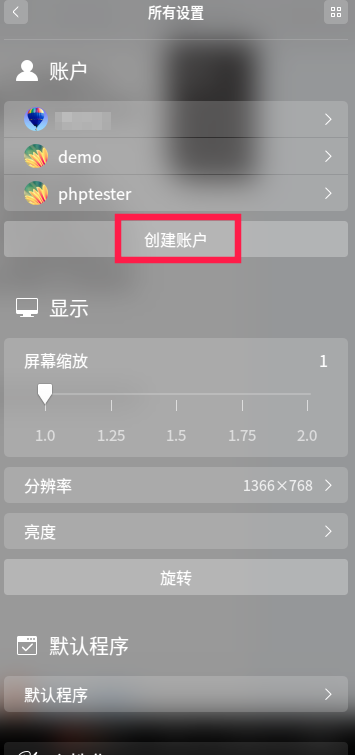
\includegraphics{images/manager-user-account-01.png}

\begin{figure}
\centering
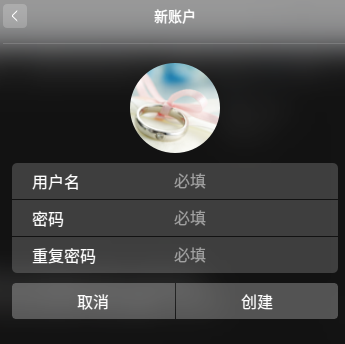
\includegraphics{images/manager-user-account-02.png}
\caption{图形方式创建账户}
\end{figure}

如果需要更改头像、设置全名、更改密码、设置是否自动登录免密码登录,可以选中需要修改的账户,点击进去就可以啦。

\begin{figure}
\centering
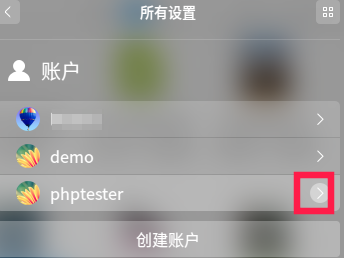
\includegraphics{images/manager-user-account-03.png}
\caption{图形方式配置账户}
\end{figure}

\begin{figure}
\centering
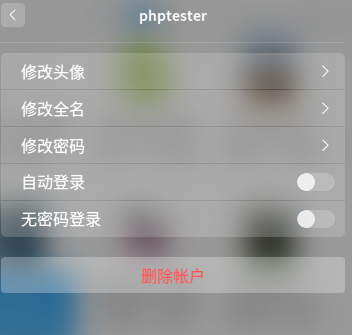
\includegraphics{images/manager-user-account-04.png}
\caption{图形方式配置账户}
\end{figure}

图形方式默认创建的账户是普通账户,比如是
\passthrough{\lstinline!phptester!} 账户,在
\emph{/etc/passwd},\emph{/etc/group} 会出现
\passthrough{\lstinline!phptester!}
相关的信息。有兴趣的读者,可以先去看看上述俩文件,后面还会对这俩文件作进一步的讲解。

\subsection{命令方式}

\partquote{运筹帷幄之中,决胜千里之外}{刘邦}
\partintro{
在服务器领域,Linux 无愧于操作系统中的王者,本部分介绍几个常见服务器软件的安装使用维护的方法。
}

\hypertarget{part:server-admin}{%
\part{服务器管理员}\label{part:server-admin}}

\hypertarget{chap:server-intro}{%
\chapter{\texorpdfstring{服务器\index{服务器}简介}{服务器简介}}\label{chap:server-intro}}

通过阅读本章,你将会了解到以下几项内容。

\begin{itemize}
\tightlist
\item
  管理 Linux 服务器
\item
  访问远程或局域网服务器
\item
  服务器的本地或远程日志记录
\item
  监控服务器
\item
  服务器的开启终止与状态查询
\end{itemize}

深度操作系统不仅仅是桌面办公的操作系统,还可以作为服务器使用。当然,也可根据自己的需要,用把深度桌面操作系统作为办公环境,另外安装个redhat/centos或者debian的服务器,以求更稳定的服务器。

\hypertarget{web-server-}{%
\chapter{Web Server 的搭建与运行}\label{web-server-}}

随着互联网技术的发展,网络开发越来越普及,越来越多的内容以网页的形式呈现。掌握一些网站服务器知识还是挺实用的。

\section{面向开发的一键安装类型}

前面我们提到了几个教学软件,

\section{关注效率稳定的搭建方法}

\hypertarget{-windows--samba-}{%
\chapter{\texorpdfstring{与 Windows\index{Windows} 共享文件打印机的
samba\index{samba}
服务}{与 Windows 共享文件打印机的 samba 服务}}\label{-windows--samba-}}

通过阅读本章,你将会了解到以下几项内容。

\begin{itemize}
\tightlist
\item
  深度系统如何跟Windows系统共享文件、打印机;
\item
  bash进行判断和简单数学计算
\item
  bash 的流程结构
\item
  实现把UC视频缓存变为普通视频文件的脚本
\end{itemize}

Windows
局域网中,为了方便互传文件或者打印,常常开启文件夹共享。在网上邻居里,能够看到其他人共享的文件夹,方便下载甚至上传。当前Windows局域网的通信工具也有一些,基本都支持文件互传,比如\href{http://www.feige360.com}{飞鸽传书}(跨平台支持苹果、Linux和安卓)、\href{www.imoffice.com}{imo内网通}、RTX腾讯通(貌似停更在\href{https://rtx.tencent.com/rtx/download/index.shtml}{2015版})、飞秋(貌似停更在\href{http://bbs.feiq18.com/config_nav.php?id=19}{2013版})、微软LYNC(貌似停更在\href{https://products.office.com/en-us/previous-versions/microsoft-lync-2013}{2013版})等。对于互联网,除了FTP、SCP和SSH外,QQ(深度系统自带),\href{http://akey.me/}{安司密信}、\href{https://www.dingtalk.com/}{钉钉}(暂时不支持Linux平台)等也是不错的选择。

但是,对于局域网的Deepin深度用户来讲,除了\href{https://github.com/iptux-src/iptux}{iptux信使}(只支持Linux、Mac,号称GNU/Linux版飞鸽传书)、\href{http://www.feige360.com/}{飞鸽传书}(最新版跨平台支持Linux)外,还可以安装samba
文件传输服务器。

\hypertarget{samba-}{%
\section{Samba 文件传输服务简介}\label{samba-}}

参考网页:

\begin{itemize}
\tightlist
\item
  \url{https://docs.microsoft.com/en-us/windows/desktop/FileIO/microsoft-smb-protocol-and-cifs-protocol-overview}
\item
  \url{https://www.cnblogs.com/LittleHann/p/6916326.html}
\end{itemize}

Samba 是一种网络文件共享的应用程序,基于微软制定的SMB(Server Message
Block)通信协议,被很多种操作系统,比如Windows、OS2、Linux等,作为CS(Client-Server客户端服务器端)的网络架构。通过基于SMB的samba,Linux系统就可以愉快的跟Windows系统共享文件和打印机。

在Samba的帮助下,Windows看Linux电脑的文件和打印机,仿佛就是自家的,反过来亦然。

\hypertarget{-samba-}{%
\section{深度自带 samba 的使用}\label{-samba-}}

参考网页:

\begin{itemize}
\tightlist
\item
  \url{https://wiki.deepin.org/wiki/\%E6\%B7\%B1\%E5\%BA\%A6\%E6\%96\%87\%E4\%BB\%B6\%E7\%AE\%A1\%E7\%90\%86\%E5\%99\%A8}
\end{itemize}

其实 samba
已经被\textbf{深度文件管理器}集成了。通过搜索深度文件管理的\href{https://github.com/linuxdeepin/dde-file-manager/search?q=samba\&unscoped_q=samba}{源码},会发现很多samba
相关的代码。也就是说,作为用户,我们不需要再单独安装samba服务了。

\subsection{共享本地文件}

\begin{enumerate}
\def\labelenumi{\arabic{enumi}.}
\tightlist
\item
  在文件管理器界面上,右键单击文件夹。
\item
  选择 共享文件夹。
\item
  勾选 共享此文件夹。
\item
  根据需要设置 共享名、权限 、匿名访问 后关闭标签。
\item
  在文件管理器界面上,点击 Icon\_menu 。
\item
  选择 设置共享密码。
\item
  输入共享密码。
\item
  点击 确定。
\end{enumerate}

\textbf{注意:}

\begin{enumerate}
\def\labelenumi{\arabic{enumi}.}
\tightlist
\item
  取消勾选 \textbf{共享此文件夹}
  可以取消文件共享,也可以右键单击文件,选择 \textbf{取消共享}。
\item
  有可能部分文件夹由于缺乏相应权限无法共享,请安装前面章节介绍更改权限的方法重新进行共享设置。
\end{enumerate}

\subsection{访问共享文件}

局域网中其他用户共享的文件一般都可以在网络邻居中找到,您也可以通过网络邻居访问共享文件。

\begin{enumerate}
\def\labelenumi{\arabic{enumi}.}
\tightlist
\item
  输入局域网用户的共享地址,按下键盘上的 Enter
  键。(如:\passthrough{\lstinline!smb://xxx.xxx.xxx.xxx/share!})
\item
  输入用户名密码或者匿名访问。

  \begin{enumerate}
  \def\labelenumii{\arabic{enumii})}
  \tightlist
  \item
    未加密的网络文件可以匿名访问,不需要输入用户名和密码。
  \item
    加密的网络文件会弹出登陆框,输入账号和密码之后才能访问。如果在用户名密码提示框中勾选
    \textbf{记住密码} ,再次访问不再需要密码。
  \end{enumerate}
\item
  点击 \textbf{连接}。
\end{enumerate}

\subsection{我的共享}

当您设置了共享文件时,我的共享图标将会出现在导航栏上,当所有共享文件都取消共享后,我的共享图标自动从侧边栏中移除。

\subsection{可能存在的小问题}

\setholdfigure

\BeginKnitrBlock{question}
共享失败,显示缺乏权限。
\EndKnitrBlock{question}
\BeginKnitrBlock{answer}
如果文件夹不是自己的,设置为共享会弹出如下的问题框,采用管理员权限打开文件夹,成功共享。当然也可以跟根据异常提示,修改或添加\emph{/etc/samba/smb.conf}的\passthrough{\lstinline!usershare owner only=false!}。

\begin{figure}
\centering
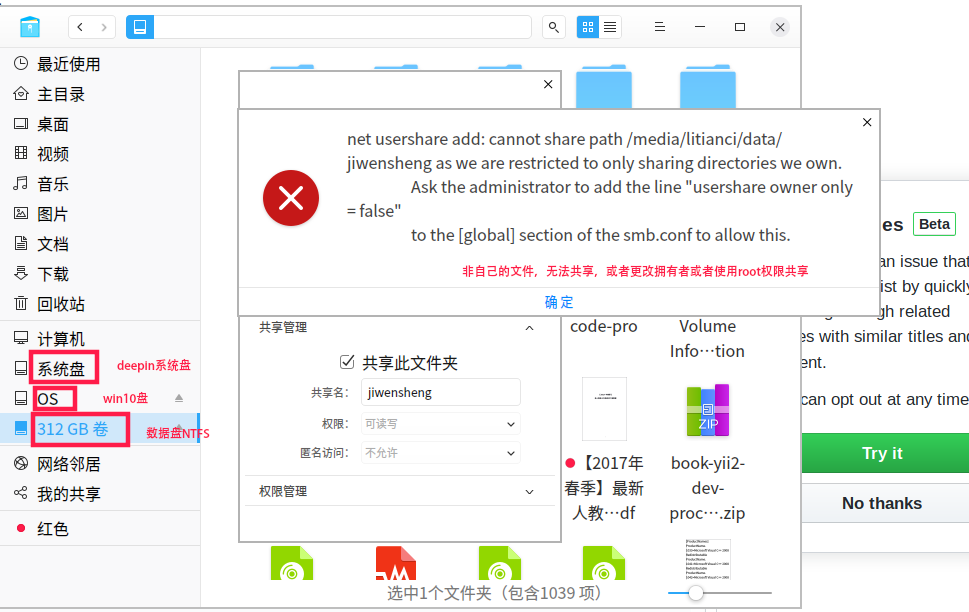
\includegraphics{images/samba-share.png}
\caption{共享文件夹出现的问题}
\end{figure}

由于权限的问题,取消共享也会出现类似问题,也请采用管理员权限或者修改配置文件的方法取消共享。

\begin{figure}
\centering
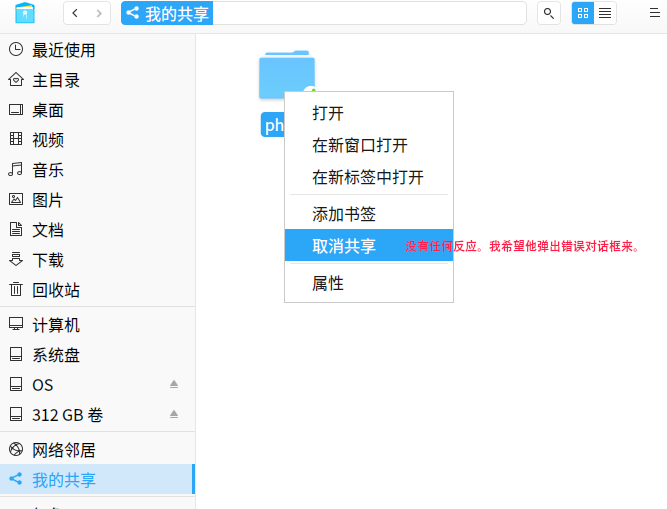
\includegraphics{images/samba-unshare.png}
\caption{取消共享出现的问题}
\end{figure}
\EndKnitrBlock{answer}
\setdefaultfigure

\hypertarget{-samba-}{%
\section{关于 samba 的配置}\label{-samba-}}

\subsection{手动安装}

如果你的操作系统不是 deepin,或者尚未自带 samba 服务,则需要先安装 samba
才可以使用其功能。安装方法很简单,

\begin{lstlisting}[language=bash]
# 如果您的操作系统是 centos 或者 Fedora,redhat 等。
$ sudo yum install samba -y
# 如果你的操作系统是 debian 系列,比如 ubuntu 等。
$ sudo apt-get install samba -y
# 其他版本的操作系统略。
\end{lstlisting}

\subsection{启动与停止}

因为深度采用的
\passthrough{\lstinline!systemctl!}控制服务,所以可以采用如下命令,

\begin{lstlisting}[language=bash]
$ sudo systemctl start smbd.service # 开启
$ sudo systemctl status smbd.service # 查看状态
$ systemctl status smbd # 查看状态不需要根权限
$ sudo systemctl stop smbd.service # 关闭
$ sudo systemctl restart smbd.service # 重启
\end{lstlisting}

其实\passthrough{\lstinline!smbd.service!}可以省略为\passthrough{\lstinline!smbd!}。当然,还可以用另外一种方式,直接调命令文件,启动这些命令。比如,

\begin{lstlisting}[language=bash]
$ sudo /etc/init.d/smbd start
\end{lstlisting}

这里是直接调用的\passthrough{\lstinline!smbd!}程序,最后的\passthrough{\lstinline!start!}可以换成\passthrough{\lstinline!stop!},\passthrough{\lstinline!status!}和\passthrough{\lstinline!restart!},效果跟上面\passthrough{\lstinline!systemctl!}的方式一致。对于\passthrough{\lstinline!status!}状态的查询,同样不需要root根权限。

对于\passthrough{\lstinline!redhat!}系列没有实测,查部分资料,把命令中\passthrough{\lstinline!smbd!}改为\passthrough{\lstinline!smb!}即可。

\subsection{配置文件}

Samba 的配置文件为\emph{/etc/samba/smb.conf}。

vim

\hypertarget{-u-file-}{%
\section{例:借助安卓软件 U-File 实现手机电脑互传}\label{-u-file-}}

本例是建立在局域网上的手机和电脑的互传,先介绍局域网的两种建立方法。如果您已经配置好了局域网,请跳过这一步。

\subsection{开启局域网}

可以使用手机开热点或者电脑开热点的方法。

由于本人所处工作环境电脑接触互联网不太方便,常用手机开热点的方法蹭网。手机开好热点后,电脑连接到相关无线网,在电脑命令行输入\passthrough{\lstinline!hostname -I!}会显示电脑的IP地址,本机为\passthrough{\lstinline!192.168.43.45!}。也可用通过手机端查看已经连接到热点设备的IP地址。

深度操作系统支持开启无线网热点。\textbf{控制中心}-\textgreater{}\textbf{网络}-\textgreater{}\textbf{热点}-\textgreater{}\textbf{热点设置},即可进入无线网设置页面,如图\ref{samba-hotwif}所示,

\begin{figure}
\centering
\includegraphics{images/samba-hotwifi.png}
\caption{开启无线网热点\label{samba-hotwif}}
\end{figure}

\partquote{三军之事,莫亲于间,赏莫厚于间,事莫密于间。非圣智不能用间,非仁义不能使间,非微妙不能得间之实。微哉!微哉!无所不用间也。}{孙武《孙子兵法 用间》}
\partintro{
古人云“千里之堤,溃于蚁穴”。害人之心不可有,防人之心不可无。作为系统使用者和管理者,必须牢牢绷紧安全这根弦。本部分简要的介绍一些安全常识,也只是避免一些小的安全隐患。更多知识,还需查阅更专业的安全书籍和资料。
}

\hypertarget{part:security}{%
\part{安全}\label{part:security}}

\hypertarget{chap:network-security}{%
\chapter{网络安全}\label{chap:network-security}}

本章您可以了解到,

\begin{itemize}
\tightlist
\item
  网络安全是啥
\end{itemize}

\partquote{这只是万里长征走完了第一步,以后的路程更长,工作更伟大,更艰苦。务必使同志们继续地保持谦虚、谨慎、不骄不躁的作风,务必使同志们继续地保持艰苦奋斗的作风。}{毛泽东}
\partintro{
\quad\quad 附录,首先引用了中国的一篇古文《愚公移山》,目的是告诉自己要坚持坚持再坚持;其次讲述了本书的制作步骤,方便后来人对模板进行改编和再创作;再次介绍了本书的大致框架设计,提醒需要注意的问题;再次列举了写作中常见的 \LaTeX 和 Bookdown 编写的示例;最后是常见问题解答以及本书的大事记。
}

\hypertarget{part:others}{%
\part{附录}\label{part:others}}

\hypertarget{chap:appendix}{%
\appendix}


\hypertarget{chap:yugong}{%
\chapter{\texorpdfstring{\index{愚公移山}愚公移山}{愚公移山}}\label{chap:yugong}}

\writeby{先秦 \quad 列御寇}

\begin{figure}
\centering
\includegraphics{images/yugongyishan.jpg}
\caption{徐悲鸿名画《愚公移山》}
\end{figure}

太行、 王屋二山, 方七百里, 高万仞, 本在冀州之南, 河阳之北。

北山愚公者, 年且九十, 面山而居。 惩山北之塞, 出入之迂也,
聚室而谋曰: \cqh 吾与汝毕力平险, 指通豫南, 达于汉阴,
可乎?\cqt  杂然相许。 其妻献疑曰: \cqh 以君之力, 曾不能损魁父之丘,
如太行、 王屋何? 且焉置土石?\cqt  杂曰: \cqh 投诸渤海之尾,
隐土之北。\cqt  遂率子孙荷担者三夫, 叩石垦壤, 箕畚运于渤海之尾。
邻人京城氏之孀妻有遗男, 始龀, 跳往助之。 寒暑易节, 始一返焉。

河曲智叟笑而止之曰: \cqh 甚矣, 汝之不惠! 以残年余力,
曾不能毁山之一毛, 其如土石何?\cqt  北山愚公长息曰: \cqh 汝心之固,
固不可彻, 曾不若孀妻弱子。 虽我之死, 有子存焉; 子又生孙, 孙又生子;
子又有子, 子又有孙; 子子孙孙无穷匮也, 而山不加增,
何苦而不平?\cqt  河曲智叟亡以应。

操蛇之神闻之, 惧其不已也, 告之于帝。 帝感其诚, 命夸娥氏二子负二山,
一厝朔东, 一厝雍南。 自此, 冀之南, 汉之阴, 无陇断焉。

\hypertarget{chap:makebook}{%
\chapter{如何制作本书}\label{chap:makebook}}

\section{准备工作}

本模板使用 bookdown 实现了由 R Markdown (Bookdown) -\textgreater{}
Markdown (Pandoc 标准) -\textgreater{} \LaTeX -\textgreater{} PDF
的一系列转换,其中用到的依赖有:

\begin{itemize}
\tightlist
\item
  R
\item
  pandoc
\item
  xetex
\end{itemize}

需要安装这些软件,才可以使用。

\hypertarget{linux-}{%
\subsection{Linux 下使用}\label{linux-}}

下面以深度操作系统15.5版本为例说明。安装过程中,请确保当前
\passthrough{\lstinline!rstudio!} 的版本高于 1.0.0,
\passthrough{\lstinline!texlive!} 为2015年后的版本,
\passthrough{\lstinline!pandoc!} 的版本高于 2.0.0。

\begin{lstlisting}[language=bash, numbers=none]
$ sudo apt-get install r-base r-base-dev \
rstudio texlive-full pandoc make
\end{lstlisting}

如果不能满足,请参考相关软件官网,下载最新版本。我的\href{https://my.oschina.net/bubifengyun/blog/1936119}{博客}记录了如何安装最新版
texlive,有需要的可以去看看。\href{https://github.com/jgm/pandoc/blob/master/INSTALL.md}{pandoc官网}有其安装教程。R
语言的安装方法\href{https://mirrors.tuna.tsinghua.edu.cn/CRAN/}{官网镜像}也可找到,这里就不赘述了,有问题可以邮件联系。

曾经在 Lubuntu 下试着安装过。一般先安装
\passthrough{\lstinline!make!},运行命令,仍旧出错,提示没有\passthrough{\lstinline!RScript!},接着安装\passthrough{\lstinline!r-base r-base-dev!}。再接着,\passthrough{\lstinline!sudo make!}还是出错。最后是\passthrough{\lstinline!pandoc!}版本问题了。由于
Lubuntu 版本太老,没能更新好。总结一下,

\begin{lstlisting}[language=bash, numbers=none]
$ sudo apt-get install make r-base r-base-dev -y
$ sudo make
\end{lstlisting}

第一次编译,可能需要安装很多软件,请静静等待。后面,直接运行下面这条语句,实现编译。

\begin{lstlisting}[language=bash, numbers=none]
$ make
\end{lstlisting}

\hypertarget{windows-}{%
\subsection{Windows 下使用}\label{windows-}}

略

\subsection{苹果操作系统下使用}

略

\section{编译模板}

\hypertarget{-}{%
\subsection{第一种编译方法 ------ 命令行编译}\label{-}}

模板默认使用GNUMake构建,后续如无特殊说明,默认执行命令的文件夹以及当前文件夹均为本模板的根目录。对于部分用户,第一次编译可能需要下载很多文件,最好联网编译,简言之\textbf{首次编译请联网}。如果第一次编译成功,后面再次编译则不需要联网。

\begin{lstlisting}[language=bash, numbers=none]
$ make
\end{lstlisting}

\hypertarget{-rstudio}{%
\subsection{第二种编译方法 ------ RStudio编译}\label{-rstudio}}

在已经安装 RStudio 的前提下,也可手动编译。打开 RStudio
软件,在弹出的界面,左上角点击 File-\textgreater{}Open Project,选中
\emph{./deepin-bible.Rproj} 文件打开,点击右上角靠下的一栏,有个
\passthrough{\lstinline!Build!} 格,会出现
\passthrough{\lstinline!Build Book!} 等按钮。 点击
\passthrough{\lstinline!Build Book!} 就会生成 PDF 书籍了,位于
\emph{./\_book/deepin-bible.pdf}
。本质上讲,第二种编译方法是调用的第一种编译方法,只不过方便懒得写命令行的用户。

\subsection{字数统计}

如果需要统计字数,先生成文件,然后执行如下命令,特别提醒\textbf{先编译书籍才可以统计字数}。

\begin{lstlisting}[language=bash, numbers=none]
$ make wordcount
\end{lstlisting}

\hypertarget{-r-}{%
\subsection{本书编译的 R 各包信息}\label{-r-}}

\begin{lstlisting}
## R version 3.4.4 (2018-03-15)
## Platform: x86_64-pc-linux-gnu (64-bit)
## Running under: Deepin 15
## 
## Matrix products: default
## BLAS: /usr/lib/x86_64-linux-gnu/blas/libblas.so.3.8.0
## LAPACK: /usr/lib/x86_64-linux-gnu/lapack/liblapack.so.3.8.0
## 
## locale:
##  [1] LC_CTYPE=zh_CN.UTF-8      
##  [2] LC_NUMERIC=C              
##  [3] LC_TIME=en_US.UTF-8       
##  [4] LC_COLLATE=zh_CN.UTF-8    
##  [5] LC_MONETARY=zh_CN.UTF-8   
##  [6] LC_MESSAGES=zh_CN.UTF-8   
##  [7] LC_PAPER=zh_CN.UTF-8      
##  [8] LC_NAME=C                 
##  [9] LC_ADDRESS=C              
## [10] LC_TELEPHONE=C            
## [11] LC_MEASUREMENT=zh_CN.UTF-8
## [12] LC_IDENTIFICATION=C       
## 
## attached base packages:
## [1] stats     graphics  grDevices utils     datasets 
## [6] base     
## 
## other attached packages:
## [1] knitr_1.20
## 
## loaded via a namespace (and not attached):
##  [1] compiler_3.4.4  backports_1.1.2 magrittr_1.5   
##  [4] bookdown_0.7.13 rprojroot_1.3-2 htmltools_0.3.6
##  [7] tools_3.4.4     rstudioapi_0.7  yaml_2.2.0     
## [10] Rcpp_0.12.18    stringi_1.2.4   rmarkdown_1.10 
## [13] methods_3.4.4   stringr_1.3.1   digest_0.6.17  
## [16] xfun_0.3        evaluate_0.11
\end{lstlisting}

\section{文件布局}

使用 \passthrough{\lstinline!tree!}
命令所得。为了篇幅,删除了部分文件名。

\begin{lstlisting}[caption=模板文件布局, label={intro:folder}, numbers=none]
.
├── bib
│   ├── book.bib
│   └── packages.bib
├── bin
│   ├── linux_x64
│   └── linux_x86
├── _bookdown.yml
├── css
│   └── style.css
├── deepin-bible.Rproj
├── images
│   ├── about-us_img-2.jpg
│   └── zhifubaozhifu.png
├── imakeidx.ist
├── index.Rmd
├── latex
│   ├── content.tex
│   └── template.tex
├── LICENSE
├── Makefile
├── _output.yml
├── README.md
├── _render.R
├── rmd
│   ├── 000-intro.Rmd
│   └── 899-appendix-history.Rmd
├── sjtuthesis.cfg
└── sjtuthesis.cls
\end{lstlisting}

\section{主要文件介绍}

\subsection{\texorpdfstring{\LaTeX 模板文件}{模板文件}}

格式控制文件控制着论文的表现形式,包括 \emph{./sjtuthesis.cfg} 和
\emph{./sjtuthesis.cls}。
其中,\cqh cls\cqt 控制论文主体格式,\cqh cfg\cqt 为配置文件。上述文件全部来自最新(2018-12-12)\href{https://github.com/sjtug/SJTUThesis}{上海交通大学学位论文
\LaTeX 模板}

\subsection{各章源文件}

主要位于 \emph{./rmd/} 文件夹。另外目录和模板的内容以 \LaTeX 形式存放在
\emph{./latex/} 文件夹下。各文件的详细说明见第\ref{chap:chapters}章。

\hypertarget{-1}{%
\subsection{配置文件}\label{-1}}

主要为 \emph{./index.Rmd}
文件,另外两个配置文件(\emph{./\_bookdown.yml}、\emph{./\_output.yml})没有特殊需求不需要更改。

对于 \emph{./index.Rmd}
文件,书名、作者等信息直接更改为自己的即可。由于本文采用的上海交大论文模板,一些配置不建议修改。如果想修改书籍字体,比如
\passthrough{\lstinline!classoption: [doctor, openright, twoside, fontset=adobe]!}
,就表示中文字体修改为 adobe
系列的字体。可供选择的中文字体:fandol(Fandol 开源字体)、windows(Windows
系统下的中文字体)、mac(macOS 系统下的华文字体)、ubuntu(Ubuntu
系统下的文泉驿和文鼎字体)、adobe(Adobe
公司的中文字体)、founder(方正公司的中文字体),默认根据操作系统自动配置。

如果打算使用本文的英文模板,可采用如下方式,在\passthrough{\lstinline!classoption: [doctor, openright, twoside, fontset=adobe]!}添加
``english'',比如\passthrough{\lstinline!classoption: [doctor, openright, twoside, fontset=adobe, english]!}。

\hypertarget{intro:fig}{%
\subsection{图片文件夹 images}\label{intro:fig}}

images
文件夹放置了需要插入文档中的图片文件(支持PNG/JPG/PDF/EPS格式的图片),可以在按照章节划分子目录。
模板文件中使用\passthrough{\lstinline!\\graphicspath!}命令定义了图片存储的顶层目录,在插入图片时,顶层目录名\cqh images\cqt 可省略。

\hypertarget{intro:bib}{%
\subsection{参考文献数据库bib}\label{intro:bib}}

目前参考文件数据库目录只存放一个参考文件数据库 \emph{./bib/book.bib},而
\emph{./bib/packages.bib} 是书籍编译参考的包信息。
关于参考文献引用,可参考附录\ref{chap:latex}中的例子。

\subsection{辅助文件}

\begin{itemize}
\tightlist
\item
  \emph{./deepin-bible.Rproj} 项目文件,方便使用 rstudio
  打开,如果仅使用 \passthrough{\lstinline!make!},可以不要。
\item
  \emph{./\_render.R}
  渲染文件,复制自\href{https://github.com/yihui/bookdown-chinese}{谢益辉Bookdown中文模板},致谢。
\item
  \emph{./Makefile} \passthrough{\lstinline!make!}
  的文件,综合\href{https://github.com/sjtug/SJTUThesis}{上海交通大学学位论文
  \LaTeX 模板}和\href{https://github.com/yihui/bookdown-chinese}{谢益辉Bookdown中文模板}。
\item
  \emph{./\_book/} 最终生成文件所在文件夹。
\item
  \emph{./\_bookdown\_files/} 过程中生成的文件所在文件夹。
\item
  \emph{./bin/},\emph{./imakeidx.ist} 是索引引擎及索引模板文件。
\item
  \emph{./css/} 用于生成非 PDF 书籍的模板,编译本书暂时用不到。
\end{itemize}

\hypertarget{chap:chapters}{%
\chapter{各章格式说明}\label{chap:chapters}}

Bookdown 编译各 \passthrough{\lstinline!Rmd!}
文件时,是按照文件名的字母排序拼接在一起的,故而我们不需要专门写一个文件来组织各章节,但是为了更好的利用这一排序规则,需要对文件名稍作调整。本模板的文件名采用如下命名方式,
\passthrough{\lstinline!xxx-name.Rmd!}。其中
\passthrough{\lstinline!xxx!} 表示从 \passthrough{\lstinline!000!} 到
\passthrough{\lstinline!999!},第一位表示第几部分,后两位如果为
\passthrough{\lstinline!00!}
表示该部分的简介,如果是其他数字则表示章节。\passthrough{\lstinline!name!}
是对应章节的名字。一章一个文件。

由于自身水平所限,部分格式实现起来费劲,就采用直接书写
\LaTeX 代码的形式实现了。

\section{章:前言}

前言作为一章,不属于书主体内容,位于本书开头,需要一些特殊设定。命名为\emph{./rmd/000-intro.Rmd}。
样式如下,

\begin{lstlisting}[caption=前言示例, label={chapters:intro}]
\frontmatter
\pagestyle{main}

# 前言

为什么要写这本书呢?起源于去武汉参观辛亥革命博物馆。

% 目录、插图目录、表格目录
\tableofcontents
\listoffigures
\addcontentsline{toc}{chapter}{\listfigurename}     % 将插图目录加入全文目录
\listoftables
\addcontentsline{toc}{chapter}{\listtablename}      % 将表格目录加入全文目录
\listofalgorithms
\addcontentsline{toc}{chapter}{\listalgorithmname}  % 将算法目录加入全文目录
\end{lstlisting}

\textbf{解释}

\begin{enumerate}
\def\labelenumi{\arabic{enumi}.}
\tightlist
\item
  第1、2行,表示下面属于前言部分,采用\textbf{罗马数字对前言编号},页面格式属于正文格式。
\item
  第4、6行,表示前言内容。
\item
  第8行,表示接下来为目录部分。
\item
  为了减少文件个数,把文件格式以及目录也放在该文件了,但也造成了文件不专用的问题。请根据爱好,自行斟酌。
\end{enumerate}

\section{前言后的部分章节}

前言后的部分章节,属于标准的 Markdown
文件,框架示例如代码\ref{chapters:frontword:nonhead}所示。

\begin{lstlisting}[caption=前言后文示例, label={chapters:frontword:nonhead}]
# 作者简介 {#author}

这将是是一群深度操作系统爱好者的杰作!!!
\end{lstlisting}

\textbf{解释}

\begin{enumerate}
\def\labelenumi{\arabic{enumi}.}
\tightlist
\item
  第1行,标准 Markdown 语句,表示这是一章。
\item
  第3行,该章的具体内容,可以使用 \LaTeX 或 Markdown 格式书写。
\end{enumerate}

\section{部分:第一部分简介}

\begin{lstlisting}[caption=第一部分简介示例, label={sec:mainpage:firstparthead}]
\mainmatter
\pagestyle{main}

\partquote{合抱之木,生于毫末;九层之台,起于垒土;千里之行,始于足下。}{老 \quad 子}

\partintro{
\quad\quad “话说天下大势,分久必合,合久必分”。
}

# (PART) Linux 及 Deepin 入门 {#part:intro -}
\end{lstlisting}

\textbf{解释}

\begin{enumerate}
\def\labelenumi{\arabic{enumi}.}
\tightlist
\item
  第1、2行,表示下面属于本文正文部分,采用\textbf{阿拉伯数字对正文编号},页面格式属于正文格式。
\item
  第4行,用于添加第一部分简介的名言警句。
\item
  第6-8行,表示第一部分简介的具体内容。
\item
  第10行,表示第一部分名称为\textbf{Linux 及 Deepin 入门},标签为
  \passthrough{\lstinline!part:intro!}。
\end{enumerate}

\section{各部分内部的章}

框架格式类似前言后的文件,如代码\ref{chapters:frontword:nonhead}所示,略。

\section{部分:附录及其他}

\begin{lstlisting}[caption=附录及其他部分框架示例, label={sec:appendix:head}]
\partquote{这只是万里长征走完了第一步,以后的路程更长,工作更伟大,更艰苦。务必使同志们继续地保持谦虚、谨慎、不骄不躁的作风,务必使同志们继续地保持艰苦奋斗的作风。}{毛泽东}
\partintro{
\quad\quad 附录及其他部分,首先引用了中国的一篇古文《愚公移山》,目的是告诉自己要坚持坚持再坚持;其次讲述了本书的制作步骤,方便后来人对模板进行改编和再创作;再次介绍了本书的大致框架设计,提醒需要注意的问题;再次列举了写作中常见的 \LaTeX 和 Bookdown 编写的示例;最后是常见问题解答以及本书的大事记。
}
# (PART) 附录及其他 {#part:others -}

# (APPENDIX) 附录 {#chap:appendix -} 
\end{lstlisting}

\textbf{解释}

\begin{enumerate}
\def\labelenumi{\arabic{enumi}.}
\tightlist
\item
  第1-5行,同框架示例\ref{sec:mainpage:firstparthead} 的介绍。
\item
  第7行,表示下面属于论文附录部分,采用\textbf{天干顺序对附录编号}。
\end{enumerate}

\section{附录内部各章}

框架格式类似前言后的文件,如代码\ref{chapters:frontword:nonhead}所示,略。

\section{后缀部分}

相关代码为 \LaTeX 形式,包括索引和参考文献等,由模板自动生成,不用关心。

\chapter{兼容 {\LaTeX} 排版}
\label{chap:latex}

\textbf{本章完全照抄交大论文模板的
\LaTeX 排版例子,除了动了标题和多了这行话,运行良好,但是部分地方会多出括号来,请对照原文删除。}

\section{列表环境}
\label{sec:list}

\subsection{无序列表}
\label{sec:unorderlist}

以下是一个无序列表的例子,列表的每个条目单独分段。

\begin{itemize}
  \item 这是一个无序列表。
  \item 这是一个无序列表。
  \item 这是一个无序列表。
\end{itemize}

使用\verb+itemize*+环境可以创建行内无序列表。

\begin{itemize*}
  \item 这是一个无序列表。
  \item 这是一个无序列表。
  \item 这是一个无序列表。
\end{itemize*}

行内无序列表条目不单独分段,所有内容直接插入在原文的段落中。

\subsection{有序列表}
\label{sec:orderlist}

使用环境\verb+enumerate+和\verb+enumerate*+创建有序列表,
使用方法无序列表类似。

\begin{enumerate}
  \item 这是一个有序列表。
  \item 这是一个有序列表。
  \item 这是一个有序列表。
\end{enumerate}

使用\verb+enumerate*+环境可以创建行内有序列表。

\begin{enumerate*}
  \item 这是一个默认有序列表。
  \item 这是一个默认有序列表。
  \item 这是一个默认有序列表。
\end{enumerate*}

行内有序列表条目不单独分段,所有内容直接插入在原文的段落中。

\subsection{描述型列表}

使用环境\verb+description+可创建带有主题词的列表,条目语法是\verb+\item[主题] 内容+。

\begin{description}
    \item[主题一] 详细内容
    \item[主题二] 详细内容
    \item[主题三] 详细内容 \ldots
\end{description}

\subsection{自定义列表样式}

可以使用\verb+label+参数控制列表的样式,
详细可以参考WikiBooks\footnote{\url{https://en.wikibooks.org/wiki/LaTeX/List_Structures\#Customizing_lists}}。
比如一个自定义样式的行内有序列表

\begin{enumerate*}[label=\itshape\alph*)\upshape]
  \item 这是一个自定义样式有序列表。
  \item 这是一个自定义样式有序列表。
  \item 这是一个自定义样式有序列表。
\end{enumerate*}

\section{数学排版}
\label{sec:matheq}

\subsection{公式排版}
\label{sec:eqformat}

这里有举一个长公式排版的例子,来自\href{http://www.tex.ac.uk/tex-archive/info/math/voss/mathmode/Mathmode.pdf}{《Math mode》}:

\begin {multline}
  \frac {1}{2}\Delta (f_{ij}f^{ij})=
  2\left (\sum _{i<j}\chi _{ij}(\sigma _{i}-
    \sigma _{j}) ^{2}+ f^{ij}\nabla _{j}\nabla _{i}(\Delta f)+\right .\\
  \left .+\nabla _{k}f_{ij}\nabla ^{k}f^{ij}+
    f^{ij}f^{k}\left [2\nabla _{i}R_{jk}-
      \nabla _{k}R_{ij}\right ]\vphantom {\sum _{i<j}}\right )
\end{multline}

\subsection{SI单位}

使用\verb+siunitx+宏包可以方便地输入SI单位制单位,例如\verb+\SI{5}{\um}+可以得到\SI{5}{\um}。

\subsubsection{一个四级标题}
\label{sec:depth4}

这是全文唯一的一个四级标题。在这部分中将演示了mathtools宏包中可伸长符号(箭头、等号的例子)的例子。

\begin{displaymath}
    A \xleftarrow[n=0]{} B \xrightarrow[LongLongLongLong]{n>0} C
\end{displaymath}

\begin{eqnarray}
  f(x) & \xleftrightarrow[]{A=B}  & B \\
  & \xleftharpoondown[below]{above} & B \nonumber \\
  & \xLeftrightarrow[below]{above} & B
\end{eqnarray}

又如:

\begin{align}
  \label{eq:none}
  & I(X_3;X_4)-I(X_3;X_4\mid{}X_1)-I(X_3;X_4\mid{}X_2) \nonumber \\
  = & [I(X_3;X_4)-I(X_3;X_4\mid{}X_1)]-I(X_3;X_4\mid{}\tilde{X}_2) \\
  = & I(X_1;X_3;X_4)-I(X_3;X_4\mid{}\tilde{X}_2)
\end{align}

\subsection{定理环境}

模板中定义了丰富的定理环境
algo(算法),thm(定理),lem(引理),prop(命题),cor(推论),defn(定义),conj(猜想),exmp(例),rem(注),case(情形),
bthm(断言定理),blem(断言引理),bprop(断言命题),bcor(断言推论)。
amsmath还提供了一个proof(证明)的环境。
这里举一个\cqh 定理\cqt 和\cqh 证明\cqt 的例子。

\begin{thm}[留数定理]
\label{thm:res}
  假设$U$是复平面上的一个单连通开子集,$a_1,\ldots,a_n$是复平面上有限个点,$f$是定义在$U\backslash \{a_1,\ldots,a_n\}$上的全纯函数,
  如果$\gamma$是一条把$a_1,\ldots,a_n$包围起来的可求长曲线,但不经过任何一个$a_k$,并且其起点与终点重合,那么:

  \begin{equation}
    \label{eq:res}
    \ointop_{\gamma}f(z)\,\mathrm{d}z = 2\uppi\mathbf{i}\sum^n_{k=1}\mathrm{I}(\gamma,a_k)\mathrm{Res}(f,a_k)
  \end{equation}

  如果$\gamma$是若尔当曲线,那么$\mathrm{I}(\gamma, a_k)=1$,因此:

  \begin{equation}
    \label{eq:resthm}
    \ointop_{\gamma}f(z)\,\mathrm{d}z = 2\uppi\mathbf{i}\sum^n_{k=1}\mathrm{Res}(f,a_k)
  \end{equation}

      % \oint_\gamma f(z)\, dz = 2\pi i \sum_{k=1}^n \mathrm{Res}(f, a_k ).

  在这里,$\mathrm{Res}(f, a_k)$表示$f$在点$a_k$的留数,$\mathrm{I}(\gamma,a_k)$表示$\gamma$关于点$a_k$的卷绕数。
  卷绕数是一个整数,它描述了曲线$\gamma$绕过点$a_k$的次数。如果$\gamma$依逆时针方向绕着$a_k$移动,卷绕数就是一个正数,
  如果$\gamma$根本不绕过$a_k$,卷绕数就是零。

  定理\ref{thm:res}的证明。

  \begin{proof}
    首先,由……

    其次,……

    所以……
  \end{proof}
\end{thm}

上面的公式例子中,有一些细节希望大家注意。微分号d应该使用\cqh 直立体\cqt 也就是用mathrm包围起来。
并且,微分号和被积函数之间应该有一段小间隔,可以插入\verb+\,+得到。
斜体的\(d\)通常只作为一般变量。
i,j作为虚数单位时,也应该使用\cqh 直立体\cqt 为了明显,还加上了粗体,例如\verb+\mathbf{i}+。斜体\(i,j\)通常用作表示\cqh 序号\cqt 。
其他字母在表示常量时,也推荐使用\cqh 直立体\cqt 譬如,圆周率\(\uppi\)(需要upgreek宏包),自然对数的底\(\mathrm{e}\)。
不过,我个人觉得斜体的\(e\)和\(\pi\)很潇洒,在不至于引起混淆的情况下,我也用这两个字母的斜体表示对应的常量。

\section{向文档中插入图像}
\label{sec:insertimage}

\subsection{支持的图片格式}
\label{sec:imageformat}

\XeTeX 可以很方便地插入PDF、PNG、JPG格式的图片。

插入PNG/JPG的例子如\ref{fig:SRR}所示。
这两个水平并列放置的图共享一个\cqh 图标题\cqt (table
caption),没有各自的小标题。

\begin{figure}[!htp]
  \centering
  \includegraphics[width=4cm]{example/sjtulogo.png}
  \hspace{1cm}
  \includegraphics[width=4cm]{example/sjtulogo.jpg}
  \bicaption[这里将出现在插图索引中]
    {中文题图}
    {English caption}
  \label{fig:SRR}
\end{figure}

这里还有插入EPS图像和PDF图像的例子,如图\ref{fig:epspdf:a}和图\ref{fig:epspdf:b}。这里将EPS和PDF图片作为子图插入,每个子图有自己的小标题。子图标题使用subcaption宏包添加。

\begin{figure}[!htp]
  \centering
  \subcaptionbox{EPS 图像\label{fig:epspdf:a}}[3cm] %标题的长度,超过则会换行,如下一个小图。
    {\includegraphics[height=2.5cm]{example/sjtulogo.eps}}
  \hspace{4em}
  \subcaptionbox{PDF 图像,注意这个图略矮些。如果标题很长的话,它会自动换行\label{fig:epspdf:b}}
    {\includegraphics[height=2cm]{sjtulogo.pdf}}
  \bicaption{插入eps和pdf的例子(使用 subcaptionbox 方式)}{An EPS and PDF demo with subcaptionbox}
  \label{fig:pdfeps-subcaptionbox}
\end{figure}

\begin{figure}[!htp]
  \centering
  \begin{subfigure}{2.5cm}
    \centering
    \includegraphics[height=2.5cm]{example/sjtulogo.eps}
    \caption{EPS 图像}
  \end{subfigure}
  \hspace{4em}
  \begin{subfigure}{0.4\textwidth}
    \centering
    \includegraphics[height=2cm]{sjtulogo.pdf}
    \caption{PDF 图像,注意这个图略矮些。subfigure中同一行的子图在顶端对齐。}
  \end{subfigure}
  \bicaption{插入eps和pdf的例子(使用 subfigure 方式)}{An EPS and PDF demo with subfigure}
  \label{fig:pdfeps-subfigure}
\end{figure}

更多关于
\LaTeX 插图的例子可以参考\href{http://www.cs.duke.edu/junhu/Graphics3.pdf}{《\LaTeX 插图指南》}。

\subsection{长标题的换行}
\label{sec:longcaption}

图\ref{fig:longcaptionbad}和图\ref{fig:longcaptiongood}都有比较长图标题,通过对比发现,图\ref{fig:longcaptiongood}的换行效果更好一些。
其中使用了minipage环境来限制整个浮动体的宽度。

\begin{figure}[!htp]
  \centering
  \includegraphics[width=4cm]{sjtubadge.pdf}
  \bicaption[这里将出现在插图索引]
    {上海交通大学是我国历史最悠久的高等学府之一,是教育部直属、教育部与上海市共建的全国重点大学.}
    {Where there is a will, there is a way.}
 \label{fig:longcaptionbad}
\end{figure}

\begin{figure}[!htbp]
  \centering
  \begin{minipage}[b]{0.6\textwidth}
    \centering
    \includegraphics[width=4cm]{sjtubadge.pdf}
    \bicaption[出现在插图索引中]
      {上海交通大学是我国历史最悠久的高等学府之一,是教育部直属、教育部与上海市共建的全国重点大学.}
      {Where there is a will, there is a way.}
    \label{fig:longcaptiongood}
  \end{minipage}
\end{figure}

\subsection{添加图注}

当插图中组成部件由数字或字母等编号表示时,可在插图下方添加图注进行说明,如图\ref{fig:cn_100t}所示。

\begin{figure}[!htp]
  \centering
  \includegraphics[width=0.3\textwidth]{example/cn_100t.png}\
  \begin{center}
    \small\kaishu 1.立柱 2.提升释放机构 3.标准冲击加速度计 \\ 4.导轨 5.重锤 6.被校力传感器 7.底座
  \end{center}
  \vspace{-1em}
  \bicaption[出现在插图索引中]
    {示例图片来源于\parencite{he1999}}
    {Stay hungry, stay foolish.}
 \label{fig:cn_100t}
\end{figure}

\subsection{绘制流程图}

图\ref{fig:flow_chart}是一张流程图示意。使用tikz环境,搭配四种预定义节点(\verb+startstop+、\verb+process+、\verb+decision+和\verb+io+),可以容易地绘制出流程图。

\begin{figure}[!htp]
    \centering
    \resizebox{6cm}{!}{\begin{tikzpicture}[node distance=2cm]
    \node (pic) [startstop] {待测图片};
    \node (bg) [io, below of=pic] {读取背景};
    \node (pair) [process, below of=bg] {匹配特征点对};
    \node (threshold) [decision, below of=pair, yshift=-0.5cm] {多于阈值};
    \node (clear) [decision, right of=threshold, xshift=3cm] {清晰?};
    \node (capture) [process, right of=pair, xshift=3cm, yshift=0.5cm] {重采};
    \node (matrix_p) [process, below of=threshold, yshift=-0.8cm] {透视变换矩阵};
    \node (matrix_a) [process, right of=matrix_p, xshift=3cm] {仿射变换矩阵};
    \node (reg) [process, below of=matrix_p] {图像修正};
    \node (return) [startstop, below of=reg] {配准结果};
     
    %连接具体形状
    \draw [arrow](pic) -- (bg);
    \draw [arrow](bg) -- (pair);
    \draw [arrow](pair) -- (threshold);

    \draw [arrow](threshold) -- node[anchor=south] {否} (clear);

    \draw [arrow](clear) -- node[anchor=west] {否} (capture);
    \draw [arrow](capture) |- (pic);
    \draw [arrow](clear) -- node[anchor=west] {是} (matrix_a);
    \draw [arrow](matrix_a) |- (reg);

    \draw [arrow](threshold) -- node[anchor=east] {是} (matrix_p);
    \draw [arrow](matrix_p) -- (reg);
    \draw [arrow](reg) -- (return);
\end{tikzpicture}
}
    \bicaption{绘制流程图效果}{Flow chart}
    \label{fig:flow_chart}
\end{figure}

\clearpage

\section{表格}
\label{sec:tab}

这一节给出的是一些表格的例子,如表\ref{tab:firstone}所示。

\begin{table}[!hpb]
  \centering
  \bicaption[指向一个表格的表目录索引]
    {一个颇为标准的三线表格\footnotemark[1]}
    {A Table}
  \label{tab:firstone}
  \begin{tabular}{@{}llr@{}} \toprule
    \multicolumn{2}{c}{Item} \\ \cmidrule(r){1-2}
    Animal & Description & Price (\$)\\ \midrule
    Gnat & per gram & 13.65 \\
    & each & 0.01 \\
    Gnu & stuffed & 92.50 \\
    Emu & stuffed & 33.33 \\
    Armadillo & frozen & 8.99 \\ \bottomrule
  \end{tabular}
\end{table}
\footnotetext[1]{这个例子来自\href{http://www.ctan.org/tex-archive/macros/latex/contrib/booktabs/booktabs.pdf}{《Publication quality tables in LATEX》}(booktabs宏包的文档)。这也是一个在表格中使用脚注的例子,请留意与threeparttable实现的效果有何不同。}

下面一个是一个更复杂的表格,用threeparttable实现带有脚注的表格,如表\ref{tab:footnote}。

\begin{table}[!htpb]
  \bicaption[出现在表目录的标题]
    {一个带有脚注的表格的例子}
    {A Table with footnotes}
  \label{tab:footnote}
  \centering
  \begin{threeparttable}[b]
     \begin{tabular}{ccd{4}cccc}
      \toprule
      \multirow{2}{6mm}{total}&\multicolumn{2}{c}{20\tnote{1}} & \multicolumn{2}{c}{40} &  \multicolumn{2}{c}{60}\\
      \cmidrule(lr){2-3}\cmidrule(lr){4-5}\cmidrule(lr){6-7}
      &www & \multicolumn{1}{c}{k} & www & k & www & k \\ % 使用说明符 d 的列会自动进入数学模式,使用 \multicolumn 对文字表头做特殊处理
      \midrule
      &$\underset{(2.12)}{4.22}$ & 120.0140\tnote{2} & 333.15 & 0.0411 & 444.99 & 0.1387 \\
      &168.6123 & 10.86 & 255.37 & 0.0353 & 376.14 & 0.1058 \\
      &6.761    & 0.007 & 235.37 & 0.0267 & 348.66 & 0.1010 \\
      \bottomrule
    \end{tabular}
    \begin{tablenotes}
    \item [1] the first note.% or \item [a]
    \item [2] the second note.% or \item [b]
    \end{tablenotes}
  \end{threeparttable}
\end{table}

\section{参考文献管理}

\LaTeX 具有将参考文献内容和表现形式分开管理的能力,涉及三个要素:参考文献数据库、参考文献引用格式、在正文中引用参考文献。
这样的流程需要多次编译:

\begin{enumerate}[noitemsep,topsep=0pt,parsep=0pt,partopsep=0pt]
    \item 用户将论文中需要引用的参考文献条目,录入纯文本数据库文件(bib文件)。
    \item 调用xelatex对论文模板做第一次编译,扫描文中引用的参考文献,生成参考文献入口文件(aux)文件。
    \item 调用bibtex,以参考文献格式和入口文件为输入,生成格式化以后的参考文献条目文件(bib)。
    \item 再次调用xelatex编译模板,将格式化以后的参考文献条目插入正文。
\end{enumerate}

参考文献数据库(thesis.bib)的条目,可以从Google
Scholar搜索引擎\footnote{\url{https://scholar.google.com}}、CiteSeerX搜索引擎\footnote{\url{http://citeseerx.ist.psu.edu}}中查找,文献管理软件Papers\footnote{\url{http://papersapp.com}}、Mendeley\footnote{\url{http://www.mendeley.com}}、JabRef\footnote{\url{http://jabref.sourceforge.net}}也能够输出条目信息。

下面是在Google Scholar上搜索到的一条文献信息,格式是纯文本:

\begin{lstlisting}[caption={从Google Scholar找到的参考文献条目}, label=googlescholar, escapeinside="", numbers=none]
    @phdthesis{"白2008信用风险传染模型和信用衍生品的定价",
      title={"信用风险传染模型和信用衍生品的定价"},
      author={"白云芬"},
      year={2008},
      school={"上海交通大学"}
    }
\end{lstlisting}

推荐修改后在bib文件中的内容为:

\begin{lstlisting}[caption={修改后的参考文献条目}, label=itemok, escapeinside="", numbers=none]
  @phdthesis{bai2008,
    title={"信用风险传染模型和信用衍生品的定价"},
    author={"白云芬"},
    date={2008},
    address={"上海"},
    school={"上海交通大学"}
  }
\end{lstlisting}

按照教务处的要求,参考文献外观应符合国标GBT7714的要求\footnote{\url{http://www.cces.net.cn/guild/sites/tmxb/Files/19798_2.pdf}}。
在模板中,表现形式的控制逻辑通过biblatex-gb7714-2015包实现\footnote{\url{https://www.ctan.org/pkg/biblatex-gb7714-2015}},基于\{Bib\LaTeX\}管理文献。在目前的多数TeX发行版中,可能都没有默认包含biblatex-gb7714-2015,需要手动安装。

正文中引用参考文献时,用\verb+\cite{key1,key2,key3...}+可以产生\cqh 上标引用的参考文献\cqt ,
如\cite{Meta_CN,chen2007act,DPMG}。
使用\verb+\parencite{key1,key2,key3...}+则可以产生水平引用的参考文献,例如\parencite{JohnD,zhubajie,IEEE-1363}。
请看下面的例子,将会穿插使用水平的和上标的参考文献:关于书的\parencite{Meta_CN,JohnD,IEEE-1363},关于期刊的\cite{chen2007act,chen2007ewi},
会议论文\parencite{DPMG,kocher99,cnproceed},
硕士学位论文\parencite{zhubajie,metamori2004},博士学位论文\cite{shaheshang,FistSystem01,bai2008},标准文件\parencite{IEEE-1363},技术报告\cite{NPB2},电子文献\parencite{xiaoyu2001, CHRISTINE1998},用户手册\parencite{RManual}。

总结一些注意事项:

\begin{itemize}
\item 参考文献只有在正文中被引用了,才会在最后的参考文献列表中出现;
\item 参考文献\cqh 数据库文件\cqt bib是纯文本文件,请使用UTF-8编码,不要使用GBK编码;
\item 参考文献条目中默认通过date域输入时间。兼容使用year域时会产生编译warning,可忽略。
\end{itemize}

\section{用listings插入源代码}

原先ctexbook文档类和listings宏包配合使用时,代码在换页时会出现莫名其妙的错误,后来经高人指点,顺利解决了。
感兴趣的话,可以看看\href{http://bbs.ctex.org/viewthread.php?tid=53451}{这里}。
这里给使用listings宏包插入源代码的例子,这里是一段C代码。
另外,listings宏包真可谓博大精深,可以实现各种复杂、漂亮的效果,想要进一步学习的同学,可以参考
\href{http://mirror.ctan.org/macros/latex/contrib/listings/listings.pdf}{listings宏包手册}。

\begin{lstlisting}[language={C}, caption={一段C源代码}]
#include <stdio.h>
#include <unistd.h>
#include <sys/types.h>
#include <sys/wait.h>

int main() {
  pid_t pid;

  switch ((pid = fork())) {
  case -1:
    printf("fork failed\n");
    break;
  case 0:
    /* child calls exec */
    execl("/bin/ls", "ls", "-l", (char*)0);
    printf("execl failed\n");
    break;
  default:
    /* parent uses wait to suspend execution until child finishes */
    wait((int*)0);
    printf("is completed\n");
    break;
  }

  return 0;
}
\end{lstlisting}

\section{用algorithm和algorithmicx宏包插入算法描述}

algorithmicx 比 algorithmic 增加了一些命令。
示例如算法\ref{algo:sum_100}和算法\ref{algo:merge_sort},
后者的代码来自\href{http://hustsxh.is-programmer.com/posts/38801.html}{xhSong的博客}。
algorithmicx的详细使用方法见\href{http://mirror.hust.edu.cn/CTAN/macros/latex/contrib/algorithmicx/algorithmicx.pdf}{官方README}。
使用算法宏包时,算法出现的位置很多时候不按照tex文件里的书写顺序,
需要强制定位时可以使用\verb+\begin{algorithm}[H]+
\footnote{http://tex.stackexchange.com/questions/165021/fixing-the-location-of-the-appearance-in-algorithmicx-environment}

这是写在算法\ref{algo:sum_100}前面的一段话,在生成的文件里它会出现在算法\ref{algo:sum_100}前面。

\begin{algorithm}
% \begin{algorithm}[H] % 强制定位
\caption{求100以内的整数和}
\label{algo:sum_100}
\begin{algorithmic}[1] %每行显示行号
\Ensure 100以内的整数和 % 输出
\State $sum \gets 0$
\For{$i = 0 \to 100$}
    \State $sum \gets sum + i$
  \EndFor
\end{algorithmic}
\end{algorithm}

这是写在两个算法中间的一段话,当算法\ref{algo:sum_100}不使用\verb+\begin{algorithm}[H]+时它也会出现在算法\ref{algo:sum_100}前面。

对于很长的算法,单一的算法块\verb+\begin{algorithm}...\end{algorithm}+是不能自动跨页的
\footnote{http://tex.stackexchange.com/questions/70733/latex-algorithm-not-display-under-correct-section},
会出现的情况有:

\begin{itemize}
  \item 该页放不下当前的算法,留下大片空白,算法在下一页显示
  \item 单一页面放不下当前的算法,显示时超过页码的位置直到超出整个页面范围
\end{itemize}

解决方法有:

\begin{itemize}
  \item (推荐)使用\verb+algstore{algname}+和\verb+algrestore{algname}+来讲算法分为两个部分\footnote{http://tex.stackexchange.com/questions/29816/algorithm-over-2-pages},如算法\ref{algo:merge_sort}。
  \item 人工拆分算法为多个小的部分。
\end{itemize}

\begin{algorithm}
% \begin{algorithm}[H] % 强制定位
\caption{用归并排序求逆序数}
\label{algo:merge_sort}
\begin{algorithmic}[1] %每行显示行号
\Require $Array$数组,$n$数组大小 % 输入
\Ensure 逆序数 % 输出
\Function {MergerSort}{$Array, left, right$}
  \State $result \gets 0$
  \If {$left < right$}
    \State $middle \gets (left + right) / 2$
    \State $result \gets result +$ \Call{MergerSort}{$Array, left, middle$}
    \State $result \gets result +$ \Call{MergerSort}{$Array, middle, right$}
    \State $result \gets result +$ \Call{Merger}{$Array,left,middle,right$}
  \EndIf
  \State \Return{$result$}
\EndFunction
\State %空一行
\Function{Merger}{$Array, left, middle, right$}
  \State $i\gets left$
  \State $j\gets middle$
  \State $k\gets 0$
  \State $result \gets 0$
  \While{$i<middle$ \textbf{and} $j<right$}
    \If{$Array[i]<Array[j]$}
      \State $B[k++]\gets Array[i++]$
    \Else
      \State $B[k++] \gets Array[j++]$
      \State $result \gets result + (middle - i)$
    \EndIf
  \EndWhile
  \algstore{MergeSort}
\end{algorithmic}
\end{algorithm}

\begin{algorithm}
\begin{algorithmic}[1]
  \algrestore{MergeSort}
  \While{$i<middle$}
    \State $B[k++] \gets Array[i++]$
  \EndWhile
  \While{$j<right$}
    \State $B[k++] \gets Array[j++]$
  \EndWhile
  \For{$i = 0 \to k-1$}
    \State $Array[left + i] \gets B[i]$
  \EndFor
  \State \Return{$result$}
\EndFunction
\end{algorithmic}
\end{algorithm}

这是写在算法\ref{algo:merge_sort}后面的一段话,
但是当算法\ref{algo:merge_sort}不使用\verb+\begin{algorithm}[H]+时它会出现在算法\ref{algo:merge_sort}
甚至算法\ref{algo:sum_100}前面。

对于算法的索引要注意\verb+\caption+和\verb+\label+的位置,
必须是先\verb+\caption+再\verb+\label+\footnote{http://tex.stackexchange.com/questions/65993/algorithm-numbering},
否则会出现\verb+\ref{algo:sum_100}+生成的编号跟对应算法上显示不一致的问题。

根据Werner的回答\footnote{http://tex.stackexchange.com/questions/53357/switch-cases-in-algorithmic}
增加了\verb+Switch+和\verb+Case+的支持,见算法\ref{algo:switch_example}。

\begin{algorithm}
\caption{Switch示例}
\label{algo:switch_example}
\begin{algorithmic}[1]
  \Switch{$s$}
    \Case{$a$}
      \Assert{0}
    \EndCase
    \Case{$b$}
      \Assert{1}
    \EndCase
    \Default
      \Assert{2}
    \EndDefault
  \EndSwitch
\end{algorithmic}
\end{algorithm}

\hypertarget{chap:rmarkdown}{%
\chapter{RMarkdown/Bookdown 排版示例}\label{chap:rmarkdown}}

本文无意全文翻译 RMarkdown/Bookdown
的使用方法,只是简单的复制,详细内容请参考页面:

\begin{itemize}
\tightlist
\item
  \url{https://rmarkdown.rstudio.com/lesson-1.html}
\item
  \url{https://bookdown.org/yihui/bookdown/}
\item
  \url{https://bookdown.org/yihui/bookdown/components.html}
\item
  \url{http://pandoc.org/}
\end{itemize}

以下为全文复制 \url{https://bookdown.org/yihui/bookdown/components.html}
,有改动。

This chapter demonstrates the syntax of common components of a book
written in \textbf{bookdown}, including code chunks, figures, tables,
citations, math theorems, and equations. The approach is based on
Pandoc, so we start with the syntax of Pandoc's\index{Pandoc} flavor of
Markdown.

\hypertarget{markdown-syntax}{%
\section{Markdown syntax}\label{markdown-syntax}}

In this section, we give a very brief introduction to Pandoc's
Markdown\index{Markdown}. Readers who are familiar with Markdown can
skip this section. The comprehensive syntax of Pandoc's Markdown can be
found on the Pandoc website \url{http://pandoc.org}.

\hypertarget{inline-formatting}{%
\subsection{Inline formatting}\label{inline-formatting}}

You can make text \emph{italic} by surrounding it with underscores or
asterisks, e.g., \passthrough{\lstinline!\_text\_!} or
\passthrough{\lstinline!*text*!}. For \textbf{bold} text, use two
underscores (\passthrough{\lstinline!\_\_text\_\_!}) or asterisks
(\passthrough{\lstinline!**text**!}). Text surrounded by
\passthrough{\lstinline!\~!} will be converted to a subscript (e.g.,
\passthrough{\lstinline!H\~2\~SO\~4\~!} renders
H\textsubscript{2}SO\textsubscript{4}), and similarly, two carets
(\passthrough{\lstinline!^!}) produce a superscript (e.g.,
\passthrough{\lstinline!Fe^2+^!} renders Fe\textsuperscript{2+}). To
mark text as \passthrough{\lstinline!inline code!}, use a pair of
backticks, e.g., \passthrough{\lstinline!`code`!}.\footnote{To include
  literal backticks, use more backticks outside, e.g., you can use two
  backticks to preserve one backtick inside:
  \passthrough{\lstinline!`` `code` ``!}.} Small caps can be produced by
the HTML tag \passthrough{\lstinline!span!}, e.g.,
\passthrough{\lstinline!<span style="font-variant:small-caps;">Small Caps</span>!}
renders \textsc{Small Caps}. Links are created using
\passthrough{\lstinline![text](link)!}, e.g.,
\passthrough{\lstinline![RStudio](https://www.rstudio.com)!}, and the
syntax for images is similar: just add an exclamation mark, e.g.,
\passthrough{\lstinline"![alt text or image title](path/to/image)"}.
Footnotes are put inside the square brackets after a caret
\passthrough{\lstinline!^[]!}, e.g.,
\passthrough{\lstinline!^[This is a footnote.]!}. We will talk about
citations in Section \ref{citations}.

\hypertarget{block-level-elements}{%
\subsection{Block-level elements}\label{block-level-elements}}

Section headers can be written after a number of pound signs, e.g.,

\begin{lstlisting}
# First-level header

## Second-level header

### Third-level header
\end{lstlisting}

If you do not want a certain heading to be numbered, you can add
\passthrough{\lstinline!\{-\}!} after the heading, e.g.,

\begin{lstlisting}
# Preface {-}
\end{lstlisting}

Unordered list items start with \passthrough{\lstinline!*!},
\passthrough{\lstinline!-!}, or \passthrough{\lstinline!+!}, and you can
nest one list within another list by indenting the sub-list by four
spaces, e.g.,

\begin{lstlisting}
- one item
- one item
- one item
    - one item
    - one item
\end{lstlisting}

The output is:

\begin{itemize}
\tightlist
\item
  one item
\item
  one item
\item
  one item

  \begin{itemize}
  \tightlist
  \item
    one item
  \item
    one item
  \end{itemize}
\end{itemize}

Ordered list items start with numbers (the rule for nested lists is the
same as above), e.g.,

\begin{lstlisting}
1. the first item
2. the second item
3. the third item
\end{lstlisting}

The output does not look too much different with the Markdown source:

\begin{enumerate}
\def\labelenumi{\arabic{enumi}.}
\tightlist
\item
  the first item
\item
  the second item
\item
  the third item
\end{enumerate}

Blockquotes are written after \passthrough{\lstinline!>!}, e.g.,

\begin{lstlisting}
> "I thoroughly disapprove of duels. If a man should challenge me,
  I would take him kindly and forgivingly by the hand and lead him
  to a quiet place and kill him."
>
> --- Mark Twain
\end{lstlisting}

The actual output (we customized the style for blockquotes in this
book):

\begin{quote}
``I thoroughly disapprove of duels. If a man should challenge me, I
would take him kindly and forgivingly by the hand and lead him to a
quiet place and kill him.''

\VA{--- Mark Twain}{}
\end{quote}

Plain code blocks can be written after three or more backticks, and you
can also indent the blocks by four spaces, e.g.,

\begin{lstlisting}
```
This text is displayed verbatim / preformatted
```

Or indent by four spaces:

    This text is displayed verbatim / preformatted
\end{lstlisting}

\hypertarget{math-expressions}{%
\subsection{Math expressions}\label{math-expressions}}

Inline LaTeX equations\index{LaTeX math expression} can be written in a
pair of dollar signs using the LaTeX syntax, e.g.,
\passthrough{\lstinline!$f(k) = \{n \\choose k\} p^\{k\} (1-p)^\{n-k\}$!}
(actual output: \(f(k)={n \choose k}p^{k}(1-p)^{n-k}\)); math
expressions of the display style can be written in a pair of double
dollar signs, e.g.,
\passthrough{\lstinline!$$f(k) = \{n \\choose k\} p^\{k\} (1-p)^\{n-k\}$$!},
and the output looks like this:

\[f\left(k\right)=\binom{n}{k}p^k\left(1-p\right)^{n-k}\]

You can also use math environments inside \passthrough{\lstinline!$ $!}
or \passthrough{\lstinline!$$ $$!}, e.g.,

\begin{lstlisting}[language=TeX]
$$\begin{array}{ccc}
x_{11} & x_{12} & x_{13}\\
x_{21} & x_{22} & x_{23}
\end{array}$$
\end{lstlisting}

\[\begin{array}{ccc}
x_{11} & x_{12} & x_{13}\\
x_{21} & x_{22} & x_{23}
\end{array}\]

\begin{lstlisting}[language=TeX]
$$X = \begin{bmatrix}1 & x_{1}\\
1 & x_{2}\\
1 & x_{3}
\end{bmatrix}$$
\end{lstlisting}

\[X = \begin{bmatrix}1 & x_{1}\\
1 & x_{2}\\
1 & x_{3}
\end{bmatrix}\]

\begin{lstlisting}[language=TeX]
$$\Theta = \begin{pmatrix}\alpha & \beta\\
\gamma & \delta
\end{pmatrix}$$
\end{lstlisting}

\[\Theta = \begin{pmatrix}\alpha & \beta\\
\gamma & \delta
\end{pmatrix}\]

\begin{lstlisting}[language=TeX]
$$\begin{vmatrix}a & b\\
c & d
\end{vmatrix}=ad-bc$$
\end{lstlisting}

\[\begin{vmatrix}a & b\\
c & d
\end{vmatrix}=ad-bc\]

\hypertarget{markdown-extensions-by-bookdown}{%
\section{Markdown extensions by
bookdown}\label{markdown-extensions-by-bookdown}}

Although Pandoc's Markdown is much richer than the original Markdown
syntax, it still lacks a number of things that we may need for academic
writing. For example, it supports math equations, but you cannot number
and reference equations in multi-page HTML or EPUB output. We have
provided a few Markdown extensions in \textbf{bookdown} to fill the
gaps.

\hypertarget{equations}{%
\subsection{Number and reference equations}\label{equations}}

To number and refer to equations\index{equation}\index{cross-reference},
put them in the equation environments and assign labels to them using
the syntax \passthrough{\lstinline!(\\#eq:label)!}, e.g.,

\begin{lstlisting}[language=TeX]
\begin{equation} 
  f\left(k\right) = \binom{n}{k} p^k\left(1-p\right)^{n-k}
  \label{eq:binom}
\end{equation} 
\end{lstlisting}

It renders the equation below:

\begin{equation}
f\left(k\right)=\binom{n}{k}p^k\left(1-p\right)^{n-k} \label{eq:binom}
\end{equation}

You may refer to it using \passthrough{\lstinline!\\\eqref{eq:binom}!},
e.g., see Equation \eqref{eq:binom}.

\BeginKnitrBlock{rmdcaution}
Equation labels must start with the prefix \passthrough{\lstinline!eq:!}
in \textbf{bookdown}. All labels in \textbf{bookdown} must only contain
alphanumeric characters, \passthrough{\lstinline!:!},
\passthrough{\lstinline!-!}, and/or \passthrough{\lstinline!/!}.
Equation references work best for LaTeX/PDF output, and they are not
well supported in Word output or e-books. For HTML output,
\textbf{bookdown} can only number the equations with labels. Please make
sure equations without labels are not numbered by either using the
\passthrough{\lstinline!equation*!} environment or adding
\passthrough{\lstinline!\\nonumber!} or
\passthrough{\lstinline!\\notag!} to your equations. The same rules
apply to other math environments, such as
\passthrough{\lstinline!eqnarray!}, \passthrough{\lstinline!gather!},
\passthrough{\lstinline!align!}, and so on (e.g., you can use the
\passthrough{\lstinline!align*!} environment).
\EndKnitrBlock{rmdcaution}

We demonstrate a few more math equation environments below. Here is an
unnumbered equation using the \passthrough{\lstinline!equation*!}
environment:

\begin{lstlisting}[language=TeX]
\begin{equation*} 
\frac{d}{dx}\left( \int_{a}^{x} f(u)\,du\right)=f(x)
\end{equation*} 
\end{lstlisting}

\begin{equation*}
\frac{d}{dx}\left( \int_{a}^{x} f(u)\,du\right)=f(x)
\end{equation*}

Below is an \passthrough{\lstinline!align!} environment \eqref{eq:align}:

\begin{lstlisting}[language=TeX]
\begin{align} 
g(X_{n}) &= g(\theta)+g'({\tilde{\theta}})(X_{n}-\theta) \notag \\
\sqrt{n}[g(X_{n})-g(\theta)] &= g'\left({\tilde{\theta}}\right)
  \sqrt{n}[X_{n}-\theta ] \label{eq:align}
\end{align} 
\end{lstlisting}

\begin{align}
g(X_{n}) &= g(\theta)+g'({\tilde{\theta}})(X_{n}-\theta) \notag \\
\sqrt{n}[g(X_{n})-g(\theta)] &= g'\left({\tilde{\theta}}\right)
  \sqrt{n}[X_{n}-\theta ] \label{eq:align}
\end{align}

You can use the \passthrough{\lstinline!split!} environment inside
\passthrough{\lstinline!equation!} so that all lines share the same
number \eqref{eq:var-beta}. By default, each line in the
\passthrough{\lstinline!align!} environment will be assigned an equation
number. We suppressed the number of the first line in the previous
example using \passthrough{\lstinline!\\notag!}. In this example, the
whole \passthrough{\lstinline!split!} environment was assigned a single
number.

\begin{lstlisting}[language=TeX]
\begin{equation} 
\begin{split}
\mathrm{Var}(\hat{\beta}) & =\mathrm{Var}((X'X)^{-1}X'y)\\
 & =(X'X)^{-1}X'\mathrm{Var}(y)((X'X)^{-1}X')'\\
 & =(X'X)^{-1}X'\mathrm{Var}(y)X(X'X)^{-1}\\
 & =(X'X)^{-1}X'\sigma^{2}IX(X'X)^{-1}\\
 & =(X'X)^{-1}\sigma^{2}
\end{split}
\label{eq:var-beta}
\end{equation} 
\end{lstlisting}

\begin{equation}
\begin{split}
\mathrm{Var}(\hat{\beta}) & =\mathrm{Var}((X'X)^{-1}X'y)\\
 & =(X'X)^{-1}X'\mathrm{Var}(y)((X'X)^{-1}X')'\\
 & =(X'X)^{-1}X'\mathrm{Var}(y)X(X'X)^{-1}\\
 & =(X'X)^{-1}X'\sigma^{2}IX(X'X)^{-1}\\
 & =(X'X)^{-1}\sigma^{2}
\end{split}
\label{eq:var-beta}
\end{equation}

\hypertarget{theorems}{%
\subsection{Theorems and proofs}\label{theorems}}

Theorems\index{theorem} and proofs are commonly used in articles and
books in mathematics. However, please do not be misled by the names: a
``theorem'' is just a numbered/labeled environment, and it does not have
to be a mathematical theorem (e.g., it can be an example irrelevant to
mathematics). Similarly, a ``proof'' is an unnumbered environment. In
this section, we always use the \emph{general} meanings of a ``theorem''
and ``proof'' unless explicitly stated.

In \textbf{bookdown}, the types of theorem environments supported are in
Table \ref{tab:theorem-envs}. To write a theorem, you can use the syntax
below:

\begin{lstlisting}
```{theorem}
Here is my theorem.
```
\end{lstlisting}



\begin{table}

\caption{\label{tab:theorem-envs}Theorem environments in \textbf{bookdown}.}
\centering
\begin{tabular}[t]{lll}
\toprule
Environment & Printed Name & Label Prefix\\
\midrule
theorem & Theorem & thm\\
lemma & Lemma & lem\\
corollary & Corollary & cor\\
proposition & Proposition & prp\\
conjecture & Conjecture & cnj\\
\addlinespace
definition & Definition & def\\
example & Example & exm\\
exercise & Exercise & exr\\
\bottomrule
\end{tabular}
\end{table}

To write other theorem environments, replace
\passthrough{\lstinline!```\{theorem\}!} with other environment names in
Table \ref{tab:theorem-envs}, e.g.,
\passthrough{\lstinline!```\{lemma\}!}.

A theorem can have a \passthrough{\lstinline!name!} option so its name
will be printed, e.g.,

\begin{lstlisting}
```{theorem, name="Pythagorean theorem"}
For a right triangle, if $c$ denotes the length of the hypotenuse
and $a$ and $b$ denote the lengths of the other two sides, we have
$$a^2 + b^2 = c^2$$
```
\end{lstlisting}

If you want to refer to a theorem, you should label it. The label can be
written after \passthrough{\lstinline!```\{theorem!}, e.g.,

\begin{lstlisting}
```{theorem, label="foo"}
A labeled theorem here.
```
\end{lstlisting}

The \passthrough{\lstinline!label!} option can be implicit, e.g., the
following theorem has the label \passthrough{\lstinline!bar!}:

\begin{lstlisting}
```{theorem, bar}
A labeled theorem here.
```
\end{lstlisting}

After you label a theorem, you can refer to it using the syntax
\passthrough{\lstinline!\\\ref{prefix:label}!}.\index{cross-reference}
See the column \passthrough{\lstinline!Label Prefix!} in Table
\ref{tab:theorem-envs} for the value of \passthrough{\lstinline!prefix!}
for each environment. For example, we have a labeled and named theorem
below, and \passthrough{\lstinline!\\\ref{thm:pyth}!} gives us its
theorem number \ref{thm:pyth}:

\begin{lstlisting}
```{theorem, pyth, name="Pythagorean theorem"}
For a right triangle, if $c$ denotes the length of the hypotenuse
and $a$ and $b$ denote the lengths of the other two sides, we have

$$a^2 + b^2 = c^2$$
```
\end{lstlisting}

\BeginKnitrBlock{theorem}[Pythagorean theorem]
\protect\hypertarget{thm:pyth}{}{\label{thm:pyth} \iffalse (Pythagorean
theorem) \fi{} }For a right triangle, if \(c\) denotes the length of the
hypotenuse and \(a\) and \(b\) denote the lengths of the other two
sides, we have

\[a^2 + b^2 = c^2\]
\EndKnitrBlock{theorem}

The proof environments currently supported are
\passthrough{\lstinline!proof!}, \passthrough{\lstinline!remark!}, and
\passthrough{\lstinline!solution!}. The syntax is similar to theorem
environments, and proof environments can also be named. The only
difference is that since they are unnumbered, you cannot reference them.

We have tried to make all these theorem and proof environments work out
of the box, no matter if your output is PDF, HTML, or EPUB. If you are a
LaTeX or HTML expert, you may want to customize the style of these
environments anyway (see Chapter \ref{customization}). Customization in
HTML is easy with CSS, and each environment is enclosed in
\passthrough{\lstinline!<div></div>!} with the CSS class being the
environment name, e.g.,
\passthrough{\lstinline!<div class="lemma"></div>!}. For LaTeX output,
we have predefined the style to be \passthrough{\lstinline!definition!}
for environments \passthrough{\lstinline!definition!},
\passthrough{\lstinline!example!}, and
\passthrough{\lstinline!exercise!}, and \passthrough{\lstinline!remark!}
for environments \passthrough{\lstinline!proof!} and
\passthrough{\lstinline!remark!}. All other environments use the
\passthrough{\lstinline!plain!} style. The style definition is done
through the \passthrough{\lstinline!\\theoremstyle\{\}!} command of the
\textbf{amsthm} package.

Theorems are numbered by chapters by default. If there are no chapters
in your document, they are numbered by sections instead. If the whole
document is unnumbered (the output format option
\passthrough{\lstinline!number\_sections = FALSE!}), all theorems are
numbered sequentially from 1, 2, \ldots{}, N. LaTeX supports numbering
one theorem environment after another, e.g., let theorems and lemmas
share the same counter. This is not supported for HTML/EPUB output in
\textbf{bookdown}. You can change the numbering scheme in the LaTeX
preamble by defining your own theorem environments, e.g.,

\begin{lstlisting}[language=TeX]
\newtheorem{theorem}{Theorem}
\newtheorem{lemma}[theorem]{Lemma}
\end{lstlisting}

When \textbf{bookdown} detects
\passthrough{\lstinline!\\newtheorem\{theorem\}!} in your LaTeX
preamble, it will not write out its default theorem definitions, which
means you have to define all theorem environments by yourself. For the
sake of simplicity and consistency, we do not recommend that you do
this. It can be confusing when your Theorem 18 in PDF becomes Theorem
2.4 in HTML.

Theorem and proof environments will be hidden if the chunk option
\passthrough{\lstinline!echo!} is set to
\passthrough{\lstinline!FALSE!}. To make sure they are always shown, you
may add the chunk option \passthrough{\lstinline!echo=TRUE!}, e.g.,

\begin{lstlisting}
```{theorem, echo=TRUE}
Here is my theorem.
```
\end{lstlisting}

Below we show more examples\footnote{Some examples are adapted from the
  Wikipedia page
  \url{https://en.wikipedia.org/wiki/Characteristic_function_(probability_theory)}}
of the theorem and proof environments, so you can see the default styles
in \textbf{bookdown}.

\BeginKnitrBlock{definition}
\protect\hypertarget{def:unnamed-chunk-6}{}{\label{def:unnamed-chunk-6} }The
characteristic function of a random variable \(X\) is defined by

\[\varphi _{X}(t)=\operatorname {E} \left[e^{itX}\right], \; t\in\mathcal{R}\]
\EndKnitrBlock{definition}

\BeginKnitrBlock{example}
\protect\hypertarget{exm:unnamed-chunk-7}{}{\label{exm:unnamed-chunk-7} }We
derive the characteristic function of \(X\sim U(0,1)\) with the
probability density function \(f(x)=\mathbf{1}_{x \in [0,1]}\).

\begin{equation*}
\begin{split}
\varphi _{X}(t) &= \operatorname {E} \left[e^{itX}\right]\\
 & =\int e^{itx}f(x)dx\\
 & =\int_{0}^{1}e^{itx}dx\\
 & =\int_{0}^{1}\left(\cos(tx)+i\sin(tx)\right)dx\\
 & =\left.\left(\frac{\sin(tx)}{t}-i\frac{\cos(tx)}{t}\right)\right|_{0}^{1}\\
 & =\frac{\sin(t)}{t}-i\left(\frac{\cos(t)-1}{t}\right)\\
 & =\frac{i\sin(t)}{it}+\frac{\cos(t)-1}{it}\\
 & =\frac{e^{it}-1}{it}
\end{split}
\end{equation*}

Note that we used the fact \(e^{ix}=\cos(x)+i\sin(x)\) twice.
\EndKnitrBlock{example}

\BeginKnitrBlock{lemma}
\protect\hypertarget{lem:chf-pdf}{}{\label{lem:chf-pdf} }For any two random
variables \(X_1\), \(X_2\), they both have the same probability
distribution if and only if

\[\varphi _{X_1}(t)=\varphi _{X_2}(t)\]
\EndKnitrBlock{lemma}

\BeginKnitrBlock{theorem}
\protect\hypertarget{thm:chf-sum}{}{\label{thm:chf-sum} }If \(X_1\),
\ldots{}, \(X_n\) are independent random variables, and \(a_1\),
\ldots{}, \(a_n\) are some constants, then the characteristic function
of the linear combination \(S_n=\sum_{i=1}^na_iX_i\) is

\[\varphi _{S_{n}}(t)=\prod_{i=1}^n\varphi _{X_i}(a_{i}t)=\varphi _{X_{1}}(a_{1}t)\cdots \varphi _{X_{n}}(a_{n}t)\]
\EndKnitrBlock{theorem}

\BeginKnitrBlock{proposition}
\protect\hypertarget{prp:unnamed-chunk-8}{}{\label{prp:unnamed-chunk-8} }The
distribution of the sum of independent Poisson random variables
\(X_i \sim \mathrm{Pois}(\lambda_i),\: i=1,2,\cdots,n\) is
\(\mathrm{Pois}(\sum_{i=1}^n\lambda_i)\).
\EndKnitrBlock{proposition}

\BeginKnitrBlock{proof}
\iffalse{} {Proof. } \fi{}The characteristic function of
\(X\sim\mathrm{Pois}(\lambda)\) is
\(\varphi _{X}(t)=e^{\lambda (e^{it}-1)}\). Let \(P_n=\sum_{i=1}^nX_i\).
We know from Theorem \ref{thm:chf-sum} that

\begin{equation*}
\begin{split}
\varphi _{P_{n}}(t) & =\prod_{i=1}^n\varphi _{X_i}(t) \\
& =\prod_{i=1}^n e^{\lambda_i (e^{it}-1)} \\
& = e^{\sum_{i=1}^n \lambda_i (e^{it}-1)}
\end{split}
\end{equation*}

This is the characteristic function of a Poisson random variable with
the parameter \(\lambda=\sum_{i=1}^n \lambda_i\). From Lemma
\ref{lem:chf-pdf}, we know the distribution of \(P_n\) is
\(\mathrm{Pois}(\sum_{i=1}^n\lambda_i)\).
\EndKnitrBlock{proof}

\BeginKnitrBlock{remark}
\iffalse{} {Remark. } \fi{}In some cases, it is very convenient and easy
to figure out the distribution of the sum of independent random
variables using characteristic functions.
\EndKnitrBlock{remark}

\BeginKnitrBlock{corollary}
\protect\hypertarget{cor:unnamed-chunk-11}{}{\label{cor:unnamed-chunk-11}
}The characteristic function of the sum of two independent random
variables \(X_1\) and \(X_2\) is the product of characteristic functions
of \(X_1\) and \(X_2\), i.e.,

\[\varphi _{X_1+X_2}(t)=\varphi _{X_1}(t) \varphi _{X_2}(t)\]
\EndKnitrBlock{corollary}

\BeginKnitrBlock{exercise}[Characteristic Function of the Sample Mean]
\protect\hypertarget{exr:unnamed-chunk-12}{}{\label{exr:unnamed-chunk-12}
\iffalse (Characteristic Function of the Sample Mean) \fi{} }Let
\(\bar{X}=\sum_{i=1}^n \frac{1}{n} X_i\) be the sample mean of \(n\)
independent and identically distributed random variables, each with
characteristic function \(\varphi _{X}\). Compute the characteristic
function of \(\bar{X}\).
\EndKnitrBlock{exercise}

\BeginKnitrBlock{solution}
\iffalse{} {Solution. } \fi{}Applying Theorem \ref{thm:chf-sum}, we have

\[\varphi _{\bar{X}}(t)=\prod_{i=1}^n \varphi _{X_i}\left(\frac{t}{n}\right)=\left[\varphi _{X}\left(\frac{t}{n}\right)\right]^n.\]
\EndKnitrBlock{solution}

\hypertarget{special-headers}{%
\subsection{Special headers}\label{special-headers}}

There are a few special types of first-level headers that will be
processed differently in \textbf{bookdown}. The first type is an
unnumbered header that starts with the token
\passthrough{\lstinline!(PART)!}. This kind of headers are translated to
part titles\index{part}. If you are familiar with LaTeX, this basically
means \passthrough{\lstinline!\\part\{\}!}. When your book has a large
number of chapters, you may want to organize them into parts, e.g.,

\begin{lstlisting}
# (PART) Part I {-} 

# Chapter One

# Chapter Two

# (PART) Part II {-} 

# Chapter Three
\end{lstlisting}

A part title should be written right before the first chapter title in
this part. You can use \passthrough{\lstinline!(PART\\*)!} (the
backslash before \passthrough{\lstinline!*!} is required) instead of
\passthrough{\lstinline!(PART)!} if a part title should not be numbered.

The second type is an unnumbered header that starts with
\passthrough{\lstinline!(APPENDIX)!}, indicating that all chapters after
this header are appendices\index{appendix}, e.g.,

\begin{lstlisting}
# Chapter One 

# Chapter Two

# (APPENDIX) Appendix {-} 

# Appendix A

# Appendix B
\end{lstlisting}

The numbering style of appendices will be automatically changed in
LaTeX/PDF and HTML output (usually in the form A, A.1, A.2, B, B.1,
\ldots{}). This feature is not available to e-books or Word output.

\hypertarget{text-references}{%
\subsection{Text references}\label{text-references}}

You can assign some text to a label and reference the text using the
label elsewhere in your document. This can be particularly useful for
long figure/table captions (Section \ref{figures} and \ref{tables}), in
which case you normally will have to write the whole character string in
the chunk header (e.g.,
\passthrough{\lstinline!fig.cap = "A long long figure caption."!}) or
your R code (e.g.,
\passthrough{\lstinline!kable(caption = "A long long table caption.")!}).
It is also useful when these captions contain special HTML or LaTeX
characters, e.g., if the figure caption contains an underscore, it works
in the HTML output but may not work in LaTeX output because the
underscore must be escaped in LaTeX.

The syntax for a text reference is
\passthrough{\lstinline!(ref:label) text!}, where
\passthrough{\lstinline!label!} is a unique label\footnote{You may
  consider using the code chunk labels.} throughout the document for
\passthrough{\lstinline!text!}. It must be in a separate paragraph with
empty lines above and below it. The paragraph must not be wrapped into
multiple lines, and should not end with a white space. For example,

\begin{lstlisting}
$(ref:foo)$ Define a text reference **here**. 
\end{lstlisting}

Then you can use \passthrough{\lstinline!(ref:foo)!} in your
figure/table captions. The text can contain anything that Markdown
supports, as long as it is one single paragraph. Here is a complete
example:

\begin{lstlisting}
A normal paragraph.

$(ref:foo)$ A scatterplot of the data `cars` using **base** R graphics. 

```{r foo, fig.cap='(ref:foo)'}
plot(cars)  # a scatterplot
```
\end{lstlisting}

Text references can be used anywhere in the document (not limited to
figure captions). It can also be useful if you want to reuse a fragment
of text in multiple places.

\hypertarget{r-code}{%
\section{R code}\label{r-code}}

There are two types of R code in R Markdown/\textbf{knitr} documents: R
code chunks\index{code chunk}, and inline R code\index{inline R code}.
The syntax for the latter is \passthrough{\lstinline!`r R\_CODE`!}, and
it can be embedded inline with other document elements. R code chunks
look like plain code blocks, but have \passthrough{\lstinline!\{r\}!}
after the three backticks and (optionally) chunk options inside
\passthrough{\lstinline!\{\}!}, e.g.,

\begin{lstlisting}
```{r chunk-label, echo = FALSE, fig.cap = 'A figure caption.'}
1 + 1
rnorm(10)  # 10 random numbers
plot(dist ~ speed, cars)  # a scatterplot
```
\end{lstlisting}

To learn more about \textbf{knitr} chunk options, see \textcite{xie2015}
or the web page \url{http://yihui.name/knitr/options}. For books,
additional R code can be executed before/after each chapter; see
\passthrough{\lstinline!before\_chapter\_script!} and
\passthrough{\lstinline!after\_chapter\_script!} in Section
\ref{configuration}.

\hypertarget{figures}{%
\section{Figures}\label{figures}}

By default, figures\index{figure} have no captions in the output
generated by \textbf{knitr}, which means they will be placed wherever
they were generated in the R code. Below is such an example.

\begin{lstlisting}[language=R]
par(mar = c(4, 4, .1, .1))
plot(pressure, pch = 19, type = 'b')
\end{lstlisting}

\includegraphics[width=0.7\linewidth]{deepin-bible_files/figure-latex/no-caption-1}

The disadvantage of typesetting figures in this way is that when there
is not enough space on the current page to place a figure, it may either
reach the bottom of the page (hence exceeds the page margin), or be
pushed to the next page, leaving a large white margin at the bottom of
the current page. That is basically why there are ``floating
environments''\index{floating environment} in LaTeX: elements that
cannot be split over multiple pages (like figures) are put in floating
environments, so they can float to a page that has enough space to hold
them. There is also a disadvantage of floating things forward or
backward, though. That is, readers may have to jump to a different page
to find the figure mentioned on the current page. This is simply a
natural consequence of having to typeset things on multiple pages of
fixed sizes. This issue does not exist in HTML, however, since
everything can be placed continuously on one single page (presumably
with infinite height), and there is no need to split anything across
multiple pages of the same page size.

If we assign a figure caption to a code chunk via the chunk option
\passthrough{\lstinline!fig.cap!}, R plots will be put into figure
environments, which will be automatically labeled and numbered, and can
also be cross-referenced. The label of a figure environment is generated
from the label of the code chunk, e.g., if the chunk label is
\passthrough{\lstinline!foo!}, the figure label will be
\passthrough{\lstinline!fig:foo!} (the prefix
\passthrough{\lstinline!fig:!} is added before
\passthrough{\lstinline!foo!}). To reference a
figure\index{cross-reference}, use the syntax
\passthrough{\lstinline!\\\ref{label}!},\footnote{Do not forget the
  leading backslash! And also note the parentheses
  \passthrough{\lstinline!()!} after \passthrough{\lstinline!ref!}; they
  are not curly braces \passthrough{\lstinline!\{\}!}.} where
\passthrough{\lstinline!label!} is the figure label, e.g.,
\passthrough{\lstinline!fig:foo!}.

To take advantage of Markdown formatting \emph{within} the figure
caption, you will need to use text references (see Section
\ref{text-references}). For example, a figure caption that contains
\passthrough{\lstinline!\_italic text\_!} will not work when the output
format is LaTeX/PDF, since the underscore is a special character in
LaTeX, but if you use text references,
\passthrough{\lstinline!\_italic text\_!} will be translated to LaTeX
code when the output is LaTeX.

\BeginKnitrBlock{rmdimportant}
If you want to cross-reference figures or tables generated from a code
chunk, please make sure the chunk label only contains
\emph{alphanumeric} characters (a-z, A-Z, 0-9), slashes (/), or dashes
(-).
\EndKnitrBlock{rmdimportant}

The chunk option \passthrough{\lstinline!fig.asp!} can be used to set
the aspect ratio of plots, i.e., the ratio of figure height/width. If
the figure width is 6 inches (\passthrough{\lstinline!fig.width = 6!})
and \passthrough{\lstinline!fig.asp = 0.7!}, the figure height will be
automatically calculated from
\passthrough{\lstinline!fig.width * fig.asp = 6 * 0.7 = 4.2!}. Figure
\ref{fig:pressure-plot} is an example using the chunk options
\passthrough{\lstinline!fig.asp = 0.7!},
\passthrough{\lstinline!fig.width = 6!}, and
\passthrough{\lstinline!fig.align = 'center'!}, generated from the code
below:

\begin{lstlisting}[language=R]
par(mar = c(4, 4, .1, .1))
plot(pressure, pch = 19, type = 'b')
\end{lstlisting}

\begin{figure}

{\centering \includegraphics[width=0.9\linewidth]{deepin-bible_files/figure-latex/pressure-plot-1} 

}

\caption[A figure example with the specified aspect ratio, width, and alignment]{A figure example with the specified aspect ratio, width, and alignment.}\label{fig:pressure-plot}
\end{figure}

The actual size of a plot is determined by the chunk options
\passthrough{\lstinline!fig.width!} and
\passthrough{\lstinline!fig.height!} (the size of the plot generated
from a graphical device), and we can specify the output size of plots
via the chunk options \passthrough{\lstinline!out.width!} and
\passthrough{\lstinline!out.height!}. The possible value of these two
options depends on the output format of the document. For example,
\passthrough{\lstinline!out.width = '30\%'!} is a valid value for HTML
output, but not for LaTeX/PDF output. However, \textbf{knitr} will
automatically convert a percentage value for
\passthrough{\lstinline!out.width!} of the form
\passthrough{\lstinline!x\%!} to
\passthrough{\lstinline!(x / 100) \\linewidth!}, e.g.,
\passthrough{\lstinline!out.width = '70\%'!} will be treated as
\passthrough{\lstinline!.7\\linewidth!} when the output format is LaTeX.
This makes it possible to specify a relative width of a plot in a
consistent manner. Figure \ref{fig:cars-plot} is an example of
\passthrough{\lstinline!out.width = 70\%!}.

\begin{lstlisting}[language=R]
par(mar = c(4, 4, .1, .1))
plot(cars, pch = 19)
\end{lstlisting}

\begin{figure}
\includegraphics[width=0.7\linewidth]{deepin-bible_files/figure-latex/cars-plot-1} \caption[A figure example with a relative width 70\%]{A figure example with a relative width 70\%.}\label{fig:cars-plot}
\end{figure}

If you want to put multiple plots in one figure environment, you must
use the chunk option \passthrough{\lstinline!fig.show = 'hold'!} to hold
multiple plots from a code chunk and include them in one environment.
You can also place plots side by side if the sum of the width of all
plots is smaller than or equal to the current line width. For example,
if two plots have the same width \passthrough{\lstinline!50\%!}, they
will be placed side by side. Similarly, you can specify
\passthrough{\lstinline!out.width = '33\%'!} to arrange three plots on
one line. Figure \ref{fig:multi-plots} is an example of two plots, each
with a width of \passthrough{\lstinline!50\%!}.

\begin{lstlisting}[language=R]
par(mar = c(4, 4, .1, .1))
plot(pressure, pch = 19, type = 'b')
plot(cars, pch = 19)
\end{lstlisting}

\begin{figure}
\includegraphics[width=0.5\linewidth]{deepin-bible_files/figure-latex/multi-plots-1} \includegraphics[width=0.5\linewidth]{deepin-bible_files/figure-latex/multi-plots-2} \caption[Two plots placed side by side]{Two plots placed side by side.}\label{fig:multi-plots}
\end{figure}

Sometimes you may have certain images that are not generated from R
code, and you can include them in R Markdown via the function
\passthrough{\lstinline!knitr::include\_graphics()!}. Figure
\ref{fig:knitr-logo} is an example of three \textbf{knitr} logos
included in a figure environment. You may pass one or multiple image
paths to the
\passthrough{\lstinline!include\_graphics()!}\index{knitr::include\_graphics()}
function, and all chunk options that apply to normal R plots also apply
to these images, e.g., you can use
\passthrough{\lstinline!out.width = '33\%'!} to set the widths of these
images in the output document.

\begin{lstlisting}[language=R]
knitr::include_graphics(rep('images/bookdown/knit-logo.png', 3))
\end{lstlisting}

\begin{figure}
\includegraphics[width=0.328\linewidth]{images/bookdown/knit-logo} \includegraphics[width=0.328\linewidth]{images/bookdown/knit-logo} \includegraphics[width=0.328\linewidth]{images/bookdown/knit-logo} \caption[Three knitr logos included in the document from an external PNG image file]{Three knitr logos included in the document from an external PNG image file.}\label{fig:knitr-logo}
\end{figure}

There are a few advantages of using
\passthrough{\lstinline!include\_graphics()!}:

\begin{enumerate}
\def\labelenumi{\arabic{enumi}.}
\tightlist
\item
  You do not need to worry about the document output format, e.g., when
  the output format is LaTeX, you may have to use the LaTeX command
  \passthrough{\lstinline!\\includegraphics\{\}!} to include an image,
  and when the output format is Markdown, you have to use
  \passthrough{\lstinline"![]()"}. The function
  \passthrough{\lstinline!include\_graphics()!} in \textbf{knitr} takes
  care of these details automatically.
\item
  The syntax for controlling the image attributes is the same as when
  images are generated from R code, e.g., chunk options
  \passthrough{\lstinline!fig.cap!},
  \passthrough{\lstinline!out.width!}, and
  \passthrough{\lstinline!fig.show!} still have the same meanings.
\item
  \passthrough{\lstinline!include\_graphics()!} can be smart enough to
  use PDF graphics automatically when the output format is LaTeX and the
  PDF graphics files exist, e.g., an image path
  \passthrough{\lstinline!foo/bar.png!} can be automatically replaced
  with \passthrough{\lstinline!foo/bar.pdf!} if the latter exists. PDF
  images often have better qualities than raster images in LaTeX/PDF
  output. To make use of this feature, set the argument
  \passthrough{\lstinline!auto\_pdf = TRUE!}, or set the global option
  \passthrough{\lstinline!options(knitr.graphics.auto\_pdf = TRUE)!} to
  enable this feature globally in an R session.
\item
  You can easily scale these images proportionally using the same ratio.
  This can be done via the \passthrough{\lstinline!dpi!} argument (dots
  per inch), which takes the value from the chunk option
  \passthrough{\lstinline!dpi!} by default. If it is a numeric value and
  the chunk option \passthrough{\lstinline!out.width!} is not set, the
  output width of an image will be its actual width (in pixels) divided
  by \passthrough{\lstinline!dpi!}, and the unit will be inches. For
  example, for an image with the size 672 x 480, its output width will
  be 7 inches (\passthrough{\lstinline!7in!}) when
  \passthrough{\lstinline!dpi = 96!}. This feature requires the package
  \textbf{png} and/or \textbf{jpeg} to be installed. You can always
  override the automatic calculation of width in inches by providing a
  non-NULL value to the chunk option
  \passthrough{\lstinline!out.width!}, or use
  \passthrough{\lstinline!include\_graphics(dpi = NA)!}.
\end{enumerate}

\hypertarget{tables}{%
\section{Tables}\label{tables}}

For now, the most convenient way to generate a table\index{table} is the
function \passthrough{\lstinline!knitr::kable()!}, because there are
some internal tricks in \textbf{knitr} to make it work with
\textbf{bookdown} and users do not have to know anything about these
implementation details. We will explain how to use other packages and
functions later in this section.

Like figures, tables with captions will also be numbered and can be
referenced\index{cross-reference}. The \passthrough{\lstinline!kable()!}
function will automatically generate a label for a table environment,
which is the prefix \passthrough{\lstinline!tab:!} plus the chunk label.
For example, the table label for a code chunk with the label
\passthrough{\lstinline!foo!} will be \passthrough{\lstinline!tab:foo!},
and we can still use the syntax \passthrough{\lstinline!\\\ref{label}!}
to reference the table. Table \ref{tab:table-single} is a simple
example.

\begin{lstlisting}[language=R]
knitr::kable(
  head(mtcars[, 1:8], 10), booktabs = TRUE,
  caption = 'A table of the first 10 rows of the mtcars data.'
)
\end{lstlisting}

\begin{table}

\caption{\label{tab:table-single}A table of the first 10 rows of the mtcars data.}
\centering
\begin{tabular}[t]{lrrrrrrrr}
\toprule
  & mpg & cyl & disp & hp & drat & wt & qsec & vs\\
\midrule
Mazda RX4 & 21.0 & 6 & 160.0 & 110 & 3.90 & 2.620 & 16.46 & 0\\
Mazda RX4 Wag & 21.0 & 6 & 160.0 & 110 & 3.90 & 2.875 & 17.02 & 0\\
Datsun 710 & 22.8 & 4 & 108.0 & 93 & 3.85 & 2.320 & 18.61 & 1\\
Hornet 4 Drive & 21.4 & 6 & 258.0 & 110 & 3.08 & 3.215 & 19.44 & 1\\
Hornet Sportabout & 18.7 & 8 & 360.0 & 175 & 3.15 & 3.440 & 17.02 & 0\\
\addlinespace
Valiant & 18.1 & 6 & 225.0 & 105 & 2.76 & 3.460 & 20.22 & 1\\
Duster 360 & 14.3 & 8 & 360.0 & 245 & 3.21 & 3.570 & 15.84 & 0\\
Merc 240D & 24.4 & 4 & 146.7 & 62 & 3.69 & 3.190 & 20.00 & 1\\
Merc 230 & 22.8 & 4 & 140.8 & 95 & 3.92 & 3.150 & 22.90 & 1\\
Merc 280 & 19.2 & 6 & 167.6 & 123 & 3.92 & 3.440 & 18.30 & 1\\
\bottomrule
\end{tabular}
\end{table}

If you want to put multiple tables in a single table environment, wrap
the data objects (usually data frames in R) into a list. See Table
\ref{tab:table-multi} for an example. Please note that this feature is
only available in HTML and PDF output.

\begin{lstlisting}[language=R]
knitr::kable(
  list(
    head(iris[, 1:2], 3),
    head(mtcars[, 1:3], 5)
  ),
  caption = 'A Tale of Two Tables.', booktabs = TRUE
)
\end{lstlisting}

\begin{table}
\caption{\label{tab:table-multi}A Tale of Two Tables.}

\centering
\begin{tabular}[t]{rr}
\toprule
Sepal.Length & Sepal.Width\\
\midrule
5.1 & 3.5\\
4.9 & 3.0\\
4.7 & 3.2\\
\bottomrule
\end{tabular}
\centering
\begin{tabular}[t]{lrrr}
\toprule
  & mpg & cyl & disp\\
\midrule
Mazda RX4 & 21.0 & 6 & 160\\
Mazda RX4 Wag & 21.0 & 6 & 160\\
Datsun 710 & 22.8 & 4 & 108\\
Hornet 4 Drive & 21.4 & 6 & 258\\
Hornet Sportabout & 18.7 & 8 & 360\\
\bottomrule
\end{tabular}
\end{table}

When you do not want a table to float in PDF, you may use the LaTeX
package
\href{https://www.ctan.org/pkg/longtable}{\textbf{longtable},}\index{longtable}
which can break a table across multiple pages. To use
\textbf{longtable}, pass \passthrough{\lstinline!longtable = TRUE!} to
\passthrough{\lstinline!kable()!}, and make sure to include
\passthrough{\lstinline!\\usepackage\{longtable\}!} in the LaTeX
preamble (see Section \ref{yaml-options} for how to customize the LaTeX
preamble). Of course, this is irrelevant to HTML output, since tables in
HTML do not need to float.

\begin{lstlisting}[language=R]
knitr::kable(
  iris[1:55, ], longtable = TRUE, booktabs = TRUE,
  caption = 'A table generated by the longtable package.'
)
\end{lstlisting}

\begin{longtable}[t]{rrrrl}
\caption{\label{tab:longtable}A table generated by the longtable package.}\\
\toprule
Sepal.Length & Sepal.Width & Petal.Length & Petal.Width & Species\\
\midrule
5.1 & 3.5 & 1.4 & 0.2 & setosa\\
4.9 & 3.0 & 1.4 & 0.2 & setosa\\
4.7 & 3.2 & 1.3 & 0.2 & setosa\\
4.6 & 3.1 & 1.5 & 0.2 & setosa\\
5.0 & 3.6 & 1.4 & 0.2 & setosa\\
\addlinespace
5.4 & 3.9 & 1.7 & 0.4 & setosa\\
4.6 & 3.4 & 1.4 & 0.3 & setosa\\
5.0 & 3.4 & 1.5 & 0.2 & setosa\\
4.4 & 2.9 & 1.4 & 0.2 & setosa\\
4.9 & 3.1 & 1.5 & 0.1 & setosa\\
\addlinespace
5.4 & 3.7 & 1.5 & 0.2 & setosa\\
4.8 & 3.4 & 1.6 & 0.2 & setosa\\
4.8 & 3.0 & 1.4 & 0.1 & setosa\\
4.3 & 3.0 & 1.1 & 0.1 & setosa\\
5.8 & 4.0 & 1.2 & 0.2 & setosa\\
\addlinespace
5.7 & 4.4 & 1.5 & 0.4 & setosa\\
5.4 & 3.9 & 1.3 & 0.4 & setosa\\
5.1 & 3.5 & 1.4 & 0.3 & setosa\\
5.7 & 3.8 & 1.7 & 0.3 & setosa\\
5.1 & 3.8 & 1.5 & 0.3 & setosa\\
\addlinespace
5.4 & 3.4 & 1.7 & 0.2 & setosa\\
5.1 & 3.7 & 1.5 & 0.4 & setosa\\
4.6 & 3.6 & 1.0 & 0.2 & setosa\\
5.1 & 3.3 & 1.7 & 0.5 & setosa\\
4.8 & 3.4 & 1.9 & 0.2 & setosa\\
\addlinespace
5.0 & 3.0 & 1.6 & 0.2 & setosa\\
5.0 & 3.4 & 1.6 & 0.4 & setosa\\
5.2 & 3.5 & 1.5 & 0.2 & setosa\\
5.2 & 3.4 & 1.4 & 0.2 & setosa\\
4.7 & 3.2 & 1.6 & 0.2 & setosa\\
\addlinespace
4.8 & 3.1 & 1.6 & 0.2 & setosa\\
5.4 & 3.4 & 1.5 & 0.4 & setosa\\
5.2 & 4.1 & 1.5 & 0.1 & setosa\\
5.5 & 4.2 & 1.4 & 0.2 & setosa\\
4.9 & 3.1 & 1.5 & 0.2 & setosa\\
\addlinespace
5.0 & 3.2 & 1.2 & 0.2 & setosa\\
5.5 & 3.5 & 1.3 & 0.2 & setosa\\
4.9 & 3.6 & 1.4 & 0.1 & setosa\\
4.4 & 3.0 & 1.3 & 0.2 & setosa\\
5.1 & 3.4 & 1.5 & 0.2 & setosa\\
\addlinespace
5.0 & 3.5 & 1.3 & 0.3 & setosa\\
4.5 & 2.3 & 1.3 & 0.3 & setosa\\
4.4 & 3.2 & 1.3 & 0.2 & setosa\\
5.0 & 3.5 & 1.6 & 0.6 & setosa\\
5.1 & 3.8 & 1.9 & 0.4 & setosa\\
\addlinespace
4.8 & 3.0 & 1.4 & 0.3 & setosa\\
5.1 & 3.8 & 1.6 & 0.2 & setosa\\
4.6 & 3.2 & 1.4 & 0.2 & setosa\\
5.3 & 3.7 & 1.5 & 0.2 & setosa\\
5.0 & 3.3 & 1.4 & 0.2 & setosa\\
\addlinespace
7.0 & 3.2 & 4.7 & 1.4 & versicolor\\
6.4 & 3.2 & 4.5 & 1.5 & versicolor\\
6.9 & 3.1 & 4.9 & 1.5 & versicolor\\
5.5 & 2.3 & 4.0 & 1.3 & versicolor\\
6.5 & 2.8 & 4.6 & 1.5 & versicolor\\
\bottomrule
\end{longtable}

Pandoc supports several types of
\href{http://pandoc.org/MANUAL.html\#tables}{Markdown tables,} such as
simple tables, multiline tables, grid tables, and pipe tables. What
\passthrough{\lstinline!knitr::kable()!} generates is a simple table
like this:

\begin{lstlisting}
Table: A simple table in Markdown.

 Sepal.Length   Sepal.Width   Petal.Length   Petal.Width
-------------  ------------  -------------  ------------
          5.1           3.5            1.4           0.2
          4.9           3.0            1.4           0.2
          4.7           3.2            1.3           0.2
          4.6           3.1            1.5           0.2
          5.0           3.6            1.4           0.2
          5.4           3.9            1.7           0.4
\end{lstlisting}

You can use any types of Markdown tables in your document. To be able to
cross-reference a Markdown table, it must have a labeled caption of the
form \passthrough{\lstinline!Table: (\\#label) Caption here!}, where
\passthrough{\lstinline!label!} must have the prefix
\passthrough{\lstinline!tab:!}, e.g.,
\passthrough{\lstinline!tab:simple-table!}.

If you decide to use other R packages to generate tables, you have to
make sure the label for the table environment appears in the beginning
of the table caption in the form \passthrough{\lstinline!(\\#label)!}
(again, \passthrough{\lstinline!label!} must have the prefix
\passthrough{\lstinline!tab:!}). You have to be very careful about the
\emph{portability} of the table generating function: it should work for
both HTML and LaTeX output automatically, so it must consider the output
format internally (check
\passthrough{\lstinline!knitr::opts\_knit$get('rmarkdown.pandoc.to')!}).
When writing out an HTML table, the caption must be written in the
\passthrough{\lstinline!<caption></caption>!} tag. For simple tables,
\passthrough{\lstinline!kable()!} should suffice. If you have to create
complicated tables (e.g., with certain cells spanning across multiple
columns/rows), you will have to take the aforementioned issues into
consideration.

\hypertarget{cross-references}{%
\section{Cross-references}\label{cross-references}}

We have explained how cross-references\index{cross-reference} work for
equations (Section \ref{equations}), theorems (Section \ref{theorems}),
figures (Section \ref{figures}), and tables (Section \ref{tables}). In
fact, you can also reference sections using the same syntax
\passthrough{\lstinline!\\\ref{label}!}, where
\passthrough{\lstinline!label!} is the section ID. By default, Pandoc
will generate an ID for all section headers, e.g., a section
\passthrough{\lstinline!# Hello World!} will have an ID
\passthrough{\lstinline!hello-world!}. We recommend you to manually
assign an ID to a section header to make sure you do not forget to
update the reference label after you change the section header. To
assign an ID to a section header, simply add
\passthrough{\lstinline!\{#id\}!} to the end of the section header.
Further attributes of section headers can be set using standard
\href{http://pandoc.org/MANUAL.html\#header-identifiers}{Pandoc syntax}.

When a referenced label cannot be found, you will see two question marks
like \ref{fig:does-not-exist}, as well as a warning message in the R
console when rendering the book.

You can also create text-based links using explicit or automatic section
IDs or even the actual section header text.

\begin{itemize}
\tightlist
\item
  If you are happy with the section header as the link text, use it
  inside a single set of square brackets:

  \begin{itemize}
  \tightlist
  \item
    \passthrough{\lstinline![Section header text]!}: example ``{[}A
    single document{]}'' via
    \passthrough{\lstinline![A single document]!}
  \end{itemize}
\item
  There are two ways to specify custom link text:

  \begin{itemize}
  \tightlist
  \item
    \passthrough{\lstinline![link text][Section header text]!}, e.g.,
    ``{[}non-English books{]}{[}Internationalization{]}'' via
    \passthrough{\lstinline![non-English books][Internationalization]!}
  \item
    \passthrough{\lstinline![link text](#ID)!}, e.g.,
    ``\protect\hyperlink{tables}{Table stuff}'' via
    \passthrough{\lstinline![Table stuff](#tables)!}
  \end{itemize}
\end{itemize}

The Pandoc documentation provides more details on
\href{http://pandoc.org/MANUAL.html\#extension-auto_identifiers}{automatic
section IDs} and
\href{http://pandoc.org/MANUAL.html\#extension-implicit_header_references}{implicit
header references.}

Cross-references still work even when we refer to an item that is not on
the current page of the PDF or HTML output. For example, see Equation
\eqref{eq:binom} and Figure \ref{fig:knitr-logo}.

\hypertarget{custom-blocks}{%
\section{Custom blocks}\label{custom-blocks}}

You can generate custom blocks\index{custom block} using the
\passthrough{\lstinline!block!} engine in \textbf{knitr}, i.e., the
chunk option \passthrough{\lstinline!engine = 'block'!}, or the more
compact syntax \passthrough{\lstinline!```\{block\}!}. This engine
should be used in conjunction with the chunk option
\passthrough{\lstinline!type!}, which takes a character string. When the
\passthrough{\lstinline!block!} engine is used, it generates a
\passthrough{\lstinline!<div>!} to wrap the chunk content if the output
format is HTML, and a LaTeX environment if the output is LaTeX. The
\passthrough{\lstinline!type!} option specifies the class of the
\passthrough{\lstinline!<div>!} and the name of the LaTeX environment.
For example, the HTML output of this chunk

\begin{lstlisting}
```{block, type='FOO'}
Some text for this block.
```
\end{lstlisting}

will be this:

\begin{lstlisting}[language=HTML]
<div class="FOO">
Some text for this block.
</div>
\end{lstlisting}

and the LaTeX output will be this:

\begin{lstlisting}[language=TeX]
\begin{FOO}
Some text for this block.
\end{FOO}
\end{lstlisting}

It is up to the book author how to define the style of the block. You
can define the style of the \passthrough{\lstinline!<div>!} in CSS and
include it in the output via the \passthrough{\lstinline!includes!}
option in the YAML metadata. Similarly, you may define the LaTeX
environment via \passthrough{\lstinline!\\newenvironment!} and include
the definition in the LaTeX output via the
\passthrough{\lstinline!includes!} option. For example, we may save the
following style in a CSS file, say, \passthrough{\lstinline!style.css!}:

\begin{lstlisting}
div.FOO {
  font-weight: bold;
  color: red;
}
\end{lstlisting}

And the YAML metadata of the R Markdown document can be:

\begin{lstlisting}
---
output:
  bookdown::html_book:
    includes:
      in_header: style.css
---
\end{lstlisting}

We have defined a few types of blocks for this book to show notes, tips,
and warnings, etc. Below are some examples:

\BeginKnitrBlock{rmdnote}
R is free software and comes with ABSOLUTELY NO WARRANTY. You are
welcome to redistribute it under the terms of the GNU General Public
License versions 2 or 3. For more information about these matters see
\url{http://www.gnu.org/licenses/}.
\EndKnitrBlock{rmdnote}

\BeginKnitrBlock{rmdcaution}
R is free software and comes with ABSOLUTELY NO WARRANTY. You are
welcome to redistribute it under the terms of the GNU General Public
License versions 2 or 3. For more information about these matters see
\url{http://www.gnu.org/licenses/}.
\EndKnitrBlock{rmdcaution}

\BeginKnitrBlock{rmdimportant}
R is free software and comes with ABSOLUTELY NO WARRANTY. You are
welcome to redistribute it under the terms of the GNU General Public
License versions 2 or 3. For more information about these matters see
\url{http://www.gnu.org/licenses/}.
\EndKnitrBlock{rmdimportant}

\BeginKnitrBlock{rmdtip}
R is free software and comes with ABSOLUTELY NO WARRANTY. You are
welcome to redistribute it under the terms of the GNU General Public
License versions 2 or 3. For more information about these matters see
\url{http://www.gnu.org/licenses/}.
\EndKnitrBlock{rmdtip}

\BeginKnitrBlock{rmdwarning}
R is free software and comes with ABSOLUTELY NO WARRANTY. You are
welcome to redistribute it under the terms of the GNU General Public
License versions 2 or 3. For more information about these matters see
\url{http://www.gnu.org/licenses/}.
\EndKnitrBlock{rmdwarning}

The \textbf{knitr} \passthrough{\lstinline!block!} engine was designed
to display simple content (typically a paragraph of plain text). You can
use simple formatting syntax such as making certain words bold or
italic, but more advanced syntax such as citations and cross-references
will not work. However, there is an alternative engine named
\passthrough{\lstinline!block2!} that supports arbitrary Markdown
syntax, e.g.,

\begin{lstlisting}
```{block2, type='FOO'}
Some text for this block [@citation-key].

- a list item
- another item

More text.
```
\end{lstlisting}

The \passthrough{\lstinline!block2!} engine should also be faster than
the \passthrough{\lstinline!block!} engine if you have a lot of custom
blocks in the document, but its implementation was based on
\href{https://github.com/jgm/pandoc/issues/2453}{a hack,} so we are not
100\% sure if it is always going to work in the future. We have not seen
problems with Pandoc v1.17.2 yet.

One more caveat for the \passthrough{\lstinline!block2!} engine: if the
last element in the block is not an ordinary paragraph, you must leave a
blank line at the end, e.g.,

\begin{lstlisting}
```{block2, type='FOO'}
Some text for this block [@citation-key].

- a list item
- another item
- end the list with a blank line

```
\end{lstlisting}

The theorem and proof environments in Section \ref{theorems} are
actually implemented through the \passthrough{\lstinline!block2!}
engine.

For all custom blocks based on the \passthrough{\lstinline!block!} or
\passthrough{\lstinline!block2!} engine, there is one chunk option
\passthrough{\lstinline!echo!} that you can use to show
(\passthrough{\lstinline!echo = TRUE!}) or hide
(\passthrough{\lstinline!echo = FALSE!}) the blocks.

\hypertarget{citations}{%
\section{Citations}\label{citations}}

Although Pandoc supports multiple ways of writing
citations\index{citation}, we recommend you to use BibTeX\index{BibTeX}
databases because they work best with LaTeX/PDF output. Pandoc can
process other types of bibliography databases with the utility
\passthrough{\lstinline!pandoc-citeproc!}
(\url{https://github.com/jgm/pandoc-citeproc}), but it may not render
certain bibliography items correctly (especially in case of multiple
authors per item), and BibTeX can do a better job when the output format
is LaTeX. With BibTeX databases, you will be able to define the
bibliography style if it is required by a certain publisher or journal.

A BibTeX database is a plain-text file (with the conventional filename
extension \passthrough{\lstinline!.bib!}) that consists of bibliography
entries like this:

\begin{lstlisting}
@Manual{R-base,
  title = {R: A Language and Environment for Statistical
    Computing},
  author = {{R Core Team}},
  organization = {R Foundation for Statistical Computing},
  address = {Vienna, Austria},
  year = {2016},
  url = {https://www.R-project.org/},
}
\end{lstlisting}

A bibliography entry starts with \passthrough{\lstinline!@type\{!},
where \passthrough{\lstinline!type!} may be
\passthrough{\lstinline!article!}, \passthrough{\lstinline!book!},
\passthrough{\lstinline!manual!}, and so on.\footnote{The type name is
  case-insensitive, so it does not matter if it is
  \passthrough{\lstinline!manual!}, \passthrough{\lstinline!Manual!}, or
  \passthrough{\lstinline!MANUAL!}.} Then there is a citation key, like
\passthrough{\lstinline!R-base!} in the above example. To cite an entry,
use \passthrough{\lstinline!@key!} or \passthrough{\lstinline![@key]!}
(the latter puts the citation in braces), e.g.,
\passthrough{\lstinline!@R-base!} is rendered as \textcite{R-base}, and
\passthrough{\lstinline![@R-base]!} generates ``\autocite{R-base}''. If
you are familiar with the \textbf{natbib} package in LaTeX,
\passthrough{\lstinline!@key!} is basically
\passthrough{\lstinline!\\citet\{key\}!}, and
\passthrough{\lstinline![@key]!} is equivalent to
\passthrough{\lstinline!\\citep\{key\}!}.

There are a number of fields in a bibliography entry, such as
\passthrough{\lstinline!title!}, \passthrough{\lstinline!author!}, and
\passthrough{\lstinline!year!}, etc. You may see
\url{https://en.wikipedia.org/wiki/BibTeX} for possible types of entries
and fields in BibTeX.

There is a helper function \passthrough{\lstinline!write\_bib()!} in
\textbf{knitr} to generate BibTeX entries automatically for R packages.
Note that it only generates one BibTeX entry for the package itself at
the moment, whereas a package may contain multiple entries in the
\passthrough{\lstinline!CITATION!} file, and some entries are about the
publications related to the package. These entries are ignored by
\passthrough{\lstinline!write\_bib()!}.

\begin{lstlisting}[language=R]
# the second argument can be a .bib file
knitr::write_bib(c('knitr', 'stringr'), '', width = 60)
\end{lstlisting}

\begin{lstlisting}
@Manual{R-knitr,
  title = {knitr: A General-Purpose Package for Dynamic Report
    Generation in R},
  author = {Yihui Xie},
  year = {2018},
  note = {R package version 1.20},
  url = {https://CRAN.R-project.org/package=knitr},
}
@Manual{R-stringr,
  title = {stringr: Simple, Consistent Wrappers for Common
    String Operations},
  author = {Hadley Wickham},
  year = {2018},
  note = {R package version 1.3.1},
  url = {https://CRAN.R-project.org/package=stringr},
}
\end{lstlisting}

Once you have one or multiple \passthrough{\lstinline!.bib!} files, you
may use the field \passthrough{\lstinline!bibliography!} in the YAML
metadata of your first R Markdown document (which is typically
\passthrough{\lstinline!index.Rmd!}), and you can also specify the
bibliography style via \passthrough{\lstinline!biblio-style!} (this only
applies to PDF output), e.g.,

\begin{lstlisting}
---
bibliography: ["one.bib", "another.bib", "yet-another.bib"]
biblio-style: "apalike"
link-citations: true
---
\end{lstlisting}

The field \passthrough{\lstinline!link-citations!} can be used to add
internal links from the citation text of the author-year style to the
bibliography entry in the HTML output.

When the output format is LaTeX, citations will be automatically put in
a chapter or section. For non-LaTeX output, you can add an empty chapter
as the last chapter of your book. For example, if your last chapter is
the Rmd file \passthrough{\lstinline!06-references.Rmd!}, its content
can be an inline R expression:

\begin{lstlisting}
`r if (knitr::is_html_output()) '# References {-}'`
\end{lstlisting}

\hypertarget{latex-index}{%
\section{Index}\label{latex-index}}

Currently the index\index{index} is only supported for LaTeX/PDF output.
To print an index after the book, you can use the LaTeX package
\textbf{makeidx} in the preamble (see Section \ref{yaml-options}):

\begin{lstlisting}[language=TeX]
\usepackage{makeidx}
\makeindex
\end{lstlisting}

Then insert \passthrough{\lstinline!\\printindex!} at the end of your
book through the YAML option
\passthrough{\lstinline!includes -> after\_body!}. An index entry can be
created via the \passthrough{\lstinline!\\index\{\}!} command in the
book body, e.g., \passthrough{\lstinline!\\index\{GIT\}!}.

\hypertarget{html-widgets}{%
\section{HTML widgets}\label{html-widgets}}

Although one of R's greatest strengths is data visualization, there are
a large number of JavaScript libraries for much richer data
visualization. These libraries can be used to build interactive
applications that can easily render in web browsers, so users do not
need to install any additional software packages to view the
visualizations. One way to bring these JavaScript libraries into R is
through the \href{http://htmlwidgets.org}{\textbf{htmlwidgets}} package
\autocite{R-htmlwidgets}\index{HTML widget}.

HTML widgets can be rendered as a standalone web page (like an R plot),
or embedded in R Markdown documents and Shiny applications. They were
originally designed for HTML output only, and they require the
availability of JavaScript, so they will not work in non-HTML output
formats, such as LaTeX/PDF. Before \textbf{knitr} v1.13, you will get an
error when you render HTML widgets to an output format that is not HTML.
Since \textbf{knitr} v1.13, HTML widgets will be rendered automatically
as screenshots taken via the \textbf{webshot} package
\autocite{R-webshot}. Of course, you need to install the
\textbf{webshot} package. Additionally, you have to install PhantomJS
(\url{http://phantomjs.org}), since it is what \textbf{webshot} uses to
capture screenshots. Both \textbf{webshot} and PhantomJS can be
installed automatically from R:

\begin{lstlisting}[language=R]
install.packages('webshot')
webshot::install_phantomjs()
\end{lstlisting}

The function \passthrough{\lstinline!install\_phantomjs()!} works for
Windows, OS X, and Linux. You may also choose to download and install
PhantomJS by yourself, if you are familiar with modifying the system
environment variable \passthrough{\lstinline!PATH!}.

When \textbf{knitr} detects an HTML widget object in a code chunk, it
either renders the widget normally when the current output format is
HTML, or saves the widget as an HTML page and calls \textbf{webshot} to
capture the screen of the HTML page when the output format is not HTML.
Here is an example of a table created from the \textbf{DT} package
\autocite{R-DT}:

\begin{lstlisting}[language=R]
DT::datatable(iris)
\end{lstlisting}

\begin{figure}
\includegraphics[width=1\linewidth]{deepin-bible_files/figure-latex/DT-demo-1} \caption[A table widget rendered via the DT package]{A table widget rendered via the DT package.}\label{fig:DT-demo}
\end{figure}

If you are reading this book as web pages now, you should see an
interactive table generated from the above code chunk, e.g., you may
sort the columns and search in the table. If you are reading a non-HTML
version of this book, you should see a screenshot of the table. The
screenshot may look a little different with the actual widget rendered
in the web browser, due to the difference between a real web browser and
PhantomJS's virtual browser.

There are a number of \textbf{knitr} chunk options related to
screen-capturing. First, if you are not satisfied with the quality of
the automatic screenshots, or want a screenshot of the widget of a
particular state (e.g., after you click and sort a certain column of a
table), you may capture the screen manually, and provide your own
screenshot via the chunk option \passthrough{\lstinline!screenshot.alt!}
(alternative screenshots). This option takes the paths of images. If you
have multiple widgets in a chunk, you can provide a vector of image
paths. When this option is present, \textbf{knitr} will no longer call
\textbf{webshot} to take automatic screenshots.

Second, sometimes you may want to force \textbf{knitr} to use static
screenshots instead of rendering the actual widgets even on HTML pages.
In this case, you can set the chunk option
\passthrough{\lstinline!screenshot.force = TRUE!}, and widgets will
always be rendered as static images. Note that you can still choose to
use automatic or custom screenshots.

Third, \textbf{webshot} has some options to control the automatic
screenshots, and you may specify these options via the chunk option
\passthrough{\lstinline!screenshot.opts!}, which takes a list like
\passthrough{\lstinline!list(delay = 2, cliprect = 'viewport')!}. See
the help page \passthrough{\lstinline!?webshot::webshot!} for the full
list of possible options, and the
\href{https://cran.rstudio.com/web/packages/webshot/vignettes/intro.html}{package
vignette}
\passthrough{\lstinline!vignette('intro', package = 'webshot')!}
illustrates the effect of these options. Here the
\passthrough{\lstinline!delay!} option can be important for widgets that
take long time to render: \passthrough{\lstinline!delay!} specifies the
number of seconds to wait before PhantomJS takes the screenshot. If you
see an incomplete screenshot, you may want to specify a longer delay
(the default is 0.2 seconds).

Fourth, if you feel it is slow to capture the screenshots, or do not
want to do it every time the code chunk is executed, you may use the
chunk option \passthrough{\lstinline!cache = TRUE!} to cache the chunk.
Caching works for both HTML and non-HTML output formats.

Screenshots behave like normal R plots in the sense that many chunk
options related to figures also apply to screenshots, including
\passthrough{\lstinline!fig.width!},
\passthrough{\lstinline!fig.height!},
\passthrough{\lstinline!out.width!}, \passthrough{\lstinline!fig.cap!},
and so on. So you can specify the size of screenshots in the output
document, and assign figure captions to them as well. The image format
of the automatic screenshots can be specified via the chunk option
\passthrough{\lstinline!dev!}, and possible values are
\passthrough{\lstinline!pdf!}, \passthrough{\lstinline!png!}, and
\passthrough{\lstinline!jpeg!}. The default for PDF output is
\passthrough{\lstinline!pdf!}, and it is \passthrough{\lstinline!png!}
for other types of output. Note that \passthrough{\lstinline!pdf!} may
not work as faithfully as \passthrough{\lstinline!png!}: sometimes there
are certain elements on an HTML page that fail to render to the PDF
screenshot, so you may want to use \passthrough{\lstinline!dev = 'png'!}
even for PDF output. It depends on specific cases of HTML widgets, and
you can try both \passthrough{\lstinline!pdf!} and
\passthrough{\lstinline!png!} (or \passthrough{\lstinline!jpeg!}) before
deciding which format is more desirable.

\hypertarget{chap:faqs}{%
\chapter{常见问题}\label{chap:faqs}}

\setholdfigure

\BeginKnitrBlock{question}
如何修改\passthrough{\lstinline!rm!}命令,让删除的文件去回收站?
\EndKnitrBlock{question}

\BeginKnitrBlock{answer}
文件被删且难以恢复,想必很多人都曾经遇到过。参考\href{https://bbs.deepin.org/forum.php?mod=redirect\&goto=findpost\&ptid=159778\&pid=487081\&fromuid=16639}{这里}。具体做法如下。

\begin{lstlisting}[language=bash, numbers=none]
$ sudo apt install trash-cli
$ gedit ~/.bashrc
\end{lstlisting}

打开文件,在末尾加上,\passthrough{\lstinline!alias rm='trash-put'!},保存退出。运行如下命令。

\begin{lstlisting}[language=bash, numbers=none]
$ source .bashrc
\end{lstlisting}

重启终端即可。想用原生的 \passthrough{\lstinline!rm!},则为
\passthrough{\lstinline!\\rm!}。当然这样也有弊端,详细说明见\href{https://bbs.deepin.org/forum.php?mod=redirect\&goto=findpost\&ptid=159778\&pid=487121\&fromuid=16639}{这里}。
\EndKnitrBlock{answer}

\BeginKnitrBlock{question}
文章标题索引时不可以放在标题末尾
\EndKnitrBlock{question}

\BeginKnitrBlock{answer}
索引有个坑,见\href{https://github.com/jgm/pandoc/issues/4762}{这里}。另外,如果一些\passthrough{\lstinline!\\ref!}
\passthrough{\lstinline!\\cite!}
的编号出错了,也容易导致在目录里无索引无参考文献。
\EndKnitrBlock{answer}

\BeginKnitrBlock{question}
为什么中文双引号要用
\passthrough{\lstinline!\\cqh!}和\passthrough{\lstinline!\\cqt!}表示?
\EndKnitrBlock{question}

\BeginKnitrBlock{answer}
因为没能很好的解决中文双引号问题,使用
\passthrough{\lstinline!\\cqh(Chinese Quote Head)!},\passthrough{\lstinline!\\cqt(Chinese Quote Tail)!},折衷解决。见
\url{https://stackoverflow.com/questions/52052231/how-to-write-chinese-quotes-in-bookdown}
\EndKnitrBlock{answer}

\BeginKnitrBlock{question}
代码框里下划线\passthrough{\lstinline!#!}怎么处置?
\EndKnitrBlock{question}

\BeginKnitrBlock{answer}
直接使用
\passthrough{\lstinline!`#`!},单个\passthrough{\lstinline!#!}会变成两个\passthrough{\lstinline!#!}。待完成本书,去pandoc提意见,再改。对于代码中出现,作为注释符号时,没有问题,但是出现在字符串中时,可能需要把整段代码改为\passthrough{\lstinline!\\lstset\{mathescape=true\}!},改完后,再改回\passthrough{\lstinline!\\lstset\{mathescape=false\}!}。作为特殊字符处理,不然报错。例子见第\ref{chap:simple-bash-scripts}章相关代码。
\EndKnitrBlock{answer}

\BeginKnitrBlock{question}
deepin/win10双系统deepin下其他盘带锁问题。
\EndKnitrBlock{question}

\BeginKnitrBlock{answer}
Windows10进入后,按\passthrough{\lstinline!Super!}键(也就是\passthrough{\lstinline!Windows!}图案的键,或者直接点击左下角的微软标志),弹出如图\ref{win10-qidong-01}所示操作栏,点击\textbf{设置}。

\begin{figure}
\centering
\includegraphics{images/win10-qidong-01.png}
\caption{打开Windows10设置\label{win10-qidong-01}}
\end{figure}

点击\textbf{系统}大按钮,如图\ref{win10-qidong-02}所示。

\begin{figure}
\centering
\includegraphics{images/win10-qidong-02.png}
\caption{选择系统设置\label{win10-qidong-02}}
\end{figure}

选择\textbf{电源和睡眠}选项-\textgreater{}\textbf{其他电源设置}。如图\ref{win10-qidong-03}所示。

\begin{figure}
\centering
\includegraphics{images/win10-qidong-03.png}
\caption{选择其他电源设置\label{win10-qidong-03}}
\end{figure}

选择\textbf{电源和按钮的功能}选项。如图\ref{win10-qidong-04}所示。

\begin{figure}
\centering
\includegraphics{images/win10-qidong-04.png}
\caption{选择电源和按钮的功能\label{win10-qidong-04}}
\end{figure}

\textbf{取消快速启动},并确定。如图\ref{win10-qidong-05}所示。

\begin{figure}
\centering
\includegraphics{images/win10-qidong-05.png}
\caption{取消快速启动\label{win10-qidong-05}}
\end{figure}
\EndKnitrBlock{answer}

\setdefaultfigure

\hypertarget{install-further-read}{%
\chapter{操作系统安装延伸阅读}\label{install-further-read}}

\section{计算机引导过程}

\hypertarget{-bios-}{%
\subsection{传统 BIOS 引导}\label{-bios-}}

所谓 BIOS 或 Basic Input-Output System,
就是开机时第一个被执行的程序,又名固件。一般来说它储存在主板上的一块闪存中,与硬盘彼此独立。

BIOS 被启动后,会按启动顺序加载磁盘的前 512 字节,即主引导记录,前 440
字节包含某个启动引导器,像 GRUB、Syslinux 和 LILO
之类的第一启动阶段代码。因为空间太小了,后续的启动代码保存在磁盘上,最后启动引导器又通过「链式引导」,或是直接加载内核,以加载一个操作系统。

整个过程如下:

开机时加电自检。 加电自检后,BIOS
初始化一些必要的硬件以准备引导,比如硬盘和键盘等。 BIOS 执行在「BIOS
硬盘顺序」中的第一块硬盘上的前 440 字节代码,即主引导记录。 MBR
接管后,执行它之后的第二阶段代码,如果后者存在的话,它一般就是启动引导器。
第二阶段代码会读取它的支持文件和配置文件。

\hypertarget{uefi-}{%
\subsection{UEFI 引导}\label{uefi-}}

UEFI 不仅能读取分区表,还能自动支持文件系统。所以它不像
BIOS,已经没有仅仅 440 字节可执行代码即 MBR 的限制了,它完全用不到 MBR。

UEFI 主流都支持 MBR 和 GPT 分区表。Apple-Intel Macs 上的 EFI 还支持
Apple 专用分区表。绝大部分 UEFI 固件支持软盘上的 FAT12,硬盘上的
FAT16、FAT32 文件系统,以及 CD/DVDs 的 IS09660 和 UDF。Intel Macs 的 EFI
还额外支持 HFS/HFS+ 文件系统。

不管第一块上有没有 MBR,UEFI
都不会执行它。相反,它依赖分区表上的一个特殊分区,叫 EFI
系统分区,里面有 UEFI 所要用到的一些文件。计算机供应商可以在
/EFI//文件夹里放官方指定的文件,还能用固件或它的 shell,即 UEFI
shell,来启动引导程序。EFI 系统分区一般被格式化成 FAT32,或比较非主流的
FAT16。

\hypertarget{uefi-}{%
\subsection{UEFI 的多重引导}\label{uefi-}}

因为每个操作系统或者提供者都可以维护自己的 EFI
系统分区中的文件,同时不影响其他系统,所以 UEFI
的多重启动只是简单的运行不同的UEFI
程序,对应于特定操作系统的引导程序。这避免了依赖 chainloading
机制(通过一个启动引导程序加载另一个引导程序,来切换操作系统)。

UEFI 引导的过程如下:

\begin{itemize}
\tightlist
\item
  系统开机 - 上电自检(Power On Self Test 或 POST)。
\item
  UEFI 固件被加载,并由它初始化启动要用的硬件。
\item
  固件读取其引导管理器以确定从何处(比如,从哪个硬盘及分区)加载哪个
  UEFI 应用。
\item
  固件按照引导管理器中的启动项目,加载UEFI 应用。
\item
  已启动的 UEFI 应用还可以启动其他应用(对应于 UEFI shell 或 rEFInd
  之类的引导管理器的情况)或者启动内核及initramfs(对应于GRUB之类引导器的情况),这取决于
  UEFI 应用的配置。
\end{itemize}

\hypertarget{-bios-}{%
\section{常见 BIOS 设置}\label{-bios-}}

\subsection{常见启动引导器}

BIOS 或 UEFI
加载并初始化硬件完成后,会启动的一个启动引导器来接管硬件设备,引导操作系统启动的工作将有启动引导器来完成。

引导程序引导方式及程序视应用机型种类而不同。例如在普通的个人电脑上,引导程序通常分为两部分:第一阶段引导程序位于主引导记录(MBR),用以引导位于某个分区上的第二阶段引导程序,如
NTLDR、BOOTMGR 和 GNU GRUB 等。

\hypertarget{ntldrbootmgr}{%
\subsection{NTLDR/BOOTMGR}\label{ntldrbootmgr}}

NTLDR(NT loader 的缩写)是微软的Windows NT系列操作系统(包括Windows
XP和Windows Server 2003)的引导程序。

NTLDR 可以从硬盘以及 CD-ROM、优盘等移动存储器运行并引 Windows NT
系统的启动。如果要用 NTLDR
启动其他操作系统,则需要将该操作系统所使用的启动扇区代码保存为一个文件,NTLDR
可以从这个文件加载其它引导程序。

NTLDR
主要由两个文件组成,这两个文件必须放在系统分区(大多数情况下都是C盘):

NTLDR,这是引导程序本身 boot.ini,这是引导程序的配置文件 当 boot.ini
丢失时,NTLDR 会启动第一块硬盘第一个分区上的 /Windows 目录中的系统。
bootmgr (Windows Boot Manager) 是从 Windows Vista
开始引进的新一代开机管理程序,用以替换 NTLDR 。

当电脑运行完 POST (Power On Self Test) 后,传统型 BIOS
会根据引导扇区查找开机硬盘中标记\cqh 引导\cqt 分区下的 bootmgr
文件;若是 UEFI 则是 bootmgr.efi 文件,接着管理程序会读取开机配置数据库
BCD (Boot Configuration Database)
内的引导数据,接着根据其中的数据加载与默认或用户所选择的操作系统。

\hypertarget{gnu-grub-}{%
\subsection{GNU GRUB 及其使用}\label{gnu-grub-}}

GNU GRUB(简称``GRUB'')是一个来自 GNU 项目的启动引导程序。GRUB
是多启动规范的实现,它允许用户可以在计算机内同时拥有多个操作系统,并在计算机启动时选择希望运行的操作系统。GRUB
可用于选择操作系统分区上的不同内核,也可用于向这些内核传递启动参数。

GRUB Legacy / GURB2

新的GRUB2(GRUB第二版)為GRUB的重写版本,它是GRUB的大革新。GRUB2对Linux系統做了更多的优化,支持更多的功能,如动态的载入模块(而在之前的GRUB中,新增或刪除模块要重新编译GRUB)等。GRUB2的版本号为0.98或更高;旧的GRUB的版本号则为0.97或更低,也被称为``GRUB
Legacy''或``GRUB1''等。GRUB2的配置、命令等较GRUB Legacy有一定的不同。

GRUB2 的配置文件

GRUB2
配置文件的文件名和位置随系统的不同而不同;常见为/boot/grub/grub.conf。

修改GRUB的配置文件后,不必把GRUB重新安装到MBR或者某个分区中。在Linux中,``grub-install''命令是用来把GRUB的步骤1安装到MBR或者分区中的。GRUB的配置文件、步骤2以及其它文件必须安装到某个可用的分区中。如果这些文件或者分区不可用,步骤1将把用户留在命令行界面。

除了硬盘外,GRUB也可安装到光盘、软盘和优盘等移动介质中,这样就可以带起一台无法从硬盘启动的系统。

使用 GRUB Shell

\hypertarget{linux-}{%
\section{LINUX 启动过程}\label{linux-}}

\hypertarget{vmlinuz}{%
\subsection{VMLINUZ}\label{vmlinuz}}

\begin{itemize}
\tightlist
\item
  vmlinux:一个非压缩的,静态链接的,可执行的,不能bootable的Linux
  kernel文件。是用来生成vmlinuz的中间步骤。
\item
  vmlinuz:一个压缩的,能bootable的Linux kernel文件。vmlinuz是Linux
  kernel文件的历史名字,它实际上就是zImage或bzImage。
\item
  zImage: 仅适用于640k内存的Linux kernel文件。
\item
  bzImage: Big zImage,适用于更大内存的Linux kernel文件。
\end{itemize}

对于目前的 Linux 桌面系统,vmlinuz 实际上即 bzImage kernel 文件。

\hypertarget{initrd}{%
\subsection{INITRD}\label{initrd}}

initrd 的英文含义是 initialized RAM disk,就是由 bootloader
初始化的内存盘。在 linux内核启动前, bootloader 会将存储介质中的 initrd
文件加载到内存,内核启动时会在访问真正的根文件系统前先访问该内存中的
initrd 文件系统。

initrd 分 image-initrd 及 cpio-initrd 两种。

2.4 及以前的内核只支持 image-initrd,其核心文件是/linuxrc。 2.6
及以后的内核两种格式的 initrd 都支持,并且目前的 Linux
发行版使用的几乎都是 cpio-initrd,其核心文件是/init。 在 bootloader
配置了 initrd 的情况下,内核启动被分成了两个阶段,第一阶段先执行 initrd
文件系统中的/init(或早期的/linuxrc),完成加载驱动模块等任务,第二阶段才会挂载真正的根文件系统中,并且
chroot 到真正的根文件系统 (例如硬盘上的某个分区)来完成系统的启动。

转载网页:

\begin{itemize}
\tightlist
\item
  \url{http://wiki.deepin.org/wiki/DEEPIN_\%E6\%A1\%8C\%E9\%9D\%A2\%E7\%B3\%BB\%E7\%BB\%9F\%E5\%AE\%89\%E8\%A3\%85\%E6\%A6\%82\%E8\%BF\%B0}
\end{itemize}

\hypertarget{history}{%
\chapter{大事记}\label{history}}

\begin{itemize}
\tightlist
\item
  2017-08-26 开工找模板。
\item
  2017-09-28 买到《Linux Bible》实体书中文版,可以带徒弟一起写本文了。
\item
  2017-10-26 第一次开课,给俩兄弟讲 Linux 下 C 语言基础。
\item
  2017-10-29 R 语言更新,貌似旧的安装方法已经无法在 deepin
  下安装,需要调整,暂时没有调整。
\item
  2017-10-29 注册了优酷土豆账号,用于上传本书的相关视频。
\item
  2018-05-29 模板转移SJTU模板中
\item
  2018-07-02 第一版草稿成功出炉
\item
  2018-07-10 成功转移到新模板
\item
  2018-08-28 定个一百天计划,一周一章,直至元旦,从这周开始。
\item
  2018-11-22 完成第二部分,现实太残酷,一月一章吧。
\item
  2018-12-04 家庭事务繁多,今年到此为止,明年开春后再更新。
\end{itemize}

\backmatter	% 文后无编号部分 

% https://stackoverflow.com/questions/1483396/how-to-explicitly-end-a-part-in-latex-with-hyperref
% 把索引等从最后一个 PART 踢出去。
\bookmarksetup{startatroot}
% 索引
\printindex

%% 参考资料
\printbibliography[heading=bibintoc]
\end{document}
